\documentclass{article}
\usepackage[utf8]{inputenc}
\usepackage{amsmath}
\usepackage{afterpage}
\usepackage{amssymb}
\usepackage{svg}
\usepackage{listings}
\usepackage{physics}
\usepackage{tikz}
\usepackage{pgfplots}
\usepackage{float}
\usepackage{graphicx,wrapfig,lipsum}
\usepackage[makeroom]{cancel}
\usepackage{blindtext}
\usepackage{multicol}
\usepackage[hidelinks]{hyperref}
\usepackage{lipsum}
\usepackage{siunitx}
\usepackage{imakeidx}
\usepackage{cleveref}
\usepackage{subfig}
\usepackage{polynom}
\usepackage{multicol}
\makeindex[columns=2, title=Indice Alfabetico, intoc]
\pgfplotsset{compat=1.17}
\hypersetup{
    colorlinks=true,
    linkcolor=black,
    urlcolor=magenta
    } 
\AtBeginEnvironment{align}{\setcounter{equation}{0}}
\urlstyle{same}
\usepgfplotslibrary{external,fillbetween}
\usetikzlibrary{arrows.meta}
\restylefloat{table}
\tikzexternalize[prefix=media/cache/]
%Funzioni standard
\pgfmathdeclarefunction{gauss}{2}{\pgfmathparse{1/(#2*sqrt(2*pi))*exp(-((x-#1)^2)/(2*#2^2))}%
}
\begin{document}
    \title{\bf Appunti Comunicazioni Numeriche \par}
\author{Francesco Mignone}
\date{}
\begin{titlepage}

    \maketitle    

    \begin{center}
        AA 2022 - 2023
        \vfill
        \begin{figure}[htp]
            \centering
            
\includegraphics[width=4cm]{media/uwu.png}
            \caption{touch me senpai}
            \label{fig:uwu}
        \end{figure}
    \end{center}

\end{titlepage}

    \tableofcontents
    \section{Introduzione}
I seguenti appunti sono scritti seguendo le lezioni del corso di Comunicazioni Numeriche 
di Ingegneria Informatica dell'Univertistá di Pisa. Questi appunti non 
vanno a sostituire il materiale e le lezioni dei professori.\\
I testi consigliati per l'anno 2022-2023 sono:

S.Hawking Digital Communication System Wiley


Leon Digital Analog Communication System Pearson


    \section{Richiamo Sui Numeri Complessi}
\subsection{Struttura di un numero complesso}

    \subsubsection{Forma Cartesiana}
            \begin{center}
                \[
                  z \in \mathbb{C} : z = a + jb
                \]
                Parte reale: $a=Re\{z\}$


                \vspace{0.1cm}
                Parte Immaginaria: $b=Img\{z\}$

                \vspace{0.1cm}
                {\em j} o {\em i} é la $\sqrt{-1}$  
            \end{center}
            
    \subsubsection{Forma Polare}
        \begin{center}
            \[
                z \in \mathbb{C} : z = \rho \ e^{j\theta} = \rho \cos(\theta) + j\rho\sin(\theta)
            \]
            Modulo: $\rho = |z|$


            \vspace{0.1cm}
            Fase: $\theta = \arg(z) \hspace{0.3cm} \theta \in [0,2\pi)$
        \end{center}    
        grafico forma polare-cartesiana
        
    \subsubsection{Complesso Coniugato}
        \begin{itemize}
            \item {Forma Cartesiana   
                    \[
                        z^* = a - jb
                    \]
            }
            \item {Forma Polare
                    \[
                        z^* = \rho \ e^{-j\theta}
                    \]
            }           
        \end{itemize}


\subsection{Relazione Tra Forma Polare e Cartesiana}
    \begin{itemize}
        \item {Parte Reale e parte Immaginaria
            \[
                a = \rho \cos(\theta)  \ \ b = \rho \sin(\theta)   
            \]
        }
        \item {Modulo
            \[
                \rho = |z| = \sqrt{a^2+b^2} =\sqrt{\rho^2 \cos^2(\theta) + \rho^2\sin^2(\theta)}
            \]
        }
        \item {Fase
            \[
                 a \\> 0 \Rightarrow \theta = \arg(z) = \arctan\left(\frac{b}{a}\right)
            \]
            \[
                a \\< 0 \Rightarrow \theta = \arg(z) =\pi + \arctan\left(\frac{b}{a}\right) 
            \]

        }
    \end{itemize}


\subsection{Operazioni}
    Dati: $z_1 = a_1 + jb_1 = \rho_1 \ e^{j\theta_1},\hspace{0.1cm} z_2 = a_2 + jb_2 = \rho_2 \ e^{j\theta_2} $
    \begin{itemize}
        \item {Somma
            \[
                z = z_1 + z_2 = (a_1 + a_2) + j(b_1 + b_2)
            \]
        }
        \item {Sottrazione
            \[
                z = z_1 - z_2 = (a_1 - a_2) + j(b_1 - b_2)
            \]
        }
        \item {Moltiplicazione
            \[
                z = z_1 z_2 = \rho_1\rho_2 \ e^{j(\theta_1+\theta_2)}
            \]
        }
        \item {Divisione
            \[
                z = \frac{z_1}{z_2} = \frac{\rho_1}{\rho_2} \ e^{j(\theta_1-\theta_2)}
            \]
        }
        \item {Modulo
            \[
                |z| = \sqrt{zz^*} = \sqrt{a^2+b^2}  
            \]
            \[
                |z|^2 = zz^* = a^2+b^2 = \rho^2
            \]
        }
    \end{itemize}

    \subsection{Funzioni Complesse a Variabile Reale}
        \[
           z \in \mathbb{C}, \hspace{0.1cm} t \in \mathbb{R} \rightarrow z_{(t)} = a_{(t)} + jb_{(t)} = \rho_{(t)} e^{j\theta_{(t)}}
        \]
        \begin{itemize}
            \item {Integrale
            \[
                \int_{a}^{b} z_{(t)} \ dt = \int_{a}^{b} a_{(t)} + jb_{(t)} \ dt =\int_{a}^{b} a_{(t)} \ dt+\int_{a}^{b} jb_{(t)} \ dt  
            \]

            }
            \item {Derivata
            \[
                \frac{d}{dt} z_{(t)}= \frac{d}{dt} a_{(t)} + jb_{(t)} =\frac{d}{dt} a_{(t)} +\frac{d}{dt} jb_{(t)}   
            \]

            }
        \end{itemize}

    \section{Introduzione Ai Segnali}
    \begin{itemize}
        \item {
            Deterministici: Segnale rappresentabile con funzioni analitiche e noto $\forall t$, 
            per ogni istante temporale si conosce il valore del segnale, spesso rappresentati con funzioni analitiche.
        }
        \item {
            Aleatori: Segnale rappresentabile tramite statistiche, ad esempio un rumore.
        }
    \end{itemize}
    \subsection{Classificazione di segnale in base alla continuità dei domini}
        \begin{itemize}
            \item {Dominio del tempo:
                    \begin{itemize}
                        \item{Segnale tempo continuo: $t \in \mathbb{R}$ assume con conitinuità tutti i valori contenuti all'interno di un intervallo}
                        \item {Segnale a tempo discreto: $t = \{ nT \} n \in \mathbb{Z} \ T=$periodo di campionamento, la variabile temoporale assume solo valori discreti}
                    \end{itemize}
                    \begin{figure}[h]
                        \centering
                        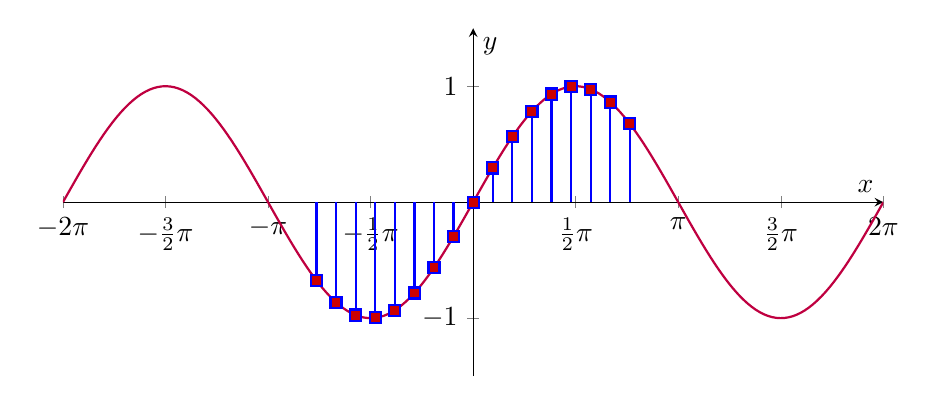
\begin{tikzpicture}
                            \begin{axis}[
                                domain=-2*pi:2*pi,
                                samples=200,
                                axis lines=middle,
                                xlabel=$x$,
                                ylabel=$y$,
                                ymin=-1.5,
                                ymax=1.5,
                                xtick={-2*pi, -3/2*pi, -pi, -1/2*pi, 0, 1/2*pi, pi, 3/2*pi, 2*pi},
                                xticklabels={$-2\pi$, $-\frac{3}{2}\pi$, $-\pi$, $-\frac{1}{2}\pi$, $0$, $\frac{1}{2}\pi$, $\pi$, $\frac{3}{2}\pi$, $2\pi$},
                                ytick={-1, 1},
                                yticklabels={$-1$, $1$},
                                width=12cm,
                                height=6cm
                            ]
                            \addplot [purple, thick] {sin(deg(x))};
                            \addplot+ [blue, thick, ycomb, samples at={-2.4,-2.1,-1.8,-1.5,-1.2,-0.9,-0.6,-0.3,0,0.3,0.6,0.9,1.2,1.5,1.8,2.1,2.4}] {sin(deg(x))};
                            \end{axis}
                        \end{tikzpicture}
                        \caption{\color{purple}{tempo continuo}, \color{blue}{tempo discreto:$T=0.3$}}
                        \label{fig:Dominio del tempo}
                    \end{figure}                        
            }
            \item {Dominio dell'ampiezza (spazio):
                    \begin{itemize}
                        \item{Segnale ad ampiezza continua: $x_{(t)}\ continua$, la grandezza fisica del segnale assume con continuità tutti i valori all'interno di un intervallo}
                        \item {Segnale ad ampiezza discreta: $x_{(t)}\ discreta$,se restringo l'intervallo posso renderla continua, la grandezza fisica puó assumere solo valori discreti}
                    \end{itemize}
                    \begin{figure}[H]
                        \centering
                        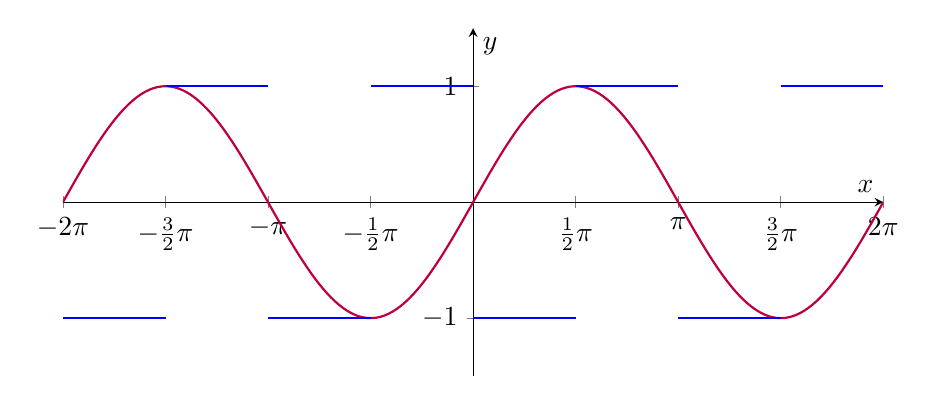
\begin{tikzpicture}
                            \begin{axis}[
                                domain=-2*pi:2*pi,
                                samples=200,
                                axis lines=middle,
                                xlabel=$x$,
                                ylabel=$y$,
                                ymin=-1.5,
                                ymax=1.5,
                                xtick={-2*pi, -3/2*pi, -pi, -1/2*pi, 0, 1/2*pi, pi, 3/2*pi, 2*pi},
                                xticklabels={$-2\pi$, $-\frac{3}{2}\pi$, $-\pi$, $-\frac{1}{2}\pi$, $0$, $\frac{1}{2}\pi$, $\pi$, $\frac{3}{2}\pi$, $2\pi$},
                                ytick={-1, 1},
                                yticklabels={$-1$, $1$},
                                width=12cm,
                                height=6cm
                            ]
                            \addplot [purple, thick] {sin(deg(x))};
                            \addplot [blue, thick, jump mark left] coordinates {
                                (-2*pi,-1) (-3/2*pi,1) (-pi,-1) (-1/2*pi,1) (0,-1) (1/2*pi,1) (pi,-1) (3/2*pi,1) (2*pi,-1)
                            };
                            \end{axis}
                        \end{tikzpicture}
                        \caption{\color{purple}{ampiezza continua}, \color{blue}{ampiezza discreta}}
                        \label{fig:dominio dell'ampiezza}
                    \end{figure}
                    }
        \end{itemize}
        Possiamo costruire una tabella per categorizzare le tipologie di segnali:
        \begin{table}[h]
            \centering
            \begin{tabular}{c|cccc}
            Segnale   & \multicolumn{1}{c|}{Continuo}     & Discreto          & $t$ &  \\ \cline{1-4}
            Continua  & \multicolumn{1}{c|}{Analogico}   & Sequenza/Digitale &       &  \\ \cline{1-3}
            Discreta  & \multicolumn{1}{c|}{Quantizzato} & Binario           &       &  \\
            $x_{(t)}$ &                                  &                   &       & 
            \end{tabular}
        \end{table}

    \section{Segnali Analogici}
    \subsection{Grandezze dei segnali Analogici}
    
        \subsubsection{Potenza istantanea}\label{Potenza istantanea}
                \begin{align}
                    P_{x} & \triangleq |x_{(t)}|^2 \nonumber \\   
                    Se\ x_{(t)} \in &\ \mathbb{R} \rightarrow P_{x} \triangleq x_{(t)}^2 \nonumber
                \end{align}
        \subsubsection{Energia}
            \[
                E_{x} \triangleq \int_{-\infty}^{\infty} P_{x}(t) \,dt = \int_{-\infty}^{\infty} |x_{(t)}|^2 \,dt    
            \]
            \[
                Energia:
                \begin{cases}
                    Energia\ finita \hspace{0.3cm}& (Segali\ fisici) \\
                    Energia\ infinita \hspace{0.3cm}& (Segali\ ideali)
                \end{cases}  
            \]
        \subsubsection{Potenza Media}\label{Potenza media}
            Definiamo il \index{Segnale Troncato}{\bf Segnale Troncato}:
                \[
                    x_{(t)} = X_{(t)} \triangleq 
                    \begin{cases}
                        x_{(t)} \hspace{1cm} -\frac{T}{2} \leq t \leq \frac{T}{2} \\
                        0 \hspace{2cm}altrove
                    \end{cases}
                    \]  
                    \begin{center}
                        \em T = Periodo di osservazione
                    \end{center}
                \begin{figure}[h]
                    \centering
                    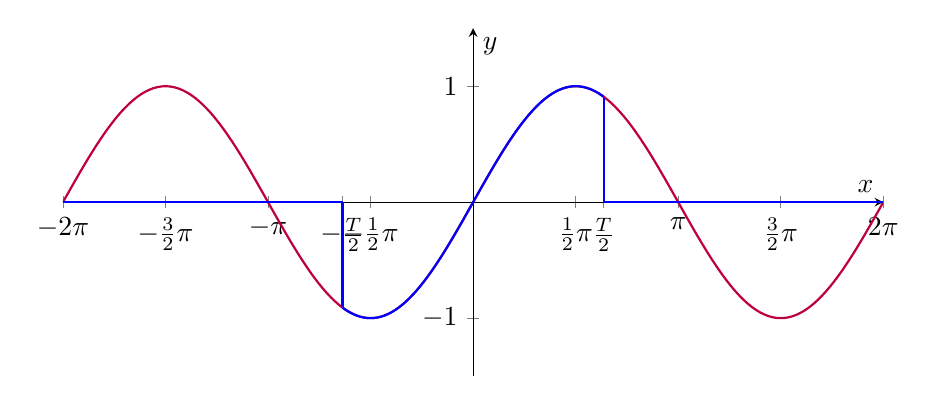
\begin{tikzpicture}
                        \begin{axis}[
                            domain=-2*pi:2*pi,
                            samples=200,
                            axis lines=middle,
                            xlabel=$x$,
                            ylabel=$y$,
                            ymin=-1.5,
                            ymax=1.5,
                            xtick={-2*pi, -3/2*pi, -pi, -1/2*pi,-2, 0, 2,1/2*pi, pi, 3/2*pi, 2*pi},
                            xticklabels={$-2\pi$, $-\frac{3}{2}\pi$, $-\pi$, $-\frac{1}{2}\pi$,$-\frac{T}{2}$, $0$, $\frac{T}{2}$, $\frac{1}{2}\pi$, $\pi$, $\frac{3}{2}\pi$, $2\pi$},
                            ytick={-1, 1},
                            yticklabels={$-1$, $1$},
                            width=12cm,
                            height=6cm
                        ]
                        \addplot [purple, thick] {sin(deg(x))};
                        \addplot [blue, thick, domain = -2:2] {sin(deg(x))};
                        \addplot [blue, thick, domain = 2:2*pi] {0};
                        \addplot [blue, thick, domain = -2*pi:-2] {0};
                        \addplot [const plot, thick,color=blue] coordinates {(-2,-0.9) (-2,0)};
                        \addplot [const plot, thick,color=blue] coordinates {(2,0.9) (2,0)};
                        \end{axis}
                    \end{tikzpicture}
                    \caption{Segnale troncato}
                    \label{fig:troncato}
                \end{figure}
            

            % NON CAPISCO COSA É POTENZA MEDIA E COSA SIA POTENZA ISTANTANEA CHE CAVOLO DI RELAZIONE
            % USO PER PASSARE DA PxT A Px  
            La potenza media é:
            \[
                P_{x_{T}} \triangleq \frac{E_{x_{T}}}{T}    
            \]
            \[
                E_{x_{T}} = \int_{-\frac{T}{2}}^{\frac{T}{2}}  |x_{(t)}|^2 \,dt  
            \]
            dalla quale possiamo ricavare se $T \rightarrow \infty \Rightarrow P_{x_{T}} = P_{x}$:
            \[
                P_{x} \triangleq \lim_{T\rightarrow\infty} \frac{E_{x_{T}}}{T} =\lim_{T\rightarrow\infty} \frac{1}{T} \int_{-\frac{T}{2}}^{\frac{T}{2}}  |x_{(t)}|^2 \,dt    
            \]  
            Possiamo ricavare delle propietá secondo energia e potenza:
            \begin{itemize}
                \item Se $x_{(t)}$ ha $E_x < \infty \Rightarrow P_x = 0$
                \item Se $x_{(t)}$ ha $P_x = k \neq 0 < \infty \Rightarrow E_x = \infty$
            \end{itemize}
        \subsubsection{Valore Efficace}\label{Valore Efficace}
                \[    
                    x_{eff} \triangleq \sqrt{P_{x}}
                \]
        
        \subsubsection{Valore Medio}\label{Valore medio}

                % TO DO: rivedi qui per evitare un page break
                    \[
                        x_{m} \triangleq \lim_{T\rightarrow\infty} \frac{1}{T} \int_{-\infty}^{\infty}  x_{(t)_T} \,dt = \lim_{T\rightarrow\infty} \frac{1}{T} \int_{-\frac{T}{2}}^{\frac{T}{2}}  x_{(t)} \,dt 
                    \]
                    \[
                        x_{(t)_T}\ =\ Segnale\ troncato
                    \]
                    
    \subsection{Analisi energetiche su segnali comuni}
        \subsubsection{Costante}
            $x_{(t)} = A\ \ \forall t$
            \begin{figure}[h]
                \centering
                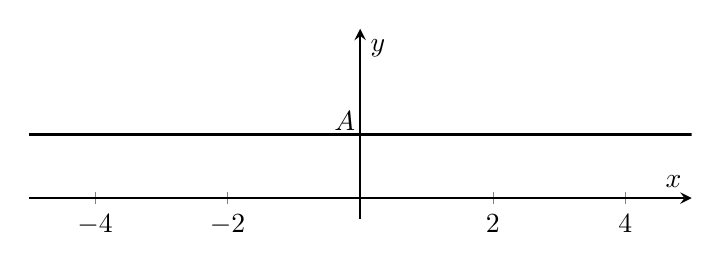
\begin{tikzpicture}
                    \begin{axis}[
                        xlabel=$x$,
                        ylabel=$y$,
                        xmin=-5,
                        xmax=5,
                        ymin=-0.5,
                        ymax=4,
                        ytick = {1.5},
                        yticklabels = {$A$},
                        yticklabel style = {yshift=5pt,xshift=4pt}, 
                        axis lines=middle,
                        thick,
                        domain=-5:5,
                        samples=100,
                        width=10cm,
                        height=4cm
                    ]
                    \addplot [const plot,black, thick] {1.5};
                    \end{axis}
                \end{tikzpicture}
                \caption{Segnale costante}
                \label{fig:segnale costante}
            \end{figure}
            \begin{itemize}
                \item {Energia:
                        \[
                            E_{x} = \int_{-\infty}^{\infty} P_{x}(t) \,dt = \int_{-\infty}^{\infty} |x_{(t)}|^2 \,dt = \int_{-\infty}^{\infty} A^2 \,dt = \infty 
                        \]
                }
                \item {Potenza Media:
                        \[
                            P_{x} = \lim_{T\rightarrow\infty} \frac{E_{x_{T}}}{T} = \lim_{T\rightarrow\infty} \frac{1}{T} \int_{-\frac{T}{2}}^{\frac{T}{2}}  |x_{(t)}|^2 \,dt = \lim_{T\rightarrow\infty} \frac{1}{T} \int_{-\frac{T}{2}}^{\frac{T}{2}} A^2 \,dt = A^2     
                        \]
                }
                \item {Valore Efficace:
                        \[
                            x_{eff} = \sqrt{P_{x}} = \sqrt{A^2} = |A|
                        \]
                }
                \item {Valore Medio:
                        \[
                            x_{m} = \lim_{T\rightarrow\infty} \frac{1}{T} \int_{-\frac{T}{2}}^{\frac{T}{2}}  x_{(t)} \,dt = \lim_{T\rightarrow\infty} \frac{1}{T} \int_{-\frac{T}{2}}^{\frac{T}{2}}  A \,dt = \lim_{T\rightarrow\infty} \frac{1}{T} AT = A 
                        \]
                }
            \end{itemize}
        
        \subsubsection{Cosinusoide}
            $x_{(t)} = A \cos(2 \pi f_0 t +\phi)$\\
            $A = Ampiezza,\  f_0= \frac{1}{T} = frequenza,\ \phi =fase$
            \begin{figure}[H]
                \centering
                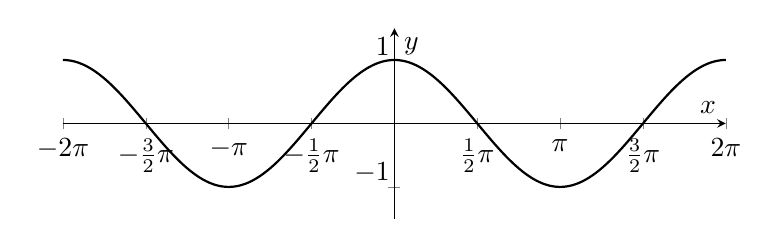
\begin{tikzpicture}
                    \begin{axis}[
                        domain=-2*pi:2*pi,
                        samples=200,
                        axis lines=middle,
                        xlabel=$x$,
                        ylabel=$y$,
                        ymin=-1.5,
                        ymax=1.5,
                        xtick={-2*pi, -3/2*pi, -pi, -1/2*pi, 0,1/2*pi, pi, 3/2*pi, 2*pi},
                        xticklabels={$-2\pi$, $-\frac{3}{2}\pi$, $-\pi$, $-\frac{1}{2}\pi$, $0$, $\frac{1}{2}\pi$, $\pi$, $\frac{3}{2}\pi$, $2\pi$},
                        ytick={-1, 1},
                        yticklabels={$-1$, $1$},
                        yticklabel style = {yshift=5pt,xshift=4pt}, 
                        width=10cm,
                        height=4cm
                    ]
                    \addplot [black, thick] {cos(deg(x))};
                    \end{axis}
                \end{tikzpicture}
                \caption{Segnale cosinusoidale ($\phi = 0$)}
                \label{fig:segnale sinusoidale}
            \end{figure}
            
            \begin{itemize}
                \item {Energia:
                    \[
                        E_{x} = \int_{-\infty}^{\infty} |x_{(t)}|^2 \ dt = \int_{-\infty}^{\infty} A^2 \cos^2(2\pi f_0 t + \phi) dt 
                    \]
                    Ricaviamo dalla $(1)$ \ref{Trigonometria} il $\sin^2(\alpha)$ e lo sostituiamo $(2.1)$ \ref{Trigonometria_Duplicazione} \\ $\cos(2\alpha) = \frac{1+ \cos^2(\alpha)}{2}$
                    \begin{align}
                            &= A^2  \int_{-\infty}^{\infty} \frac{1}{2} + \frac{\cos(4\pi f_0 t + 2\phi)}{2} dt \nonumber \\
                            &= A^2  \int_{-\infty}^{\infty} \frac{1}{2} dt + A^2 \int_{-\infty}^{\infty} \frac{\cos(4\pi f_0 t + 2\phi)}{2} dt \nonumber \\
                            &= \infty +\eval{\frac{A}{2} \frac{1}{4\pi f_0} \sin(4\pi f_0 t) }_{-\infty}^{\infty} = \infty \nonumber
                    \end{align}
                }
                \item {Potenza Media:
                    \begin{align}
                        P_{x} &=\lim_{T\rightarrow\infty}  \frac{1}{T} \int_{-\frac{T}{2}}^{\frac{T}{2}}  |x_{(t)}|^2 \,dt =\lim_{T\rightarrow\infty} \frac{1}{T} \int_{-\frac{T}{2}}^{\frac{T}{2}} A^2 \cos^2(2\pi f_0 t + \phi) dt \nonumber\\
                              &= \lim_{T\rightarrow\infty} \frac{1}{T} \frac{A}{2}T + \lim_{T\rightarrow\infty} \frac{A}{2}\int_{-\frac{T}{2}}^{\frac{T}{2}}\cos(4\pi f_0 t + 2\phi) dt  \nonumber\\
                              &= \frac{A}{2} + \lim_{T\rightarrow\infty} \eval{\frac{A}{2}\frac{1}{4\pi f_0}\sin(4\pi f_0 t + 2\phi)}_{\frac{T}{2}}^{-\frac{T}{2}} = \frac{A^2}{2} \nonumber
                    \end{align}
                }
                \item {Valore Efficace:
                    \[
                        x_{eff} = \sqrt{P_{x}} = \sqrt{\frac{A^2}{2}} =\frac{|A^2|}{\sqrt{2}} 
                    \]
                }
                \item {Valore Medio:
                    \begin{align}
                        x_{m} &= \lim_{T\rightarrow\infty} \frac{1}{T} \int_{-\frac{T}{2}}^{\frac{T}{2}}  x_{(t)} \,dt =\lim_{T\rightarrow\infty} \frac{1}{T} \int_{-\frac{T}{2}}^{\frac{T}{2}}\cos(2\pi f_0 t+\phi) dt \nonumber \\
                              &= \lim_{T\rightarrow\infty} \frac{1}{T}  \eval{\frac{A}{2}\frac{1}{2\pi f_0}\sin(2\pi f_0 t + \phi)}_{\frac{T}{2}}^{-\frac{T}{2}} = 0 \nonumber
                    \end{align}
                }
            \end{itemize}

            %Richimo per il label del formulario $(1)$ e $(2)$ \ref{Trigonometria} 
        \pagebreak
        \subsubsection{Gradino}
        $U_{(t)} = x_{(t)} = 
            \begin{cases}
                1 & t > 0 \\
                0 & t \leq 0  
            \end{cases}
        $
        \begin{figure}[H]
            \centering
            \begin{tikzpicture}
                \begin{axis}[
                    xlabel=$x$,
                    ylabel=$y$,
                    xmin=-5,
                    xmax=5,
                    ymin=-0.5,
                    ymax=4,
                    ytick = {1.5},
                    xtick = {},
                    xticklabels = {},
                    yticklabels = {$A$},
                    yticklabel style = {yshift=5pt,xshift=4pt}, 
                    axis lines=middle,
                    thick,
                    domain=-5:5,
                    samples=100,
                    width=10cm,
                    height=4cm
                ]
                \addplot [const plot,red, thick] coordinates{(0,1.5)(5,1.5)};
                \addplot [const plot,red, thick] coordinates{(0,0)(0,1.5)};
                \addplot [const plot,red, thick] coordinates{(-5,0)(0,0)};
                \end{axis}
            \end{tikzpicture}
            \caption{Segnale gradino}
            \label{fig:segnale gradino}
            
        \end{figure}        

        \begin{itemize}
            \item {Energia:
                \[
                    E_{x} = \int_{-\infty}^{\infty} |x_{(t)}|^2 \ dt = \int_{0}^{\infty} 1\ dt = \infty 
                \]
            }
            \item {Potenza Media:
                \[
                    P_{x} =\lim_{T\rightarrow\infty}  \frac{1}{T} \int_{-\frac{T}{2}}^{\frac{T}{2}}  |U_{(t)}|^2 \,dt =\lim_{T\rightarrow\infty} \frac{1}{T} \int_{0}^{\frac{T}{2}} 1\ dt = \lim_{T\rightarrow\infty} \frac{1}{T} \frac{T}{2} = \frac{1}{2}
                \]
            }
            \item {Valore Efficace:
                \[
                    x_{eff} = \sqrt{P_{x}} = \frac{1}{\sqrt{2}} 
                \]
            }
            \item {Valore Medio:
                    \[x_{m} = \lim_{T\rightarrow\infty} \frac{1}{T} \int_{-\frac{T}{2}}^{\frac{T}{2}}  x_{(t)} \,dt =\lim_{T\rightarrow\infty} \frac{1}{T} \int_{0}^{\frac{T}{2}} 1\ dt = \lim_{T\rightarrow\infty} \frac{1}{T} \frac{T}{2} = \frac{1}{2} \]
            }
        \end{itemize}
        
        \subsubsection{Rettangolo}
        $x_{(t)} = A\hspace{0.1cm}rect\left(\frac{t}{T}\right) =
            \begin{cases}
                A & -\frac{t}{T}\leq t\leq \frac{t}{T}\\
                0 & Altrove 
            \end{cases}
        $
        \begin{figure}[H]
            \centering
            \begin{tikzpicture}
                \begin{axis}[
                    xlabel=$x$,
                    ylabel=$y$,
                    xmin=-5,
                    xmax=5,
                    ymin=-0.5,
                    ymax=4,
                    ytick = {1.5},
                    xtick={-1.5, 0, 1.5},
                    xticklabels={$-\frac{T}{2}$, $0$, $\frac{T}{2}$},
                    yticklabels = {$A$},
                    yticklabel style = {yshift=5pt,xshift=4pt}, 
                    axis lines=middle,
                    thick,
                    domain=-5:5,
                    samples=100,
                    width=10cm,
                    height=4cm
                ]
                \addplot [const plot,red, thick] coordinates{(-1.5,1.5)(1.5,1.5)};
                \addplot [const plot,red, thick] coordinates{(-1.5,0)(-1.5,1.5)};
                \addplot [const plot,red, thick] coordinates{(1.5,0)(1.5,1.5)};
                \addplot [const plot,red, thick] coordinates{(5,0)(1.5,0)};
                \addplot [const plot,red, thick] coordinates{(-5,0)(-1.5,0)};
                \end{axis}
              \end{tikzpicture}
            \caption{Segnale rettangolo}
            \label{fig:segnale rettangolo}
        \end{figure}        
        \begin{itemize}
            \item {Energia:
                \[
                    E_{x} = \int_{-\infty}^{\infty} |x_{(t)}|^2 \ dt = \int_{-\frac{T}{2}}^{\frac{T}{2}} A^2 \hspace{0.1cm}rect^2\left(\frac{t}{T}\right)\ dt = A^2 \int_{-\frac{T}{2}}^{\frac{T}{2}}  1\ dt = A^2 T 
                \]
            }
            \item {Potenza Media:
                $T < T_0$ se non fosse cosí avrei una costante
                \begin{align}
                    P_{x} =\lim_{T\rightarrow\infty}  \frac{1}{T_0} \int_{-\frac{T_0}{2}}^{\frac{T_0}{2}}  |x_{(t)}|^2 \,dt & =\lim_{T\rightarrow\infty} \frac{1}{T_0}\int_{-\frac{T_0}{2}}^{\frac{T_0}{2}} A^2 \hspace{0.1cm}rect^2\left(\frac{t}{T}\right)\ dt \nonumber \\
                         & =\lim_{T\rightarrow\infty} \frac{1}{T_0} A^2 T = 0 \nonumber
                \end{align}
            }
            \item {Valore Efficace:
                \[
                    x_{eff} = \sqrt{P_{x}} = 0 
                \]
            }
            \item {Valore Medio:
                    \begin{align}
                        x_{m} = \lim_{T\rightarrow\infty} \frac{1}{T} \int_{-\frac{T}{2}}^{\frac{T}{2}}  x_{(t)} \,dt & = \lim_{T\rightarrow\infty} \frac{1}{T_0}\int_{-\frac{T_0}{2}}^{\frac{T_0}{2}} A\hspace{0.1cm}rect\left(\frac{t}{T}\right)\ dt \nonumber \\
                        & =\lim_{T\rightarrow\infty} \frac{1}{T_0} A T = 0 \nonumber
                    \end{align}
                    \begin{figure}[H]
                        \centering
                        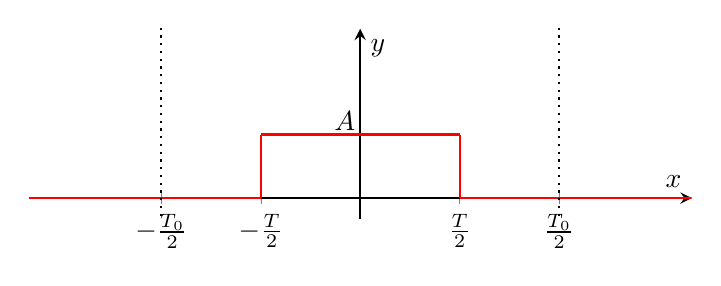
\begin{tikzpicture}
                            \begin{axis}[
                                xlabel=$x$,
                                ylabel=$y$,
                                xmin=-5,
                                xmax=5,
                                ymin=-0.5,
                                ymax=4,
                                ytick = {1.5},
                                xtick={-3,-1.5, 0, 1.5,3},
                                xticklabels={$-\frac{T_0}{2}$,$-\frac{T}{2}$, $0$, $\frac{T}{2}$, $\frac{T_0}{2}$},
                                yticklabels = {$A$},
                                yticklabel style = {yshift=5pt,xshift=4pt}, 
                                axis lines=middle,
                                thick,
                                domain=-5:5,
                                samples=100,
                                width=10cm,
                                height=4cm
                            ]
                            \addplot [const plot,red, thick] coordinates{(-1.5,1.5)(1.5,1.5)};
                            \addplot [const plot,red, thick] coordinates{(-1.5,0)(-1.5,1.5)};
                            \addplot [const plot,red, thick] coordinates{(1.5,0)(1.5,1.5)};
                            \addplot [const plot,red, thick] coordinates{(5,0)(1.5,0)};
                            \addplot [const plot,red, thick] coordinates{(-5,0)(-1.5,0)};
                            \addplot [const plot,dotted, black, thick] coordinates{(3,-5)(3,5)};
                            \addplot [const plot,dotted, black, thick] coordinates{(-3,-5)(-3,5)};
                            \end{axis}
                          \end{tikzpicture}
                        \caption{}
                        \label{fig:segnale rettangolo valore medio}
                    \end{figure}
            }
        \end{itemize}
        
        
        \subsubsection{Esponenziale unilatera}
        $x_{(t)} = e^{-t}U_{(t)}$
        \begin{figure}[H]
            \centering
            \begin{tikzpicture}
                \begin{axis}[
                    xlabel=$x$,
                    ylabel=$y$,
                    xmin=-5,
                    xmax=5,
                    ymin=-0.5,
                    ymax=4,
                    ytick = {1},
                    xtick={},
                    xticklabels={},
                    yticklabels = {$1$},
                    axis lines=middle,
                    thick,
                    domain=-5:5,
                    samples=100,
                    width=10cm,
                    height=4cm
                ]
                \addplot [domain= 0:5,samples = 100,red, thick] {exp(-x)};
                \end{axis}
              \end{tikzpicture}
            \caption{Segnale esponenziale unilatera}
            \label{fig:segnale esponenziale unilatera}
        \end{figure}        
        \begin{itemize}
            \item {Energia:
                \[
                    E_{x} = \int_{-\infty}^{\infty} |x_{(t)}|^2 \ dt = \int_{0}^{\infty} e^{-2t}\ dt = \eval*{-\frac{1}{2} e^{-2t}}_{0}^{\infty} = \frac{1}{2} 
                \]
            }
            \item {Potenza Media:
                \begin{align}
                    P_{x} & =\lim_{T\rightarrow\infty}  \frac{1}{T} \int_{-\frac{T}{2}}^{\frac{T}{2}}  |e^{-t}U_{(t)}|^2 \,dt =\lim_{T\rightarrow\infty} \frac{1}{T} \int_{0}^{\frac{T}{2}} e^{-2t}\ dt \nonumber \\
                          & = \lim_{T\rightarrow\infty} \frac{1}{T} \eval*{\left(-\frac{1}{2}\right) e^{-2t}}_{0}^{\frac{T}{2}} =\lim_{T\rightarrow\infty}-\frac{1}{2T} e^{-2\frac{T}{2}} + \lim_{T\rightarrow\infty} \frac{1}{2T} = 0 \nonumber 
                \end{align}
            }
            \item {Valore Efficace:
                \[
                    x_{eff} = \sqrt{P_{x}} = 0 
                \]
            }
            \item {Valore Medio:
                    \begin{align}
                        x_{m} & = \lim_{T\rightarrow\infty} \frac{1}{T} \int_{-\frac{T}{2}}^{\frac{T}{2}}  x_{(t)} \,dt =\lim_{T\rightarrow\infty} \frac{1}{T} \int_{-\frac{T}{2}}^{\frac{T}{2}} e^{-t}U_{(t)}\,dt = \lim_{T\rightarrow\infty} \frac{1}{T} \int_{0}^{\frac{T}{2}} e^{-t}\,dt \nonumber \\
                              & = \lim_{T\rightarrow\infty} \frac{1}{T} \eval*{(-1) e^{-t}}_{0}^{\frac{T}{2}} =  \lim_{T\rightarrow\infty}-\frac{1}{T} e^{-\frac{T}{2}} + \lim_{T\rightarrow\infty} \frac{1}{T} = 0 \nonumber
                    \end{align}
            }
        \end{itemize}
        
        \pagebreak
        \subsubsection{Esponenziale bilatera}
        $x_{(t)} = e^{-|t|}$
        \begin{figure}[H]
            \centering
            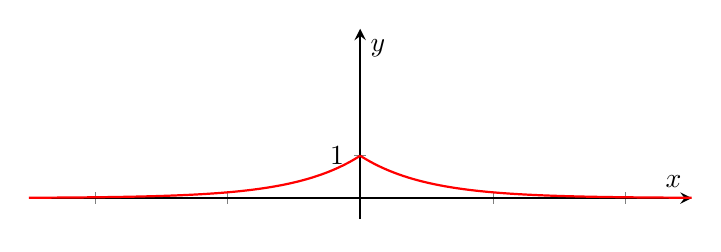
\begin{tikzpicture}
                \begin{axis}[
                    xlabel=$x$,
                    ylabel=$y$,
                    xmin=-5,
                    xmax=5,
                    ymin=-0.5,
                    ymax=4,
                    ytick = {1},
                    xtick={},
                    xticklabels={},
                    yticklabels = {$1$},
                    axis lines=middle,
                    thick,
                    domain=-5:5,
                    samples=100,
                    width=10cm,
                    height=4cm
                ]
                \addplot [domain= 0:5,samples = 100,red, thick] {exp(-x)};
                \addplot [domain= -5:0,samples = 100,red, thick] {exp(x)};
                \end{axis}
              \end{tikzpicture}
            \caption{Segnale esponenziale bilatera}
            \label{fig:segnale esponenziale bilatera}
        \end{figure}        
        \begin{itemize}
            \item {Energia:
                \[
                    E_{x} = \int_{-\infty}^{\infty} |x_{(t)}|^2 \ dt =2 \int_{0}^{\infty} e^{-2t}\ dt = \eval*{2 \left(-\frac{1}{2}\right) e^{-2t}}_{0}^{\infty} = 1 
                \]
            }
            \item {Potenza Media:
                \begin{align}
                    P_{x} & =\lim_{T\rightarrow\infty}  \frac{1}{T} \int_{-\frac{T}{2}}^{\frac{T}{2}}  |e^{-t}U_{(t)}|^2 \,dt =\lim_{T\rightarrow\infty} \frac{2}{T} \int_{0}^{\frac{T}{2}} e^{-2t}\ dt \nonumber \\
                          & = \lim_{T\rightarrow\infty} \frac{1}{T} \eval*{e^{-2t}}_{0}^{\frac{T}{2}} =\lim_{T\rightarrow\infty}-\frac{1}{T} e^{-2\frac{T}{2}} + \lim_{T\rightarrow\infty} \frac{1}{T} = 0 \nonumber 
                \end{align}
            }
            \item {Valore Efficace:
                \[
                    x_{eff} = \sqrt{P_{x}} = 0 
                \]
            }
            \item {Valore Medio:
                    \begin{align}
                        x_{m} & = \lim_{T\rightarrow\infty} \frac{1}{T} \int_{-\frac{T}{2}}^{\frac{T}{2}}  x_{(t)} \,dt =\lim_{T\rightarrow\infty} \frac{1}{T} \int_{-\frac{T}{2}}^{\frac{T}{2}} e^{-t}U_{(t)}\,dt = \lim_{T\rightarrow\infty} \frac{1}{T} 2\int_{0}^{\frac{T}{2}} e^{-t}\,dt \nonumber \\
                              & = \lim_{T\rightarrow\infty} \frac{1}{T} \eval*{(-2) e^{-t}}_{0}^{\frac{T}{2}} =  \lim_{T\rightarrow\infty}-\frac{2}{T} e^{-\frac{T}{2}} + \lim_{T\rightarrow\infty} \frac{2}{T} = 0 \nonumber
                    \end{align}
            }
        \end{itemize}        

        \subsubsection{segno $sgn(x_{(t)})$}
        $x_{(t)} = sgn(t) =
            \begin{cases}
                -1 & t < 0\\
                1  & t>0 
            \end{cases}
        $
        \begin{figure}[H]
            \centering
            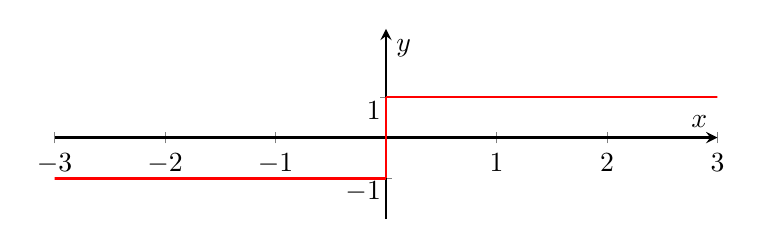
\begin{tikzpicture}
                \begin{axis}[
                    xlabel=$x$,
                    ylabel=$y$,
                    xmin=-3,
                    xmax=3,
                    ymin=-3,
                    ymax=4,
                    ytick={-1.5, 0, 1.5},
                    yticklabels = {$-1$,$0$,$1$},
                    yticklabel style = {yshift=-5pt,xshift=4pt}, 
                    axis lines=middle,
                    thick,
                    domain=-5:5,
                    samples=100,
                    width=10cm,
                    height=4cm
                ]
                \addplot [const plot,red, thick] coordinates{(0,1.5)(5,1.5)};
                \addplot [const plot,red, thick] coordinates{(0,-1.5)(0,1.5)};
                \addplot [const plot,red, thick] coordinates{(0,-1.5)(-5,-1.5)};
                \end{axis}
              \end{tikzpicture}
            \caption{Segnale sgn(x)}
            \label{fig:segnale sgn(x)}
        \end{figure}
        \begin{itemize}
            \item {Energia:
                \[
                    E_{x} = \int_{-\infty}^{\infty} |x_{(t)}|^2 \ dt = \int_{-\infty}^{\infty} sgn^2(t)\ dt = \int_{-\infty}^{\infty} 1\ dt =\infty 
                \]
            }
            \item {Potenza Media:
                \[
                    P_{x} =\lim_{T\rightarrow\infty}  \frac{1}{T} \int_{-\frac{T}{2}}^{\frac{T}{2}}  |x_{(t)}|^2 \,dt =\lim_{T\rightarrow\infty} \frac{1}{T} \int_{-\frac{T}{2}}^{\frac{T}{2}} sgn^2{t}\ dt = \lim_{T\rightarrow\infty} \frac{1}{T} T = 1
                \]
            }
            \item {Valore Efficace:
                \[
                    x_{eff} = \sqrt{P_{x}} = 1 
                \]
            }
            \item {Valore Medio:
                \begin{align}
                    x_{m} & = \lim_{T\rightarrow\infty} \frac{1}{T} \int_{-\frac{T}{2}}^{\frac{T}{2}}  x_{(t)} \,dt =\lim_{T\rightarrow\infty} \frac{1}{T} \int_{-\frac{T}{2}}^{\frac{T}{2}} sgn(t)\ dt \nonumber \\
                          & = \lim_{T\rightarrow\infty} \frac{1}{T} \left[\int_{-\frac{T}{2}}^{0}  1\,dt + \int_{0}^{\frac{T}{2}}  1\,dt\right] = \lim_{T\rightarrow\infty} \frac{1}{T} \left(-\frac{T}{2}+\frac{T}{2}\right) = 0 \nonumber
                \end{align}        
            }
        \end{itemize}
        
        \subsection{Segnal Periodici}
            Un segnale é periodico se: \\ 
            \[x_{(t)}=x_{(t-kT_0)}\hspace{0.5cm} k\in\mathbb{Z},\ t_0\in\mathbb{R}^+,\ T_0 = Periodo\ del\ segnale\]
            \begin{figure}[H]
                \centering
                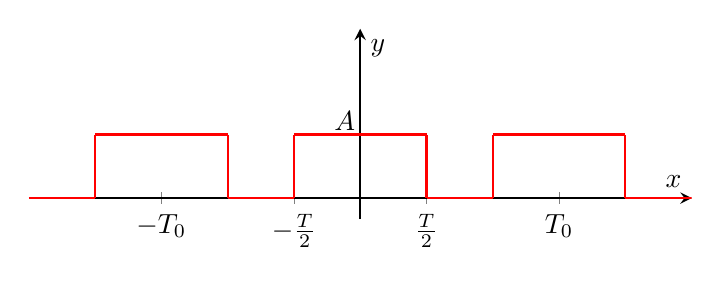
\begin{tikzpicture}
                    \begin{axis}[
                        xlabel=$x$,
                        ylabel=$y$,
                        xmin=-5,
                        xmax=5,
                        ymin=-0.5,
                        ymax=4,
                        ytick = {1.5},
                        xtick={-3,-1, 0, 1,3},
                        xticklabels={$-T_0$,$-\frac{T}{2}$, $0$, $\frac{T}{2}$,$T_0$},
                        yticklabels = {$A$},
                        yticklabel style = {yshift=5pt,xshift=4pt}, 
                        axis lines=middle,
                        thick,
                        domain=-5:5,
                        samples=100,
                        width=10cm,
                        height=4cm
                    ]
                    \addplot [const plot,red, thick] coordinates{(-1,1.5)(1,1.5)};
                    \addplot [const plot,red, thick] coordinates{(-1,0)(-1,1.5)};
                    \addplot [const plot,red, thick] coordinates{(1,0)(1,1.5)};
                    
                    \addplot [const plot,red, thick] coordinates{(-2,1.5)(-4,1.5)};
                    \addplot [const plot,red, thick] coordinates{(-2,0)(-2,1.5)};
                    \addplot [const plot,red, thick] coordinates{(-4,0)(-4,1.5)};
                    
                    \addplot [const plot,red, thick] coordinates{(2,1.5)(4,1.5)};
                    \addplot [const plot,red, thick] coordinates{(2,0)(2,1.5)};
                    \addplot [const plot,red, thick] coordinates{(4,0)(4,1.5)};
                    
                    \addplot [const plot,red, thick] coordinates{(2,0)(1,0)};
                    \addplot [const plot,red, thick] coordinates{(-2,0)(-1,0)};
                    \addplot [const plot,red, thick] coordinates{(-4,0)(-5,0)};
                    \addplot [const plot,red, thick] coordinates{(4,0)(5,0)};
                
                    \end{axis}
                  \end{tikzpicture}
                \caption{Segnale periodico}
                \label{fig:segnale periodico}
            \end{figure}     
            Si definiscono le seguenti grandezze: 
            \begin{itemize}
                \item {Energia di un segnale periodico
                    \begin{align}
                        E_{x} & = \int_{-\infty}^{\infty}  |x_{(t)}|^2 \,dt =\sum_{k=-\infty}^{\infty}\int_{-\frac{T_0}{2}+kT_0}^{\frac{T_0}{2}+kT_0} |x_{(t)}|^2 dt =\sum_{k=-\infty}^{\infty} X  \nonumber \\
                            & = \lim_{k\rightarrow\infty} kX= \infty \nonumber
                    \end{align}
                    Tutti i segnali periodici hanno quindi $E_x = \infty$   
                }
                \item {Potenza media di un segnale periodico
                    \begin{align}
                        P_{x} & = \lim_{T\rightarrow\infty} \frac{1}{T} \int_{-\frac{T}{2}}^{\frac{T}{2}}  |x_{(t)}|^2 \,dt\Rightarrow T = kT_0 \Rightarrow \lim_{k\rightarrow\infty} \frac{1}{kT_0} \int_{-\frac{kT_0}{2}}^{\frac{kT_0}{2}} |x_{(t)}|^2 dt \nonumber \\
                            & = \lim_{k\rightarrow\infty} \frac{1}{kT_0} k \int_{-\frac{T_0}{2}}^{\frac{T_0}{2}} |x_{(t)}|^2 dt  = \frac{1}{T_0} \int_{-\frac{T_0}{2}}^{\frac{T_0}{2}} |x_{(t)}|^2 dt \nonumber
                    \end{align}      
                    Posso calcolare la potenza di un singolo periodo:
                    \[
                        P_x = \frac{1}{T_0} \int_{-\frac{T_0}{2}}^{\frac{T_0}{2}} |x_{(t)}|^2 dt  
                    \]
                }
                \item {Valore medio di un segnale periodico
                    \[
                        x_m = \frac{1}{T_0} \int_{-\frac{T_0}{2}}^{\frac{T_0}{2}} x_{(t)} dt  
                    \]
                }
            \end{itemize}   
    \section{Trasformata Serie Di Fourier}
    \subsection{Segnale Periodico}
        Si definisce segnale periodico un segnale tale che:
        \[
            x_{(t)} = x_{(t-kT_0)}    
        \]
        \[
            T_0=Periodo\ \ \ f_0\triangleq \frac{1}{T_0} =Frequenza
        \]
    \subsection{Trasformata Serie Di Fourier}
        Ogni segnale periodico di periodo $T_0$ che soddifa le condizioni di Dirichlet e la sua $E_x < \infty (C.S.)$ puó essere scritto come la somma di 
        infinite sinusoidi di frequenze multiple di $f_0 = \frac{1}{T_0}$
        \begin{itemize}
            \item{Equazione di Sintesi - Antitrasformata(ATSF)\label{ATSF}
                \[
                    x_{(t)} = \sum_{k = -\infty}^{\infty} X_{k} e^{j2\pi kf_0t} \hspace{1cm} X_{k}\in \mathbb{C},\ f_0 = \frac{1}{T_0} 
                \]
                Se lo sviluppassimo sarebbe composto da:
                \[
                   x_{(t)} =\ldots  + X_{-1} e^{j2\pi (-1)f_0t} + X_{0} + X_{1} e^{j2\pi (1) f_0t} + \ldots 
                \]
                $X_0$ corrisponde al Valore medio \ref{Valore medio} del segnale, inoltre le componenti $X_k$ prendono il nome di armoniche alla frequenza $f$ corrispondente
            }
            \item{Equazione di Analisi - Trasformata(TSF)\label{TSF}
                \[
                    X_k =\frac{1}{T_0}\int_{-\frac{T_0}{2}}^{\frac{T_0}{2}} x_{(t)} e^{-j2\pi kf_0t} dt
                \]
            } 
        \end{itemize}
        La TSF gode della biunivocitá: $\forall x_{(t)} \exists! X_k$:
        \begin{align}
            x_{(t)} & \overunderset{TSF}{ATSF}{\rightleftharpoons} X_k  \nonumber\\
            Segnale\ Analogico\ Periodico &\overunderset{TSF}{ATSF}{\rightleftharpoons} Sequenza\ Complessa \nonumber
        \end{align}
        \subsubsection{Rappresentazione di $X_k$}
            Essendo $X_k$ un numero complesso puó essere rappresentato in forma polare: 
            \[
                X_k = |X_k|e^{\angle X_k}  
            \]
            Si possono rappresentare il modulo (Ampiezza) e la fase tramite grafici che prendono il nome di spettri:
            \begin{figure}[H]
                \centering
                \subfloat[Spettro di Ampiezza]{
                    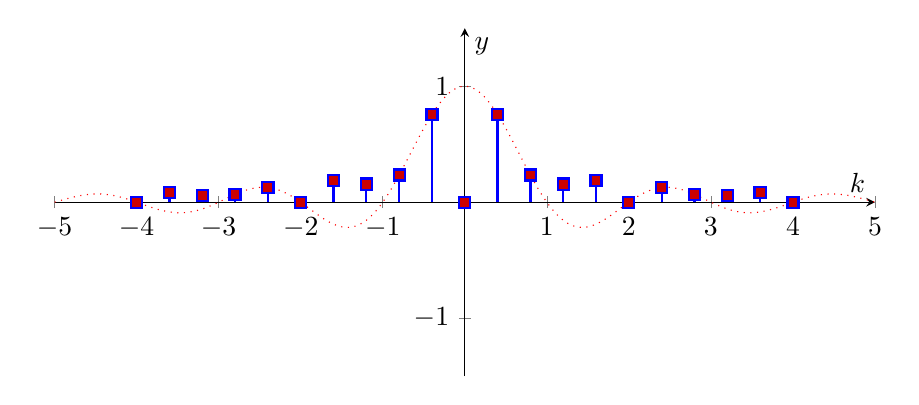
\begin{tikzpicture}
                        \begin{axis}[
                            domain=-5:5,
                            samples=200,
                            axis lines=middle,
                            xlabel=$k$,
                            ylabel=$y$,
                            ymin=-1.5,
                            ymax=1.5,
                            xtick={-5,-4,-3,-2,-1,0,1,2,3,4,5},
                            xticklabels={$-5$,$-4$,$-3$,$-2$,$-1$,$0$,$1$,$2$,$3$,$4$,$5$},
                            ytick={-1, 1},
                            yticklabels={$-1$, $1$},
                            width=12cm,
                            height=6cm
                        ]
                        \addplot [red,dotted, samples = 300] {sin(deg(x*pi))/(x*pi)};
                        \addplot+ [blue, thick, ycomb, samples at={-4,-3.6,-3.2,-2.8,-2.4,-2,-1.6,-1.2,-0.8,-0.4,0,0.4,0.8,1.2,1.6,2,2.4,2.8,3.2,3.6,4}] {abs(sin(deg(x*pi))/(x*pi))};
                        \end{axis}
                    \end{tikzpicture}
                }
                \hfill
                \subfloat[Spettro di Fase]{
                    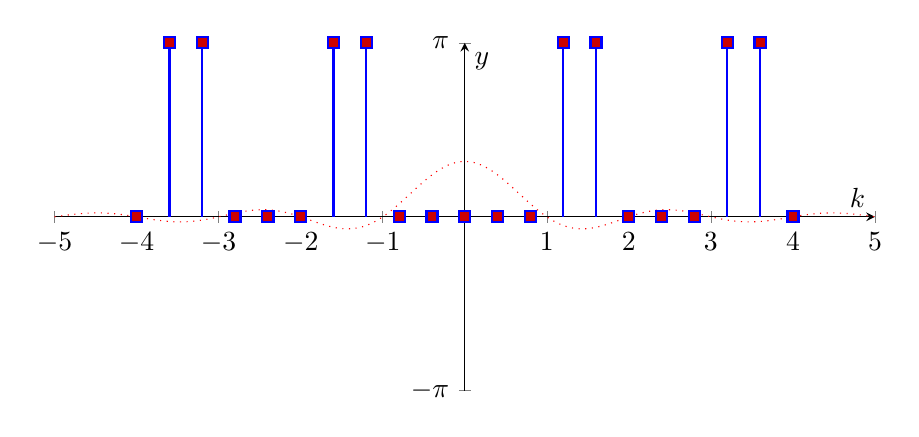
\begin{tikzpicture}
                        \begin{axis}[
                            domain=-5:5,
                            samples=200,
                            axis lines=middle,
                            xlabel=$k$,
                            ylabel=$y$,
                            ymin=-pi,
                            ymax=pi,
                            xtick={-5,-4,-3,-2,-1,0,1,2,3,4,5},
                            xticklabels={$-5$,$-4$,$-3$,$-2$,$-1$,$0$,$1$,$2$,$3$,$4$,$5$},
                            ytick={-pi, pi},
                            yticklabels={$-\pi$, $\pi$},
                            width=12cm,
                            height=6cm
                        ]
                        \addplot [red,dotted, samples = 300] {sin(deg(x*pi))/(x*pi)};
                        \addplot+ [blue, thick, ycomb, samples at={-4,-3.6,-3.2,-2.8,-2.4,-2,-1.6,-1.2,-0.8,-0.4,0,0.4,0.8,1.2,1.6,2,2.4,2.8,3.2,3.6,4}] {rad(atan2(0,sin(deg(x*pi))/(x*pi)))};
                        \end{axis}
                    \end{tikzpicture}
                }
                \caption{Spettro di un treno di rect}
            \end{figure}
            lo spettro di Ampiezza gode della \textbf{simmetria pari} rispetto alle ascisse quindi é \textbf{sempre positivo}, mentre lo spettro di fase della \textbf{simmetria dispari}.
        \subsection{Propietá della TSF}
            \subsection{Linearitá}
            \subsection{Simmetria Hermitiana}
        
        \subsection{Calcolo dei coefficienti $X_k$ per segnali noti}
            \subsubsection{$A\cos(2\pi f_0 t)$}
                $x_{(t)}=A\cos(2\pi f_0 t), \hspace{0.3cm} A>0$
                \begin{align}
                    ATSF[x_{(t)}] & = ATSF[A\cos(2\pi f_0 t)] \nonumber \\
                        & = ATSF[\frac{A}{2} (e^{j2\pi kf_0t} + e^{-j2\pi kf_0t})] \nonumber 
                \end{align}
                Utilizzando la composizione dei coefficienti $X_k$:
                \begin{align}
                    x_{(t)} & =\ldots  + X_{-1} e^{j2\pi (-1)f_0t} + X_{0} + X_{1} e^{-j2\pi (1) f_0t} + \ldots \nonumber\\
                    Abbiamo:& \nonumber 
                \end{align}
                        \[X_{-1} = \frac{A}{2}\hspace{.3cm} X_{0} = 0\hspace{.3cm} X_{1} = \frac{A}{2}\] 
                Possiamo tracciare lo spettro del segnale:
                \begin{figure}[H]
                    \centering
                    \subfloat[Spettro di Ampiezza]{
                    \begin{tikzpicture}
                        \begin{axis}[
                            domain=-4:4,
                            samples=200,
                            axis lines=middle,
                            xlabel=$t$,
                            ylabel=$y$,
                            ymin=-1.5,
                            ymax=1.5,
                            xtick={-5,-4,-3,-2,-1,0,1,2,3,4,5},
                            xticklabels={$-5$,$-4$,$-3$,$-2$,$-1$,$0$,$1$,$2$,$3$,$4$,$5$},
                            ytick={1},
                            yticklabels={$\frac{A}{2}$},
                            width=6.5cm,
                            height=5cm
                            ]
                            \addplot [const plot,black,dotted] coordinates{(-4,1)(4,1)};
                            \addplot+ [blue, thick, ycomb, samples at = {-1,1}] {1};
                            \end{axis}
                        \end{tikzpicture}
                    }
                    \hfill
                    \subfloat[Spettro di Fase]{
                        \begin{tikzpicture}
                            \begin{axis}[
                                domain=-4:4,
                                samples=200,
                                axis lines=middle,
                                xlabel=$t$,
                                ylabel=$y$,
                                ymin=-pi,
                                ymax=pi,
                                xtick={-5,-4,-3,-2,-1,0,1,2,3,4,5},
                                xticklabels={$-5$,$-4$,$-3$,$-2$,$-1$,$0$,$1$,$2$,$3$,$4$,$5$},
                                ytick={-pi, pi},
                                yticklabels={$-\pi$, $\pi$},
                                width=6.5cm,
                                height=5cm
                            ]
                            \addplot+ [blue, thick, ycomb, samples at = {-4,-3,-2,-1,0,1,2,3,4}] {0};
                            \end{axis}
                        \end{tikzpicture}
                    }
                    \caption{Spettro TSF del coseno $A>0$}
                \end{figure}
            \subsubsection{$A\sin(2\pi f_0 t)$}
                $x_{(t)}=A\sin(2\pi f_0 t), \hspace{0.3cm} A>0$
                \begin{align}
                    ATSF[x_{(t)}] & = ATSF[A\sin(2\pi f_0 t)] \nonumber \\
                        & = ATSF[\frac{A}{2} (e^{j2\pi kf_0t} - e^{-j2\pi kf_0t})] \nonumber 
                \end{align}
                Utilizzando la composizione dei coefficienti $X_k$:
                \begin{align}
                    x_{(t)} & =\ldots  + X_{-1} e^{j2\pi (-1)f_0t} - X_{0} + X_{1} e^{-j2\pi (1) f_0t} + \ldots \nonumber\\
                    Abbiamo:& \nonumber 
                \end{align}
                        \[X_{-1} = -\frac{A}{2j}\hspace{.3cm} X_{0} = 0\hspace{.3cm} X_{1} = \frac{A}{2j}\] 
                \[
                    |X_k|= 
                    \begin{cases}
                            |\frac{A}{2j}| = \frac{A}{2} \hspace{0.5cm} & k= 1\\
                            |-\frac{A}{2j}| = \frac{A}{2} \hspace{0.5cm} & k= -1\\
                            0 \hspace{0.5cm} & altrove  \\
                    \end{cases}
                    \hspace{0.5cm}
                    \angle X_k= 
                    \begin{cases}
                        \angle \frac{A}{2j} = -\frac{\pi}{2} \hspace{0.5cm} & k= 1\\
                        \angle |-\frac{A}{2j}| = \frac{\pi}{2} \hspace{0.5cm} & k= -1\\
                        0 \hspace{0.5cm} & altrove  \\
                    \end{cases}
                    \]
                Possiamo tracciare lo spettro del segnale:
                \begin{figure}[H]
                    \centering
                    \subfloat[Spettro di Ampiezza]{
                        \begin{tikzpicture}
                            \begin{axis}[
                                domain=-4:4,
                                samples=200,
                                axis lines=middle,
                                xlabel=$t$,
                                ylabel=$y$,
                                ymin=-1.5,
                                ymax=1.5,
                                xtick={-5,-4,-3,-2,-1,0,1,2,3,4,5},
                                xticklabels={$-5$,$-4$,$-3$,$-2$,$-1$,$0$,$1$,$2$,$3$,$4$,$5$},
                                ytick={1},
                                yticklabels={$\frac{A}{2}$},
                                width=6.5cm,
                                height=5cm
                                ]
                                \addplot [const plot,black,dotted] coordinates{(-4,1)(4,1)};
                                \addplot+ [blue, thick,mark = triangle*, ycomb, samples at = {-1,1}] {1};
                                \end{axis}
                            \end{tikzpicture}
                        }
                    \hfill
                    \subfloat[Spettro di Fase]{
                            \begin{tikzpicture}
                                \begin{axis}[
                                    domain=-4:4,
                                    samples=200,
                                    axis lines=middle,
                                    xlabel=$t$,
                                    ylabel=$y$,
                                    ymin=-pi,
                                    ymax=pi,
                                    xtick={-5,-4,-3,-2,-1,0,1,2,3,4,5},
                                    xticklabels={$-5$,$-4$,$-3$,$-2$,$-1$,$0$,$1$,$2$,$3$,$4$,$5$},
                                    ytick={-pi,-1/2*pi,1/2*pi, pi},
                                    yticklabels={$-\pi$,$-\frac{\pi}{2}$,$\frac{\pi}{2}$ $\pi$},
                                    yticklabel style = {xshift=3pt}, 
                                    width=6.5cm,
                                    height=5cm
                                ]
                                \addplot+ [blue, thick,mark = square*,const plot] coordinates{(-1,1/2*pi)(-1,0)};
                                \addplot+ [blue, thick,mark = square*,const plot] coordinates{(1,-1/2*pi)(1,0)};

                                \addplot [black, dotted,const plot] coordinates{(-3,-1/2*pi)(3,-1/2*pi)};
                                \addplot [black, dotted,const plot] coordinates{(-3,1/2*pi)(3,1/2*pi)};
                                \end{axis}
                            \end{tikzpicture}
                        }
                    \caption{Spettro TSF del seno $A>0$}
                \end{figure}
            \subsubsection{Treno di rect}
                $x_R=A\hspace{0.1cm}rect\left(\frac{t}{T}\right)\rightarrow$ Segnale periodico $\rightarrow x_{(t)} = \sum_{-\infty}^{\infty} x_R (t-nT_0)$\\
                $T_0 = periodo$, $T = durata \rightarrow T < T_0$, se cosi non fosse avremmo una costante
                \begin{figure}[H]
                    \centering
                    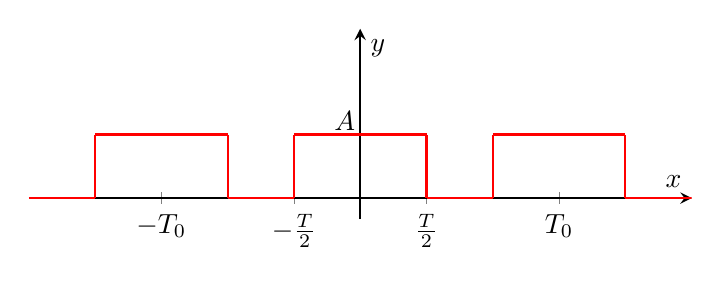
\begin{tikzpicture}
                        \begin{axis}[
                            xlabel=$x$,
                            ylabel=$y$,
                            xmin=-5,
                            xmax=5,
                            ymin=-0.5,
                            ymax=4,
                            ytick = {1.5},
                            xtick={-3,-1, 0, 1,3},
                            xticklabels={$-T_0$,$-\frac{T}{2}$, $0$, $\frac{T}{2}$,$T_0$},
                            yticklabels = {$A$},
                            yticklabel style = {yshift=5pt,xshift=4pt}, 
                            axis lines=middle,
                            thick,
                            domain=-5:5,
                            samples=100,
                            width=10cm,
                            height=4cm
                        ]
                        \addplot [const plot,red, thick] coordinates{(-1,1.5)(1,1.5)};
                        \addplot [const plot,red, thick] coordinates{(-1,0)(-1,1.5)};
                        \addplot [const plot,red, thick] coordinates{(1,0)(1,1.5)};
                        
                        \addplot [const plot,red, thick] coordinates{(-2,1.5)(-4,1.5)};
                        \addplot [const plot,red, thick] coordinates{(-2,0)(-2,1.5)};
                        \addplot [const plot,red, thick] coordinates{(-4,0)(-4,1.5)};
                        
                        \addplot [const plot,red, thick] coordinates{(2,1.5)(4,1.5)};
                        \addplot [const plot,red, thick] coordinates{(2,0)(2,1.5)};
                        \addplot [const plot,red, thick] coordinates{(4,0)(4,1.5)};
                        
                        \addplot [const plot,red, thick] coordinates{(2,0)(1,0)};
                        \addplot [const plot,red, thick] coordinates{(-2,0)(-1,0)};
                        \addplot [const plot,red, thick] coordinates{(-4,0)(-5,0)};
                        \addplot [const plot,red, thick] coordinates{(4,0)(5,0)};
                    
                        \end{axis}
                    \end{tikzpicture}
                    \caption{Treno di $A\hspace{0.1cm}rect\left(\frac{t}{T}\right)$}
                    \label{fig:treno di rect}
                \end{figure}                
                $\rightarrow$ Si nota come cambiare il periodi delle funzioni possiamo renderle da aperiodiche a periodiche e viceversa
                \begin{align}
                    ATSF[x_{(t)}] & = ATSF[\sum_{-\infty}^{\infty} x_R (t-nT_0)] \nonumber \\
                        & = \frac{1}{T_0} \int_{-\frac{T_0}{2}}^{\frac{T_0}{2}} x_{(t)} e^{-j2\pi kf_0t} dt = \frac{1}{T_0} \int_{-\frac{T}{2}}^{\frac{T}{2}} x_{(t)} e^{-j2\pi kf_0t} dt \nonumber \\
                        & = \frac{A}{T_0} \int_{-\frac{T}{2}}^{\frac{T}{2}} e^{-j2\pi kf_0t} dt = \eval{\frac{A}{T_0} \frac{1}{j2\pi kf_0} e^{-j2\pi kf_0t}}_{-\frac{T}{2}}^{\frac{T}{2}} \nonumber \\
                        & = \frac{A}{T_0} \frac{e^{-j\pi kf_0T} - e^{j\pi kf_0T}}{j2\pi kf_0} = \frac{A}{T_0} \frac{e^{j\pi kf_0T}-e^{-j\pi kf_0T}}{-j2\pi kf_0} \nonumber \\
                        & = \frac{A\color{purple}{T}}{T_0} \frac{e^{j\pi kf_0T}-e^{-j\pi kf_0T}}{-j2\pi kf_0\color{purple}{T}} = Af_0T sinc(kf_0T) \nonumber 
                \end{align}
                Tracciamo lo spettro per $f_0T<1$:
                \begin{figure}[H]
                    \centering
                    \subfloat[Spettro di Ampiezza]{
                        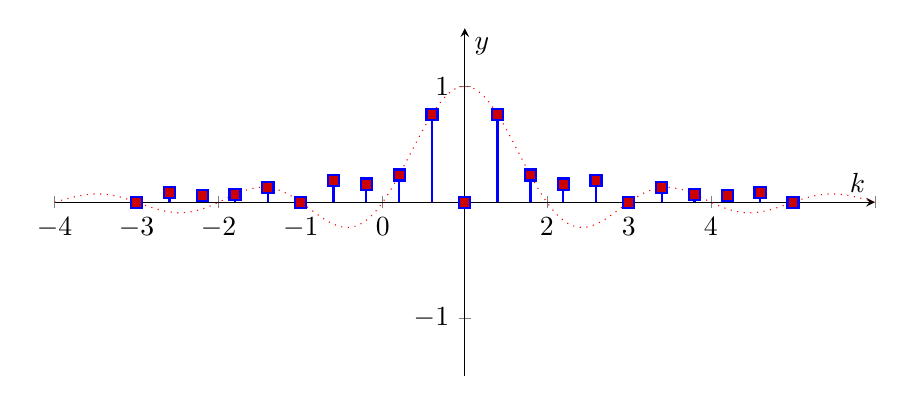
\begin{tikzpicture}
                            \begin{axis}[
                                domain=-5:5,
                                samples=200,
                                axis lines=middle,
                                xlabel=$k$,
                                ylabel=$y$,
                                ymin=-1.5,
                                ymax=1.5,
                                xtick={-5,-4,-3,-2,-1,0,1,2,3,4,5},
                                xticklabels={$-4$,$-3$,$-2$,$-1$,$0$,$1$,$2$,$3$,$4$},
                                ytick={-1, 1},
                                yticklabels={$-1$, $1$},
                                width=12cm,
                                height=6cm
                            ]
                            \addplot [red,dotted, samples = 300] {sin(deg(x*pi))/(x*pi)};
                            \addplot+ [blue, thick, ycomb, samples at={-4,-3.6,-3.2,-2.8,-2.4,-2,-1.6,-1.2,-0.8,-0.4,0,0.4,0.8,1.2,1.6,2,2.4,2.8,3.2,3.6,4}] {abs(sin(deg(x*pi))/(x*pi))};
                            \end{axis}
                        \end{tikzpicture}
                    }
                    \hfill
                    \subfloat[Spettro di Fase]{
                        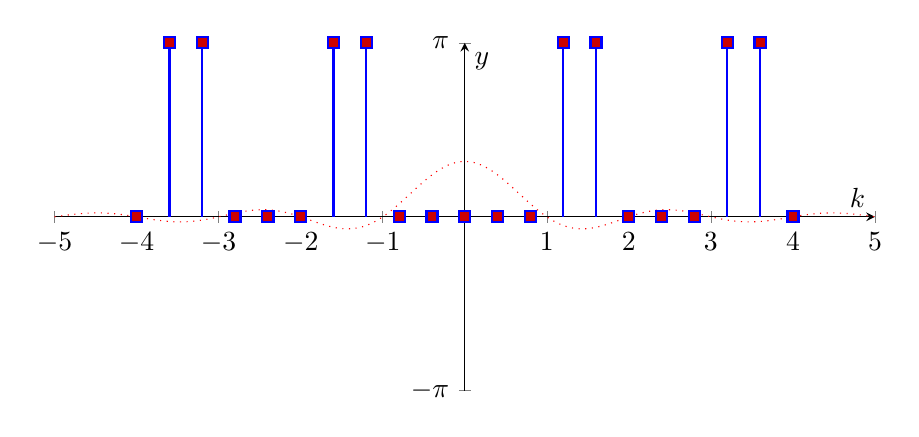
\begin{tikzpicture}
                            \begin{axis}[
                                domain=-5:5,
                                samples=200,
                                axis lines=middle,
                                xlabel=$k$,
                                ylabel=$y$,
                                ymin=-pi,
                                ymax=pi,
                                xtick={-5,-4,-3,-2,-1,0,1,2,3,4,5},
                                xticklabels={$-5$,$-4$,$-3$,$-2$,$-1$,$0$,$1$,$2$,$3$,$4$,$5$},
                                ytick={-pi, pi},
                                yticklabels={$-\pi$, $\pi$},
                                width=12cm,
                                height=6cm
                            ]
                            \addplot [red,dotted, samples = 300] {sin(deg(x*pi))/(x*pi)};
                            \addplot+ [blue, thick, ycomb, samples at={-4,-3.6,-3.2,-2.8,-2.4,-2,-1.6,-1.2,-0.8,-0.4,0,0.4,0.8,1.2,1.6,2,2.4,2.8,3.2,3.6,4}] {rad(atan2(0,sin(deg(x*pi))/(x*pi)))};
                            \end{axis}
                        \end{tikzpicture}
                    }
                    \caption{Spettro TSF del treno di rect con $f_0T<1$}
                \end{figure}
                Si possono anche unire i due spettri per ottenere: 
                \begin{figure}[H]
                    \centering
                    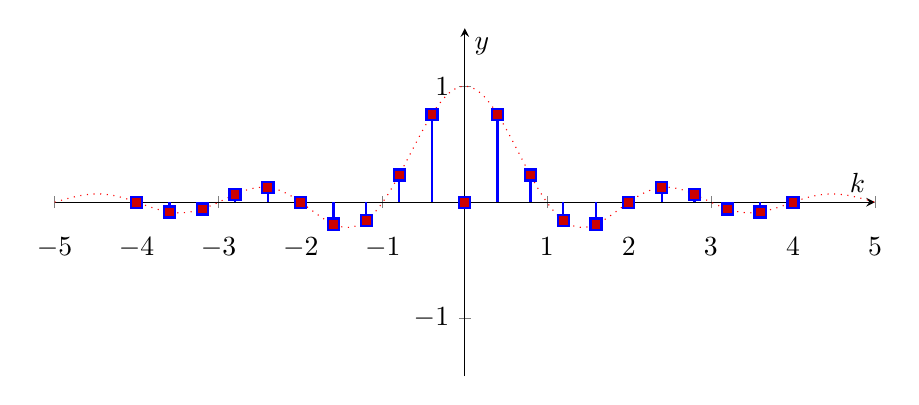
\begin{tikzpicture}
                        \begin{axis}[
                            domain=-5:5,
                            samples=200,
                            axis lines=middle,
                            xlabel=$k$,
                            ylabel=$y$,
                            ymin=-1.5,
                            ymax=1.5,
                            xtick={-5,-4,-3,-2,-1,0,1,2,3,4,5},
                            xticklabels={$-5$,$-4$,$-3$,$-2$,$-1$,$0$,$1$,$2$,$3$,$4$,$5$},
                            ytick={-1, 1},
                            yticklabels={$-1$, $1$},
                            xticklabel style = {yshift=-7pt}, 
                            width=12cm,
                            height=6cm
                        ]
                        \addplot [red,dotted, samples = 300] {sin(deg(x*pi))/(x*pi)};
                        \addplot+ [blue, thick, ycomb, samples at={-4,-3.6,-3.2,-2.8,-2.4,-2,-1.6,-1.2,-0.8,-0.4,0,0.4,0.8,1.2,1.6,2,2.4,2.8,3.2,3.6,4}] {sin(deg(x*pi))/(x*pi)};
                        \end{axis}
                    \end{tikzpicture}
                    \caption{Spettro treno di $A\hspace{0.1cm}rect\left(\frac{t}{T}\right)$}
                    \label{fig:Spettro treno di rect}
                \end{figure}  
            Ora appizza matlab e fa esempi di un segnale e uno di ricostruzione dello stesso(script di matlab presenti nel teams):
            \begin{itemize}
                \item Se un segnale varia molto rapidamente nel tempo ha componenti frequenziali piú alte $\rightarrow$ copre piú spettro(espansione spettrale) $T_0 \Downarrow$
                \item Se un segnale varia molto lentamente copre le basse fraquenze $ T_0 \Uparrow$
            \end{itemize}
            Se non ho abbastanza passi K non posso campionare le alte frequenze e quindi non faccio ne un analisi completa del segnale né riesco a ricostruire perfettamente il segnale  
            Inoltre in $0$ dello spettro ho il Valor medio \ref{Valore medio} del segnale.
    \section{Trasformata Continua Di Fourier}
    \subsection{Segnali Aperiodici}
        Nel caso di segnali come $x_{(t)}=rect\left(\frac{t}{T}\right)$ non posso usare la $TSF$ posso peró scrivere:
        \[
            x_{(t)} = \lim_{T_0\rightarrow\infty} x_p(t) ,\ x_p(t) = \sum_{n = -\infty}^{\infty} x_{(t-nT_0)} 
        \]
        Passiamo da un analisi a frequenze discrete ad un analisi su tutto lo spettro delle frequenze
        \begin{figure}[H]
            \centering
            \subfloat[Spettro di Ampiezza TSF]{
                    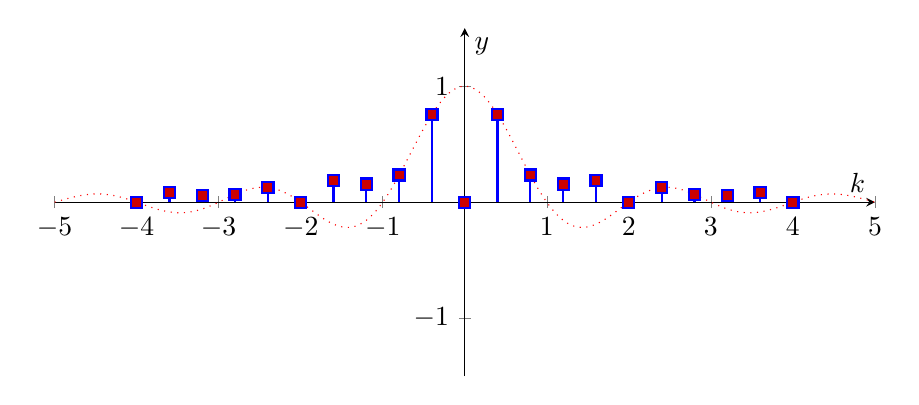
\begin{tikzpicture}
                        \begin{axis}[
                            domain=-5:5,
                            samples=200,
                            axis lines=middle,
                            xlabel=$k$,
                            ylabel=$y$,
                            ymin=-1.5,
                            ymax=1.5,
                            xtick={-5,-4,-3,-2,-1,0,1,2,3,4,5},
                            xticklabels={$-5$,$-4$,$-3$,$-2$,$-1$,$0$,$1$,$2$,$3$,$4$,$5$},
                            ytick={-1, 1},
                            yticklabels={$-1$, $1$},
                            width=12cm,
                            height=6cm
                        ]
                        \addplot [red,dotted, samples = 500] {sin(deg(x*pi))/(x*pi)};
                        \addplot+ [blue, thick, ycomb, samples at={-4,-3.6,-3.2,-2.8,-2.4,-2,-1.6,-1.2,-0.8,-0.4,0,0.4,0.8,1.2,1.6,2,2.4,2.8,3.2,3.6,4}] {abs(sin(deg(x*pi))/(x*pi))};
                        \end{axis}
                    \end{tikzpicture}
                }
                \hfill
                \subfloat[Spettro di Ampiezza TCF]{
                    \begin{tikzpicture}
                        \begin{axis}[
                            domain=-5:5,
                            samples=200,
                            axis lines=middle,
                            xlabel=$f$,
                            ylabel=$y$,
                            ymin=-1.5,
                            ymax=1.5,
                            xtick={-5,-4,-3,-2,-1,0,1,2,3,4,5},
                            xticklabels={$-5$,$-4$,$-3$,$-2$,$-1$,$0$,$1$,$2$,$3$,$4$,$5$},
                            ytick={-1, 1},
                            yticklabels={$-1$, $1$},
                            width=12cm,
                            height=6cm
                        ]
                        \addplot [red,dotted, samples = 300] {sin(deg(x*pi))/(x*pi)};
                        \addplot [blue, thick, samples = 300] {abs(sin(deg(x*pi))/(x*pi))};
                    \end{axis}
                    \end{tikzpicture}
                }
        \end{figure}

    \subsection{Equazioni di Analisi e Sintesi}
        \begin{figure}[H]
            \centering
            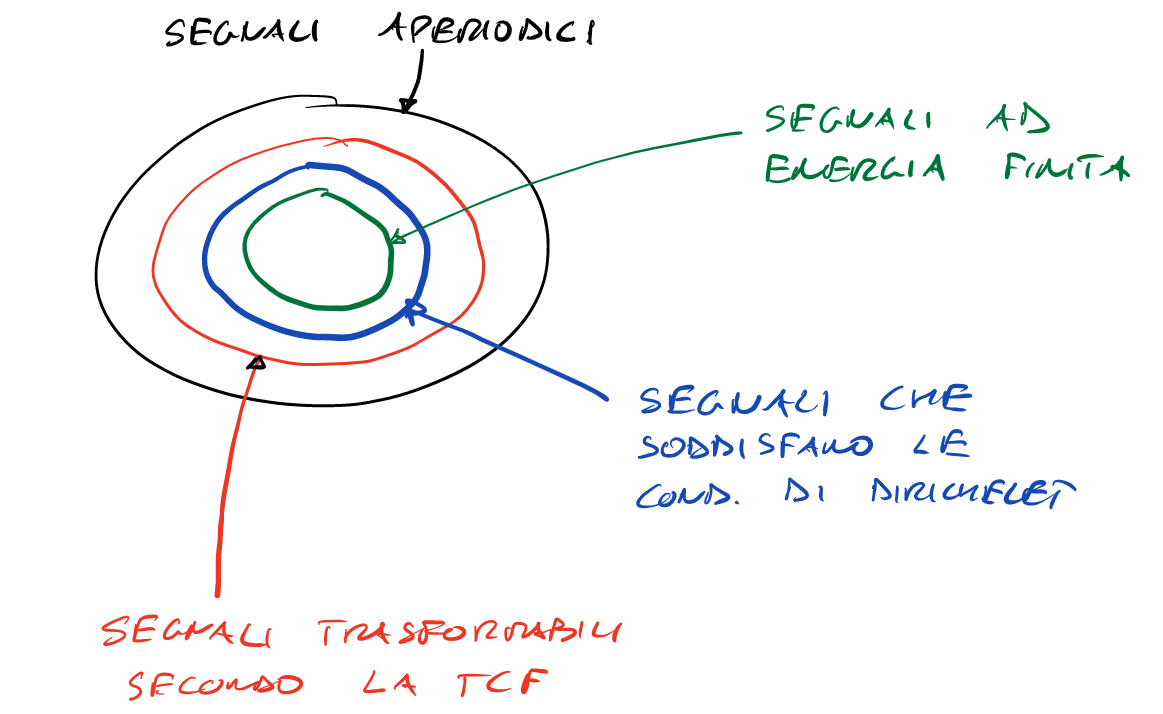
\includegraphics[width=12cm]{media/insiemi_tcf.png}
            \caption{Insiemi dei segnali per tcf}
            \label{fig:segnali aperiodici tcf}
        \end{figure}
        {\subsubsection{Equazione di Analisi}
            \[X_{(f)} = \int_{-\infty}^{\infty} x_{(t)} e^{-j2\pi ft} dt\hspace{0.3cm} Equazione\ di\ analisi \]
            
        \subsubsection{Equazione di Sintesi}
            \[x_{(t)} = \int_{-\infty}^{\infty} X_{(f)} e^{j2\pi ft} df\hspace{0.3cm} Equazione\ di\ sintesi \]
        }
        La $TCF$ gode della biunivocitá
        \begin{align}
            x_{(t)} \overunderset{TCF}{ATCF}{\leftrightharpoons}  X_{(f)}\nonumber \hspace{0.3cm} X_{(f)} \in \mathbb{C}
        \end{align}
        Essendo $X_{(f)}$ un numero complesso puó essere rappresentato in forma polare: 
        \[
            X_{(f)} = |X_{(f)}|e^{\angle X_{(f)}}  
        \]
        Si possono rappresentare il modulo (Ampiezza) e la fase tramite grafici che prendono il nome di spettri:
        \begin{figure}[H]
            \centering
            \subfloat[Spettro di Ampiezza]{
                    \begin{tikzpicture}
                        \begin{axis}[
                            domain=-5:5,
                            samples=200,
                            axis lines=middle,
                            xlabel=$f$,
                            ylabel=$y$,
                            ymin=-1.5,
                            ymax=1.5,
                            xtick={-5,-4,-3,-2,-1,0,1,2,3,4,5},
                            xticklabels={$-5$,$-4$,$-3$,$-2$,$-1$,$0$,$1$,$2$,$3$,$4$,$5$},
                            ytick={-1, 1},
                            yticklabels={$-1$, $1$},
                            width=12cm,
                            height=6cm
                        ]
                        \addplot [red,dotted, samples = 300] {sin(deg(x*pi))/(x*pi)};
                        \addplot [blue, thick, samples = 300] {abs(sin(deg(x*pi))/(x*pi))};
                    \end{axis}
                    \end{tikzpicture}
                }
            \hfill
            \subfloat[Spettro di Fase]{
                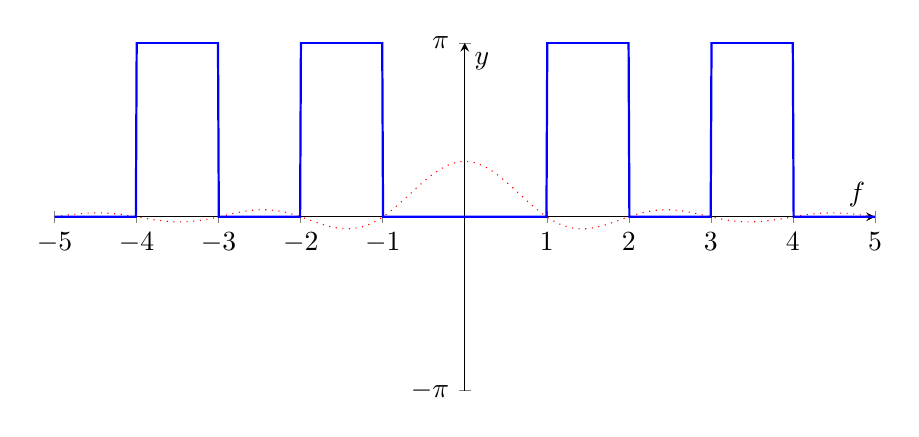
\begin{tikzpicture}
                    \begin{axis}[
                        domain=-5:5,
                        samples=200,
                        axis lines=middle,
                        xlabel=$f$,
                        ylabel=$y$,
                        ymin=-pi,
                        ymax=pi,
                        xtick={-5,-4,-3,-2,-1,0,1,2,3,4,5},
                        xticklabels={$-5$,$-4$,$-3$,$-2$,$-1$,$0$,$1$,$2$,$3$,$4$,$5$},
                        ytick={-pi, pi},
                        yticklabels={$-\pi$, $\pi$},
                        width=12cm,
                        height=6cm
                    ]
                    \addplot [red,dotted, samples = 300] {sin(deg(x*pi))/(x*pi)};
                    \addplot [blue, thick, samples = 1000] {rad(atan2(0,sin(deg(x*pi))/(x*pi)))};
                    \end{axis}
                \end{tikzpicture}
            }
            \caption{Spettro del segnale TCF}
        \end{figure}
        lo spettro di Ampiezza gode della \textbf{simmetria pari} rispetto alle ascisse quindi é \textbf{sempre positivo e continuo}, mentre lo spettro di fase della \textbf{simmetria dispari}, 
        questa propietá é chiamata \textbf{Simmetria Hermitiana}

        \subsubsection{TCF di una $Arect\left(\frac{t}{T}\right)$}
            $x_{(t)} = A\hspace{0.1cm}rect\left(\frac{t}{T}\right)$
            \begin{figure}[H]
                \centering
                \begin{tikzpicture}
                    \begin{axis}[
                        xlabel=$x$,
                        ylabel=$y$,
                        xmin=-5,
                        xmax=5,
                        ymin=-0.5,
                        ymax=4,
                        ytick = {1.5},
                        xtick={-1.5, 0, 1.5},
                        xticklabels={$-\frac{T}{2}$, $0$, $\frac{T}{2}$},
                        yticklabels = {$A$},
                        yticklabel style = {yshift=5pt,xshift=4pt}, 
                        axis lines=middle,
                        thick,
                        domain=-5:5,
                        samples=100,
                        width=8cm,
                        height=4cm
                    ]
                    \addplot [const plot,red, thick] coordinates{(-1.5,1.5)(1.5,1.5)};
                    \addplot [const plot,red, thick] coordinates{(-1.5,0)(-1.5,1.5)};
                    \addplot [const plot,red, thick] coordinates{(1.5,0)(1.5,1.5)};
                    \addplot [const plot,red, thick] coordinates{(5,0)(1.5,0)};
                    \addplot [const plot,red, thick] coordinates{(-5,0)(-1.5,0)};
                    \end{axis}
                  \end{tikzpicture}
                \caption{$A\hspace{0.1cm}rect\left(\frac{t}{T}\right)$}
                \label{fig:grafo rect nella tcf}
            \end{figure}
            $X_{(f)} = ? :$
            \begin{align}
                X_{(f)} & = \int_{-\infty}^{\infty} x_{(t)} e^{-j2\pi ft} dt \nonumber = \int_{-\frac{T}{2}}^{\frac{T}{2}} A\hspace{0.1cm}rect\left(\frac{t}{T}\right) e^{-j2\pi ft} dt \nonumber\\ 
                        & = A \int_{-\frac{T}{2}}^{\frac{T}{2}} e^{-j2\pi ft} dt = -\frac{A}{j2\pi f} \eval{e^{-j2\pi ft}}_{-\frac{T}{2}}^{\frac{T}{2}} =-\frac{A}{j2\pi f} \left(e^{-j\pi fT} - e^{j\pi fT}\right) \nonumber\\
                        & = \frac{A\color{purple}{T}}{\pi f} \left(\frac{e^{j\pi fT} - e^{-j\pi fT}}{2j}\right) = \frac{A{\color{purple}T}\sin(\pi fT)}{\pi f\color{purple}{T}} = AT sinc(fT) =  X_{(f)} \nonumber 
            \end{align}
            \[
                A\hspace{0.1cm}rect\left(\frac{t}{T}\right) \overunderset{TCF}{ATCF}{\leftrightharpoons} AT sinc(fT)
            \]
            La sinc si annulla in $\frac{k}{T},\ k\in \mathbb{Z}$. Notiamo anche come la funzione di partenza sia reale e pari la TCF rispetti \ref{Parita}:
            \begin{figure}[H]
                \centering

            \subfloat[Spettro di Ampiezza]{
                \begin{tikzpicture}
                    \begin{axis}[
                        domain=-5:5,
                        samples=200,
                        axis lines=middle,
                        xlabel=$f$,
                        ylabel=$y$,
                        ymin=-1.5,
                        ymax=1.5,
                        xtick={-5,-4,-3,-2,-1,0,1,2,3,4,5},
                        xticklabels={$-\frac{5}{T}$,$-\frac{4}{T}$,$-\frac{3}{T}$,$-\frac{2}{T}$,$-\frac{1}{T}$,$0$,$\frac{1}{T}$,$\frac{2}{T}$,$\frac{3}{T}$,$\frac{4}{T}$,$\frac{5}{T}$},
                        ytick={-1, 1},
                        yticklabels={$-1$, $1$},
                        width=12cm,
                        height=6cm
                    ]
                    \addplot [red,dotted, samples = 300] {sin(deg(x*pi))/(x*pi)};
                    \addplot [blue, thick, samples = 300] {abs(sin(deg(x*pi))/(x*pi))};
                \end{axis}
                \end{tikzpicture}
                }
            \hfill
            \subfloat[Spettro di Fase]{
                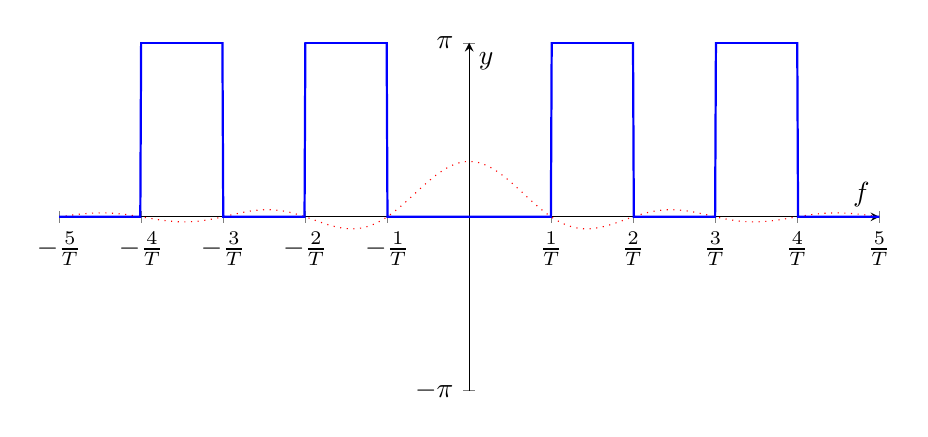
\begin{tikzpicture}
                    \begin{axis}[
                        domain=-5:5,
                        samples=200,
                        axis lines=middle,
                        xlabel=$f$,
                        ylabel=$y$,
                        ymin=-pi,
                        ymax=pi,
                        xtick={-5,-4,-3,-2,-1,0,1,2,3,4,5},
                        xticklabels={$-\frac{5}{T}$,$-\frac{4}{T}$,$-\frac{3}{T}$,$-\frac{2}{T}$,$-\frac{1}{T}$,$0$,$\frac{1}{T}$,$\frac{2}{T}$,$\frac{3}{T}$,$\frac{4}{T}$,$\frac{5}{T}$},
                        ytick={-pi, pi},
                        yticklabels={$-\pi$, $\pi$},
                        width=12cm,
                        height=6cm
                    ]
                    \addplot [red,dotted, samples = 300] {sin(deg(x*pi))/(x*pi)};
                    \addplot [blue, thick, samples = 1000] {rad(atan2(0,sin(deg(x*pi))/(x*pi)))};
                    \end{axis}
                \end{tikzpicture}
            }
            \end{figure}

    \subsection{Propietá}
        Come per la TSF vale che al variare del periodo della funzione $T$:
            \begin{itemize}
                \item Se $T\uparrow$ aumenta $ \rightarrow f\downarrow$ diminuisce e si stringe lo spettro  
                \item Se $T\downarrow$ diminuisce $ \rightarrow f\uparrow$ aumenta e si allarga lo spettro  
            \end{itemize}
        Inoltre come si puó evincere dal successivo Teorema della Dualitá \ref{Dualita}:
            \begin{itemize}
                \item Una funzione limitata (finita) nel tempo ha uno spettro nella frequenza illimitato $\rightarrow$ sono i segnali fisici   
                \item Una funzione illimitata nel tempo ha uno spettro nella frequenza limitato (finito)
            \end{itemize}
        Da come vedremo piú avanti quindi effettuare troncamenti in frequenza comporta, per alcuni segnali, perdere componenti ad alte
        frequenze, la scelta dell'intervallo di troncamento é cruciale per la ricostruzione del segnale: se tronchiamo un segnale perdendo
        le frequenze alte perdiamo le sue variazioni rapide, ad esempio se tronchiamo una $sinc(f)$ male potremmo non ottenere una buona $rect(t)$
        nel tempo.
        \subsubsection{Simmetria hermitiana}\label{Simmetria Hermitiana}
            \begin{align}
                Ip&: x_{(t)}\ reale \nonumber \\
                Th&: X_{(f)}\ hermitiana \nonumber \\ 
                X_{(-f)} &= X_{(f)}^{*} \rightarrow
                    \begin{cases}
                        |X_{(f)}| = |X_{(-f)}| \hspace{0.3cm} & Simmetria\ Pari \\
                        \angle X_{(-f)} = -\angle X_{(f)}\hspace{0.3cm} & Simmetria\ Dispari
                    \end{cases} \nonumber
            \end{align}

        \subsubsection{Paritá}\label{Parita}
            \begin{align}
                Ip&: x_{(t)}\ reale\ e\ pari  \nonumber \\
                Th&: X_{(f)}\ reale\ e\ pari \nonumber  
            \end{align}

        \subsubsection{Disparitá}\label{Disparita}
            \begin{align}
                Ip&: x_{(t)}\ reale\ e\ dispari  \nonumber \\
                Th&: X_{(f)}\ immaginaria\ e\ dispari \nonumber 
            \end{align}

    \subsection{Teoremi relativi alla TCF}
        \subsubsection{Linearitá}\label{Linearita}
            $Ip: x_{(t)} = \alpha x_{1(t)} + \beta x_{2(t)}$\\        
            $Th: X_{(f)} = \alpha X_{1(f)} + \beta X_{2(f)}$\\ 
            Dimostrazione:
            \begin{align}
                X_{(f)} & = \int_{-\infty}^{\infty} (\alpha x_{1(t)} + \beta x_{2(t)}) e^{-j2\pi ft} dt \nonumber \\
                        & = \alpha \int_{-\infty}^{\infty} x_{1(t)} e^{-j2\pi ft} dt + \beta \int_{-\infty}^{\infty}  x_{2(t)} e^{-j2\pi ft} dt  \nonumber \\
                        & = \alpha X_{1(f)} + \beta X_{2(f)} \nonumber
            \end{align}

            Esempio:
                {   
                    \begin{align}
                        x_{(t)} &= A rect\left(\frac{t}{2T}\right) + Brect\left(\frac{t}{T}\right)\nonumber \\   
                        X_{(f)} &= A X_{1(f)} + B X_{2(f)} = 2AT sinc(2Tf) + BT sinc(Tf) \nonumber \\
                        X_{1(f)} &= 
                        \begin{cases}
                            X_{1(f)} = A rect\left(\frac{t}{T^\prime}\right) \overset{TCF}{\leftrightharpoons} T^\prime sinc(T^\prime f) \Rightarrow X_{1(f)} =2Tsinc(2Tf) \\
                            T^\prime = 2T
                        \end{cases} \nonumber
                    \end{align}
                    \begin{figure}[H]
                        \centering
                        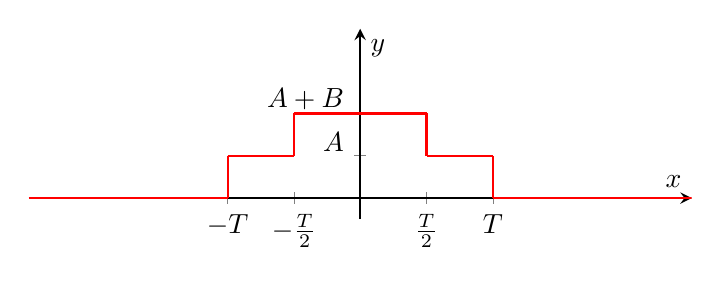
\begin{tikzpicture}
                            \begin{axis}[
                                xlabel=$x$,
                                ylabel=$y$,
                                xmin=-5,
                                xmax=5,
                                ymin=-0.5,
                                ymax=4,
                                ytick = {1,2},
                                yticklabels = {$A$,$A+B$},
                                xtick={-2,-1, 0, 1,2},
                                xticklabels={$-T$,$-\frac{T}{2}$, $0$, $\frac{T}{2}$,$T$},
                                yticklabel style = {yshift=5pt}, 
                                axis lines=middle,
                                thick,
                                domain=-5:5,
                                samples=100,
                                width=10cm,
                                height=4cm
                            ]
                            
                            \addplot [const plot,red, thick] coordinates{(-2,1)(-1,1)};
                            \addplot [const plot,red, thick] coordinates{(2,1)(1,1)};

                            \addplot [const plot,red, thick] coordinates{(1,1)(1,2)};
                            \addplot [const plot,red, thick] coordinates{(-1,1)(-1,2)};
                            \addplot [const plot,red, thick] coordinates{(-1,2)(1,2)};
                            
                            \addplot [const plot,red, thick] coordinates{(-2,0)(-2,1)};
                            \addplot [const plot,red, thick] coordinates{(2,0)(2,1)};


                            \addplot [const plot,red, thick] coordinates{(5,0)(2,0)};
                            \addplot [const plot,red, thick] coordinates{(-5,0)(-2,0)};
                            \end{axis}
                          \end{tikzpicture}
                        \caption{Segnale rettangolo}
                        \label{fig:es linearita}
                    \end{figure}                    
                }
                

        \subsubsection{Dualitá}\label{Dualita}
            $Ip: x_{(t)} \overunderset{TCF}{ATCF}{\leftrightharpoons} X_{(f)}$\\        
            $Th: X_{(t)} \overunderset{TCF}{ATCF}{\leftrightharpoons} x_{(-f)}$ \\
            Dimostrazione:
            \begin{align}
                X_{(f)} & = \int_{-\infty}^{\infty} x_{(t)} e^{-j2\pi ft} dt = Sost. \begin{cases}
                    t \rightarrow f\\
                    f \rightarrow t
                \end{cases} \Rightarrow  X_{(t)} = \int_{-\infty}^{\infty} x_{(f)} e^{-j2\pi tf} df \nonumber \\
                        & =Sost.\ (f^\prime = -f) \Rightarrow  X_{(t)} = \int_{-\infty}^{\infty} x_{(-f^\prime)} e^{-j2\pi t(-f^\prime)} df^\prime\nonumber \\
                        & =\int_{-\infty}^{\infty} x_{(-f^\prime)} e^{j2\pi tf^\prime} df^\prime= ACTF[x_{(-f)}] = c.v.d.  \nonumber
            \end{align}
            Esempio:\\
                {
                    $x_{(t)}=Asinc(Bt) \Rightarrow X_{(f)} = \int_{-\infty}^{\infty}A sinc(Bt)e^{-j2\pi ft}dt$ \\
                    Applico la dualitá:
                    \begin{gather}
                        A rect\left(\frac{t}{T}\right) \rightleftarrows ATsinc(Tf) \nonumber \\
                        ATsinc(Tt) \rightleftarrows A rect\left(\frac{-f}{T}\right) \nonumber
                    \end{gather}
                    Se voglio una durata generica:
                    \begin{gather}
                        Sostituisco\ B=T \nonumber \\
                        ABsinc(Bt) \rightleftarrows A rect\left(\frac{f}{B}\right) \nonumber  \\
                        \Downarrow \nonumber \\
                        Asinc(Bt) \rightleftarrows \frac{A}{B}rect\left(\frac{f}{B}\right) \nonumber
                    \end{gather}
                }

        \subsubsection{Ritardo}\label{Ritardo}
            $Ip: \begin{cases}
                x_{(t)} \overunderset{TCF}{ATCF}{\leftrightharpoons} X_{(f)} \nonumber \\
                y_{(t)} = x_{(t-to)} \nonumber
            \end{cases}$\\
            $Th: Y_{(f)} \overunderset{TCF}{ATCF}{\leftrightharpoons} y_{(t)} = X_{(f)}e^{-j2\pi ft_0}$\\ 
            Dimostrazione:
            \begin{align}
                Y_{(f)} & = \int_{-\infty}^{\infty} y_{(t)} e^{-j2\pi ft} dt = \int_{-\infty}^{\infty} x_{(t-t_0)} e^{-j2\pi tf} dt \nonumber \\
                        & =Sost.\ (t^\prime = t-t_0) \Rightarrow  Y_{(f)} = \int_{-\infty}^{\infty} x_{(t^\prime)} e^{-j2\pi f(t^\prime+t_0)} dt^\prime \nonumber \\
                        & =\int_{-\infty}^{\infty} x_{(t^\prime)} e^{-j2\pi ft^\prime}e^{-j2\pi ft_0} dt^\prime= X_{(f)}e^{-j2\pi ft_0}\ c.v.d.  \nonumber
            \end{align}
            {\em Osservazione:}
                \begin{itemize}
                    \item Un ritardo nel tempo introduce una componente solo di fase che cresce lienarmente con la frequenza
                    \item Un esponenziale nel tempo introduce un ritardo nel dominio della frequenza $x_{(t)}e^{-j2\pi f_0t} \rightarrowtail X_{(f-f_0)}$, vedi \ref{Modulazione con Esponenziale Complesso}
                \end{itemize}
            Esempio:\\
                {
                    $x_{0(t)} = A rect\left(\frac{t}{T}\right) \rightarrow x_{(t)}=x_{0(t-t_0)}\hspace{0.3cm} t_0 = \frac{T}{2}$
                    \begin{figure}[H]
                        \centering
                        \begin{tikzpicture}
                            \begin{axis}[
                                xlabel=$t$,
                                ylabel=$y$,
                                xmin=-5,
                                xmax=5,
                                ymin=-0.5,
                                ymax=4,
                                ytick = {1.5},
                                yticklabels = {$A$},
                                yticklabel style = {yshift=8pt,xshift=4pt}, 
                                xtick={-1,0,1,2},
                                xticklabels={$-\frac{T}{2}$,$0$,$\frac{T}{2}$,$T$},
                                axis lines=middle,
                                thick,
                                domain=-5:5,
                                samples=100,
                                width=10cm,
                                height=5cm
                            ]
                            
                            \addplot [const plot, blue] coordinates{(-1,1.5)(1,1.5)};
                            \addplot [const plot, blue] coordinates{(-1,0)(-1,1.5)};
                            \addplot [const plot, blue] coordinates{(1,0)(1,1.5)};
                            
                            \addplot [const plot, purple] coordinates{(0,1.5)(2,1.5)};
                            \addplot [const plot, purple] coordinates{(0,0)(0,1.5)};
                            \addplot [const plot, purple] coordinates{(2,0)(2,1.5)};
                            
                            \end{axis}
                        \end{tikzpicture}
                        \caption{{\color{blue}$x_{0(t)}$}, {\color{purple}$x_{(t)}$}}
                        \label{fig:ritardo rect}
                    \end{figure}
                    \[
                        X_{(f)} = X_{0(f)}e^{-j2\pi f\frac{T}{2}} = AT sinc(Tf) e^{-j\pi fT}    
                    \]

                    \begin{figure}[H]
                        \centering
                        \subfloat[Ampiezza con ritardo]{
                            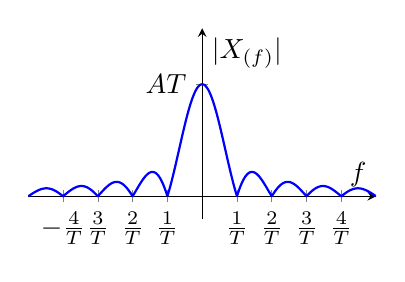
\begin{tikzpicture}
                                \begin{axis}[
                                    domain=-5:5,
                                    samples=200,
                                    axis lines=middle,
                                    xlabel=$f$,
                                    ylabel=$|X_{(f)}|$,
                                    ytick = {1},
                                    yticklabels = {$AT$},
                                    xtick = {-4,-3,-2,-1,0,1,2,3,4},
                                    xticklabels = {$-\frac{4}{T}$,$\frac{3}{T}$,$\frac{2}{T}$,$\frac{1}{T}$,$0$,$\frac{1}{T}$,$\frac{2}{T}$,$\frac{3}{T}$,$\frac{4}{T}$},
                                    ymin=-0.2,
                                    ymax=1.5,
                                    width=6cm,
                                    height=4cm
                                ]
                                \addplot [blue, thick, samples = 500] {abs(sin(deg(x*pi))/(x*pi))};
                                \end{axis}
                            \end{tikzpicture}
                            \label{fig:Ampiezza}
                        }
                        \hfill
                        \subfloat[Fase con ritardo]{
                                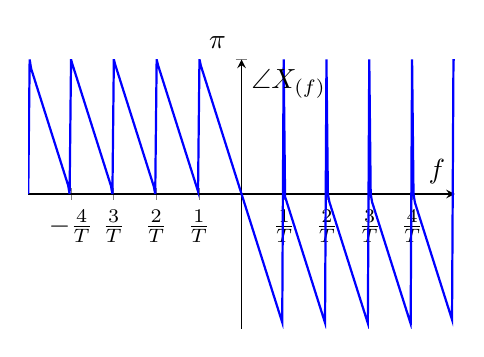
\begin{tikzpicture}
                                    \begin{axis}[
                                        domain=-5:5,
                                        samples=200,
                                        axis lines=middle,
                                        xlabel=$f$,
                                        ylabel=$\angle X_{(f)}$,
                                        ymin=-pi,
                                        ymax=pi,
                                        xtick = {-4,-3,-2,-1,0,1,2,3,4},
                                        xticklabels = {$-\frac{4}{T}$,$\frac{3}{T}$,$\frac{2}{T}$,$\frac{1}{T}$,$0$,$\frac{1}{T}$,$\frac{2}{T}$,$\frac{3}{T}$,$\frac{4}{T}$},
                                        ytick={pi},
                                        yticklabel style = {yshift=6pt}, 
                                        yticklabels={$\pi$},
                                        width=7cm,
                                        height=5cm
                                    ]
                                    \addplot [blue, thick, samples = 300] {rad(atan2((-((sin(deg(pi*x)))^2)/(pi*x)),((cos(deg(pi*x))*sin(deg(pi*x)))/(pi*x))))};
                                    \end{axis}
                                \end{tikzpicture}
                            \label{fig:fase}
                        }
                        \caption{Spettro della $rect$ con ritardo}
                    \end{figure}
                    Il \LaTeX{} sbaglia e aggiunge le spike nelle $f$ positive, il grafico é dispari con andamento come per le $f$ negative.
                }

        \subsubsection{Derivazione}\label{Derivazione}
            $Ip:\begin{cases}
                x_{(t)}\overunderset{TCF}{ATCF}{\leftrightharpoons} X_{(f)}\\
                y_{(t)}= \derivative{}{t} x_{(t)}        
            \end{cases}$\\
            $Th: Y_{(f)} = j2\pi f X_{(f)} $ \\
            Dimostrazione:\\
            \begin{align}
                y_{(t)} &= \derivative{}{t} x_{(t)} = \derivative{}{t} ACTF[x_{(t)}] =\derivative{}{t} \int_{-\infty}^{\infty} X_{(f)}e^{j2\pi ft} df = \nonumber\\
                        &= \int_{-\infty}^{\infty} X_{(f)}\derivative{}{t}e^{j2\pi ft} df = \int_{-\infty}^{\infty} X_{(f)}j2\pi fe^{j2\pi ft} df \nonumber
            \end{align}
            Posso Scrivere $y_{(t)}$ come $ACTF[y_{(t)}] = \int_{-\infty}^{\infty} Y_{(f)}e^{j2\pi ft} df $, se quindi $Y_{(f)} = j2\pi f X_{(f)}$ l'ugaglianza é valida:
            \[
                y_{(t)} =\int_{-\infty}^{\infty} Y_{(f)}e^{j2\pi ft} df
            \]
            L'operazione di derivata nel dominio della frequenza si traduce in una semplice operazione algebrica, nel tempo avrei dovuto calcolare il 
            rapporto incrementale. Per derivare un segnale posso quindi:
            \begin{gather}
                x_{(t)} \rightarrow TCF \rightarrow j2\pi fX_{(f)} \rightarrow ACTF \rightarrow y_{(t)}\nonumber
            \end{gather}
            
        \subsubsection{Integrazione}\label{Integrazione}
            $Ip:\begin{cases}
                x_{(t)} \overunderset{TCF}{ATCF}{\leftrightharpoons} X_{(f)}\ (1)\\
                y_{(t)} = \int_{-\infty}^{t} x_{(\alpha)} d\alpha\ (2) \\
                \int_{-\infty}^{\infty} x_{(t)} dt\ oppure\ \eval*{X_{(f)}}_{f=0} = 0 \ oppure\ y{(+\infty)} = 0\ (3) \\
            \end{cases}$\\
            $Th: Y_{(f)} =\frac{X_{(f)}}{j2\pi f}$ \\
            Dimostrazione:\\
            \begin{gather}
                y_{(t)} = \int_{-\infty}^{t} x_{(\alpha)} d\alpha \Rightarrow {\color{purple}\derivative{}{t}} x_{(t)} = {\color{purple}\derivative{}{t}} y_{(t)} \overset{Th. \ref{Derivazione}}{\Rightarrow}  X_{(f)} = j2\pi f Y_{(f)} \nonumber\\
                         Y_{(f)} =\frac{X_{(f)}}{j2\pi f}\nonumber
            \end{gather}

            L'ipotesi 3 é conseguenza della divisione per $f$ e che devo mantenere l'uguaglianza $X_{(f)} = j2\pi f Y_{(f)}$, si nota come nella dimostrazione usando il Th della Derivazione (\ref{Derivazione})
            quando $f=0$ la funzione nella frequenza deve essere $0,\ X_{(f)} = j2\pi f Y_{(f)} = 0$ 
        
        Esempio: $TCF$ di una piramide\\
        {
            \[
                x_{(t)} = A\left(1-\left(\frac{|t|}{T}\right)\right)rect \left(\frac{t}{2T}\right) \hspace{0.3cm} X_{(f)} = TCF[x_{(t)}] = ?
            \]
            \begin{figure}[H]
                \centering
                \begin{tikzpicture}
                    \begin{axis}[
                        xlabel=$t$,
                        ylabel=$x_{(t)}$,
                        xmin=-5,
                        xmax=5,
                        ymin=-0.5,
                        ymax=3,
                        ytick = {2},
                        yticklabels = {$A$},
                        xtick={-2,0,2},
                        xticklabels={$-T$,$0$,$T$},
                        axis lines=middle,
                        thick,
                        domain=-5:5,
                        samples=100,
                        width=10cm,
                        height=5cm
                    ]
                    
                    \addplot [sharp plot, blue] coordinates{(-2,0)(0,2)};
                    \addplot [sharp plot, blue] coordinates{(2,0)(0,2)};
                    \addplot [sharp plot, blue] coordinates{(2,0)(5,0)};
                    \addplot [sharp plot, blue] coordinates{(-2,0)(-5,0)};

                    \end{axis}
                \end{tikzpicture}
                \caption{Funzione priamide}
                \label{fig:funzione piramide}
            \end{figure}
            $TCF[x_{(t)}]:$
            \begin{itemize}
                \item {
                    Utilizzando la classica $TCF$:\\     
                        \[X_{(f)} = \int_{-\infty}^{\infty} A\left(1-\left(\frac{|t|}{T}\right)\right)rect \left(\frac{t}{2T}\right) dt\]
                }
                \item {
                    Utilizzando il Th dell'Integrazione \ref{Integrazione}:\\     
                    \begin{gather}
                        y_{(t)} = \derivative{}{t} x_{(t)} \implies x_{(t)}= \int_{-\infty}^{t} y_{(\alpha)} d\alpha\ \ref{Integrazione}(2) \nonumber \\
                        \int_{-\infty}^{\infty} y_{(t)} dt\ \ref{Integrazione}(3) \nonumber
                    \end{gather}
                    \begin{figure}[H]
                        \centering
                        \begin{tikzpicture}
                            \begin{axis}[
                                xlabel=$t$,
                                ylabel=$x_{(t)}$,
                                xmin=-5,
                                xmax=5,
                                ymin=-3,
                                ymax=3,
                                ytick = {-2,2},
                                yticklabels = {$-\frac{A}{T}$,$\frac{A}{T}$},
                                xtick={-2,-1,0,1,2},
                                xticklabels={$-T$,$-\frac{T}{2}$,$0$,$\frac{T}{2}$,$T$},
                                yticklabel style = {yshift=7pt}, 
                                axis lines=middle,
                                thick,
                                domain=-5:5,
                                samples=100,
                                width=10cm,
                                height=5cm
                            ]
                            
                            \addplot [sharp plot, blue] coordinates{(-2,0)(-2,2)};
                            \addplot [sharp plot, blue] coordinates{(-2,2)(0,2)};

                            \addplot [sharp plot, blue] coordinates{(0,2)(0,-2)};

                            \addplot [sharp plot, blue] coordinates{(0,-2)(2,-2)};
                            \addplot [sharp plot, blue] coordinates{(2,0)(2,-2)};
                            
                            \addplot [sharp plot, blue] coordinates{(-2,0)(-5,0)};
                            \addplot [sharp plot, blue] coordinates{(2,0)(5,0)};
        
                            \end{axis}
                        \end{tikzpicture}
                        \caption{Funzione priamide}
                        \label{fig:derivata piramide}
                    \end{figure}
                    \begin{align}
                        y_{(t)} &= \frac{A}{T}rect \left(\frac{t-\left(-\frac{T}{2}\right)}{T}\right) - \frac{A}{T}rect \left(\frac{t-\frac{T}{2}}{T}\right) = Sono\ 2\ rect\ con\ ritardo \nonumber \\
                                &\Rightarrow y_{(t)} \rightleftharpoons Y_{(f)}\ \ref{Integrazione} (1)\Rightarrow X_{(f)}=\frac{Y_{(f)}}{j2\pi f} 
                                \begin{cases}
                                    x_{(t-t_0)} \rightleftharpoons X_{(f)} e^{-j2\pi ft_0}\nonumber\\
                                    rect \left(\frac{t}{T}\right) \rightleftharpoons Tsinc(Tf) \nonumber
                                \end{cases}\nonumber \\
                        Y_{(f)} &= \frac{A}{T}Tsinc(Tf)e^{-j2\pi f\left(-\frac{T}{2}\right)} - \frac{A}{T}Tsinc(Tf)e^{-j2\pi f\frac{T}{2}} \nonumber\\
                                &= {\color{purple}2j}Asinc(Tf)\frac{e^{j\pi fT}-e^{j\pi fT}}{{\color{purple}2j}} = 2jAsinc(Tf)\sin(\pi fT) \nonumber \\
                        X_{(f)} &= \frac{Y_{(f)}}{j2\pi f} = \frac{2jAsinc(Tf)\sin(\pi fT)}{j2\pi f} = \frac{A{\color{purple}T}sinc(Tf)\sin(\pi fT)}{\pi f{\color{purple}T}}\nonumber\\
                                &= ATsinc^2(fT) \nonumber
                    \end{align}
                    Abbiamo ottenuto la $TCF$ del triangolo:
                    \begin{gather}
                        A\left(1-\left(\frac{|t|}{T}\right)\right)rect \left(\frac{t}{2T}\right) \rightleftharpoons ATsinc^2(fT)\nonumber\\
                        per\ la\ dualita \ref{Dualita}: \nonumber \\
                        ABsinc^2(Bt) \rightleftharpoons A\left(1-\left(\frac{|f|}{B}\right)\right)rect \left(\frac{f}{2B}\right) \nonumber
                    \end{gather} 
                    I segni negativi spariscono per il valore assoluto e per la paritá della $rect$. Per verificare che i calcoli siano
                    corretti posso colacolare la $X_{(f)}$ in $0$ e vedo quanto é l'area del segnale: 
                    \[
                        \eval{T^2sinc(Tf)}_{0} = T^2 \hspace{.2cm} \int_{-\infty}^{\infty} Trect(\frac{t}{T}) = T  
                    \]
                    {\em Osservazione}: la funzione piramidale varia meno rapidamente nel {\em tempo} rispetto alla funzione rettangolare
                    quindi lo spetto non occupa le alte frequenze, l'andamento é di $\frac{sinc^2}{x^2}$, é molto piú contenuto. La rect avendo un gradino
                    varia molto rapidamente nel {\em tempo} e di conseguenza il suo spettro si estende a frequenze piú alte del segnale priamidale.
                    \begin{figure}[H]
                        \centering
                        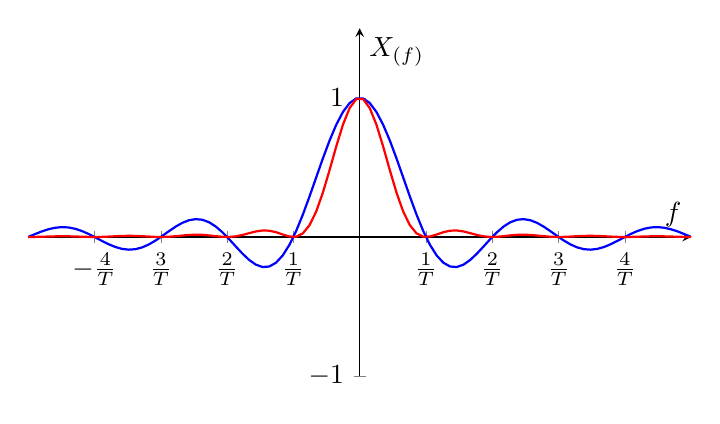
\begin{tikzpicture}
                            \begin{axis}[
                                domain=-5:5,
                                samples=200,
                                axis lines=middle,
                                xlabel=$f$,
                                ylabel=$X_{(f)}$,
                                ytick = {},
                                xtick = {-4,-3,-2,-1,0,1,2,3,4},
                                xticklabels = {$-\frac{4}{T}$,$\frac{3}{T}$,$\frac{2}{T}$,$\frac{1}{T}$,$0$,$\frac{1}{T}$,$\frac{2}{T}$,$\frac{3}{T}$,$\frac{4}{T}$},
                                ymin=-1,
                                ymax=1.5,
                                width=10cm,
                                height=6cm
                            ]
                            \addplot [blue, thick, samples = 100] {sin(deg(x*pi))/(x*pi)};
                            \addplot [red, thick, samples = 100] {(sin(deg(x*pi)))^2/(x*pi)^2};
                            \end{axis}
                        \end{tikzpicture}
                        \caption{{\color{blue}$\frac{sinc}{x}$}, {\color{red}$\frac{sinc^2}{x^2}$}}
                        \label{fig:sinc vs sinc2}
                    \end{figure}
                }
            \end{itemize}
        }
        
        \subsubsection{Derivazione in Frequenza}\label{Derivazione in Frequenza}
            $Ip:\begin{cases}
                x_{(t)}\overunderset{TCF}{ATCF}{\leftrightharpoons} X_{(f)}\\
                y_{(t)}= \derivative{x_{(t)}}{t}
            \end{cases}$\\
            $Th: Y_{(f)} = j2\pi f X_{(f)} $ \\
            
                
        \subsubsection{Integrazione in Frequenza}\label{Integrazione in Frequenza}
            $Ip:\begin{cases}
                x_{(t)}\overunderset{TCF}{ATCF}{\leftrightharpoons} X_{(f)} \\
                y_{(t)}= \derivative{x_{(t)}}{t}
            \end{cases}$\\
            $Th: Y_{(f)} = j2\pi f X_{(f)} $ \\
            

                        
        \subsubsection{Convoluzione}\label{Convoluzione}
            \[
                z_{(t)} = x_{(t)} \otimes  y_{(t)} \triangleq \int_{-\infty}^{\infty} x_{(\tau)}y_{(t-\tau)} d\tau
            \] 
            $Ip:\begin{cases}
                x_{(t)}\overunderset{TCF}{ATCF}{\leftrightharpoons} X_{(f)} \\
                x_{(t)}\overunderset{TCF}{ATCF}{\leftrightharpoons} X_{(f)} \\
                z_{(t)} = x_{(t)} \otimes  y_{(t)}   
            \end{cases}$\\
            $Th: Z_{(f)} = X_{(f)}Y_{(f)} $ \\
            Dimostrazione:
                \begin{align}
                    Z_{(f)} &= \int_{-\infty}^{\infty} z_{(t)} e^{-j2\pi ft} dt = \int_{-\infty_{t}}^{\infty}\int_{-\infty_{\tau}}^{\infty} x_{(\tau)}y_{(t-\tau)} e^{-j2\pi ft} dt\ d\tau \nonumber \\
                            &= \int_{-\infty_{t}}^{\infty}x_{(\tau)}\int_{-\infty_{\tau}}^{\infty} y_{(t-\tau)}e^{-j2\pi ft}  dt\ d\tau \overset{Th. \ref{Ritardo}}{\Rightarrow} \int_{-\infty}^{\infty}Y_{(f)}x_{(\tau)}e^{-j2\pi f\tau} d\tau  \nonumber \\
                            &= X_{(f)}Y_{(f)} \nonumber
                \end{align}
            Propietá della convoluzione:
            \begin{itemize}
                \item {
                        Commutativa:
                        \[
                            z_{(t)} = x_{(t)} \otimes  y_{(t)} = y_{(t)} \otimes  x_{(t)}  
                        \]
                        Dimostrazione:
                        \begin{align}
                            z_{(t)} &= \int_{-\infty}^{\infty} x_{(\tau)}y_{(t-\tau)} d\tau \Rightarrow \tau=t-\tau^\prime\Rightarrow \int_{-\infty}^{\infty} x_{(t-\tau^\prime)}y_{(\tau^\prime)} d\tau^\prime \nonumber \\
                                    &= \int_{-\infty}^{\infty} y_{(\tau^\prime)}x_{(t-\tau^\prime)} d\tau^\prime = y_{(t)} \otimes  x_{(t)}\nonumber 
                        \end{align}
                    }\label{Conv. Commutativa}
                \item {
                        Associativa:
                        \[
                            (x_{(t)} \otimes  y_{(t)}) \otimes z_{(t)}  =x_{(t)} \otimes  (y_{(t)} \otimes z_{(t)})   
                        \]
                    }\label{Conv. Distributiva}
                \item {
                        Distributiva:
                        \[
                            x_{(t)} \otimes  (y_{(t)}+z_{(t)}) = x_{(t)}\otimes  y_{(t)} +x_{(t)}\otimes  z_{(t)}  
                        \]
                        Dimostrazione:
                        \begin{align}
                            z_{(t)} &= \int_{-\infty}^{\infty} x_{(\tau)}(y_{(t-\tau)}+z_{(t-\tau)}) d\tau = \int_{-\infty}^{\infty}x_{(\tau)}y_{(t-\tau)} +x_{(\tau)}z_{(t-\tau)} d\tau \nonumber \\
                                    &= \int_{-\infty}^{\infty}x_{(\tau)}y_{(t-\tau)} d\tau +\int_{-\infty}^{\infty}x_{(\tau)}z_{(t-\tau)} d\tau = x_{(t)}\otimes  y_{(t)} +x_{(t)}\otimes  z_{(t)} \nonumber 
                        \end{align}
                    }\label{Conv. Associativa}
            \end{itemize}
            Tutte le propietá sono valutate nel dominio del $tempo$ ma valgono anche per il dominio della $frequenza$.
        \subsubsection{Prodotto}\label{Prodotto}
            $Ip:\begin{cases}
                x_{(t)}\overunderset{TCF}{ATCF}{\leftrightharpoons} X_{(f)} \\
                x_{(t)}\overunderset{TCF}{ATCF}{\leftrightharpoons} X_{(f)} \\
                z_{(t)} = x_{(t)}y_{(t)}   
            \end{cases}$\\
            $Th: Z_{(f)} = X_{(f)}\otimes Y_{(f)} $ \\
            Dimostrazione:
                \begin{align}
                    Z_{(f)} &= \int_{-\infty}^{\infty} z_{(t)} e^{-j2\pi ft} dt = \int_{-\infty}^{\infty}x_{(t)}y_{(t)} e^{-j2\pi ft} dt \nonumber \\
                            &= \int_{-\infty_{t}}^{\infty} \int_{-\infty_{\alpha}}^{\infty}X_{(\alpha)}e^{j2\pi \alpha t} d\alpha\ y_{(t)}e^{-j2\pi ft} dt =\int_{-\infty_{\alpha}}^{\infty}X_{(\alpha)} \int_{-\infty_{t}}^{\infty}y_{(t)}e^{-j2\pi (f-\alpha)t} dt\ d\alpha\nonumber \\
                            &\overset{Th. \ref{Ritardo}}{\Rightarrow} \int_{-\infty}^{\infty}X_{(\alpha)}Y_{(f-\alpha)}  d\alpha = X_{(f)}\otimes Y_{(f)} \nonumber 
                \end{align}
            \begin{align}
                Tempo&\hspace{1cm} Frequenza \nonumber \\ 
                Convoluzione\ &\Longleftrightarrow \ Prodotto \nonumber \\ 
                Prodotto\ &\Longleftrightarrow \ Convoluzione \nonumber 
            \end{align}
        \subsubsection{Calcolo del prodotto di convoluzione}\label{Calcolo del prodotto di convoluzione}
        \[
            x_{(t)} \otimes  y_{(t)} = \int_{-\infty}^{\infty} x_{(\tau)}y_{(t-\tau)} d\tau \hspace{1cm} y_{(-\tau)}\ e^\prime\ y_{(\tau)}\ ruotato 
        \]
        Facciamo un esempio con 2 $rect$:\\

        $x_{(t)} = y_{(t)} = rect\left(\frac{t}{T}\right)$
        \begin{figure}[H]
            \centering
            \subfloat[Grafico nel tempo,{\color{red}$y_{(-\alpha)}$},{\color{blue}$x_{(\alpha)}$}]{
                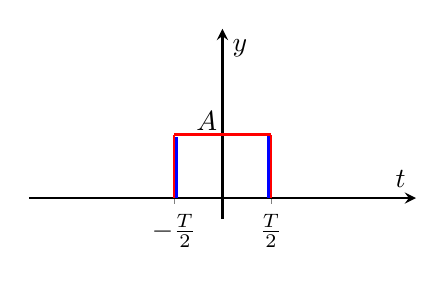
\begin{tikzpicture}
                    \begin{axis}[
                        xlabel=$t$,
                        ylabel=$y$,
                        xmin=-4,
                        xmax=4,
                        ymin=-0.5,
                        ymax=4,
                        ytick = {1.5},
                        xtick={-1, 0, 1},
                        xticklabels={$-\frac{T}{2}$, $0$, $\frac{T}{2}$},
                        yticklabels = {$A$},
                        yticklabel style = {yshift=5pt,xshift=4pt}, 
                        axis lines=middle,
                        thick,
                        domain=-4:4,
                        samples=100,
                        width=6.5cm,
                        height=4cm
                    ]
                    \addplot [const plot, blue, thick] coordinates{(-0.95,1.49)(0.95,1.45)};
                    \addplot [const plot, blue, thick] coordinates{(-0.95,0)(-0.95,1.45)};
                    \addplot [const plot, blue, thick] coordinates{(0.95,0)(0.95,1.45)};
                
                    \addplot [const plot, red, thick] coordinates{(-1,1.5)(1,1.5)};
                    \addplot [const plot, red, thick] coordinates{(-1,0)(-1,1.5)};
                    \addplot [const plot, red, thick] coordinates{(1,0)(1,1.5)};
                
                    \end{axis}
                \end{tikzpicture}
                \label{fig:PC rect}
            }
            \hfill
            \subfloat[illustrazione dell'integrale al variare di $t$,{\color{green}$y_{(t-\alpha)}$},{\color{blue}$x_{(\alpha)}$}]{
                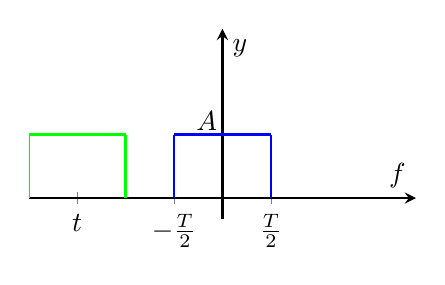
\begin{tikzpicture}
                    \begin{axis}[
                        xlabel=$f$,
                        ylabel=$y$,
                        xmin=-4,
                        xmax=4,
                        ymin=-0.5,
                        ymax=4,
                        ytick = {1.5},
                        xtick={-3,-1, 0, 1},
                        xticklabels={$t$,$-\frac{T}{2}$, $0$, $\frac{T}{2}$},
                        yticklabels = {$A$},
                        yticklabel style = {yshift=5pt,xshift=4pt}, 
                        axis lines=middle,
                        thick,
                        domain=-5:5,
                        samples=100,
                        width=6.5cm,
                        height=4cm
                    ]

                    \addplot [const plot, green, thick] coordinates{(-4,1.5)(-2,1.5)};
                    \addplot [const plot, green, thick] coordinates{(-4,0)(-4,1.5)};
                    \addplot [const plot, green, thick] coordinates{(-2,0)(-2,1.5)};

                    \addplot [const plot, blue, thick] coordinates{(-1,1.5)(1,1.5)};
                    \addplot [const plot, blue, thick] coordinates{(-1,0)(-1,1.5)};
                    \addplot [const plot, blue, thick] coordinates{(1,0)(1,1.5)};
                    \end{axis}
                \end{tikzpicture}
                \label{fig:PC rect in rect}
            }
            \caption{Grafico per il calcolo del prodotto di convoluzione}
        \end{figure}    
        All'aumentare di $t$ {\color{green}$y_{(t-\alpha)}$} si sposta sull'asse delle ascisse, se:
        \begin{itemize}
            \item {
                $t=-\frac{T}{2}$: si allineano le due $rect$ e il valore dell'integrale inizia a aumentare.
            }
            \item {
                $t=0$: si ha il valore massimo del prodotto tra le due funzioni (in questo caso $A=1$), l'integrale vale T.
            }
            \item {
                $t=\frac{T}{2}$: le due $rect$ sono disgiunte, nel raggiungere questa posizione il valore dell'integrale é diminuito fino a $0$.
            }
        \end{itemize}
        Traccamo l'andamento dell'integrale:
        \begin{figure}[H]
            \centering
            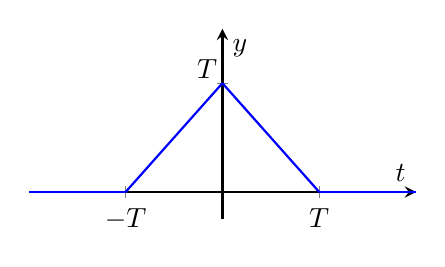
\begin{tikzpicture}
                \begin{axis}[
                    xlabel=$t$,
                    ylabel=$y$,
                    xmin=-4,
                    xmax=4,
                    ymin=-0.5,
                    ymax=3,
                    ytick = {2},
                    xtick={-2, 0, 2},
                    xticklabels={$-T$, $0$, $T$},
                    yticklabels = {$T$},
                    yticklabel style = {yshift=5pt,xshift=4pt}, 
                    axis lines=middle,
                    thick,
                    domain=-4:4,
                    samples=100,
                    width=6.5cm,
                    height=4cm
                ]
                \addplot [sharp plot, blue, thick] coordinates{(-2,0)(0,2)};
                \addplot [sharp plot, blue, thick] coordinates{(2,0)(0,2)};
            
                \addplot [const plot, blue, thick] coordinates{(-2,0)(-4,0)};
                \addplot [const plot, blue, thick] coordinates{(2,0)(4,0)};
            
                \end{axis}
            \end{tikzpicture}
            \label{fig:PC valore integrale}
            \caption{Integrale di convoluzione}
        \end{figure}

        {\em Osservazioni}:
        \begin{itemize}
            \item {Il prodotto di convoluzione ha come durata la somma delle durate dei segnali $[-\frac{T}{2},\frac{T}{2}]\rightarrow[-T,T]$}
            \item {In $t=0$ é l'area il prodotto dei segnali}
        \end{itemize}
        Esempio con $rect$ di durata $T$ e $2T$: 
        \begin{figure}[H]
            \centering
            \subfloat[Grafico delle rect]{
                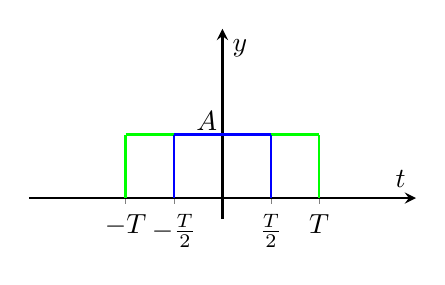
\begin{tikzpicture}
                    \begin{axis}[
                        xlabel=$t$,
                        ylabel=$y$,
                        xmin=-4,
                        xmax=4,
                        ymin=-0.5,
                        ymax=4,
                        ytick = {1.5},
                        xtick={-2,-1, 0, 1,2},
                        xticklabels={$-T$,$-\frac{T}{2}$, $0$, $\frac{T}{2}$,$T$},
                        yticklabels = {$A$},
                        yticklabel style = {yshift=5pt,xshift=4pt}, 
                        axis lines=middle,
                        thick,
                        domain=-4:4,
                        samples=100,
                        width=6.5cm,
                        height=4cm
                    ]
                 
                    \addplot [const plot, green, thick] coordinates{(-2,0)(-2,1.5)};
                    \addplot [const plot, green, thick] coordinates{(2,0)(2,1.5)};
                    \addplot [const plot, green, thick] coordinates{(-2,1.5)(2,1.5)};

                    \addplot [const plot, blue, thick] coordinates{(-1,1.5)(1,1.5)};
                    \addplot [const plot, blue, thick] coordinates{(-1,0)(-1,1.5)};
                    \addplot [const plot, blue, thick] coordinates{(1,0)(1,1.5)};
                    \end{axis}
                \end{tikzpicture}
                \label{fig:PC rect T e 2T}
            }
            \hfill
            \subfloat[Risultato integrale di due $rect$ diverse]{
                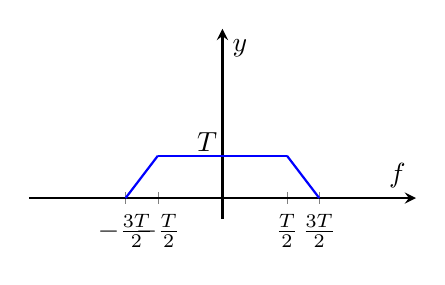
\begin{tikzpicture}
                    \begin{axis}[
                        xlabel=$f$,
                        ylabel=$y$,
                        xmin=-3,
                        xmax=3,
                        ymin=-0.5,
                        ymax=4,
                        ytick = {1},
                        xtick={-3/2,-1, 0,1, 3/2},
                        xticklabels={$-\frac{3T}{2}$,$-\frac{T}{2}$, $0$,$\frac{T}{2}$ ,$\frac{3T}{2}$},
                        yticklabels = {$T$},
                        yticklabel style = {yshift=5pt,xshift=4pt}, 
                        axis lines=middle,
                        thick,
                        domain=-3:3,
                        samples=100,
                        width=6.5cm,
                        height=4cm
                    ]
                        
                    \addplot [sharp plot, blue, thick] coordinates{(-3/2,0)(-1,1)};
                    \addplot [sharp plot, blue, thick] coordinates{(3/2,0)(1,1)};
                    \addplot [sharp plot, blue, thick] coordinates{(-1,1)(1,1)};
                
                    \end{axis}
                \end{tikzpicture}
                \label{fig:PC rect in rect diverse}
            }
            \caption{Integrale di convoluzione di $rect$ di durata diversa}
        \end{figure}
        Esemptio $TCF$ di un triangolo:
        \begin{figure}[H]
            \centering
            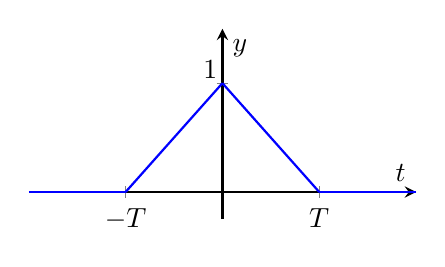
\begin{tikzpicture}
                \begin{axis}[
                    xlabel=$t$,
                    ylabel=$y$,
                    xmin=-4,
                    xmax=4,
                    ymin=-0.5,
                    ymax=3,
                    ytick = {2},
                    xtick={-2, 0, 2},
                    xticklabels={$-T$, $0$, $T$},
                    yticklabels = {$1$},
                    yticklabel style = {yshift=5pt,xshift=4pt}, 
                    axis lines=middle,
                    thick,
                    domain=-4:4,
                    samples=100,
                    width=6.5cm,
                    height=4cm
                ]
                \addplot [sharp plot, blue, thick] coordinates{(-2,0)(0,2)};
                \addplot [sharp plot, blue, thick] coordinates{(2,0)(0,2)};
            
                \addplot [const plot, blue, thick] coordinates{(-2,0)(-4,0)};
                \addplot [const plot, blue, thick] coordinates{(2,0)(4,0)};
            
                \end{axis}
            \end{tikzpicture}
            \label{fig:PC TCF triangolo}
            \caption{Integrale di convoluzione}
        \end{figure}
        Dal Th. di Convoluzione \ref{Convoluzione} sappiamo che é il prodotto di convoluzione di 2 rect di durata uguale a $T$:
        \begin{gather}
            z_{(t)} = x_{(t)}\otimes y_{(t)} = rect\left(\frac{t}{T}\right) \otimes rect\left(\frac{t}{T}\right) \overset{Th. \ref{Convoluzione}}{\Rightarrow} Tsinc(fT)\dotproduct Tsinc(fT) \nonumber \\
            T^2sinc^2(fT) \nonumber 
        \end{gather}
        % Esercizio appunti martorella triangoli a sx a dx:
    \subsection{Modulazione di Ampiezza}\label{Modulazione di Ampiezza}
        % \[
        %     y_{(t)} = x_{(t)}\cos(2\pi f_0t)
        % \]
        \begin{figure}[H]
            \centering
            \subfloat[Sistema di modulazione]{
                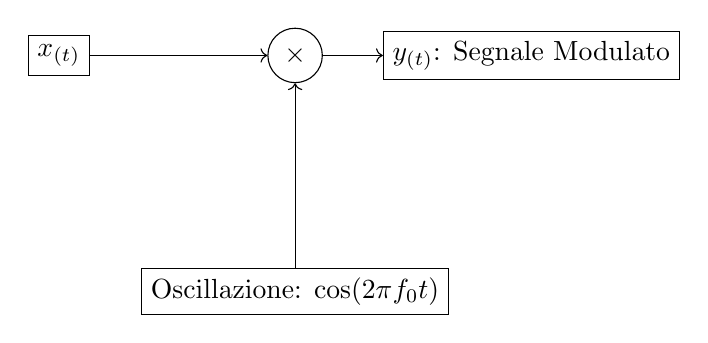
\begin{tikzpicture}[
                        node distance=3cm
                    ]
                    % Blocks
                    \node [rectangle, draw] (input) {$x_{(t)}$};
                    \node [circle, draw, right of=input] (product) {$\times$};
                    \node [rectangle, draw, below of=product] (carrier) {Oscillazione: $\cos(2\pi f_0t)$};
                    \node [rectangle, draw, right of=product] (modulated) {$y_{(t)}$: Segnale Modulato};
                
                    % Connections
                    \draw [->] (input) -- (product);
                    \draw [->] (product) -- (modulated);
                    \draw [->] (carrier) -- (product);
                \end{tikzpicture}    
                \label{fig:sistema di modulazione}
            }
            \hfill
            \subfloat[{\color{blue}$x_{(t)}$}, {\color{red}$y_{(t)}$}, {\color{purple}$\cos (2\pi t)$}]{
                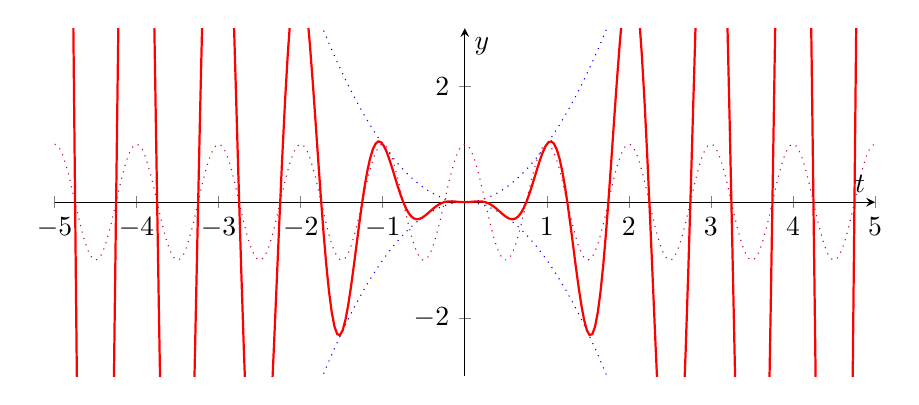
\begin{tikzpicture}
                    \begin{axis}[
                        domain=-5:5,
                        samples=200,
                        axis lines=middle,
                        xlabel=$t$,
                        ylabel=$y$,
                        ymin=-3,
                        ymax=3,
                        width=12cm,
                        height=6cm
                    ]
                    \addplot [blue, dotted, samples = 300] {(x^2)};
                    \addplot [blue, dotted, samples = 300] {-(x^2)};
                    \addplot [purple,dotted, samples = 300] {cos(deg(2*pi*x))};
                    \addplot [red, thick, samples = 300] {cos(deg(2*pi*x))*(x^2)};
                    \end{axis}
                \end{tikzpicture}
                \label{fig:modulazione in ampiezza}
            }
            \caption{Esempio sistema di modulazione di ampiezza}
        \end{figure}
        L'oscillazione introdotta, $\cos (2\pi t)$, segue l'andamento di $x_{(t)}$
        Nel dominio della frequenza:
        \begin{figure}[H]
            \centering
            \subfloat[Senza modulazione]{
                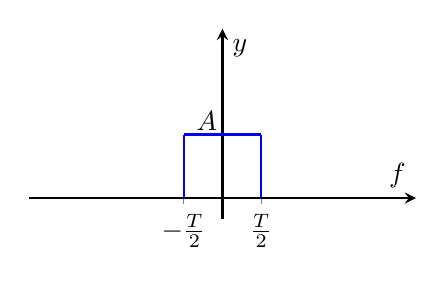
\begin{tikzpicture}
                    \begin{axis}[
                        xlabel=$f$,
                        ylabel=$y$,
                        xmin=-5,
                        xmax=5,
                        ymin=-0.5,
                        ymax=4,
                        ytick = {1.5},
                        xtick={-1, 0, 1},
                        xticklabels={$-\frac{T}{2}$, $0$, $\frac{T}{2}$},
                        yticklabels = {$A$},
                        yticklabel style = {yshift=5pt,xshift=4pt}, 
                        axis lines=middle,
                        thick,
                        domain=-5:5,
                        samples=100,
                        width=6.5cm,
                        height=4cm
                    ]
                    \addplot [const plot, blue, thick] coordinates{(-1,1.5)(1,1.5)};
                    \addplot [const plot, blue, thick] coordinates{(-1,0)(-1,1.5)};
                    \addplot [const plot, blue, thick] coordinates{(1,0)(1,1.5)};
                
                    \end{axis}
                \end{tikzpicture}
                \label{fig:segnale senza modulazione}
            }
            \hfill
            \subfloat[Con modulazione]{
                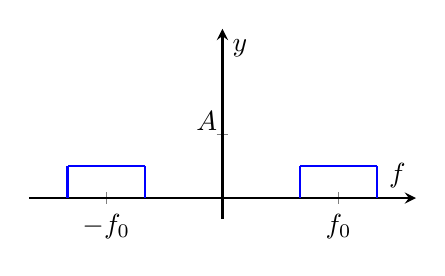
\begin{tikzpicture}
                    \begin{axis}[
                        xlabel=$f$,
                        ylabel=$y$,
                        xmin=-5,
                        xmax=5,
                        ymin=-0.5,
                        ymax=4,
                        ytick = {1.5},
                        xtick={-3,0,3},
                        xticklabels={$-f_0$, $0$,$f_0$},
                        yticklabels = {$A$},
                        yticklabel style = {yshift=5pt,xshift=4pt}, 
                        axis lines=middle,
                        thick,
                        domain=-5:5,
                        samples=100,
                        width=6.5cm,
                        height=4cm
                    ]
                    \addplot [const plot, blue, thick] coordinates{(-2,0.75)(-4,0.75)};
                    \addplot [const plot, blue, thick] coordinates{(-2,0)(-2,0.75)};
                    \addplot [const plot, blue, thick] coordinates{(-4,0)(-4,0.75)};
                    
                    \addplot [const plot, blue, thick] coordinates{(2,0.75)(4,0.75)};
                    \addplot [const plot, blue, thick] coordinates{(2,0)(2,0.75)};
                    \addplot [const plot, blue, thick] coordinates{(4,0)(4,0.75)};
                    
                    \end{axis}
                \end{tikzpicture}
                \label{fig:segnale con modulazione}
            }
            \caption{Segnale nel dominio della frequenza modulato e non}
        \end{figure}
        Serve per spostare la frequenza (es. di trasmissione) del segnale in modo tale, ad esempio, da non sovrapporre due segnali che sono sulla stessa frequenza.
        Se il segnale non fosse modulato si dice in {\color{blue} \textbf{banda base} (BB)} se il segnale é modulato si dice in {\color{red}\textbf{banda passante}(BP)}.
        \begin{figure}[H]
            \centering
            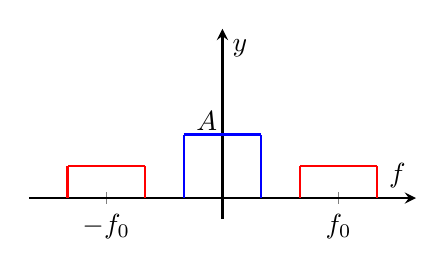
\begin{tikzpicture}
                \begin{axis}[
                    xlabel=$f$,
                    ylabel=$y$,
                    xmin=-5,
                    xmax=5,
                    ymin=-0.5,
                    ymax=4,
                    ytick = {1.5},
                    xtick={-3,0,3},
                    xticklabels={$-f_0$, $0$,$f_0$},
                    yticklabels = {$A$},
                    yticklabel style = {yshift=5pt,xshift=4pt}, 
                    axis lines=middle,
                    thick,
                    domain=-5:5,
                    samples=100,
                    width=6.5cm,
                    height=4cm
                ]
                \addplot [const plot, red, thick] coordinates{(-2,0.75)(-4,0.75)};
                \addplot [const plot, red, thick] coordinates{(-2,0)(-2,0.75)};
                \addplot [const plot, red, thick] coordinates{(-4,0)(-4,0.75)};
                
                \addplot [const plot, red, thick] coordinates{(2,0.75)(4,0.75)};
                \addplot [const plot, red, thick] coordinates{(2,0)(2,0.75)};
                \addplot [const plot, red, thick] coordinates{(4,0)(4,0.75)};
            
                \addplot [const plot, blue, thick] coordinates{(-1,1.5)(1,1.5)};
                \addplot [const plot, blue, thick] coordinates{(-1,0)(-1,1.5)};
                \addplot [const plot, blue, thick] coordinates{(1,0)(1,1.5)};
            
                
                \end{axis}
            \end{tikzpicture}
            \caption{{\color{blue}BB}, {\color{red}BP}}
            \label{fig:bb e bp}
        \end{figure}

        \subsubsection{Th. Modulazione con $\cos(2\pi f_0t)$}\label{Modulazione con coseno}
            $Ip:\begin{cases}
                    y_{(t)}= x_{(t)}\cos(2\pi f_0t)\\        
                    x_{(t)}\overunderset{TCF}{ATCF}{\leftrightharpoons} X_{(f)}
                \end{cases}$\\
            $Th: Y_{(f)} = \frac{1}{2} X_{(f-f_0)} + \frac{1}{2} X_{(f+f_0)}$ \\
            Dimostrazione:
            \begin{align}
                Y_{(f)} & = \int_{-\infty}^{\infty} y_{(t)} e^{-j2\pi ft} dt = \int_{-\infty}^{\infty} x_{(t)}\cos(2\pi f_0t) e^{-j2\pi ft} dt \nonumber \\
                & =\int_{-\infty}^{\infty} x_{(t)} \frac{e^{j2\pi f_0t} + e^{-j2\pi f_0t}}{2} e^{-j2\pi ft} dt =  \nonumber \\
                & = \frac{1}{2} \int_{-\infty}^{\infty} x_{(t)} e^{-j2\pi (f-f_0)t} dt + \frac{1}{2} \int_{-\infty}^{\infty} x_{(t)} e^{-j2\pi (f+f_0)t} dt \nonumber \\
                & = \eval{TCF[x_{(t)}]}_{f-f_0} + \eval{TCF[x_{(t)}]}_{f+f_0} = \frac{1}{2} X_{(f-f_0)} + \frac{1}{2} X_{(f+f_0)}\ c.v.d \nonumber  
            \end{align}
            Esempio:\\
            {
                $X_{(f)} = \frac{A}{B}rect\left(\frac{f}{B}\right)$
                \[
                    Y_{(f)} = \frac{A}{2B}rect\left(\frac{f-f_0}{B}\right)+\frac{A}{2B}rect\left(\frac{f+f_0}{B}\right)
                \]
                \begin{figure}[H]
                    \centering
                    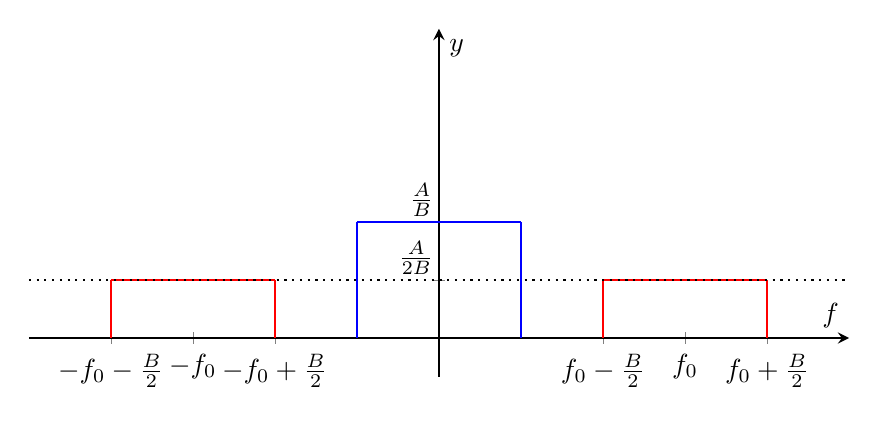
\begin{tikzpicture}
                        \begin{axis}[
                            xlabel=$f$,
                            ylabel=$y$,
                            xmin=-5,
                            xmax=5,
                            ymin=-0.5,
                            ymax=4,
                            ytick = {0.75,1.5},
                            xtick={-4,-3,-2, 0,2,3,4},
                            xticklabels={$-f_0-\frac{B}{2}$,$-f_0$,$-f_0+\frac{B}{2}$,$0$,$f_0-\frac{B}{2}$,$f_0$,$f_0+\frac{B}{2}$},
                            yticklabels = {$\frac{A}{2B}$,$\frac{A}{B}$},
                            yticklabel style = {yshift=8pt,xshift=4pt}, 
                            axis lines=middle,
                            thick,
                            domain=-5:5,
                            samples=100,
                            width=12cm,
                            height=6cm
                        ]
                        \addplot [const plot, red, thick] coordinates{(-2,0.75)(-4,0.75)};
                        \addplot [const plot, red, thick] coordinates{(-2,0)(-2,0.75)};
                        \addplot [const plot, red, thick] coordinates{(-4,0)(-4,0.75)};
                        
                        \addplot [const plot, red, thick] coordinates{(2,0.75)(4,0.75)};
                        \addplot [const plot, red, thick] coordinates{(2,0)(2,0.75)};
                        \addplot [const plot, red, thick] coordinates{(4,0)(4,0.75)};
                    
                        \addplot [const plot, blue] coordinates{(-1,1.5)(1,1.5)};
                        \addplot [const plot, blue] coordinates{(-1,0)(-1,1.5)};
                        \addplot [const plot, blue] coordinates{(1,0)(1,1.5)};
                        
                        \addplot [const plot,dotted, black] coordinates{(-5,0.75)(5,0.75)};

                        \end{axis}
                    \end{tikzpicture}
                    \caption{{\color{blue}$X_{(f)}$}, {\color{red}$Y_{(f)}$}}
                    \label{fig:modulazione rect}
                \end{figure}
            }
        \subsubsection{Th. Modulazione con $\sin(2\pi f_0t)$}\label{Modulazione con seno}
        $Ip:\begin{cases}
                y_{(t)}= x_{(t)}\sin(2\pi f_0t)\\        
                x_{(t)}\overunderset{TCF}{ATCF}{\leftrightharpoons} X_{(f)}
            \end{cases}$\\
        $Th: Y_{(f)} = \frac{1}{2j} X_{(f-f_0)} - \frac{1}{2j} X_{(f+f_0)} $ \\
        Dimostrazione: 
        \begin{align}
            Y_{(f)} & = \int_{-\infty}^{\infty} y_{(t)} e^{-j2\pi ft} dt = \int_{-\infty}^{\infty} x_{(t)}\sin(2\pi f_0t) e^{-j2\pi ft} dt \nonumber \\
            & =\int_{-\infty}^{\infty} x_{(t)} \frac{e^{j2\pi f_0t} - e^{-j2\pi f_0t}}{2j} e^{-j2\pi ft} dt =  \nonumber \\
            & = \frac{1}{2j} \int_{-\infty}^{\infty} x_{(t)} e^{-j2\pi (f-f_0)t} dt - \frac{1}{2j} \int_{-\infty}^{\infty} x_{(t)} e^{-j2\pi (f+f_0)t} dt \nonumber \\
            & = \eval{TCF[x_{(t)}]}_{f-f_0} - \eval{TCF[x_{(t)}]}_{f+f_0} = \frac{1}{2j} X_{(f-f_0)} - \frac{1}{2j} X_{(f+f_0)}\ c.v.d \nonumber  
        \end{align}

        \subsubsection{Th. Modulazione con $\cos(2\pi f_0t + \phi)$}\label{Modulazione con coseno generico}
            $Ip: \begin{cases}
                y_{(t)}= x_{(t)}\cos(2\pi f_0t + \phi)\\        
                x_{(t)}\overunderset{TCF}{ATCF}{\leftrightharpoons} X_{(f)}
                \end{cases}$\\
            $Th: Y_{(f)} = \frac{e^{j\phi}}{2} X_{(f-f_0)} + \frac{e^{-j\phi}}{2} X_{(f+f_0)} $ \\
            Dimostrazione: 
            \begin{align}
                Y_{(f)} & = \int_{-\infty}^{\infty} y_{(t)} e^{-j2\pi ft} dt = \int_{-\infty}^{\infty} x_{(t)}\cos(2\pi f_0t + \phi) e^{-j2\pi ft} dt \nonumber \\
                & =\int_{-\infty}^{\infty} x_{(t)} \frac{e^{j(2\pi f_0t+ \phi)} + e^{-j(2\pi f_0t+ \phi)}}{2} e^{-j2\pi ft} dt =  \nonumber \\
                & = \frac{e^{j\phi}}{2} \int_{-\infty}^{\infty} x_{(t)} e^{-j2\pi (f-f_0)t} dt + \frac{e^{-j\phi}}{2} \int_{-\infty}^{\infty} x_{(t)} e^{-j2\pi (f+f_0)t} dt \nonumber \\
                & = \eval{TCF[x_{(t)}]}_{f-f_0} + \eval{TCF[x_{(t)}]}_{f+f_0} = \frac{e^{j\phi}}{2} X_{(f-f_0)} + \frac{e^{-j\phi}}{2} X_{(f+f_0)}\ c.v.d \nonumber  
            \end{align}
            Esempio:
            \begin{figure}[H]
                \centering
                \subfloat[Ampiezza Mod. generica]{
                    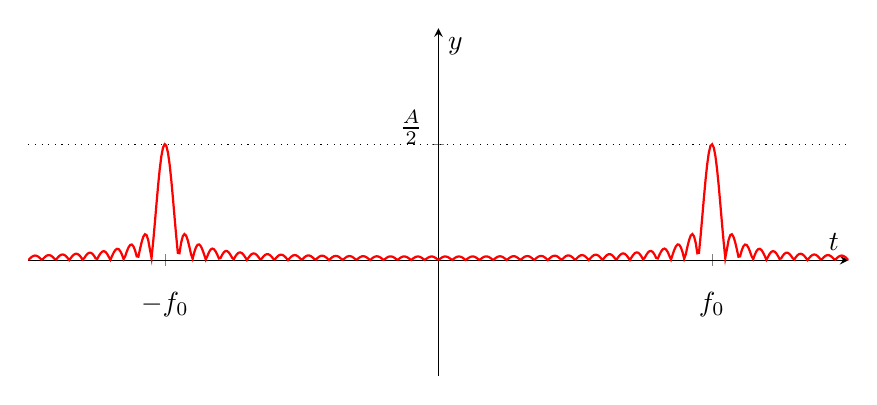
\begin{tikzpicture}
                        \begin{axis}[
                            domain=-30:30,
                            samples=200,
                            axis lines=middle,
                            xlabel=$t$,
                            ylabel=$y$,
                            ytick = {0.5},
                            yticklabels = {$\frac{A}{2}$},
                            yticklabel style = {yshift=6pt},
                            xtick = {-20,20},
                            xticklabels = {$-f_0$,$f_0$},
                            xticklabel style = {yshift=-6pt}, 
                            ymin=-0.5,
                            ymax=1,
                            width=12cm,
                            height=6cm
                        ]
                        \addplot [const plot, dotted,black] coordinates{(-30,0.5)(30,0.5)};
                        \addplot [red, thick, samples = 500] {abs(sin(deg((x-20)*pi))/(2*(x-20)*pi))+abs(sin(deg((x+20)*pi))/(2*(x+20)*pi))};
                        % \addplot [red, thick, samples = 500] {abs(sin(deg((x+20)*pi))/(2*(x+20)*pi))};
                        \end{axis}
                    \end{tikzpicture}
                    \label{fig:Ampiezza Mod. generica}
                }
                \hfill
                \subfloat[fase Mod. generica]{
                        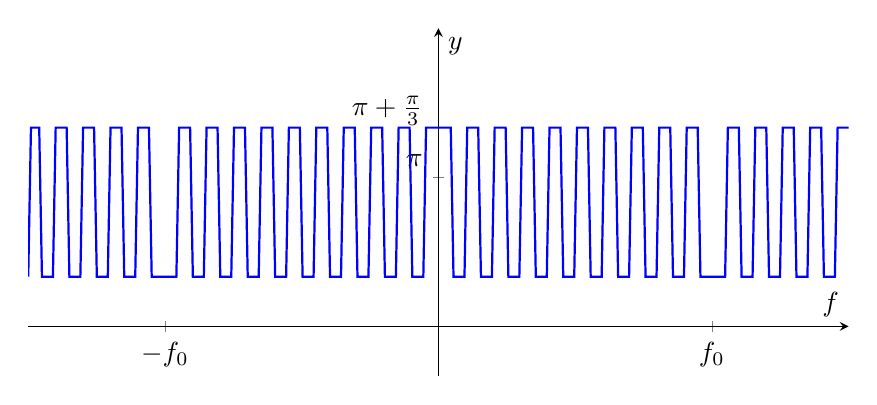
\begin{tikzpicture}
                            \begin{axis}[
                                domain=-30:30,
                                samples=200,
                                axis lines=middle,
                                xlabel=$f$,
                                ylabel=$y$,
                                ymin=-pi/3,
                                ymax=2*pi,
                                xtick={-20,20},
                                xticklabels={$-f_0$,$f_0$},
                                ytick={pi,pi+(pi*1/3)},
                                yticklabel style = {yshift=6pt}, 
                                yticklabels={$\pi$,$\pi+\frac{\pi}{3} $},
                                width=12cm,
                                height=6cm
                            ]
                            \addplot [blue, thick, samples = 300] {rad(atan2(0,(x*sin(deg(pi*x)))/(pi*(-400 + x^2))))+(pi*1/3)};
                            \end{axis}
                        \end{tikzpicture}
                    \label{fig:fase Mod. generica}
                }
                \caption{Modulazione generica di una $A rect\left(\frac{t}{T}\right)$ con $\cos(2\pi f_0t+\frac{\pi}{3})$}
            \end{figure}
        % É legale cosa ho scritto sopra della modulazione generica?
        \subsubsection{Th. Modulazione con Esponenziale Complesso}\label{Modulazione con Esponenziale Complesso}
            $Ip: \begin{cases}
                y_{(t)}= x_{(t)}e^{j2\pi f_0t}\\        
                x_{(t)}\overunderset{TCF}{ATCF}{\leftrightharpoons} X_{(f)}
                \end{cases}$\\
            $Th: Y_{(f)} = X_{(f-f_0)} $ \\
            Dimostrazione: 
            \begin{align}
                Y_{(f)} & = \int_{-\infty}^{\infty} y_{(t)} e^{-j2\pi ft} dt = \int_{-\infty}^{\infty} x_{(t)}e^{j2\pi f_0t} e^{-j2\pi ft} dt \nonumber \\
                & =\int_{-\infty}^{\infty} x_{(t)} e^{-j2\pi (f-f_0)t} dt = \eval{TCF[x_{(t)}]}_{f-f_0} = X_{(f-f_0)} \nonumber
            \end{align}
            Posso notare che:
            \begin{itemize}
                \item Ritardo: $\rightarrow x_{(t-t_0)} \rightleftharpoons X_{(f)} e^{(-j2\pi ft_0)}$
                \item Modulazione: $\rightarrow x_{(t)}e^{(j2\pi f_0t)} \rightleftharpoons X_{(f-f_0)}$
            \end{itemize}
            Procedimento per la sintesi di un segnale:
            \begin{itemize}
                \item Derivo il segnale
                \item Verifico le ipotesi del Th. dell'Integrazione \ref{Integrazione}
                \item calcolo la TCF della derivata
                \item Applico il Th. dell'integrazione per calcolare $X_{(f)}$
            \end{itemize}

            \subsubsection{Demodulazione}\label{Demodulazione}
            Ci poniamo il problema di riportare il segnale modulato al segnale originale($g_{(t)}$), dato:\\
            $x_{(t)} = g_{(t)} \cos(2\pi f_0t)$\\
            Demoduliamo il segnale con $2\cos(2\pi f_0t)$:
            \begin{align}
                y_{(t)} &= x_{(t)} {\color{purple}2}\cos(2\pi f_0t) = g_{(t)} \cos^2(2\pi f_0t) \nonumber \\
                        &= g_{(t)} \frac{1+ \cos(4\pi f_0t)}{2} = \frac{g_{(t)}}{2} + \frac{g_{(t)}\cos(4\pi f_0t)}{2}\nonumber\\
                TCF[y_{(t)}] &\overset{Th. \ref{Modulazione con coseno}}{\Rightarrow}  \frac{2G_{(f)}}{2} + \frac{2G_{(f-2f_0)}}{2}+ \frac{2G_{(f+2f_0)}}{2} \nonumber \\
                        &= G_{(f)}+G_{(f-2f_0)}+G_{(f+2f_0)}
            \end{align}
            Dall'ultima uguagliaza posso quindi usare un filtro in ({\color{blue}BB}) per rimuovere i segnali alle frequenze $\pm 2f_0$ e ricavare il mio segnale $G_{(f)}$.\\
            Riporto un po di esempi di demodulazione di una o piú $rect$:
            Esempio di Demodulazione
            \begin{figure}[H]
                \centering
                \subfloat[$sinc$ modulata]{
                    \begin{tikzpicture}
                        \begin{axis}[
                            domain=-40:40,
                            samples=200,
                            axis lines=middle,
                            xlabel=$t$,
                            ylabel=$y$,
                            ytick = {0.5},
                            yticklabels = {$\frac{A}{2}$},
                            yticklabel style = {yshift=6pt},
                            xtick = {-10,10},
                            xticklabels = {$-f_0$,$f_0$},
                            xticklabel style = {yshift=-6pt}, 
                            ymin=-0.5,
                            ymax=1,
                            width=12cm,
                            height=6cm
                        ]
                        \addplot [const plot, dotted,black] coordinates{(-30,0.5)(30,0.5)};
                        \addplot [red, thick, samples = 500] {(sin(deg((x-10)*pi))/(2*(x-10)*pi))+(sin(deg((x+10)*pi))/(2*(x+10)*pi))};
                        \end{axis}
                    \end{tikzpicture}
                    \label{fig:sinc modulata}
                }
                \hfill
                \subfloat[$sinc$ demodulata]{
                    \begin{tikzpicture}
                        \begin{axis}[
                            domain=-40:40,
                            samples=200,
                            axis lines=middle,
                            xlabel=$t$,
                            ylabel=$y$,
                            ytick = {0.5},
                            yticklabels = {$\frac{A}{2}$},
                            yticklabel style = {yshift=6pt,xshift=-6pt},
                            xtick = {-20,20},
                            xticklabels = {$-2f_0$,$2f_0$},
                            xticklabel style = {yshift=-6pt}, 
                            ymin=-0.5,
                            ymax=1,
                            width=12cm,
                            height=6cm
                        ]
                        \addplot [const plot, dotted,black] coordinates{(-30,0.5)(30,0.5)};
                        \addplot [const plot,blue] coordinates{(-2,-0.5)(-2,1)};
                        \addplot [const plot,blue] coordinates{(2,-0.5)(2,1)};
                        \addplot [red, thick, samples = 500] {(sin(deg((x)*pi))/(2*(x)*pi))+(sin(deg((x-20)*pi))/(2*(x-20)*pi))+(sin(deg((x+20)*pi))/(2*(x+20)*pi))};
                        \end{axis}
                    \end{tikzpicture}
                    \label{fig:demodulazione di una sinc}
                }
                \caption{Demodulazione di una $sinc$}
            \end{figure}
            Nel caso di piú segnali durante la demodulazione il segnale che voglio recuperare viene spostato in {\color{blue}BB}
            mentre gli altri segnali presenti sullo spettro vengono a loro volta modulati peró con un $f_0$ diverso rispetto al loro $f_0^\prime$:
            \begin{figure}[H]
                \centering
                \subfloat[Due $sinc$ modulate]{
                    \begin{tikzpicture}
                        \begin{axis}[
                            domain=-55:55,
                            samples=200,
                            axis lines=middle,
                            xlabel=$t$,
                            ylabel=$y$,
                            ytick = {0.5},
                            yticklabels = {$\frac{A}{2}$},
                            yticklabel style = {yshift=6pt},
                            xtick = {-40,-10,10,40},
                            xticklabels = {$-f_0^\prime$,$-f_0$,$f_0$,$f_0^\prime$},
                            xticklabel style = {yshift=-7pt}, 
                            ymin=-0.5,
                            ymax=1,
                            width=14cm,
                            height=6cm
                        ]
                        \addplot [const plot, dotted,black] coordinates{(-30,0.5)(30,0.5)};
                        \addplot [red, thick, samples = 500] {(sin(deg((x-10)*pi))/(2*(x-10)*pi))+(sin(deg((x+10)*pi))/(2*(x+10)*pi))+(sin(deg((x-40)*pi))/((x-40)*pi))+(sin(deg((x+40)*pi))/((x+40)*pi))};
                        \end{axis}
                    \end{tikzpicture}
                    \label{fig:due sinc modulate}
                }
                \hfill
                \subfloat[Demodulazione delle $sinc$]{
                    \begin{tikzpicture}
                        \begin{axis}[
                            domain=-55:55,
                            samples=200,
                            axis lines=middle,
                            xlabel=$t$,
                            ylabel=$y$,
                            ytick = {0.5},
                            yticklabels = {$\frac{A}{2}$},
                            yticklabel style = {yshift=6pt,xshift=-6pt},
                            xtick = {-50,-40,-30,-20,20,30,40,50},
                            xticklabels = {$-f_0^\prime-f_0$,$-f_0^\prime$,$-f_0^\prime+f_0$,$-2f_0$,$2f_0$,$f_0^\prime-f_0$,$f_0^\prime$,$f_0^\prime+f_0$},
                            xticklabel style = {yshift=-6pt,font=\tiny}, 
                            ymin=-0.5,
                            ymax=1,
                            width=14cm,
                            height=6cm
                        ]
                        \addplot [const plot, dotted,black] coordinates{(-30,0.5)(30,0.5)};
                        \addplot [const plot,blue] coordinates{(-2,-0.5)(-2,1)};
                        \addplot [const plot,blue] coordinates{(2,-0.5)(2,1)};
                        \addplot [red, thick, samples = 800] {(sin(deg((x)*pi))/(2*(x)*pi))+(sin(deg((x-20)*pi))/(2*(x-20)*pi))+(sin(deg((x+20)*pi))/(2*(x+20)*pi))+(sin(deg((x-50)*pi))/(2*(x-50)*pi))+(sin(deg((x-30)*pi))/(2*(x-30)*pi))+(sin(deg((x+50)*pi))/(2*(x+50)*pi))+(sin(deg((x+30)*pi))/(2*(x+30)*pi))};
                        \end{axis}
                    \end{tikzpicture}
                    \label{fig:demodulazione di due sinc}
                }
                \caption{Demodulazione di due $sinc$}
            \end{figure}
            Potrei peró trovarmi in situazioni delle quali non posso recuperare il segnale
            \begin{figure}[H]
                \centering
                \subfloat[Due $sinc$ modulate]{
                    \begin{tikzpicture}
                        \begin{axis}[
                            domain=-55:55,
                            samples=200,
                            axis lines=middle,
                            xlabel=$t$,
                            ylabel=$y$,
                            ytick = {0.5},
                            yticklabels = {$\frac{A}{2}$},
                            yticklabel style = {yshift=6pt},
                            xtick = {-20,-18,18,20},
                            xticklabels = {$-f_0^\prime$,$-f_0$,$f_0$,$f_0^\prime$},
                            xticklabel style = {yshift=-7pt,font=\tiny}, 
                            ymin=-0.5,
                            ymax=1,
                            width=14cm,
                            height=6cm
                        ]
                        \addplot [const plot, dotted,black] coordinates{(-30,0.5)(30,0.5)};
                        \addplot [red, thick, samples = 500] {(sin(deg((x-18)*pi))/(2*(x-18)*pi))+(sin(deg((x+18)*pi))/(2*(x+18)*pi))+(sin(deg((x-20)*pi))/((x-20)*pi))+(sin(deg((x+20)*pi))/((x+20)*pi))};
                        \end{axis}
                    \end{tikzpicture}
                    \label{fig:sinc non recuperabile}
                }
                \hfill
                \subfloat[Demodulazione delle $sinc$]{
                    \begin{tikzpicture}
                        \begin{axis}[
                            domain=-55:55,
                            samples=200,
                            axis lines=middle,
                            xlabel=$t$,
                            ylabel=$y$,
                            ytick = {0.5},
                            yticklabels = {$\frac{A}{2}$},
                            yticklabel style = {yshift=6pt,xshift=-6pt},
                            xtick = {-38,-36,-2,2,36,38},
                            xticklabels = {$-f_0^\prime-f_0$,,$-2f_0$$-f_0^\prime+f_0$,$f_0^\prime-f_0$,$2f_0$,$f_0^\prime+f_0$},
                            xticklabel style = {yshift=-6pt,font=\tiny,rotate=90}, 
                            ymin=-0.5,
                            ymax=1,
                            width=14cm,
                            height=6cm
                        ]
                        \addplot [const plot, dotted,black] coordinates{(-30,0.5)(30,0.5)};
                        \addplot [const plot,blue] coordinates{(-2,-0.5)(-2,1)};
                        \addplot [const plot,blue] coordinates{(2,-0.5)(2,1)};
                        \addplot [red, thick, samples = 800] {(sin(deg((x)*pi))/(2*(x)*pi))+(sin(deg((x-36)*pi))/(2*(x-36)*pi))+(sin(deg((x+36)*pi))/(2*(x+36)*pi))+(sin(deg((x-38)*pi))/(2*(x-38)*pi))+(sin(deg((x-2)*pi))/(2*(x-2)*pi))+(sin(deg((x+38)*pi))/(2*(x+38)*pi))+(sin(deg((x+2)*pi))/(2*(x+2)*pi))};
                        \end{axis}
                    \end{tikzpicture}
                    \label{fig:demodulazione sinc non recuperabile}
                }
                \caption{Demodulazione di due $sinc$ non recuperabili}
            \end{figure}
            Come possiamo vedere nella regione della {\color{blue}BB}, il segnale é molto sporco, magari puó essere confuso con un 
            $\cos$ e non una sinc. inoltre ora qui ho usato numeri interi per fare il $plot$ quindi non si accavallano cosí male 
            ma si accavallano solo in $\frac{1}{T}$ se usassi altri valori sarebbe ancora piú sporco il segnale.\\
            
            Adesso proviamo a calcolare quanti segnali possiamo trasmettere in una banda:\\
            
            \indent{
                Ho un segnale rettangolare che dura $5$ minuti e una banda di $20MHz = 20\dotproduct 10^6Hz$\\
                \begin{gather}
                        f_{segnale}=\frac{1}{5\dotproduct60} =\frac{1}{300}Hz  \nonumber \\
                        n^{\circ}\ di\ segnali = \frac{20\dotproduct 10^6}{f_{segnale}} = 20\dotproduct 10^6 \dotproduct 300 = 6\dotproduct 10^9 \nonumber
                \end{gather}
            }
            \begin{figure}[H]
                \centering
                \begin{tikzpicture}
                    \begin{axis}[
                        domain=-4:4,
                        samples=200,
                        axis lines=middle,
                        xlabel=$x$,
                        ymin=-0.2,
                        ymax=0.2,
                        xtick={-2,0,2},
                        xticklabels={$f_{lower\ bound}$,$0$,$f_{upper\ bound}$},
                        ytick={},
                        width=10cm,
                        height=4cm
                    ]
                    \addplot [const plot,blue, thick] coordinates{(-2,0)(2,0)};
                    \end{axis}
                \end{tikzpicture}
                \caption{Spettro per la trasmissione}
                \label{fig:banda esercizio segnali}
            \end{figure}    
            \subsubsection{Radar}
                \begin{figure}[H]
                    \centering
                    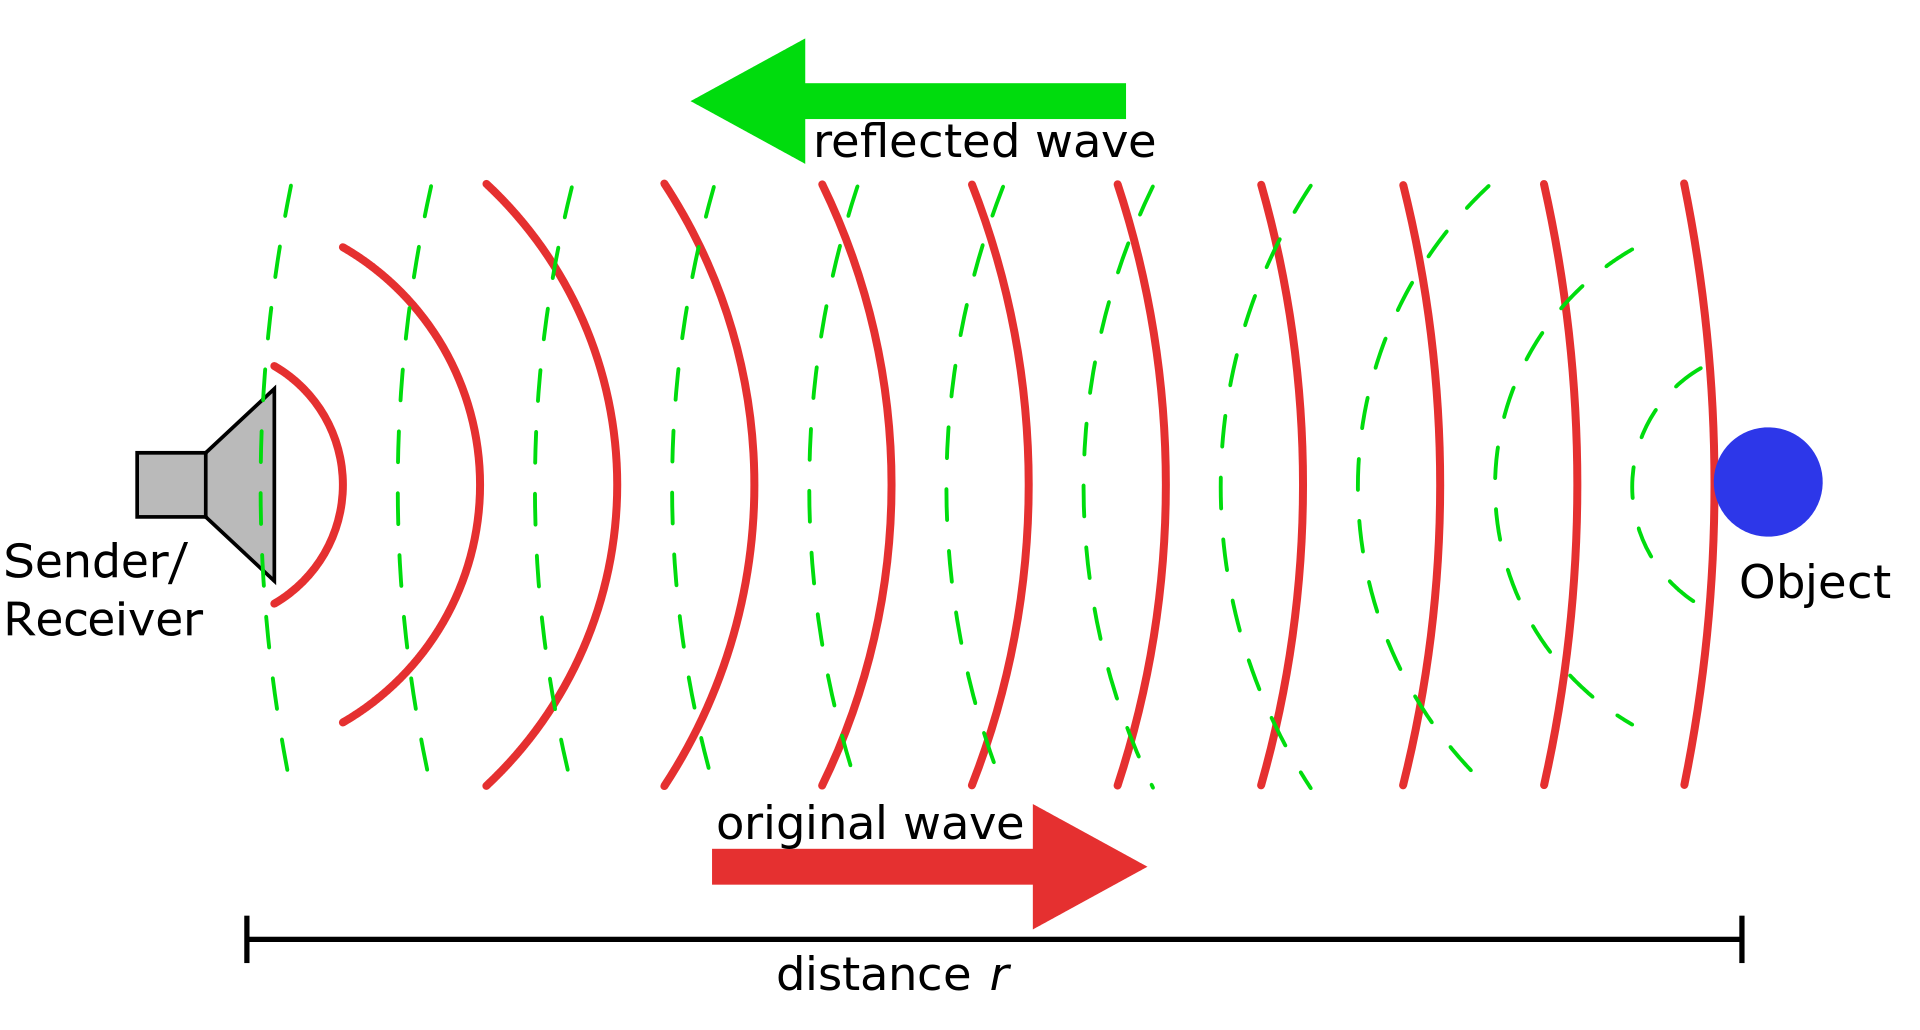
\includegraphics[width=8cm]{media/radar.png}
                    \caption{Spettro per la trasmissione}
                    \label{fig:esempio radar}
                \end{figure}    
                La sorgente emette un'{\color{red}onda} continua e passivamente capta per le {\color{green}onde} riflesse dagli oggetti.
                Il calcolo della distanza si basa sulla capacitá dei materiali di riflettere le onde, piú la frequenza dell'onda é alta 
                piú i materiali riescono a riflettere. L'emettitore, in presenza di ostacolo, riceve il segnale riflesso ({\em eco})
                e misura il ritardo dell'{\em eco} rispetto al segnale originale per poi calcolarne la distanza. Prendiamo un emettitore di onde 
                rettangolari.
                \begin{figure}[H]
                    \centering
                    \begin{tikzpicture}
                        \begin{axis}[
                            domain=-0:10,
                            samples=200,
                            axis lines=middle,
                            xlabel=$t$,
                            ylabel=$y$,
                            ymin=-0.2,
                            ymax=3,
                            xtick={0,2,4,6},
                            xticklabels={$0$,$T$,$\tau$,$\tau+T$},
                            ytick={},
                            width=10cm,
                            height=4cm
                        ]
                        \addplot [const plot,red, thick] coordinates{(0,0)(0,2)};
                        \addplot [const plot,red, thick] coordinates{(0,2)(2,2)};
                        \addplot [const plot,red, thick] coordinates{(2,2)(2,0)};

                        \addplot [const plot,green, thick] coordinates{(4,0)(4,1)};
                        \addplot [const plot,green, thick] coordinates{(4,1)(6,1)};
                        \addplot [const plot,green, thick] coordinates{(6,1)(6,0)};
                        \end{axis}
                    \end{tikzpicture}
                    \caption{Spettro per la trasmissione}
                    \label{fig:radar rettangolare}
                \end{figure}    
                Indichiamo con $\tau$ il ritardo di ricezione dell'{\em eco} e la distanza che sempara il radar dall'oggetto $d$:
                \[
                    d=\frac{c\tau}{2}
                \]
                Compare un fattore $\frac{1}{2}$ dovuto al segnale che percorre due volte la distanza tra l'emettitore e l'oggetto.
                Possiamo notare che l'{\em eco} ha ampiezza minore poiché dell'energia é stata assorbita dal materiale o una porzione del segnale
                originale ha oltrepassato il materiale stesso.
                
                Analizziamo in frequenza cosa succede. 
                
                Volgiamo realizzare un radar a onda rettagolare che rileva a un massimo di $15$ metri di distanza e a un minimo di $1,5$ metri.
                Possiamo calcolare i valori di ritardo massimo e minimo:
                \begin{gather}
                    \tau_{min} =\frac{2\dotproduct 15}{3\dotproduct 10^8} =10^{-7} = 0.1\mu s  \nonumber\\
                    \tau_{max} =\frac{2\dotproduct 1.5}{3\dotproduct 10^8} =10^{-7} = 10 ns\nonumber
                \end{gather}  
                Il radar funziona finché $T<<\tau_{min}$, se avessi un $\tau_{min}>T$ non potrei distinguere il segnale inviato da quello ricevuto.  
                \begin{figure}[H]
                    \centering
                    \begin{tikzpicture}
                        \begin{axis}[
                            domain=-0:10,
                            samples=200,
                            axis lines=middle,
                            xlabel=$t$,
                            ylabel=$y$,
                            ymin=-0.2,
                            ymax=3,
                            xtick={0,2,2.4,4,6},
                            xticklabels={$0$,$T$,$\tau_{min}$,$\tau_{max}$,$\tau+T$},
                            ytick={},
                            width=10cm,
                            height=4cm
                        ]
                        \addplot [const plot,red, thick] coordinates{(0,0)(0,2)};
                        \addplot [const plot,red, thick] coordinates{(0,2)(2,2)};
                        \addplot [const plot,red, thick] coordinates{(2,2)(2,0)};

                        \addplot [const plot,green, thick] coordinates{(4,0)(4,1)};
                        \addplot [const plot,green, thick] coordinates{(4,1)(6,1)};
                        \addplot [const plot,green, thick] coordinates{(6,1)(6,0)};
                        \end{axis}
                    \end{tikzpicture}
                    \caption{Limiti di ritardo del radar}
                    \label{fig:radar rettangolare limiti}
                \end{figure}    
                
                Nel nostro caso potremmo scegliere un $T\backsimeq 1ns \backsimeq 10^{-9}$ per rispettare i limiti imposti dall'esercizio.
                Ma analizzando l'intervallo frequenziale della $TCF$ della funzione rettangolo, una $sinc(x)$, il nostro segnale ha componenti
                frequenziali significative nell'ordine dei GHz, $\frac{1}{T}= \frac{1}{10^{-9}} = 1GHz$. I segnali nell'ordine dei GHz oltrepassano con facilitá
                gli ostacoli, basti vedere le bande di funzionamento dei cellulari e il Wi-Fi. Si utilizzano segnali con l'ordine di cetinaia se non migliaia di Hz, 
                possiamo vedere come la lunghezza d'onda del segnale giochi un ruolo fondamentale:
                
                \begin{gather}
                        \lambda_0 = \frac{c}{f_0} \nonumber \\
                        \lambda_0 = \begin{cases}
                            f_0 = 3GHz \rightarrow \lambda_0 = 0.1m \nonumber \\
                            f_0 = 30GHz \rightarrow \lambda_0 = 0.01m \nonumber \\
                            f_0 = 300GHz \rightarrow \lambda_0 = 0.001m \nonumber \\
                            f_0 = 3000GHz \rightarrow \lambda_0 = 0.0001m \nonumber 
                        \end{cases}\nonumber
                \end{gather}

            % come funzionano il lidarr e il sonarr? come hanno fatto a rilevare i movimenti con il wifi?
    \subsection{Delta di Dirac}\label{Delta di Dirac}
        Si definisce Delta di Dirac $\delta_{(t)} = \derivative{}{t}U_{(t)}$ con $U_{(t)}$ funzione gradino.
        Piú correttamente si definisce Delta di Dirac la funzione che se integrata restituisce il gradino unitario:
        \[
            u_{(t)} = \int_{-\infty}^{\infty} \delta_{(t)} dt \rightarrow U_{(t)}
        \]

        \begin{figure}[H]
            \centering
            \begin{tikzpicture}
                \begin{axis}[
                    domain=-0:10,
                    samples=200,
                    axis lines=middle,
                    xlabel=$t$,
                    ylabel=$\delta_{(t)}$,
                    ymin=-0.2,
                    ymax=3,
                    xtick={0,2,2.4,4,6},
                    xticklabels={$0$,$T$,$\tau_{min}$,$\tau_{max}$,$\tau+T$},
                    ytick={2},
                    yticklabels={$1$},
                    width=10cm,
                    height=4cm
                ]
                \addplot [-stealth,purple,ultra thick] coordinates{(0,0)(0,2)};
                \end{axis}
            \end{tikzpicture}
            \caption{Delta di Dirac}
            \label{fig:Grafico Delta Di DIrac}
        \end{figure}    
        L'ampiezza della funzione é dovuta alla costante moltiplicativa, ma alla fin fine rimane sempre una funzione impulso.\\

        % \textbf{boh amplia magari}
        
        \subsubsection{Propietá del Delta di Dirac}\label{Propietá del Delta di Dirac}
                \begin{itemize}
                    \item {
                        $\int_{-\infty}^{\infty} \delta_{(t)} dt = 1$
                    }\label{PD1}
                    \item {
                        Propietá Campionatrice:\label{PDD Campionatrice}\index{Propietá Campionatrice del Delta di Dirac}\\
                        $Ip:\ x_{(t)}\ continua\ in\ t_0$
                        \[
                            \int_{-\infty}^{\infty}x_{(t)}\delta_{(t-t_0)} dt = x_{(t_0)}  
                        \]
                        \begin{figure}[H]
                            \centering
                            \begin{tikzpicture}
                                \begin{axis}[
                                    domain=-0:6,
                                    samples=200,
                                    axis lines=middle,
                                    xlabel=$t$,
                                    ylabel=$x_{(t)}$,
                                    ymin=-0.2,
                                    ymax=5,
                                    xtick={2},
                                    xticklabels={$t_0$},
                                    ytick={3},
                                    yticklabels={$3$},
                                    width=10cm,
                                    height=8cm
                                ]
                                \addplot [-stealth,purple,ultra thick] coordinates{(2,0)(2,2.6)};
                                \addplot [blue,thick,samples = 300] {cos(deg(x))+3};
                                \end{axis}
                            \end{tikzpicture}
                            \caption{Propietá Campionatrice}
                            \label{fig:Grafico P. Campionatrice}
                        \end{figure} 
                    }\label{PD2}
                    \item {
                        Paritá: $\delta_{(t)} = \delta_{(-t)}$
                    }\label{PD3}
                    \item {
                        $x_{(t)}\delta_{(t-t_0)} dt = x_{(t_0)}\delta_{(t-t_0)}  $
                    }\label{PD4}
                    \item {
                        $x_{(t)} \otimes \delta_{(t)} = x_{(t)}$\\
                        Dimostrazione:
                        \[x_{(t)} \otimes \delta_{(t)} = \int_{-\infty}^{\infty}x_{(\tau)}\delta_{(t-\tau)} d\tau \overset{\ref{PD3}}{\Rightarrow} \int_{-\infty}^{\infty}x_{(\tau)}\delta_{(\tau-t)} d\tau = x_{(t)}\]
                    }\label{PD5}
                    \item {
                        $x_{(t)} \otimes \delta_{(t-t_0)} = x_{(t-t_0)}$\\
                        Dimostrazione:
                        \[x_{(t)} \otimes \delta_{(t-t_0)} = \int_{-\infty}^{\infty}x_{(\tau)}\delta_{(t-t_0-\tau)} d\tau \overset{\ref{PD3}}{\Rightarrow} \int_{-\infty}^{\infty}x_{(\tau)}\delta_{(\tau-(t-t_0))} d\tau = x_{(t-t_0)}\]
                    }\label{PD6}
                \end{itemize}
        \subsubsection{$TCF$ della Delta di Dirac}\label{TCF della Delta di Dirac}
                $x_{(t)} = A\delta_{(t)}$
                \[
                    TCF[x_{(t)}] = \int_{-\infty}^{\infty}\delta_{(t)}e^{-j2\pi ft} dt \overset{\ref{PD2} t_0=0}{\Rightarrow} \eval{e^{-j2\pi ft}}_{t=0} = A
                \]
                \begin{gather}
                        A\delta_{(t)} \overunderset{TCF}{ATCF}{\leftrightharpoons} A \nonumber \\
                        Per\ la\ dualita\ \ref{Dualita}: \nonumber \\
                        A \overunderset{TCF}{ATCF}{\leftrightharpoons} A\delta_{(-f)} = A\delta_{(f)}  \nonumber 
                \end{gather}
                Caso con ritardo:
                \begin{align}
                    A\delta_{(t-t_0)} &\overunderset{TCF}{ATCF}{\leftrightharpoons} Ae^{-j2\pi ft_0} \nonumber \\
                    Per\ la\ &dualita\ \ref{Dualita}: \nonumber \\
                    Ae^{-j2\pi f_0t} &\overunderset{TCF}{ATCF}{\leftrightharpoons} A\delta_{(-f-f_0)} =  A\delta_(f+f_0) \nonumber 
                \end{align}
        \subsubsection{$TCF$ di segnali periodici}\label{TCF di segnali periodici}\index{TCF di segnali periodici}
                Nel caso di segnali periodci, come $x_{(t)} = \cos(2\pi f_0t)$, abbiamo definito la $TSF$, proviamo a calcolarne la $TCF$:
                \[
                    x_{(t)} = \cos(2\pi f_0t) \overunderset{TCF}{ATCF}{\rightleftharpoons} ?
                \] 
                \begin{align}
                    X_{(f)} &= TCF[\cos(2\pi f_0t)] = TCF[\frac{e^{j2\pi f_0t}+ e^{-j2\pi f_0t}}{2}] \nonumber \\
                            &= TCF[\frac{e^{j2\pi f_0t}}{2}] + TCF[\frac{e^{-j2\pi f_0t}}{2}] \overset{\ref{TCF della Delta di Dirac}}{\Rightarrow}  \frac{\delta_{(f-f_0)}}{2} +\frac{\delta_{(f+f_0)}}{2} \nonumber
                \end{align}
                \[
                    \cos(2\pi f_0t) \overunderset{TCF}{ATCF}{\rightleftharpoons} \frac{\delta_{(f-f_0)}}{2} +\frac{\delta_{(f+f_0)}}{2}
                \]\label{TCF di un coseno}\index{TCF di un cos}

                \begin{figure}[H]
                    \centering
                    \begin{tikzpicture}
                        \begin{axis}[
                            domain=-5:5,
                            samples=200,
                            axis lines=middle,
                            xlabel=$f$,
                            ylabel=$X_{(f)}$,
                            xmax=5,
                            xmin=-5,
                            ymin=-0.2,
                            ymax=5,
                            xtick={-2,2},
                            xticklabels={$-f_0$,$f_0$},
                            ytick={2},
                            yticklabels={$\frac{A}{2}$},
                            width=10cm,
                            height=8cm
                        ]
                        \addplot [const plot,dotted,black] coordinates{(-5,2)(5,2)};
                        \addplot [const plot,thick,blue] coordinates{(-2,0)(-2,2)};
                        \addplot [const plot,thick,blue,mark = triangle*] coordinates{(-2,2)(-2,2)};
                        \addplot [const plot,thick,blue,mark = triangle*] coordinates{(2,2)(2,2)};
                        \addplot [const plot,thick,blue] coordinates{(2,0)(2,2)};
                        \end{axis}
                    \end{tikzpicture}
                    \caption{TCF $cos$}
                    \label{fig:TCF cos}
                \end{figure}
                Praticamente modulo una costante.\\
                Osservazione: Non sono i coefficienti $X_{(k)}$, qui le delta sono funzioni nella $TSF$ sono numeri complessi.\\
                \\
                Caso con $x_{(t)} = \sin(2\pi f_0t)$
                \[
                    x_{(t)} = \sin(2\pi f_0t) \overunderset{TCF}{ATCF}{\rightleftharpoons} ?
                \] 
                \begin{align}
                    X_{(f)} &= TCF[\sin(2\pi f_0t)] = TCF[\frac{e^{j2\pi f_0t}+ e^{-j2\pi f_0t}}{2}] \nonumber \\
                            &= TCF[\frac{e^{j2\pi f_0t}}{2j}] - TCF[\frac{e^{-j2\pi f_0t}}{2j}] \overset{\ref{TCF della Delta di Dirac}}{\Rightarrow}  \frac{\delta_{(f-f_0)}}{2j} -\frac{\delta_{(f+f_0)}}{2j} \nonumber
                \end{align}
                \[
                    \sin(2\pi f_0t) \overunderset{TCF}{ATCF}{\rightleftharpoons} \frac{\delta_{(f-f_0)}}{2j} -\frac{\delta_{(f+f_0)}}{2j}
                \]\label{TCF di un sin}\index{TCF di un sin}

                \begin{figure}[H]
                    \centering
                    \begin{tikzpicture}
                        \begin{axis}[
                            domain=-5:5,
                            samples=200,
                            axis lines=middle,
                            xlabel=$f$,
                            ylabel=$X_{(f)}$,
                            xmax=5,
                            xmin=-5,
                            ymin=-3,
                            ymax=3,
                            xtick={-2,2},
                            xticklabels={$-f_0$,$f_0$},
                            ytick={-2,2},
                            yticklabels={$-\frac{A}{2}$,$\frac{A}{2}$},
                            width=10cm,
                            height=8cm
                        ]
                        \addplot [const plot,dotted,black] coordinates{(-5,2)(5,2)};
                        \addplot [const plot,thick,blue] coordinates{(-2,0)(-2,2)};
                        \addplot [const plot,thick,blue,mark = triangle*] coordinates{(-2,2)(-2,2)};
                        \addplot [const plot,thick,blue,mark = triangle*] coordinates{(2,-2)(2,-2)};
                        \addplot [const plot,thick,blue] coordinates{(2,0)(2,-2)};
                        \addplot [const plot,dotted,black] coordinates{(-5,-2)(5,-2)};
                        
                        \end{axis}
                    \end{tikzpicture}
                    \caption{TCF $sin$}
                    \label{fig:TCF sin}
                \end{figure}

            \subsection{Relazione tra $TSF$ e $TCF$}
                \subsubsection{$TCF$ di un segnale periodico generico}\label{TCF di un segnale periodico generico}\index{TCF di un segnale periodico generico}
                    Dato un generico segnale $y_{(t)}$ posso sempre scriverlo come periodicizzazione di un segnale aperiodico $x_{(t)}$:
                    $x_{(t)} \overunderset{TCF}{ATCF}{\rightleftharpoons} X_{(f)}$\\
                    
                    \[
                        y_{(t)} = y_{(t-kT_0)} \Rightarrow 
                        \begin{cases}
                            TSF[y_{(t)}] = \overunderset{+\infty}{n = -\infty}{\sum} X_n e^{j2\pi nf_0t}\nonumber \\
                            TCF[y_{(t)}] = \overunderset{+\infty}{n = -\infty}{\sum} X_n \delta_{(f-\frac{k}{T_0})} \nonumber 
                        \end{cases}
                    \]
                    La TCF diventa un campionamento con la Delta di Dirac \ref{Propietá del Delta di Dirac}

                    \begin{figure}[H]
                        \centering
                        \begin{tikzpicture}
                            \begin{axis}[
                                domain=-5:5,
                                samples=200,
                                axis lines=middle,
                                xlabel=$f$,
                                ylabel=$X_{(f)}$,
                                ymin=-1.5,
                                ymax=1.5,
                                xtick={-4,-3,-2,-1,-0,1,2,3,4},
                                xticklabels={$-4$,$-3$,$-2$,$-1$,$-0$,$1$,$2$,$3$,$4$},
                                ytick={1},
                                yticklabels={$1$},
                                width=10cm,
                                height=6cm
                            ]
                            \addplot+ [blue,ycomb, mark = triangle*,thin, samples at = {-1.2,-1,-0.8,-0.6,-0.4,-0.2,0,0.2,0.4,0.6,0.8,1,1.2}] {sin(deg(x*pi))/(x*pi)};
                            \end{axis}
                        \end{tikzpicture}
                        \caption{TCF segnale periodico generico}
                        \label{fig:TCF segnale periodico generico}
                    \end{figure}

                    Applichiamolo al Th. della Modulazione \ref{Modulazione con coseno}:\\
                    \begin{align}
                        y_{(t)} &= x_{(t)}\cos(2\pi f_0t) \overset{\ref{Prodotto}}{\Rightarrow} X_{(f)}\otimes\left(\frac{\delta_{(f-f_0)}}{2} + \frac{\delta_{(f-f_0)}}{2}\right)\nonumber \\
                                &\overset{\ref{PDD Campionatrice}}{\Rightarrow} \frac{1}{2} X_{(f-f_0)} + \frac{1}{2} X_{(f+f_0)}\nonumber 
                    \end{align}

                    Esercizio:
                    {
                        \begin{figure}[H]
                            \centering
                            \begin{tikzpicture}
                                \begin{axis}[
                                    domain=-4:4,
                                    samples=200,
                                    axis lines=middle,
                                    xlabel=$t$,
                                    ylabel=$x_{(t)}$,
                                    ymin=-0.2,
                                    xmax=3,
                                    xmin=-3,
                                    ymax=3,
                                    xtick={-2,2},
                                    xticklabels={$-T$,$T$},
                                    ytick={2},
                                    yticklabels={$1$},
                                    width=10cm,
                                    height=5cm
                                ]
                                \addplot [const plot,blue,thick] coordinates{(-2,0)(-2,2)};
                                \addplot [sharp plot,blue,thick] coordinates{(-2,2)(0,0)};
                                \addplot [sharp plot,blue,thick] coordinates{(2,2)(0,0)};
                                \addplot [const plot,blue,thick] coordinates{(2,0)(2,2)};
                                \end{axis}
                            \end{tikzpicture}
                            \caption{TCF rect meno triangolo}
                            \label{fig:rect meno triangolo}
                        \end{figure}
                        Deriviamo il segnale $y_{(t)}$:
                        \begin{figure}[H]
                            \centering
                            \begin{tikzpicture}
                                \begin{axis}[
                                    domain=-4:4,
                                    samples=200,
                                    axis lines=middle,
                                    xlabel=$t$,
                                    ylabel=$x_{(t)}$,
                                    ymin=-3,
                                    ymax=3,
                                    xmax=3,
                                    xmin=-3,
                                    xtick={-2,2},
                                    xticklabels={$-T$,$T$},
                                    ytick={-2,2},
                                    yticklabels={$-\frac{1}{T}$,$\frac{1}{T}$},
                                    width=10cm,
                                    height=8cm
                                ]
                                \addplot+ [const plot,mark = triangle*,blue,thick] coordinates{(-2,2)};

                                \addplot [const plot,blue,thick] coordinates{(-2,2)(-2,0)};
                                \addplot [const plot,blue,thick] coordinates{(2,0)(2,-2)};
                                
                                \addplot+ [const plot,mark = triangle*,blue,thick] coordinates{(2,-2)};
                                
                                \addplot [const plot,blue,thick] coordinates{(-2,-2)(0,-2)};
                                \addplot [const plot,blue,thick] coordinates{(2,2)(0,2)};

                            \end{axis}
                            \end{tikzpicture}
                            \caption{Derivata di $y_{(t)}$}
                            \label{fig:derivata rect meno triangolo}
                        \end{figure}
                        \[
                            y_{(t)} =\delta_{(t-T)}-\delta_{(t+T)}-\frac{1}{T}rect\left(\frac{t-\left(-\frac{T_0}{2}\right)}{T}\right)+\frac{1}{T}rect\left(\frac{t-\frac{T_0}{2}}{T}\right)   
                        \]
                        Possiamo applicare il Th dell'integrazione \ref{Integrazione} l'ipotesi $(3)$: $y_{(\infty)}=0$
                        \begin{align}
                            TCF&[y_{(t)}] = e^{j2\pi fT}-e^{-j2\pi fT}-\frac{1}{T}Tsinc(fT)e^{j2\pi f\frac{T_0}{2}}+\frac{1}{T}Tsinc(fT)e^{-j2\pi f\frac{T_0}{2}}  \nonumber \\
                               &= \frac{2j}{2j}\left(e^{j2\pi fT}-e^{-j2\pi fT}-sinc(fT)e^{j2\pi f\frac{T_0}{2}}+sinc(fT)e^{-j2\pi f\frac{T_0}{2}}\right) \nonumber \\
                               &= 2jsin(2\pi fT)-2jsinc(fT)sin(\pi fT) \nonumber
                        \end{align}
                        
                        \begin{align}
                            X_{(f)} &= \frac{Y_{(f)}}{j2\pi f} = \frac{2jsin(2\pi fT)-2jsinc(fT)sin(\pi fT)}{j2\pi f} \nonumber \\
                                    &= \frac{sin(2\pi fT)}{\pi f} - \frac{sinc(fT)sin(\pi fT)}{\pi f} ={\color{purple}\frac{2T}{2T}} \frac{sin(2\pi fT)}{\pi f} - {\color{purple}\frac{T}{T}}\frac{sinc(fT)sin(\pi fT)}{\pi f} \nonumber \\
                                    &= 2Tsinc(2fT)-Tsinc^2(fT)\nonumber 
                        \end{align}
                        Si potrebbe fare sottraendo un triangolo a una rect?
                    }
                \subsubsection{Relazione tra i coefficienti $X_k$ e $X_{(f)}$}
                    \[
                        y_{(t)} = y_{(t-kT_0)} \Rightarrow \text{Periodico in }T_0 = \overunderset{+\infty}{n = -\infty}{\sum}x_{(t-nT_0)} 
                    \]
                    $x_{(t)}$ Segnale aperiodico
                    \begin{figure}[H]
                        \centering
                        \begin{tikzpicture}
                            \begin{axis}[
                                xlabel=$t$,
                                ylabel=$x_{(t)}$,
                                xmin=-10,
                                xmax=10,
                                ymin=-0.5,
                                ymax=4,
                                ytick = {1.5},
                                xtick={-6,-3,0,3,6},
                                xticklabels={$-2T_0$,$-T_0$, $0$,$T_0$,$2T_0$},
                                yticklabels = {$A$},
                                yticklabel style = {yshift=5pt,xshift=4pt}, 
                                axis lines=middle,
                                thick,
                                domain=-5:5,
                                samples=100,
                                width=10cm,
                                height=4cm
                            ]
                            %Periodico
                            %2T0
                            \addplot [const plot, red, thick] coordinates{(-5,1.5)(-7,1.5)};
                            \addplot [const plot, red, thick] coordinates{(-5,0)(-5,1.5)};
                            \addplot [const plot, red, thick] coordinates{(-7,0)(-7,1.5)};
                            
                            \addplot [const plot, red, thick] coordinates{(5,1.5)(7,1.5)};
                            \addplot [const plot, red, thick] coordinates{(5,0)(5,1.5)};
                            \addplot [const plot, red, thick] coordinates{(7,0)(7,1.5)};

                            \addplot [const plot, red, thick] coordinates{(-2,1.5)(-4,1.5)};
                            \addplot [const plot, red, thick] coordinates{(-2,0)(-2,1.5)};
                            \addplot [const plot, red, thick] coordinates{(-4,0)(-4,1.5)};
                            
                            %T0
                            \addplot [const plot, red, thick] coordinates{(2,1.5)(4,1.5)};
                            \addplot [const plot, red, thick] coordinates{(2,0)(2,1.5)};
                            \addplot [const plot, red, thick] coordinates{(4,0)(4,1.5)};
                        
                            \addplot [const plot, red, thick] coordinates{(-0.94,1.485)(0.94,1.48)};
                            \addplot [const plot, red, thick] coordinates{(-0.94,0)(-0.94,1.48)};
                            \addplot [const plot, red, thick] coordinates{(0.94,0)(0.94,1.48)};
                        
                            %Aperiodico
                            \addplot [const plot, blue, thick] coordinates{(-1,1.5)(1,1.5)};
                            \addplot [const plot, blue, thick] coordinates{(-1,0)(-1,1.5)};
                            \addplot [const plot, blue, thick] coordinates{(1,0)(1,1.5)};
                        
                            
                            \end{axis}
                        \end{tikzpicture}
                        \caption{Segnale {\color{blue}aperiodico}, Segnale {\color{red}periodico}}
                        \label{fig:Segnale aperiodico periodico}
                    \end{figure}
                    \[
                        \begin{cases}
                            x_{(t)} \overset{TCF}{\rightleftharpoons} X_{(f)} \nonumber \\
                            y_{(t)} \overset{TSF}{\rightleftharpoons}\overunderset{+\infty}{k = -\infty}{\sum}  Y_{k} e^{j2\pi kf_0t}\nonumber
                        \end{cases}  
                        \text{Che relazione intercorre tra }Y_k\ e\ X_{(f)}
                    \]
                    \begin{align}
                        Y_k &= \frac{1}{T_0} \int_{-\frac{T_0}{2}}^{\frac{T_0}{2}} y_{(t)} e^{j2\pi kf_0t} dt =\frac{1}{T_0} \int_{-\frac{T_0}{2}}^{\frac{T_0}{2}} \overunderset{+\infty}{n = -\infty}{\sum}x_{(t-nT_0)} e^{j2\pi kf_0t} dt \nonumber \\
                                &= \frac{1}{T_0} \overunderset{+\infty}{n = -\infty}{\sum} \int_{-\frac{T_0}{2}}^{\frac{T_0}{2}} x_{(t-nT_0)} e^{j2\pi kf_0t} dt \overset{t^\prime = t-nT_0}{=} \frac{1}{T_0} \overunderset{+\infty}{n = -\infty}{\sum} \int_{-\frac{T_0}{2}-nT_0}^{\frac{T_0}{2}-nT_0} x_{(t^\prime)} e^{j2\pi kf_0(t^\prime+nT_0)} dt^\prime  \nonumber \\
                                &= \frac{1}{T_0} \overunderset{+\infty}{n = -\infty}{\sum} \int_{-\frac{T_0}{2}-nT_0}^{\frac{T_0}{2}-nT_0} x_{(t^\prime)} e^{j2\pi kf_0t^\prime} \underset{\substack{\downarrow \forall nk=1 \\\text{é la fase di un numero sempre intero nk}}\in\mathbb{N}}{e^{j2\pi nkf_0T_0}} dt^\prime\nonumber \\
                                &= \frac{1}{T_0} \overunderset{+\infty}{n = -\infty}{\sum} \int_{-\frac{T_0}{2}-nT_0}^{\frac{T_0}{2}-nT_0} x_{(t^\prime)} e^{j2\pi kf_0t^\prime}dt^\prime \rightarrow \text{$TCF$ con intervalli disgiunti e adiacenti in $kf_0$}\nonumber 
                    \end{align}
                    \begin{figure}[H]
                        \centering
                        \begin{tikzpicture}
                            \begin{axis}[
                                domain=-5:5,
                                samples=200,
                                axis lines=middle,
                                xlabel=$t$,
                                ylabel=$x_{(t)}$,
                                ymin=-0.3,
                                ymax=5,
                                xtick={-4.5,-3.5,-2.5,-1.5,-0.5,0,0.5,1.5,2.5,3.5,4.5},
                                xticklabels={$-5T_0$,$-4T_0$,$-3T_0$,$-2T_0$,$-T_0$,$0$,$T_0$,$2T_0$,$3T_0$,$4T_0$,$5T_0$},
                                ytick={},
                                width=12cm,
                                height=5cm
                            ]
                            %x(t)
                            \addplot [name path = A,const plot,black, thin] coordinates{(-5,0)(-4,0)};
                            \addplot [name path = B,domain = -5:-4,ultra thick,blue, samples = 400] {(1/5*sin(deg(x))+2)*((x/20)+1)};
                            
                            \addplot [name path = C,const plot,black, thin] coordinates{(-4,0)(-3,0)};
                            \addplot [name path = D,domain = -4:-3,ultra thick,blue, samples = 400] {(1/5*sin(deg(x))+2)*((x/20)+1)};
                            
                            \addplot [name path = E,const plot,black, thin] coordinates{(-3,0)(-2,0)};
                            \addplot [name path = F,domain = -3:-2,ultra thick,blue, samples = 400] {(1/5*sin(deg(x))+2)*((x/20)+1)};
                            
                            \addplot [name path = G,const plot,black, thin] coordinates{(-2,0)(-1,0)};
                            \addplot [name path = H,domain = -2:-1,ultra thick,blue, samples = 400] {(1/5*sin(deg(x))+2)*((x/20)+1)};
                            
                            \addplot [name path = I,const plot,black, thin] coordinates{(-1,0)(0,0)};
                            \addplot [name path = L,domain = -1:0,ultra thick,blue, samples = 400] {(1/5*sin(deg(x))+2)*((x/20)+1)};
                            
                            \addplot [name path = M,const plot,black, thin] coordinates{(0,0)(1,0)};
                            \addplot [name path = N,domain = 0:1,ultra thick,blue, samples = 400] {(1/5*sin(deg(x))+2)*((x/20)+1)};
                            
                            \addplot [name path = O,const plot,black, thin] coordinates{(1,0)(2,0)};
                            \addplot [name path = P,domain = 1:2,ultra thick,blue, samples = 400] {(1/5*sin(deg(x))+2)*((x/20)+1)};
                            
                            \addplot [name path = Q,const plot,black, thin] coordinates{(2,0)(3,0)};
                            \addplot [name path = R,domain = 2:3,ultra thick,blue, samples = 400] {(1/5*sin(deg(x))+2)*((x/20)+1)};
                            
                            \addplot [name path = S,const plot,black, thin] coordinates{(3,0)(4,0)};
                            \addplot [name path = T,domain = 3:4,ultra thick,blue, samples = 400] {(1/5*sin(deg(x))+2)*((x/20)+1)};
                            
                            \addplot [name path = U,const plot,black, thin] coordinates{(4,0)(5,0)};
                            \addplot [name path = V,domain = 4:5,ultra thick,blue, samples = 400] {(1/5*sin(deg(x))+2)*((x/20)+1)};
                            
                            \addplot [thin,black, samples = 400,black,thin] {(1/5*sin(deg(x))+2)*((x/20)+1)};
                            %Colors
                            \addplot[green,opacity = 0.3] fill between[of=A and B];
                            \addplot[blue,opacity = 0.3] fill between[of=C and D];
                            \addplot[red,opacity = 0.3] fill between[of=E and F];
                            \addplot[yellow,opacity = 0.3] fill between[of=G and H];
                            \addplot[purple,opacity = 0.3] fill between[of=I and L];
                            \addplot[black,opacity = 0.3] fill between[of=M and N];
                            \addplot[green,opacity = 0.3] fill between[of=O and P];
                            \addplot[yellow,opacity = 0.3] fill between[of=Q and R];
                            \addplot[red,opacity = 0.3] fill between[of=S and T];
                            \addplot[blue,opacity = 0.3] fill between[of=U and V];
                            \end{axis}
                        \end{tikzpicture}
                        \caption{Intervalli adiacenti e disgiunti}
                        \label{fig:Intervalli adiacenti}
                    \end{figure}
                    \[
                        Y_k = \frac{1}{T_0}\int_{-\infty}^{\infty} x_{(t^\prime)} e^{j2\pi kf_0t^\prime}dt^\prime \Rightarrow Y_k = \frac{1}{T_0} X_{(kf_0)}
                    \]
                    Sono campionamenti di $X_{(f)}$ a $kf_0$.\\
                
                \subsubsection{$I^a$ formula di Poisson}\label{prima formula di poisson}
                    \[
                        y_{(t)} \overset{TSF}{\rightleftharpoons}\overunderset{+\infty}{k = -\infty}{\sum} \frac{1}{T_0} X_{(kf_0)} e^{j2\pi kf_0t}    
                    \]
                    Evidenzia che:
                    \begin{center}
                        \emph{Periodicizzazione nel tempo} $\rightleftharpoons$ \emph{Campionamento nella frequenza}
                    \end{center}
                    \begin{figure}[H]
                        \centering
                        \begin{tikzpicture}
                            \begin{axis}[
                                domain=-5:5,
                                samples=200,
                                axis lines=middle,
                                xlabel=$f$,
                                ylabel=$X_{(f)}$,
                                ymin=-1.5,
                                ymax=1.5,
                                xtick={-4,-3,-2,-1,-0,1,2,3,4},
                                xticklabels={$-4$,$-3$,$-2$,$-1$,$-0$,$1$,$2$,$3$,$4$},
                                ytick={1},
                                yticklabels={$1$},
                                width=10cm,
                                height=6cm
                            ]
                            \addplot [red,dotted, samples = 300] {sin(deg(x*pi))/(x*pi)};
                            \addplot+ [blue,ycomb ,thin, samples at = {-1.2,-1,-0.8,-0.6,-0.4,-0.2,0,0.2,0.4,0.6,0.8,1,1.2}] {sin(deg(x*pi))/(x*pi)};
                            \end{axis}
                        \end{tikzpicture}
                        \caption{Grafico del campionamento}
                        \label{fig:campionamento in frequenza}
                    \end{figure}
                    
                    Esempio:\\
                    $y_{(t)} = |\cos(2\pi f_0t)| \hspace{.2cm} X_k = ?$
                    
                    \begin{figure}[H]
                        \centering
                        \begin{tikzpicture}
                            \begin{axis}[
                                domain=-6:6,
                                samples=200,
                                axis lines=middle,
                                xlabel=$t$,
                                ylabel=$x_{(t)}$,
                                ymin=-0.2,
                                ymax=1.5,
                                xtick={-4,-3,-2,-1,-0,1,2,3,4},
                                xticklabels={$-4$,$-3$,$-2$,$-1$,$-0$,$1$,$2$,$3$,$4$},
                                ytick={1},
                                yticklabels={$1$},
                                width=10cm,
                                height=4cm
                            ]
                            \addplot [red,thick,samples = 300] {abs(cos(deg(x)))};
                            \addplot [domain = -pi/2:pi/2,blue,thick,samples = 300] {abs(cos(deg(x))+0.025)};
                            \end{axis}
                        \end{tikzpicture}
                        \caption{$|\cos(2\pi f_0t)|$}
                        \label{fig:cos 2pif_0t}
                    \end{figure}
                    ${\color{red}y_{(t)}} = |\cos(2\pi f_0t)|$ non é altro che il segnale aperiodico ${\color{blue}x_{(t)}} = \cos(2\pi f_0t) \dotproduct rect\left(\frac{t}{\frac{T_0}{2}}\right)$ con periodo $\frac{T_0}{2}$:
                    \[
                        \begin{cases}
                            Y_k = \frac{2}{T_0} X_{(kf_0)} = \frac{2}{T_0} X_{(k\frac{2}{T_0})}   \nonumber \\
                            X_{(f)} = \frac{T_0}{2}sinc(f\frac{T_0}{2}) \otimes \left(\frac{\delta_{(f-f_0)}}{2} + \frac{\delta_{(f-f_0)}}{2}\right)\nonumber
                        \end{cases}
                    \]
                    Per il calcolo di $X_{(f)}$ si applica il Th della Modulazione con $cos$ \ref{Modulazione con coseno} e la propietá campionatrice della Delta di Dirac rispetto alla convoluzione \ref{PD3}.
                    \[
                        X_{(f)} = \frac{T_0}{4}sinc\left((f-f_0)\frac{T_0}{2}\right) + \frac{T_0}{4}sinc\left((f+f_0)\frac{T_0}{2}\right)
                    \]
                    \[
                        Y_k = \frac{2}{T_0}\frac{T_0}{4}sinc\left((\frac{2k}{T_0}-f_0)\frac{T_0}{2}\right) +\frac{2}{T_0} \frac{T_0}{4}sinc\left((\frac{2k}{T_0}+f_0)\frac{T_0}{2}\right)
                    \]
                \subsubsection{Teorema dell'integrazione completo}\label{Teorema integrazione completo}\index{Teorema dell'integrazione completo}
                    $Ip:\begin{cases}
                        x_{(t)} \overunderset{TCF}{ATCF}{\leftrightharpoons} X_{(f)}\\
                        y_{(t)} = \int_{-\infty}^{t} x_{(\alpha)} d\alpha
                    \end{cases}$\\
                    $Th: Y_{(f)} =\frac{X_{(0)}}{2}\delta_{(f)} +\frac{X_{(f)}}{j2\pi f}$ \\
                    
                    Prende la nominazione di completo perché risolve il problema di mantenere l'uguaglianza $j2\pi fY_{(f)} = X_{(f)}$
                    
                    Per la dimostrazione ci serve definire prima:
                    \begin{itemize}
                        \item{
                            $TCF$ di $\frac{1}{t}$ 
                                \begin{align}
                                    \frac{1}{t} &\overunderset{TSF}{ATSF}{\rightleftharpoons}  sgn(f) \nonumber \\
                                    \text{Per la }&\text{Dualitá \ref{Dualita}}\nonumber \\
                                    sgn(t) &\overunderset{TSF}{ATSF}{\rightleftharpoons} \frac{1}{j\pi f} \nonumber
                                \end{align}
                        }
                        \item{
                            $TCF$ del gradino $u_{(t)}$
                            \[
                              u_{(t)} = \int_{-\infty}^{\infty} \delta_{(\alpha)} d\alpha \hspace{1cm}   u_{(t)} \rightleftharpoons U_{(f)}
                            \] 
                            Non posso applicare il Th dell'integrazione \ref{Integrazione}$
                            \begin{cases}
                                y_{(+\infty)} = 1\nonumber \\    
                                \int_{-\infty}^{\infty} u_{(t)} dt  = 1\nonumber \\   
                                X_{(f)} = 1 \nonumber    
                            \end{cases}$
                            la terza ipotesi non é mai verificata. Scriviamo la funzione gradino in modo diverso:
                            \[
                                u_{(t)} = \frac{1}{2}+\frac{1}{2}sgn(t)
                            \] 
                            \begin{figure}[H]
                                \centering
                                \begin{tikzpicture}
                                    \begin{axis}[
                                        domain=-5:5,
                                        samples=200,
                                        axis lines=middle,
                                        xlabel=$t$,
                                        ylabel=$x_{(t)}$,
                                        ymin=-1.5,
                                        ymax=1.5,
                                        xtick={-4,-3,-2,-1,-0,1,2,3,4},
                                        xticklabels={$-4$,$-3$,$-2$,$-1$,$-0$,$1$,$2$,$3$,$4$},
                                        ytick={-0.5,0.5},
                                        yticklabels={$-\frac{1}{2}$,$\frac{1}{2}$},
                                        width=10cm,
                                        height=4cm
                                    ]
                                    %const
                                    \addplot [const plot,thick,purple] coordinates{(-5,0.525)(5,0.525)};

                                    %sgn
                                    \addplot [const plot,thick,green] coordinates{(0,0.5)(5,0.5)};
                                    \addplot [const plot,thick,green] coordinates{(0,-0.5)(-5,-0.5)};
                                    \addplot [const plot,thick,green] coordinates{(0,-0.5)(0,0.5)};

                                    %u(t)
                                    \addplot [const plot,thick,blue] coordinates{(0,0)(-5,0)};
                                    \addplot [const plot,thick,blue] coordinates{(0,0)(0,1)};
                                    \addplot [const plot,thick,blue] coordinates{(0,1)(5,1)};
                                    \end{axis}
                                \end{tikzpicture}
                                \caption{${\color{blue}u_{(t)}} = {\color{purple}\frac{1}{2}}+{\color{green}\frac{1}{2}sgn(t)}$}
                                \label{fig:gradino alternativo}
                            \end{figure}
                            \[
                                U_{(f)} = TCF[u_{(t)}] = \frac{1}{2}\delta_{(f)}+\frac{1}{2j\pi f}
                            \]
                            \[
                                \frac{1}{2}+\frac{1}{2}sgn(t) \overunderset{TSF}{ATSF}{\rightleftharpoons} \frac{1}{2}\delta_{(f)}+\frac{1}{2j\pi f} 
                            \]
                        }
                    \end{itemize}                    

                    
                    Dimostrazione Th. Integrazione completo:\\
                        \[
                            y_{(t)} = \int_{-\infty}^{t} x_{(\alpha)} d\alpha =\int_{-\infty}^{\infty} x_{(\alpha)} u_{(t-\alpha)} d\alpha
                        \]
                        \begin{figure}[H]
                            \centering
                            \begin{tikzpicture}
                                \begin{axis}[
                                    domain=-5:5,
                                    samples=200,
                                    axis lines=middle,
                                    xlabel=$t$,
                                    ylabel=$x_{(t)}$,
                                    ymin=-0.3,
                                    ymax=5,
                                    xtick={-4,-3,-2,-1,-0,1,2,3,4},
                                    xticklabels={$-4$,$-3$,$-2$,$-1$,$-0$,$1$,$2$,$3$,$4$},
                                    ytick={},
                                    width=12cm,
                                    height=5cm
                                ]
                                %x(t)
                                \addplot [name path = A,const plot,black, thin] coordinates{(-5,0)(2,0)};
                                \addplot [name path = B,domain = -5:2,ultra thick,blue, samples = 400] {(1/5*sin(deg(x))+2)*((x/20)+1)};
                                \addplot [thin,black, samples = 400,black,thin] {(1/5*sin(deg(x))+2)*((x/20)+1)};
                                %u(t)
                                \addplot [const plot,red] coordinates{(-5,1)(2,1)};
                                \addplot [const plot,red] coordinates{(2,0)(5,0)};
                                \addplot [const plot,red] coordinates{(2,0)(2,1)};

                                \addplot[green,opacity = 0.3] fill between[of=A and B];
                                \end{axis}
                            \end{tikzpicture}
                            \caption{${\color{green}y_{(t)}} = \int_{-\infty}^{\infty} {\color{black}x_{(\alpha)}} {\color{red}u_{(t-\alpha)}} d\alpha, {\color{blue}x_{(\alpha)}u_{(t-\alpha)}} $}
                            \label{fig:gradino che limite la funzione}
                        \end{figure}
                        Utilizziamo il gradino per cambiare gli estremi dell'integrale e mantenere il valore di $x_{(t)}$ dopo $t$ a $0$. Ci siamo ricondotti all'integrale di convoluzione \ref{Convoluzione} nel tempo,
                        quindi nella frequenza diventa un prodotto:
                        \[
                            Y_{(f)} =X_{(f)} U_{(f)} = \frac{X_{(f)}}{2}\delta_{(f)} +\frac{X_{(f)}}{j2\pi f} =\frac{X_{(0)}}{2}\delta_{(f)} +\frac{X_{(f)}}{j2\pi f}    
                        \]
                        Se $X_{(0)}$ fosse $0$ avrei il classico Th. dell'integrazione.
    \section{Sistemi Monodimensionali}
    Definiamo il Sistema Monodimensionale: 
    \begin{figure}[H]
        \centering 
        \begin{tikzpicture}[
            node distance=2cm,
            >=latex
            ]

            \node [coordinate] (input) {};
            \node [draw, rectangle,right of = input, minimum height=3em, minimum width=6em] (block) {$T[\ ]$};
            \node [coordinate, right of = block] (output) {};
            
            \draw[draw,->] (input) -- node[above]{$x_{(t)}$} (block);
            \draw[->] (block) -- node[above]{$y_{(t)}$} (output);
        \end{tikzpicture}    
    \label{Def sistema monodimensionale}
    \end{figure}
    Il sistema applica la trasformazione $T[\ ]: y_{(t)} = T[x_{(t)}]$ in generale \\ $y_{(t)} = T[x_{(\alpha)},t]$. 
    \subsection{Propietá dei Sistemi Lineari Tempo Invarianti (LTI)}
        \begin{itemize}
            \item {Linearitá:
                \[
                    x_{(t)} = ax_{1(t)}+bx_{2(t)} \overset{T[\ ]}{\Rightarrow} y_{(t)} = aT[x_{1(t)}]+b T[x_{2(t)}]
                \]
                Oppure separando la variabile del tempo:
                \[
                    x_{(t)} = ax_{1(t)}+bx_{2(t)} \overset{T[\ ]}{\Rightarrow} y_{(t)} = aT[x_{1(\alpha)},t]+b T[x_{2(\alpha)},t]
                \]
                É il principio di linearitá o sovrapposizione degli effetti visto a elettrotecnica.
            }\label{SM Linearita}
            \item {Stazionarietá:
                \[
                    y_{(t)} = T[x_{(t)}] \rightarrow y_{(t-t_0)} = T[x_{(t-t_0)}]  
                \]
            }\label{SM Stazionarieta}
            \item {Causalitá:
                \[
                    y_{(t)} = T[x_{(\alpha)},\alpha\leq t]
                \]
                L'uscita all'istante $t$ dipende dall'ingresso ad instanti precedenti o al piú uguali a $t$, si basa su valori precendenti a 
                $t$ non puó prevedere il futuro. Ne derivano 2 distinzioni di trasformazioni:
                \begin{itemize}
                    \item Real Time: necessariamente causale (é nel presente)
                    \item Virtual time: Causale o Non Causale (es. ho tutto un file al quale posso prevedere i bit o frame successivi per applicarne un post-processing)
                \end{itemize}
            }\label{SM Causalita}
            \item {Stabilitá BIBO:
                Se il segnale $x_{(t)}$ ha ampiezza limitata $\rightarrow$ l'uscita ha ampiezza limitata:
                    \[
                        |x_{(t)}|\leq M \rightarrow |y_{(t)}|\leq K 
                    \]
            }\label{SM Stabilita BIBO}
            \item {Invertibilitá:
                \[
                    y_{(t)} = T[x_{(\alpha)},t] \overset{\text{Se} \exists}{\Rightarrow} x_{(t)} = T^{-1}[y_{(\alpha)},t]
                \]
            }\label{SM Invertibilita}
            \item {Memoria:
                Un sistema é:
                \begin{itemize}
                    \item {Senza memoria: se $y_{(t)} = T[x_{(\alpha)},\alpha=t]$}
                    \item {Con Memoria: $y_{(t)} =\int_{-\infty}^{t}x_{(\alpha)} d\alpha$ l'uscita all'istante $t$ dipende anche da valori dell'ingresso 
                          ad istanti diversi da $t$. Nota bene é l'integrale di convoluzione di $x_{(t)} \otimes u_{(t)}$ 
                    }
                \end{itemize}
            }\label{SM Memoria}
        \end{itemize}
    \subsection{Propietá dei Sistemi Lineari Stazionari (SLS)}
        Sono sistemi LTI che godono delle propietá di Linearitá \ref{SM Linearita} e di Stazionarietá \ref*{SM Stazionarieta}:
        \begin{figure}[H]
            \centering 
            \begin{tikzpicture}[
                node distance=2cm,
                >=latex
                ]

                \node [coordinate] (input) {};
                \node [draw, rectangle,right of = input, minimum height=3em, minimum width=6em] (block) {$T[\ ]$};
                \node [coordinate, right of = block] (output) {};
                
                \draw[draw,->] (input) -- node[above]{$x_{(t)}$} (block);
                \draw[->] (block) -- node[above]{$y_{(t)}$} (output);
            \end{tikzpicture}    
        \label{Def SLS}
        \end{figure}  
        Troviamo la relazione tra ingresso e uscita:
        \begin{align}
            y_{(t)} &= T[x_{(\alpha)},t] =T[x_{(t)}] = T[x_{(t)} \otimes \delta_{(t)}] = T[\int_{-\infty}^{\infty}x_{(\alpha)}\delta_{(t-\alpha)}d\alpha]\nonumber \\        
                    &\overset{\ref*{SM Linearita}}{\Rightarrow} \underset{(\alpha)}{\int_{-\infty}^{\infty}}\underset{(t)}{T}[x_{(\alpha)}\delta_{(t-\alpha)}]d\alpha =\underset{(\alpha)}{\int_{-\infty}^{\infty}}x_{(\alpha)}\underset{(t)}{T}[\delta_{(t-\alpha)}]d\alpha\nonumber         
        \end{align}  
        Definiamo la trasformata nota del $\delta_{(t)}$:
        \begin{figure}[H]
            \centering 
            \begin{tikzpicture}[
                node distance=2cm,
                >=latex
                ]

                \node [coordinate] (input) {};
                \node [draw, rectangle,right of = input, minimum height=3em, minimum width=6em] (block) {$T[\ ]$};
                \node [coordinate, right of = block] (output) {};
                
                \draw[draw,->] (input) -- node[above]{$\delta_{(t)}$} (block);
                \draw[->] (block) -- node[above]{$h_{(t)}$} (output);
            \end{tikzpicture}    
        \label{Def impulso}
        \end{figure}
        Sollecitando il sistema con una Delta di Dirac ho la sua risposta impulsiva\index{Risposta Impulsiva}. Nel caso dei sistemi $SLS$ l'impulso
        in uscita caratterizza completamente il sistema. Nel nostro caso $T[\delta_{(t-\alpha)}]$ non é altro che una traslazione della $T[\delta_{(t)}]$ per la 
        Stazionarietá \ref*{SM Stazionarieta}: 
        \[
            y_{(t)} =\int_{-\infty}^{\infty}x_{(\alpha)}h_{(t-\alpha)}d\alpha = x_{(t)}\otimes h_{(t)} 
        \]
        La trasformata del sistema dipende solo dalla $h_{(t)}$ (risposta impulsiva del sistema)\index{Risposta Impulsiva}. Passando al dominio della frequenza per la propietá della convoluzione \ref{Convoluzione}:
        \[
            Y_{(f)} =X_{(f)}\otimes H_{(f)} 
        \]
        Dove $H_{(f)} = TCF[h_{(t)}] = \int_{-\infty}^{\infty} h_{(t)}e^{-j2\pi ft}$ é la risposta in frequenza del sistema $SLS$. Esistono vari modi
        per calcolare $h_{(t)}$:
        \begin{itemize}
            \item {
                Utilizzando un impulso di Dirac e le sue propietá, ma l'impulso di dirac é difficile da realizzare. 
            }
            \item {
                Calcolo $H_{(f)}$ mandando in ingresso un segnale del quale sia nota la sua risposta e calcolo il rapporto uscita/ingresso 
                $H_{(f)} = \frac{Y_{(f)}}{X_{(f)}}$
            }
            \item {
                Mandando in ingresso un esponenziale:
                \[
                    y_{(t)} = x_{(t)}\otimes h_{(t)},\ x_{(t)} = e^{j2\pi f_0t}
                \]
                \begin{align}
                    y_{(t)} &= \int_{-\infty}^{\infty}x_{(t-\alpha)}h_{(t)}d\alpha = \int_{-\infty}^{\infty}h_{(\alpha)} e^{j2\pi f_0(t-\alpha)}d\alpha \nonumber \\
                            &= e^{j2\pi f_0t}\int_{-\infty}^{\infty}h_{(\alpha)} e^{j2\pi f_0\alpha}d\alpha = x_{(t)}H_{(f_0)} \nonumber 
                \end{align}
                \[
                    H_{(f_0)} = \frac{y_{(t)}}{x_{(t)}}
                \]  
                Posso calcolare la risposta in $f_0$, posso variare la frequenza e calcolare $H_{(f)} = \eval*{\frac{y_{(t)}}{x_{(t)}}}_{x_{(t)} = e^{j2\pi ft}}$
            }
        \end{itemize}
        \subsubsection{Risposta in frequenza}
            La risposta in frequenza $H_{(f)} \in \mathbb{C}$:
            \[
                H_{(f)} = |H_{(f)}| e^{j\angle H_{(f)} }
            \]  
            \begin{itemize}
                \item$|H_{(f)}|$: Risposta in ampiezza
                \item $\angle H_{(f)}$: Risposta in fase 
            \end{itemize}
            \[
                Y_{(f)} = X_{(f)} H_{(f)} = 
                \begin{cases}
                    |Y_{(f)}| &= |X_{(f)}||H_{(f)}| \nonumber \\
                    \angle Y_{(f)} &= \angle X_{(f)} + \angle H_{(f)} \nonumber
                \end{cases} 
            \]  
        \subsubsection{Sistemi in cascata e in parallelo}
            \begin{itemize}
                \item {Sistemi in cascata:
                    \begin{figure}[H]
                        \centering
                        \begin{tikzpicture}[
                            node distance=3cm,
                            >=latex
                            ]
            
                            \node [coordinate] (input) {};
                            \node [draw, rectangle,right of = input, minimum height=3em, minimum width=6em] (sis1) {$h_{1(t)}$};
                            \node [draw, rectangle,right of = sis1, minimum height=3em, minimum width=6em] (sis2) {$h_{2(t)}$};
                            \node [coordinate, right of = sis2] (output) {};
                            
                            \draw[draw,->] (input) -- node[above]{$x_{(t)}$} (sis1);
                            \draw[draw,->] (sis1) -- node[above]{$y_{(t)}$} (sis2);
                            \draw[->] (sis2) -- node[above]{$z_{(t)}$} (output);
                        \end{tikzpicture}
                        \caption{sistemi in cascata}
                        \label{fig:sistemi in cascata}
                    \end{figure}    
                    \begin{figure}[H]
                        \centering
                        \begin{tikzpicture}[
                            node distance=2cm,
                            >=latex
                            ]
            
                            \node [coordinate] (input) {};
                            \node [draw, rectangle,right of = input, minimum height=3em, minimum width=6em] (block) {$h_{1(t)}\otimes h_{2(t)}$};
                            \node [coordinate, right of = block] (output) {};
                            
                            \draw[draw,->] (input) -- node[above]{$x_{(t)}$} (block);
                            \draw[->] (block) -- node[above]{$z_{(t)}$} (output);
                        \end{tikzpicture}
                        \caption{equivalente sistemi in cascata}
                        \label{fig:equivalente sistemi in cascata}
                    \end{figure}
                    \begin{align}
                        y_{(t)} &= x_{(t)}\otimes h_{1(t)} \nonumber \\
                        z_{(t)} &= y_{(t)}\otimes h_{2(t)} = [x_{(t)}\otimes h_{1(t)}]\otimes h_{2(t)} = x_{(t)}\otimes h_{1(t)}\otimes h_{2(t)}  \nonumber \\
                        z_{(t)} &= x_{(t)}\otimes h_{(t)}  \nonumber 
                    \end{align}
                    \[
                        \text{Risposta Impulsiva}: h_{(t)} = h_{1(t)}\otimes h_{2(t)}
                    \]
                    \[
                        \text{Risposta in Frequenza}: H_{(f)} = H_{1(f)} H_{2(f)}
                    \]
                }
                \item {Sistemi in parallelo:
                    \begin{figure}[H]
                        \centering
                        \begin{tikzpicture}[
                            node distance=2cm,
                            >=latex
                            ]
            
                            \node [coordinate] (input) {};
                            
                            \node [coordinate, right of = input] (node1) {};
                            \node [coordinate, above of = node1] (node2) {};
                            \node [coordinate, below of = node1] (node3) {};
                            
                            \node [draw, rectangle,right of = node2, minimum height=3em, minimum width=6em] (sis1) {$h_{1(t)}$};
                            \node [draw, rectangle,right of = node3, minimum height=3em, minimum width=6em] (sis2) {$h_{2(t)}$};
                            
                            \node [coordinate, right of = sis1] (node4) {};
                            \node [coordinate, right of = sis2] (node5) {};
                            \node [draw,circle, above of = node5] (node6) {$+$};
                            
                            \node [coordinate, right of = node6] (output) {};

                            \draw[draw,->] (input) -- node[above]{$x_{(t)}$}(node1);
                            \draw[draw,-] (node1) -- (node2);
                            \draw[draw,-] (node1) -- (node3);
                            \draw[draw,-] (node2) -- (sis1);
                            \draw[draw,-] (node3) -- (sis2);
                            \draw[draw,-] (sis1) -- node[above]{$y_{1(t)}$}(node4);
                            \draw[draw,-] (sis2) -- node[above]{$y_{2(t)}$}(node5);
                            \draw[draw,-] (node4) -- (node6);
                            \draw[draw,-] (node5) -- (node6);
                            \draw[draw,->] (node6) -- node[above]{$y_{(t)}$} (output);

                        \end{tikzpicture}
                        \caption{sistemi in cascata}
                        \label{fig:sistemi in parallelo}
                    \end{figure}    
                    \begin{figure}[H]
                        \centering
                        \begin{tikzpicture}[
                            node distance=2cm,
                            >=latex
                            ]
            
                            \node [coordinate] (input) {};
                            \node [draw, rectangle,right of = input, minimum height=3em, minimum width=6em] (block) {$h_{1(t)}+h_{2(t)}$};
                            \node [coordinate, right of = block] (output) {};
                            
                            \draw[draw,->] (input) -- node[above]{$x_{(t)}$} (block);
                            \draw[->] (block) -- node[above]{$y_{(t)}$} (output);
                        \end{tikzpicture}
                        \caption{equivalente sistemi in parallelo}
                        \label{fig:equivalente sistemi in parallelo}
                    \end{figure}
                    \begin{align}
                        y_{(t)} &= y_{1(t)}\otimes y_{2(t)} = x_{(t)}\otimes h_{1(t)} + x_{(t)}\otimes h_{2(t)} \nonumber \\
                                &= x_{(t)}\otimes[h_{1(t)}+h_{2(t)}] = x_{(t)}\otimes h_{(t)}\nonumber 
                    \end{align}
                    \[
                        \text{Risposta Impulsiva}: h_{(t)} = h_{1(t)}+h_{2(t)}
                    \]
                    \[
                        \text{Risposta in Frequenza}: H_{(f)} = H_{1(f)} + H_{2(f)}
                    \]
                }
            \end{itemize}
        
    \subsection{Risposta di un sistema causale e risposta impulsiva}
        \begin{figure}[H]
            \centering
            \begin{tikzpicture}
                \begin{axis}[
                xlabel={$t$},
                ylabel={$h_{(t)}$},
                xmin=-2.5, xmax=5,
                ymin=-2, ymax=5,
                axis lines=middle,
                axis line style={->},
                width = 10cm,
                height = 6cm
                ]
                \addplot[blue, domain=0:5,thick, samples=100] {1.5+sin(deg(x)) + cos(deg(2*x))};
                \addplot[const plot,blue,thick] coordinates{(-5,0)(0,0)(0,2.5)};
                \end{axis}
            \end{tikzpicture}
            \caption{Risposta impulsiva di un sistema}
            \label{fig:Risposta impulsiva di un sistema}
        \end{figure}
        $h_{(t)} = h_{(t)} \dotproduct u_{(t)}$ 
        \begin{align}
            y_{(t)} &= x_{(t)} \otimes h_{(t)} = \int_{-\infty}^{\infty}x_{(\alpha)}h_{(t-\alpha)} d\alpha = \int_{-\infty}^{\infty}x_{(\alpha)}h_{(t-\alpha)}u_{(t-\alpha)} d\alpha \nonumber \\
                    &= \int_{-\infty}^{t}x_{(\alpha)}h_{(t-\alpha)} d\alpha 
        \end{align}
        giungiamo all'integrale che definisce la Causalitá \ref{SM Causalita}: un sistema é causale se la sua risposta impulsiva 
        é solo definita per $t>0$.
        \begin{figure}[H]
            \centering
            \begin{tikzpicture}
                \begin{axis}[
                xlabel={$t$},
                ylabel={$h_{(t)}$},
                xmin=-2.5, xmax=5,
                ymin=-2, ymax=5,
                axis lines=middle,
                axis line style={->},
                width = 10cm,
                height = 6cm
                ]
                \addplot[blue, domain=-5:3,thick, samples=100] {1.5-sin(deg(x)) - cos(deg(2*x))};
                \addplot[const plot,blue,thick] coordinates{(5,0)(3,0)(3,0.4)};
                \end{axis}
            \end{tikzpicture}
            \caption{Uscita di un sisetma causale}
            \label{fig:Risposta impulsiva di un sistema causale}
        \end{figure}
        Dal valore $3$ in poi la risposta impulsiva rende il sistema causale.
    
        \subsubsection{Stabilitá BIBO su $h_{(t)}$}
            \begin{align}
                |y_{(t)}| &= \left|\int_{-\infty}^{\infty}x_{(\alpha)}h_{(t-\alpha)} d\alpha \right|\leq \int_{-\infty}^{\infty}|x_{(\alpha)}||h_{(t-\alpha)}| d\alpha \nonumber \\
                          &\leq M\left|\int_{-\infty}^{\infty}h_{(t-\alpha)} d\alpha \right| <K\nonumber
            \end{align}
            Se l'ingresso $y<M$ allora lo é anche l'uscita. Ne deriva la C.S(Condizione Sufficiente): Assoluta integrabilitá della $h_{(t)}$ \index{Assoluta integrabilitá $h_{(t)}$},
            se il sistema é bounded anche l'integrale deve esserlo.(To DO: cercare la condizione necessara sul libro)
    \subsection{Filtri Ideali}
        \paragraph{Banda di un segnale} É la porzione di spettro calcolata sul semiasse positivo delle
        frequenze dove lo spettro é diverso da zero.
        \[
            B = {f\dotproduct H_{(f)} \neq 0, f >0}  
        \]
        \subsubsection{Filtro Passa Basso di banda B - Low Pass Filter (LP)}\label{Filtro Passa Basso di banda B - Low Pass Filter (LP)}
            \begin{figure}[H]
                \centering

                \begin{tikzpicture}
                    \begin{axis}[
                        domain=-5:5,
                        samples=200,
                        axis lines=middle,
                        xlabel=$f$,
                        ylabel=$H_{LP(f)}$,
                        xmax=5,
                        xmin=-5,
                        ymin=-0.3,
                        ymax=2.5,
                        xtick={-2,2},
                        xticklabels={$-B$,$B$},
                        ytick={},
                        yticklabels={},
                        width=9cm,
                        height=6cm
                    ]
                    \addplot [const plot,thick,orange] coordinates{(-5,0)(-2,0)};
                    \addplot [const plot,thick,orange] coordinates{(5,0)(2,0)};
                    \addplot [const plot,thick,orange] coordinates{(-2,0)(-2,1)};
                    \addplot [const plot,thick,orange] coordinates{(-2,1)(2,1)};
                    \addplot [const plot,thick,orange] coordinates{(2,1)(2,0)};
                    
                    \end{axis}
                \end{tikzpicture}

                \caption{Filtro passa basso ideale: Risposta in frequenza}
                \label{fig:filtro passa basso ideale}
            \end{figure} 
            
            \paragraph{Risposta in frequenza:}
            \[
                H_{LP(f)}\triangleq rect\left(\frac{f}{2B}\right)  
            \]
            \paragraph{Risposta impulsiva:}
            \[
                h_{LP(t)}\triangleq 2Bsinc(2Bt)  
            \]
            La risposta impulsiva non é causale, ma posso troncarla e spostarna nel semiasse positivo per renderlo tale, ma non é piú ideale:
            \begin{figure}[H]
                \centering

                \begin{tikzpicture}
                    \begin{axis}[
                        domain=-0.3:10,
                        samples=200,
                        axis lines=middle,
                        xlabel=$t$,
                        ylabel=$h_{LP(t)}$,
                        xmax=10,
                        xmin=-1,
                        ymin=-0.3,
                        ymax=1.5,
                        xtick={},
                        xticklabels={},
                        ytick={},
                        yticklabels={},
                        width=8cm
                    ]
                    \addplot [const plot,thick,orange, domain = 0:8, samples = 1000] {(sin(deg((x-4)*10*pi))/((x-4)*10*pi))};
                    \end{axis}
                \end{tikzpicture}

                \caption{Filtro passa basso causale: risposta impulsiva}
                \label{fig:filtro passa basso ideale causale}
            \end{figure} 

            \paragraph{Cricuito Filtro Passa Basso:}
            
            \begin{figure}[H]
                \centering
                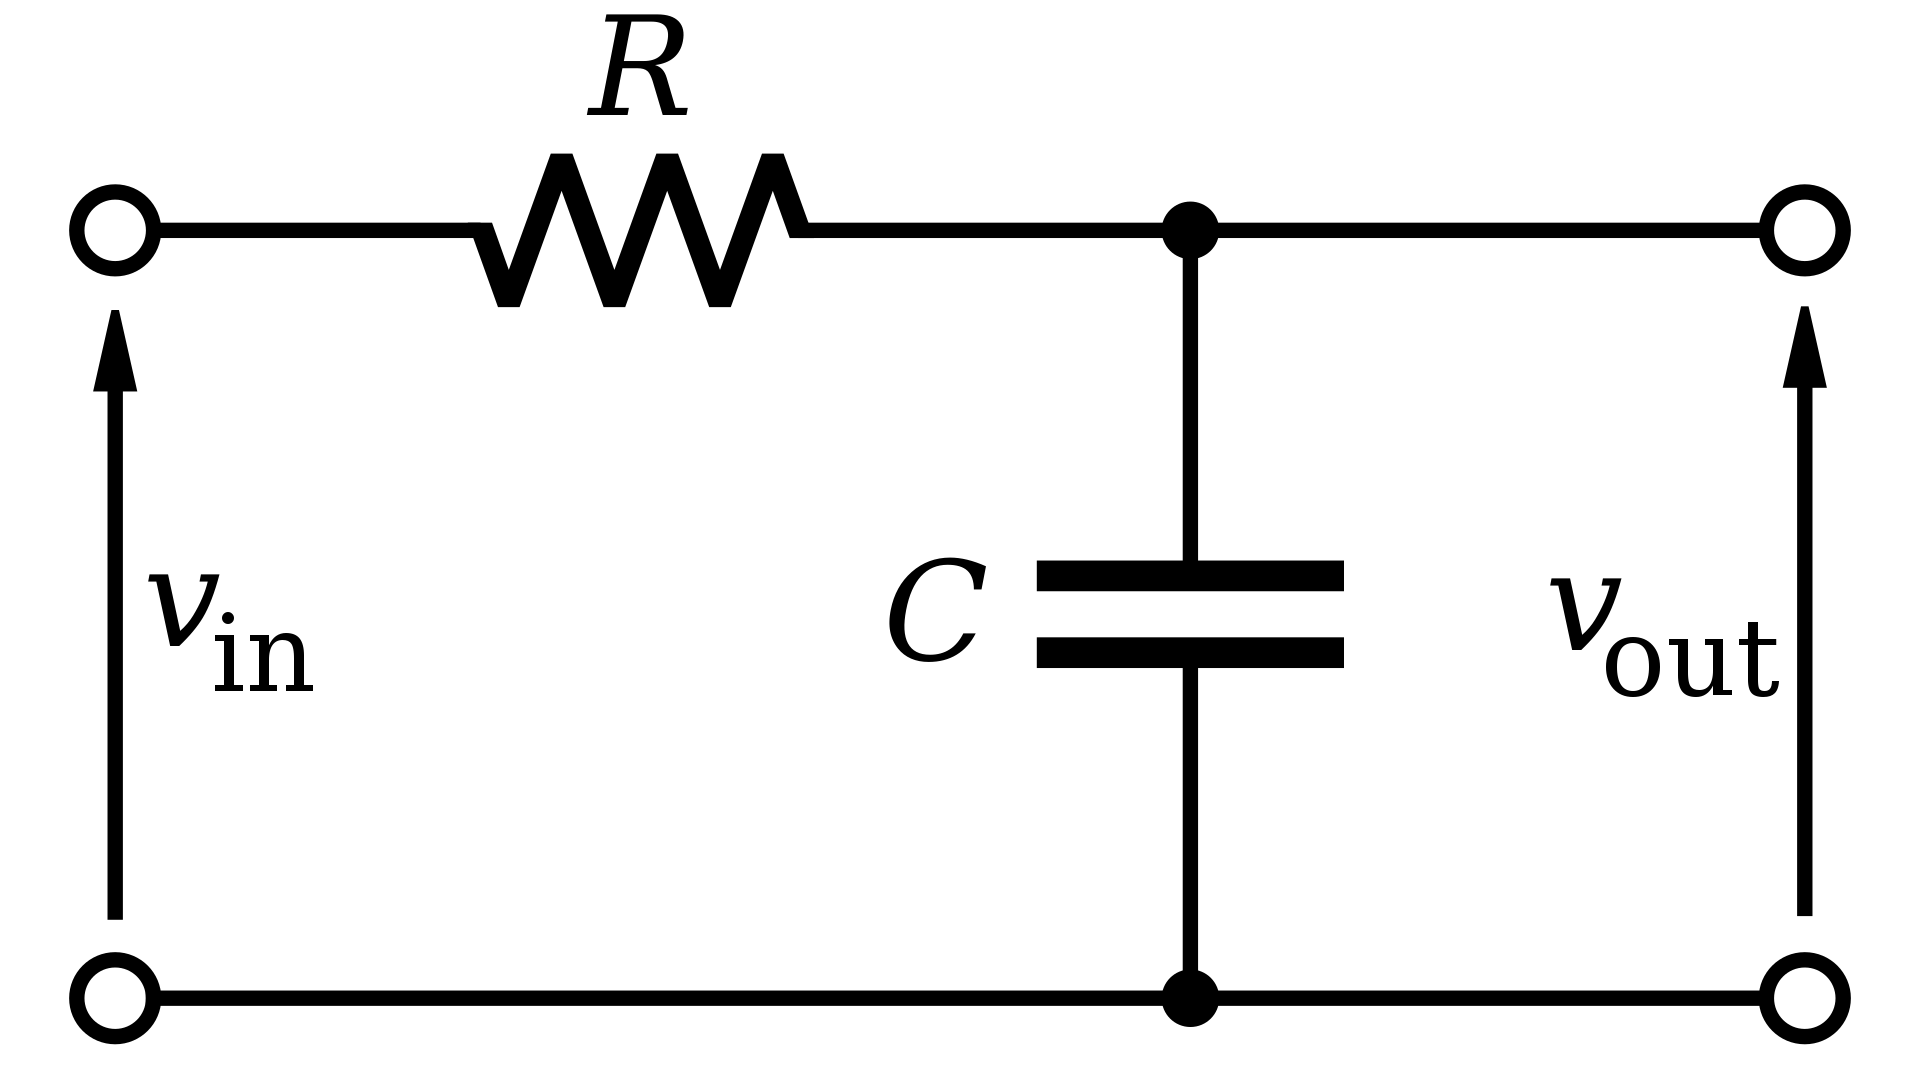
\includegraphics[width=4cm]{media/1st_Order_Lowpass_Filter_RC.png}
                \caption{Circuito filtro passa basso ideale}
                \label{fig:circuito filtro passa basso ideale}
            \end{figure}
            \[
                \frac{V_{out}}{V_{in}} = H_{(f)} = \frac{1}{1+j\frac{f}{f_T}},\ f_T = \frac{1}{2\pi RC}
            \] 
            Possiamo rappresentare in scala logaritmica il filtro: $\eval*{|H_{(f)}|}_{db} = 10log\left( \frac{\left|H_{(f)}\right|^2}{\left|H_{(f_0)}\right|^2} \right)$.
            Prendiamo la frequenza di riferimento $f_0: H_{(f_0)} = 1$
            \begin{figure}[H]
                \centering
                \begin{tikzpicture}
                    \begin{semilogxaxis}[
                        width=12cm,
                        xmin=0.01,
                        ymin=-20,
                        xmajorgrids=true,
                        ymajorgrids=true,
                        xlabel=$Frequenza$,
                        ylabel={Gain (db)},
                        ytick={0,-3,-5,-10,-15,-20},
                        yticklabels={$0$,$-3db$,$-5$,$-10$,$-15$,$-20$}
                    ] 
                        \addplot[domain=0.01:10000,samples=1000,color=blue]{20*log10(1/sqrt(1+(x/10)^2))};
                    \end{semilogxaxis}
                \end{tikzpicture}
                \caption{Filtro passa basso ideale in scala logaritmica}
                \label{fig:LP filter logartithm}
            \end{figure} 
            
            Otteniamo la Frequenza di taglio \index{Frequenza di taglio}$f_T$ all'ampiezza di $-3db$, in questo caso $f_T = 10$, alla quale
            il filtro "taglia" o meglio riduce tutte le ampiezze in ingresso verso lo 0.
            (To DO: controllare sul libro la formula per il calcolo di Hf)
            \begin{figure}[H]
                \centering
                \begin{tikzpicture}
                    \begin{semilogxaxis}[
                        width=12cm,
                        xmin = 0.01,
                        xmajorgrids=true,
                        ymajorgrids=true,
                        xlabel={Frequency (Hz)},
                        ylabel={Phase (degrees)},
                        ytick={-180,-135,-90,-45,0,45,90,135,180},
                        yticklabels={$-180$,$-135$,$-90$,$-45$,$0$,$45$,$90$,$135$,$180$}
                    ] 
                        \addplot[domain=0.01:10000,samples=1000,color=blue]{(atan(-x/10))};
                    \end{semilogxaxis}
                \end{tikzpicture}
                \caption{Filtro passa basso ideale fase}
                \label{fig:LP filter phase}
            \end{figure} 

            $Osservazione$: 
            \begin{itemize}
                \item{
                    Al tendere di $B$ a $0$ il valore che il filtro fa passare é il valor medio del segnale, tanto da tendere
                    a un filtro $LP$ con spettro $\delta_{(t)}$, ma é difficilmente realizzabile.
                }
                \item{
                    La banda di un filtro é quanto si estende da $0 \rightarrow f^+$ fino a arrivare a $B$,$[0,B]$
                }
                \item{
                    Se il filtro é un filtro $BP$ la banda é l'ampiezza della banda che lascia passare $[f_0-B,f_0+B] = B$
                }
            \end{itemize}
        \subsubsection{Filtro Passa Alto di banda B - High Pass Filter (HP)}\label{Filtro Passa Alto di banda B - High Pass Filter (HP)}
            \begin{figure}[H]
                \centering
                \begin{tikzpicture}
                    \begin{axis}[
                        domain=-5:5,
                        samples=200,
                        axis lines=middle,
                        xlabel=$f$,
                        ylabel=$H_{HP(f)}$,
                        xmax=5,
                        xmin=-5,
                        ymin=-0.3,
                        ymax=2.5,
                        xtick={-2,2},
                        xticklabels={$-B$,$B$},
                        ytick={},
                        yticklabels={},
                        width=9cm,
                        height=6cm
                    ]
                    \addplot [const plot,thick,orange] coordinates{(-5,1)(-2,1)};
                    \addplot [const plot,thick,orange] coordinates{(5,1)(2,1)};
                    \addplot [const plot,thick,orange] coordinates{(-2,0)(-2,1)};
                    \addplot [const plot,thick,orange] coordinates{(-2,0)(2,0)};
                    \addplot [const plot,thick,orange] coordinates{(2,1)(2,0)};
                    
                    \end{axis}
                \end{tikzpicture}

                \caption{Filtro passa alto ideale: Risposta in frequenza}
                \label{fig:filtro passa alto ideale}
            \end{figure}  
            
            \paragraph{Risposta in frequenza:}
            \[
                H_{HP(f)}\triangleq 1 - rect\left(\frac{f}{2B}\right)  
            \]
            \paragraph{Risposta impulsiva:}
            \[
                h_{HP(t)}\triangleq \delta_{(t)} - 2Bsinc(2Bt)  
            \]

        \paragraph{Cricuito Filtro Passa Alto:}
            \begin{figure}[H]
                \centering
                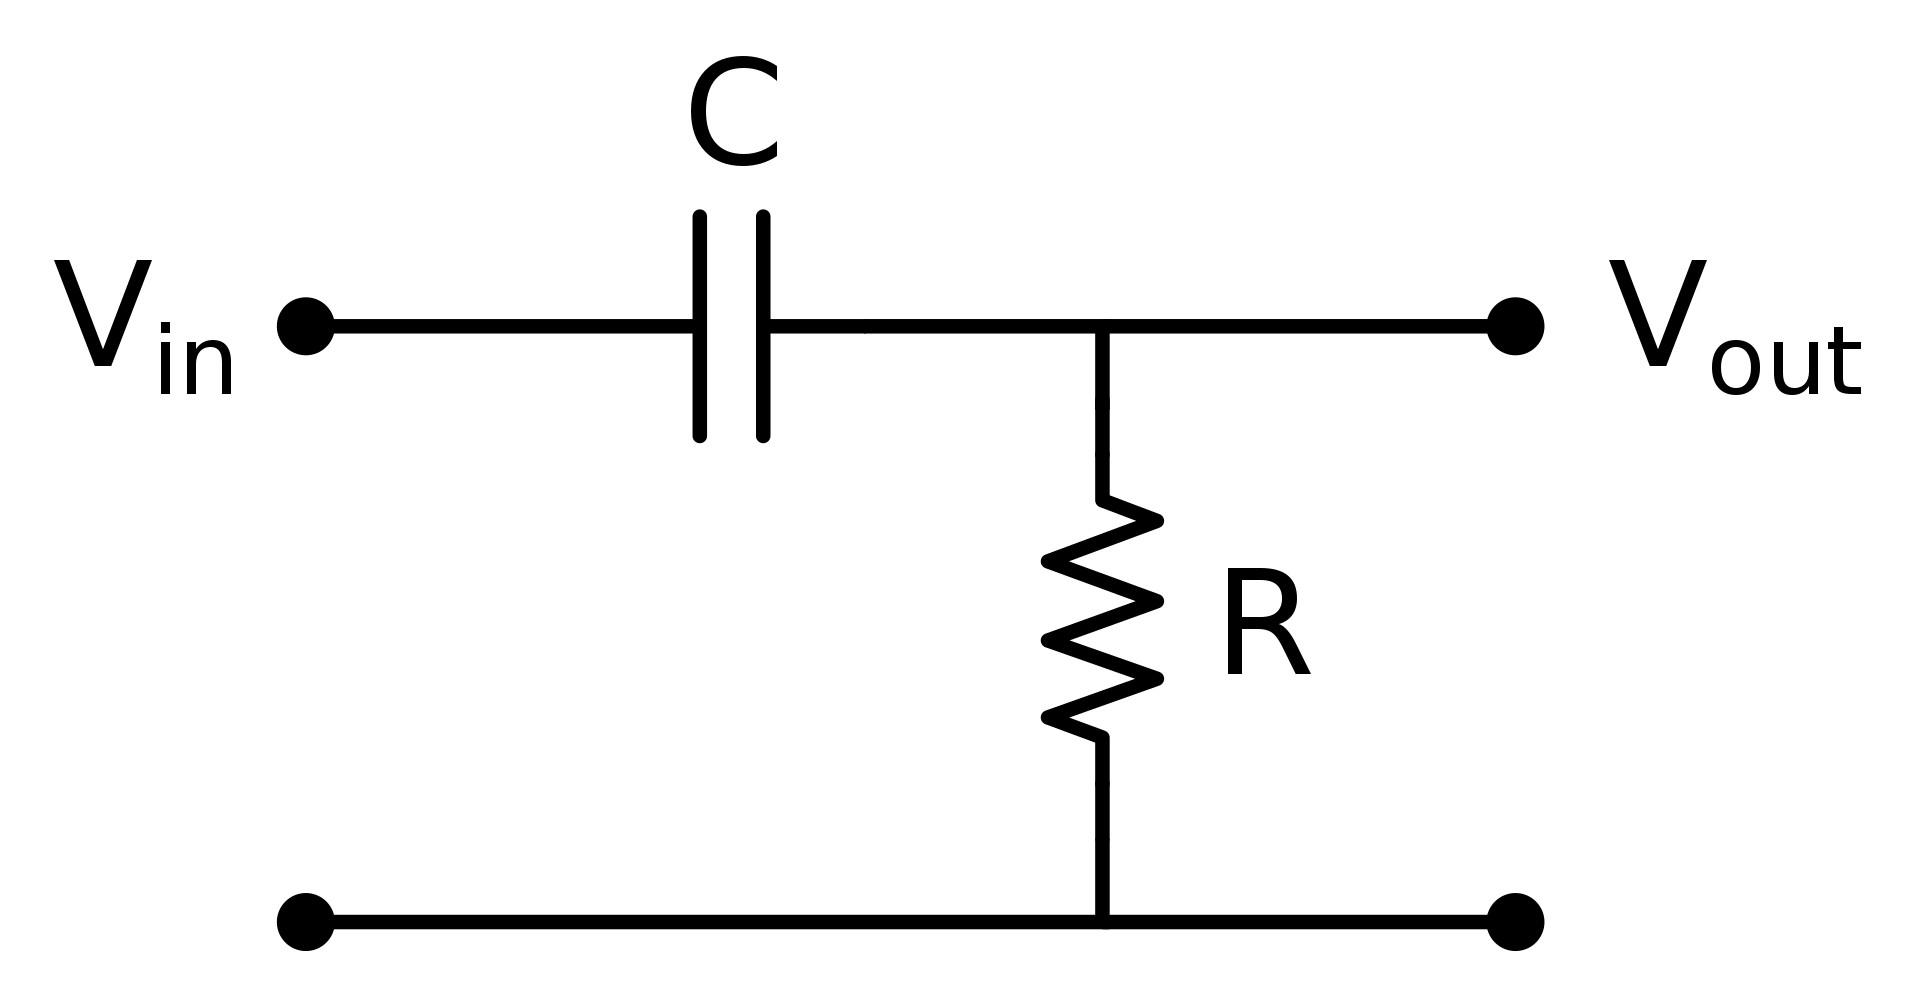
\includegraphics[width=4cm]{media/CR_high_pass_filter.png}
                \caption{Circuito filtro passa alto ideale}
                \label{fig:circuito filtro passa alto ideale}
            \end{figure}
            \[
                    H_{(f)} = \frac{fRC}{1+fRC}  
            \] 
        In scala logaritmica:
        \begin{figure}[H]
            \centering
            \begin{tikzpicture}
                \begin{semilogxaxis}[
                    width=12cm,
                    xmin=0.01,
                    ymin=-40,
                    xmajorgrids=true,
                    ymajorgrids=true,
                    xlabel=$Frequenza$,
                    ylabel={Gain (db)},
                    ytick={0,-3,-5,-10,-15,-20,-30,-40},
                    yticklabels={$0$,$-3db$,$-5$,$-10$,$-15$,$-20$,$-30$,$-40$}
                ] 
                    \addplot[domain=0.01:10000,samples=1500,color=blue]{20*log10(sqrt((x/10)^2)/sqrt(1+(x/10)^2))};
                \end{semilogxaxis}
            \end{tikzpicture}
            \caption{Filtro passa alto ideale in scala logaritmica}
            \label{fig:HP filter logartithm}
        \end{figure} 
        \begin{figure}[H]
            \centering
            \begin{tikzpicture}
                \begin{semilogxaxis}[
                    width=12cm,
                    xmin = 0.01,
                    xmajorgrids=true,
                    ymajorgrids=true,
                    xlabel={Frequency (Hz)},
                    ylabel={Phase (degrees)},
                    ytick={-180,-135,-90,-45,0,45,90,135,180},
                    yticklabels={$-180$,$-135$,$-90$,$-45$,$0$,$45$,$90$,$135$,$180$}
                ] 
                    \addplot[domain=0.01:10000,samples=1000,color=blue]{(atan(-x/10)+90)};
                \end{semilogxaxis}
            \end{tikzpicture}
            \caption{Filtro passa alto ideale fase}
            \label{fig:HP filter phase}
        \end{figure} 
        Si nota come avendo preso la $f_T$ corrisponde a $RC = 10$. 
        \subsubsection{Filtro Passa Banda di banda B - Band Pass Filter (BP)}\label{Filtro Passa Banda di banda B - Band Pass Filter (BP)}
            \begin{figure}[H]
                \centering
                \begin{tikzpicture}
                    \begin{axis}[
                        domain=-5:5,
                        samples=200,
                        axis lines=middle,
                        xlabel=$f$,
                        ylabel=$H_{BP(f)}$,
                        xmax=5,
                        xmin=-5,
                        ymin=-0.3,
                        ymax=1.5,
                        xtick={-4,-3,-2,2,3,4},
                        xticklabels={$-B-f_0$,$-f_0$,$B-f_0$,$B+f_0$,$f_0$,$B+f_0$},
                        ytick={},
                        xticklabel style={font=\tiny},
                        yticklabels={},
                        width=12cm,
                        height=6cm
                    ]
                    \addplot [const plot,thick,orange] coordinates{(-5,0)(-4,0)};
                    \addplot [const plot,thick,orange] coordinates{(-2,0)(2,0)};
                    \addplot [const plot,thick,orange] coordinates{(5,0)(4,0)};
                    \addplot [const plot,thick,orange] coordinates{(-4,0)(-4,1)};

                    \addplot [const plot,thick,orange] coordinates{(-4,1)(-2,1)};
                    \addplot [const plot,thick,orange] coordinates{(-2,0)(-2,1)};
                    
                    \addplot [const plot,thick,orange] coordinates{(4,1)(2,1)};
                    \addplot [const plot,thick,orange] coordinates{(2,0)(2,1)};
                    \addplot [const plot,thick,orange] coordinates{(4,0)(4,1)};
                    
                    \end{axis}
                \end{tikzpicture}
                \caption{Filtro passa banda ideale: Risposta in frequenza}
                \label{fig:filtro passa banda ideale}
            \end{figure} 
            
            \paragraph{Risposta in frequenza:}
            \[
                H_{BP(f)}\triangleq H_{LP(f+f_0)} +H_{LP(f-f_0)} =  rect\left(\frac{f-f_0}{2B}\right) + rect\left(\frac{f+f_0}{2B}\right)  
            \]
            \paragraph{Risposta impulsiva:}
            \[
                h_{BP(t)}\triangleq 2Bsinc(2Bt) \cos(2\pi f_0t) = h_{LP(t)}\cos(2\pi f_0t)   
            \]
            \begin{figure}[H]
                \centering

                \begin{tikzpicture}
                    \begin{axis}[
                        domain=-5:5,
                        samples=200,
                        axis lines=middle,
                        xlabel=$t$,
                        ylabel=$h_{LP(t)}$,
                        xmax=5,
                        xmin=-5,
                        ymin=-5,
                        ymax=5,
                        xtick={},
                        xticklabels={},
                        ytick={},
                        yticklabels={},
                        width=12cm
                    ]
                    \addplot [const plot,thick,orange, samples = 1000] {(2*(sin(deg((x)*pi))/((x)*pi)))*cos(deg(2*pi*10*x))};
                    \end{axis}
                \end{tikzpicture}

                \caption{Filtro passa banda: risposta impulsiva}
                \label{fig:filtro passa banda ideale causale}
            \end{figure} 

            \paragraph{Cricuito Filtro Passa Banda:}
                \begin{figure}[H]
                    \centering
                    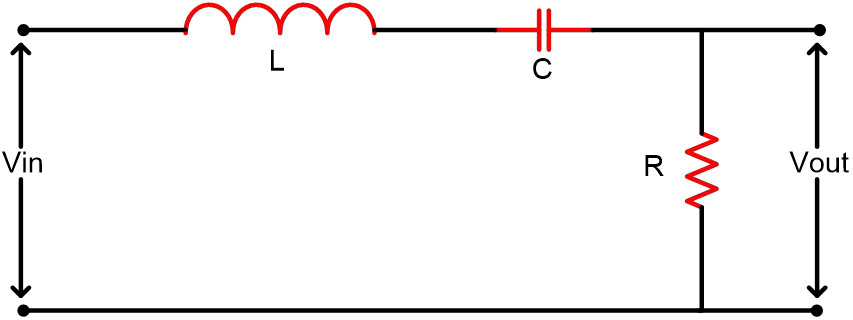
\includegraphics[width=4cm]{media/Band-Pass-Filter.png}
                    \caption{Circuito filtro passa banda ideale}
                    \label{fig:circuito filtro passa banda ideale}
                \end{figure} 
            In scala logaritmica:
            \begin{figure}[H]
                \centering
                \begin{tikzpicture}
                    \begin{semilogxaxis}[
                        width=12cm,
                        xmin=10^-1,
                        xmajorgrids=true,
                        ymajorgrids=true,
                        xlabel=$Frequenza$,
                        ylabel={Gain (db)},
                        ytick={0,-3,-5,-10,-15,-20},
                        yticklabels={$0$,$-3db$,$-5$,$-10$,$-15$,$-20$}
                    ] 
                        \addplot[domain=10^-1:10000,samples=1000,color=blue]{20*log10(abs(((200*x)/(x^2+100*x+2500))))};
                    \end{semilogxaxis}
                \end{tikzpicture}
                \caption{Filtro passa banda ideale in scala logaritmica}
                \label{fig:BP filter logartithm}
            \end{figure}
            Non riesco a fare un grafico con pendenza maggiore ma é per capire che le frequenze sotto il valore di $-3db$
            vengono ridotte drasticamente.
            \begin{figure}[H]
                \centering
                \begin{tikzpicture}
                    \begin{semilogxaxis}[
                        width=12cm,
                        xmin = 0.01,
                        xmajorgrids=true,
                        ymajorgrids=true,
                        xlabel={Frequency (Hz)},
                        ylabel={Phase (degrees)},
                        ytick={-180,-135,-90,-45,0,45,90,135,180},
                        yticklabels={$-180$,$-135$,$-90$,$-45$,$0$,$45$,$90$,$135$,$180$}
                    ] 
                        \addplot[domain=0.01:10000,samples=1000,color=blue]{(atan((x)/70))-180};
                    \end{semilogxaxis}
                \end{tikzpicture}
                \caption{Filtro passa banda ideale fase}
                \label{fig:BP filter phase}
            \end{figure} 
        \subsubsection{Filtro Elimina Banda di banda B - Band Stop Filter (BS)}\label{Filtro Elimina Banda di banda B - Band Stop Filter (BS)}
            \begin{figure}[H]
                \centering
                
                \begin{tikzpicture}
                    \begin{axis}[
                        domain=-5:5,
                        samples=200,
                        axis lines=middle,
                        xlabel=$f$,
                        ylabel=$H_{BS(f)}$,
                        xmax=5,
                        xmin=-5,
                        ymin=-0.3,
                        ymax=2.5,
                        xtick={-4,-3,-2,2,3,4},
                        xticklabels={$-B-f_0$,$-f_0$,$B-f_0$,$B+f_0$,$f_0$,$B+f_0$},
                        xticklabel style={font=\tiny},
                        ytick={},
                        yticklabels={},
                        width=9cm,
                        height=6cm
                    ]
                    \addplot [const plot,thick,orange] coordinates{(-5,1)(-4,1)};
                    \addplot [const plot,thick,orange] coordinates{(-2,1)(2,1)};
                    \addplot [const plot,thick,orange] coordinates{(5,1)(4,1)};
                    \addplot [const plot,thick,orange] coordinates{(-4,0)(-4,1)};

                    \addplot [const plot,thick,orange] coordinates{(-4,0)(-2,0)};
                    \addplot [const plot,thick,orange] coordinates{(-2,0)(-2,1)};
                    
                    \addplot [const plot,thick,orange] coordinates{(4,0)(2,0)};
                    \addplot [const plot,thick,orange] coordinates{(2,0)(2,1)};
                    \addplot [const plot,thick,orange] coordinates{(4,0)(4,1)};
                    
                    \end{axis}
                \end{tikzpicture}
                \caption{Filtro elimina banda ideale}
                \label{fig:filtro elimina banda ideale}
            \end{figure} 

            \paragraph{Risposta in frequenza:}
            \[
                H_{BS(f)}\triangleq 1 -(H_{BP(f+f_0)} +H_{BP(f-f_0)}) = 1- \left[ rect\left(\frac{f-f_0}{2B}\right) + rect\left(\frac{f+f_0}{2B}\right)\right]  
            \]
            \paragraph{Risposta impulsiva:}
            \[
                h_{BS(t)}\triangleq \delta_{(t)} - h_{BP(t)} = \delta_{(t)} - 2Bsinc(2Bt) \cos(2\pi f_0t)
            \]

            \paragraph{Cricuito Filtro Elimina Banda:}
                \begin{figure}[H]
                    \centering
                    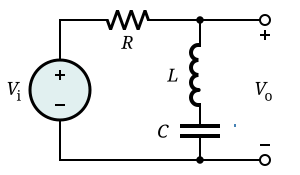
\includegraphics[width=4cm]{media/Band-Reject_Filter.png}
                    \caption{Circuito filtro elimina banda ideale}
                    \label{fig:circuito filtro elimina banda ideale}
                \end{figure}
                \[
                    H_{(f)} = \frac{}{}  
                \]
            In scala logaritmica:
            \begin{figure}[H]
                \centering
                \begin{tikzpicture}
                    \begin{semilogxaxis}[
                        width=12cm,
                        xmin=0.01,
                        ymin=-50,
                        xmajorgrids=true,
                        ymajorgrids=true,
                        xlabel=$Frequenza$,
                        ylabel={Gain (db)},
                        ytick={0,-3,-5,-10,-15,-20,-25,-30,-35,-40,-45},
                        yticklabels={$0$,$-3db$,$-5$,$-10$,$-15$,$-20$,$-25$,$-30$,$-35$,$-40$,$-45$}
                    ] 
                        \addplot[domain=0.01:10000,samples=1000,color=blue]{20*log10(abs(1-((200*x)/(x^2+100*x+2500))))};
                    \end{semilogxaxis}
                \end{tikzpicture}
                \caption{Filtro elimina banda ideale in scala logaritmica}
                \label{fig:BS filter logartithm}
            \end{figure}
            \begin{figure}[H]
                \centering
                \begin{tikzpicture}
                    \begin{semilogxaxis}[
                        width=12cm,
                        xmin = 0.01,
                        xmajorgrids=true,
                        ymajorgrids=true,
                        xlabel={Frequency (Hz)},
                        ylabel={Phase (degrees)},
                        ytick={-180,-135,-90,-45,0,45,90,135,180},
                        yticklabels={$-180$,$-135$,$-90$,$-45$,$0$,$45$,$90$,$135$,$180$}
                    ] 
                        \addplot[domain=0.01:10000,samples=1000,color=blue]{(atan(-(x)/70))};
                    \end{semilogxaxis}
                \end{tikzpicture}
                \caption{Filtro elimina banda ideale fase}
                \label{fig:BS filter phase}
            \end{figure} 
            Tutti i filtri possono essere ricavati dal filtro \textbf{Low-Pass} \ref{Filtro Passa Basso di banda B - Low Pass Filter (LP)}
            o dal filtro \textbf{High-Pass} \ref{Filtro Passa Alto di banda B - High Pass Filter (HP)}.

            I filtri sono riconducibili a funzioni di trasferimento come quelle viste per il tracciamento di Bode nel corso
            di fondamenti di automatica.
        \subsubsection{Filtri non distorcenti}
            Definiamo prima cos'é  un sengale non distorto:
            \begin{figure}[H]
                \centering
                \begin{tikzpicture}[
                    node distance=2cm,
                    >=latex
                    ]
    
                    \node [coordinate] (input) {};
                    \node [draw, rectangle,right of = input, minimum height=3em, minimum width=6em] (block) {$T[\ ]$};
                    \node [coordinate, right of = block] (output) {};
                    
                    \draw[draw,->] (input) -- node[above]{$x_{(t)}$} (block);
                    \draw[->] (block) -- node[above]{$y_{(t)}$} (output);
                \end{tikzpicture}
                \label{fig:Sistema non distorcente}
            \end{figure}
            {\color{blue}$y_{(t)}$} é un segnale non distorto di $x$ se: $y_{(t)}\triangleq kx_{(t-t_0)}$ $k\in\mathbb{R}^+$, cioé finché esso rimane una versione
            ritardata e/o amplificata del segnale $x_{(t)}$, in frequenza:
            \[
                Y_{(f)} = kX_{(f)}e^{-j2\pi ft_0}   
            \]
            \begin{figure}[H]
                \centering
                \begin{tikzpicture}
                    \begin{axis}[
                        domain=-0.3:15,
                        samples=200,
                        axis lines=middle,
                        xlabel=$t$,
                        ylabel=$y_{(t)}$,
                        xmax=6,
                        xmin=-0.3,
                        ymin=-0.3,
                        ymax=2.5,
                        xtick={5},
                        xticklabels={$t_0$},
                        ytick={},
                        yticklabels={},
                        width=12cm,
                        height=6cm
                    ]
                    \addplot [thick,orange, samples = 400, domain = 0:2] {-0.9*(x^2-2*x)+(0.1*cos(deg(25*x*pi)))};
                    \addplot [thick,blue, samples = 400, domain = 4:6] {-0.6*((x-4)*(x-6))+(0.1*cos(deg(25*x*pi)))};
                    
                    \end{axis}
                \end{tikzpicture}
                \label{fig:segnale non distorto}
            \end{figure} 
            

            \paragraph{Analisi del filtro non distorcente:}
            Come deve essere realizzato il filtro in modo tale da non distorcere il segnale?
            \[
                y_{(t)}=x_{(t)}\otimes h_{(t)} {\color{blue}=kx_{(t-t_0)}} 
            \]
            Per non essere distorcente la risposta impulsiva del sistema deve essere $k\delta_{(t-t_0)}$ con risposta in frequenza:
            $H_{(f)} = ke^{-j2\pi ft_0}$
            
            \begin{figure}[H]
                \centering
                \subfloat[Ampiezza con ritardo]{
                    \begin{tikzpicture}
                        \begin{axis}[
                            domain=-5:5,
                            samples=200,
                            axis lines=middle,
                            xlabel=$f$,
                            ylabel=$|H_{(f)}|$,
                            ytick = {1},
                            yticklabels = {$k$},
                            xtick = {},
                            yticklabel style = {yshift=6pt}, 
                            xticklabels = {},
                            ymin=-0.2,
                            ymax=1.5,
                            width=6cm,
                            height=4cm
                        ]
                        \addplot [const plot,blue, thick] coordinates{(-5,1)(5,1)};
                        \end{axis}
                    \end{tikzpicture}
                    \label{fig:Ampiezza filtro non distorcente}
                }
                \hfill
                \subfloat[Fase con ritardo]{
                        \begin{tikzpicture}
                            \begin{axis}[
                                domain=-5:5,
                                samples=200,
                                axis lines=middle,
                                xlabel=$f$,
                                ylabel=$\angle H_{(f)}$,
                                xmax=5,
                                xmin=-5,
                                xtick = {},
                                xticklabels = {},
                                ytick={},
                                yticklabel style = {yshift=6pt}, 
                                yticklabels={},
                                width=6cm,
                                height=5cm
                            ]
                            \addplot [blue, thick, samples = 300, domain = -4:4] {-x};
                            \addplot [blue, densely dashed] coordinates{(-4,4)(-5,5)};
                            \addplot [blue, densely dashed] coordinates{(4,-4)(5,-5)};
                            \end{axis}
                        \end{tikzpicture}
                    \label{fig:fase filtro non distorcente}
                }
                \caption{Spettro filtro non distorcente}
            \end{figure}
            Avere un tale filtro per tutti i segnali é molto restringente, ci basta che il nostro filtro sia non distorcente nella banda che ci interessa.
            
            \begin{figure}[H]
                \centering
                \subfloat[Ampiezza con ritardo]{
                    \begin{tikzpicture}
                        \begin{axis}[
                            domain=-5:5,
                            samples=1000,
                            axis lines=middle,
                            xlabel=$f$,
                            ylabel=$|H_{(f)}|$,
                            ytick = {1},
                            yticklabels = {$k$},
                            xtick = {-2,2},
                            yticklabel style = {yshift=6pt}, 
                            xticklabels = {$-B$,$B$},
                            ymin=-0.2,
                            ymax=1.5,
                            width=6cm,
                            height=4cm
                        ]
                        \addplot [dotted,blue, thick] coordinates{(-5,1)(5,1)};
                        \addplot [blue, thick, samples = 1000, restrict y to domain=0:1] {-(x/2)^2+1};
                        \addplot [dotted,orange, thick] coordinates{(-2,0)(-2,1)};
                        \addplot [dotted,orange, thick] coordinates{(2,0)(2,1)};
                        \addplot [dotted,orange, thick] coordinates{(-2,1)(2,1)};
                        \end{axis}
                    \end{tikzpicture}
                    \label{fig:Ampiezza filtro non distorcentein banda}
                }
                \hfill
                \subfloat[Fase con ritardo]{
                        \begin{tikzpicture}
                            \begin{axis}[
                                domain=-5:5,
                                samples=200,
                                axis lines=middle,
                                xlabel=$f$,
                                ylabel=$\angle H_{(f)}$,
                                xmax=5,
                                xmin=-5,
                                ymin=-3,
                                ymax=3,
                                xtick = {-2,2},
                                xticklabels = {$-B$,$B$},
                                ytick={},
                                yticklabel style = {yshift=6pt}, 
                                yticklabels={},
                                width=6cm,
                                height=5cm
                            ]
                            \addplot [blue, dotted, samples = 300, domain = -5:5] {-x};
                            \addplot [blue, thick, samples = 300, domain = -2:2] {-x};
                            \addplot [blue, thick] coordinates{(-2,2)(-5,2)};
                            \addplot [blue, dotted,thick] coordinates{(-2,2)(-2,0)};
                            \addplot [blue, thick] coordinates{(2,-2)(5,-2)};
                            \addplot [blue, dotted,thick] coordinates{(2,-2)(2,0)};
                            \end{axis}
                        \end{tikzpicture}
                    \label{fig:fase filtro non distorcente in banda}
                }
                \caption{Spettro filtro non distorcente limitato alla banda $B$}
            \end{figure}            
            Il filtro ci basta che sia qualcosa che si avvicini a una $rect$ ad esempio un coseno rialzato \ref{F. Coseno Rialzato}

    \subsection{Th. di Parseval}\label{Th. di Parseval}
        \[
              E_{x} = \int_{-\infty}^{\infty}|x_{(t)}|^2 dt = \int_{-\infty}^{\infty}|X_{(f)}|^2 df =\int_{-\infty}^{\infty} S_{x(f)} df
        \]
        $S_{x(f)} = |X_{(f)}|^2$ é la densitá spettrale di energia del segnale, ci mostra come l'energia é distribuita nello spettro.
        
        Dimostrazione:
        \begin{align}
            E_{x} &= \int_{-\infty}^{\infty}|x_{(t)}|^2 dt =\int_{-\infty}^{\infty}x_{(t)}x_{(t)}^{\star} dt = \int_{-\infty}^{\infty}x_{(t)}\left[\int_{-\infty}^{\infty}X_{(f)}e^{j2\pi ft}df\right]^\star dt\nonumber \\
                  &= \underset{(t)}{\int_{-\infty}^{\infty}}x_{(t)}\underset{(f)}{\int_{-\infty}^{\infty}}X_{(f)}^\star e^{-j2\pi ft}dfdt = \underset{(f)}{\int_{-\infty}^{\infty}}X_{(f)}^\star\underset{(t)}{\int_{-\infty}^{\infty}}x_{(t)} e^{-j2\pi ft}dtdf \nonumber \\
                  &= \int_{-\infty}^{\infty}X_{(f)}^\star X_{(f)} df = \int_{-\infty}^{\infty}|X_{(f)}|^2 df\nonumber
        \end{align}
        Come capisco quanta \% del segnale sto buttando?

        \begin{figure}[H]
            \centering
            \begin{tikzpicture}
                \begin{axis}[
                    domain=-3:3,
                    samples=1000,
                    axis lines=middle,
                    xlabel=$f$,
                    ylabel=$|S_{x(f)}|$,
                    ytick = {},
                    yticklabels = {},
                    xtick = {-1.3,1.3},
                    yticklabel style = {yshift=6pt}, 
                    xticklabels = {$-B$,$B$},
                    ymin=-0.2,
                    ymax=1.5,
                    width=6cm,
                    height=4cm
                ]
                \addplot [blue, thick] {exp(-x^2)};
                \addplot [name path = A,domain=-3:-1.3,blue, thick] {exp(-x^2)};
                \addplot [name path = B,domain=1.3:3,blue, thick] {exp(-x^2)};
                \addplot [dotted,blue,thick] coordinates{(-1.3,0)(-1.3,0.15)};
                \addplot [dotted,blue,thick] coordinates{(1.3,0)(1.3,0.15)};
                \addplot [const plot,name path = C,black, thin] coordinates{(-1.3,0)(-3,0)};
                \addplot [const plot,name path = D,black, thin] coordinates{(1.3,0)(3,0)};

                \addplot[green,opacity = 0.5] fill between[of=A and C];
                \addplot[green,opacity = 0.5] fill between[of=B and D];

                \end{axis}
            \end{tikzpicture}
            \caption{Spettro $S_{x(f)}$}
        \end{figure}            
        \noindent La parte {\color{green}verde} é l'energia del segnale che perdiamo troncandolo con banda $B$
    \subsection{Funzione di Correlazione - Segnali Aperiodici}\label{Funzione di Correlazione - Segnali Aperiodici}
        \[
            C_{xy} = R_{xy(\tau)}=\int_{-\infty}^{\infty}x_{(t)}y_{(t-\tau)}^\star dt 
        \]
    \subsection{Funzione di Autocorrelazione}\label{Funzione di Autocorrelazione}
        \[
            C_x = R_{x(\tau)}=\int_{-\infty}^{\infty}x_{(t)}x_{(t-\tau)}^\star dt 
        \]
        \noindent Misura la correlazione del segnale con se stesso.
        \subsubsection{Propietá Autocorrelazione}
            \begin{itemize}
                \item {$R_{x(0)} = E_x$
                    \[
                        R_{x(0)} =\int_{-\infty}^{\infty}x_{(t)}x_{(t)}^\star dt =\int_{-\infty}^{\infty}|x_{(t)}|^2 dt = E_x   
                    \]
                }
                \item {Simmetria Hermitiana:
                    \[
                        R_{x(-\tau)} =R_{x(\tau)}^\star 
                    \]
                }
                \item {$TCF$ Autocorrelazione:
                    \[ 
                        R_{x(\tau)} \overunderset{TCF}{ATCF}{\rightleftharpoons} S_{x(f)}
                    \]
                    Posso calcolare la densitá spettrale di energia dall'autocorrelazione.
                }
            \end{itemize}

    \section{Trasformata Discreta di Fourier}
    Si definisce Trasformata Discreta di Fourier:
    \begin{gather}
        x_{[nT]} \overunderset{TDF}{ATDF}{\rightleftharpoons} \overline{X}_{(f)} \nonumber \\
        \overline{X}_{(f)} \in \mathbb{C}: \begin{cases}
            \left| \overline{X}_{(f)} \right| \nonumber \\
            \angle \overline{X}_{(f)} \nonumber
        \end{cases} \text{é una funzione periodica di periodo }\frac{1}{T}\nonumber  
    \end{gather}
    \subsubsection{Equazione di Analisi - $TDF$} \label{TDF}
        \[
            \overline{X}_{(f)} = \sum_{n=-\infty}^{\infty} x_{[nT]}e^{-j2\pi fnT}
        \]
    \subsubsection{Equazione di Sintesi - $ATDF$} \label{ATDF}
        \[
            x_{[nT]} = \frac{1}{2\pi} \int_{2\pi} \overline{X}_{(f)}e^{j2\pi fnT} df
        \]
    \subsubsection{Trasformata di $\delta_{[n]}$}\label{tdf sequenza di delta}
        \begin{gather}
            \sum_{n=-\infty}^{\infty}\delta_{(t-nT)} \overset{\ref{prima formula di poisson}}{=} \frac{1}{T} \sum_{k=-\infty}^{\infty} \Delta_{(\frac{k}{T})}e^{-j2\pi \frac{k}{T}t} \overset{\Delta \text{ costante}}{=} \frac{1}{T} \sum_{k=-\infty}^{\infty} e^{-j2\pi \frac{k}{T}t} \nonumber \\
            \Downarrow TCF\nonumber \\
            \sum_{n=-\infty}^{\infty}e^{-j2\pi fnT} = \frac{1}{T} \sum_{k=-\infty}^{\infty} \delta_{(f-\frac{k}{T})}\nonumber
        \end{gather}
        Applicando il ritardo:
        \[
            \sum_{n=-\infty}^{\infty}e^{-j2\pi (f-\nu)nT} = \frac{1}{T} \sum_{k=-\infty}^{\infty} \delta_{((f-\nu)-\frac{k}{T})}
        \]
    \subsubsection{Relazione tra $TCF$ e $TDF$}\label{Relazione tra $TCF$ e $TDF$}
        \begin{align}
            \overline{X}_{(f)} &= \sum_{n=-\infty}^{\infty} x_{[nT]}e^{-j2\pi fnT} = \sum_{n=-\infty}^{\infty} \underset{(\nu)}{\int_{-\infty}^{\infty}} X_{(\nu)} e^{-j2\pi \nu nT} d\nu e^{-j2\pi fnT} \nonumber \\
                               &= \underset{(\nu)}{\int_{-\infty}^{\infty}} X_{(\nu)} \sum_{n=-\infty}^{\infty} e^{-j2\pi \nu nT} e^{-j2\pi fnT} d\nu \overset{\ref{tdf sequenza di delta}}{=} \underset{(\nu)}{\int_{-\infty}^{\infty}} X_{(\nu)} \sum_{n=-\infty}^{\infty} \frac{1}{T} \delta_{((f-\nu)-\frac{k}{T})} d\nu  \nonumber \\
                               &\overset{\ref{Propietá del Delta di Dirac}:\text{paritá}}{=} \underset{(\nu)}{\int_{-\infty}^{\infty}} X_{(\nu)} \frac{1}{T} \sum_{n=-\infty}^{\infty}  \delta_{(\nu-(f-\frac{k}{T}))} d\nu = \frac{1}{T} \sum_{n=-\infty}^{\infty} \underset{(\nu)}{\int_{-\infty}^{\infty}} X_{(\nu)} \delta_{(\nu-(f-\frac{k}{T}))} d\nu  \nonumber \\
                               &\overset{\ref{Propietá del Delta di Dirac}:\text{campionatrice}}{=}  \frac{1}{T} \sum_{n=-\infty}^{\infty} X_{(f-\frac{k}{T})} \nonumber
        \end{align}
        quindi la $TDF$ si ottiene periodicizzando la $TCF$ con periodo $\frac{1}{T}$:
        \[
            \overline{X}_{(f)} = \frac{1}{T} \sum_{n=-\infty}^{\infty} X_{(f-\frac{k}{T})} 
        \] 
        \begin{figure}[H]
            \centering
            \begin{tikzpicture}
                \begin{axis}[
                    domain=-15:15,
                    samples=200,
                    axis lines=middle,
                    xlabel=$f$,
                    ylabel=$X_{(f)}$,
                    ymin=-0.3,
                    ymax=1.5,
                    xtick={-8,-2.5,2.5,8},
                    xticklabels={$-\frac{1}{T}$,$-B$,$B$,$\frac{1}{T}$},
                    ytick={},
                    yticklabels={},
                    width=12cm,
                    height=5cm
                ]

                \addplot [thick,black, samples = 800] {exp(-x^2)};
                \addplot [ultra thick,blue, domain = -11:-5, samples = 800] {exp(-(x+8)^2)};
                \addplot [ultra thick,blue, domain = 5:11, samples = 800] {exp(-(x-8)^2)};

                \addplot [densely dashed,very thick,green, domain = -2.5:2.5, samples = 900] {exp(-x^2)};
                \addplot [densely dashed,very thick,green, domain = -11:-5, samples = 800] {exp(-(x+8)^2)};
                \addplot [densely dashed,very thick,green, domain = 5:11, samples = 800] {exp(-(x-8)^2)};
                \addplot [densely dashed,very thick,green] coordinates{(-11,0)(-15,0)};
                \addplot [densely dashed,very thick,green] coordinates{(11,0)(15,0)};
                \addplot [densely dashed,very thick,green] coordinates{(-2,0)(-5,0)};
                \addplot [densely dashed,very thick,green] coordinates{(2,0)(5,0)};

                \end{axis}
            \end{tikzpicture}
            \caption{${\color{black} X_{(f)}}$,${\color{blue} X_{(f-\frac{k}{T})}}$,${\color{green} \overline{X}_{(f)}}$}
            \label{fig:relazione tdf tcf}
        \end{figure}
    \subsection{Teorema del Campionamento - Nyquist Shannon}\label{Teorema del Campionamento - Nyquist Shannon}
        \begin{figure}[H]
            \centering
                \begin{tikzpicture}[
                        node distance=3cm,
                        >=latex
                    ]
                    % Blocks
                    \node [coordinate] (input) {};
                    \node [rectangle, draw,minimum height=2em, minimum width=4em,right of=input] (AD) {$A/D$};
                    \node [rectangle, draw,minimum height=2em, minimum width=4em,right of=AD] (DA) {$D/A$};
                    \node [coordinate,right of=DA] (output) {};
                
                    % Connections
                    \draw [->] (input) --node[above]{$x_{(t)}$} (AD);
                    \draw [->] (AD) --node[above]{$x_{[nT]}$} (DA);
                    \draw [->] (DA) --node[above]{$\hat{x}_{(t)}$} (output);
                \end{tikzpicture}    
            \label{fig:Sistema di campionamento e ricostruzione}
            \caption{Esempio sistema campionamento e ricostruzione}
        \end{figure}
        \begin{itemize}
            \item {
                A/D: Campionatore, converte da analogico a discreto.
            }
            \item {
                A/D: interpolatore o filtro $p$, converte da discreto a analogico.
            }
        \end{itemize}
        Il nostro obbiettivo é dimensionare T e l'interpolatore in modo tale da poter ricostruire il segnale $\hat{x}:\ \hat{x} =x$.
        \paragraph{Dimensioniamo l'$A/D$:} Riprendiamo la relazione tra $TDF$ e $TCF$:
        \begin{figure}[H]
            \centering
            \begin{tikzpicture}
                \begin{axis}[
                    domain=-15:15,
                    samples=200,
                    axis lines=middle,
                    xlabel=$f$,
                    ylabel=$X_{(f)}$,
                    ymin=-0.3,
                    ymax=1.5,
                    xtick={-8,-2.5,2.5,8},
                    xticklabels={$-\frac{1}{T}$,$-B$,$B$,$\frac{1}{T}$},
                    ytick={},
                    yticklabels={},
                    width=12cm,
                    height=5cm
                ]
                
                \addplot [thick,black, samples = 800] {exp(-x^2)};
                \addplot [ultra thick,blue, domain = -11:-5, samples = 800] {exp(-(x+8)^2)};
                \addplot [ultra thick,blue, domain = 5:11, samples = 800] {exp(-(x-8)^2)};

                \addplot [densely dashed,very thick,green, domain = -2.5:2.5, samples = 900] {exp(-x^2)};
                \addplot [densely dashed,very thick,green, domain = -11:-5, samples = 800] {exp(-(x+8)^2)};
                \addplot [densely dashed,very thick,green, domain = 5:11, samples = 800] {exp(-(x-8)^2)};
                \addplot [densely dashed,very thick,green] coordinates{(-11,0)(-15,0)};
                \addplot [densely dashed,very thick,green] coordinates{(11,0)(15,0)};
                \addplot [densely dashed,very thick,green] coordinates{(-2,0)(-5,0)};
                \addplot [densely dashed,very thick,green] coordinates{(2,0)(5,0)};

                \end{axis}
            \end{tikzpicture}
            \caption{${\color{black} X_{(f)}}$,${\color{blue} X_{(f-\frac{k}{T})}}$,${\color{green} \overline{X}_{(f)} = \frac{1}{T}\sum_{k=-\infty}^{\infty}X_{(f-\frac{k}{T})}}$}
            \label{fig:relazione tdf tcf campionamento f 2B}
        \end{figure}

        abbiamo trovato che la $TDF$  non é altro che la periodicizzazione della $TCF$ con periodo $\frac{1}{T}$: se $\frac{1}{T}\geq 2B$
        il grafico ${\color{blue} X_{(f-\frac{k}{T})}}$ sono copie distinte non distorte e periodicizzate di $X_{(f)}$ da cui con un Filtro Passa-Basso \ref{Filtro Passa Basso di banda B - Low Pass Filter (LP)} 
        possiamo ricostruire il segnale. Se scegliessi $\frac{1}{T}<2B$:
        \begin{figure}[H]
            \centering
            \begin{tikzpicture}
                \begin{axis}[
                    domain=-15:15,
                    samples=200,
                    axis lines=middle,
                    xlabel=$f$,
                    ylabel=$X_{(f)}$,
                    ymin=-0.3,
                    ymax=1.5,
                    xtick={-9,-6,-3,-2.5,2.5,3,9,6},
                    xticklabels={$-\frac{3}{T}$,$-\frac{2}{T}$,$-\frac{1}{T}$,$-B$,$B$,$\frac{1}{T}$,$\frac{3}{T}$,$\frac{2}{T}$,},
                    xticklabel style={font = \small,scale = 0.7},
                    ytick={},
                    yticklabels={},
                    width=12cm,
                    height=5cm
                ]
                
                \addplot [thick,black, samples = 800] {exp(-x^2)};
                \addplot [thick,blue, domain = -6:0, samples = 800] {exp(-(x+3)^2)};
                \addplot [thick,blue, domain = 0:6, samples = 800] {exp(-(x-3)^2)};

                \addplot [thick,blue, domain = -9:-3, samples = 800] {exp(-(x+6)^2)};
                \addplot [thick,blue, domain = 3:9, samples = 800] {exp(-(x-6)^2)};

                \addplot [thick,blue, domain = -11:-6, samples = 800] {exp(-(x+9)^2)};
                \addplot [thick,blue, domain = 6:11, samples = 800] {exp(-(x-9)^2)};

                \addplot [thick,green , samples = 800] {0.3*cos(deg(2.1*x))+0.7};

                \end{axis}
            \end{tikzpicture}
            \caption{${\color{black} X_{(f)}}$,${\color{blue} X_{(f-\frac{k}{T})}}$,${\color{green} \overline{X}_{(f)} = \frac{1}{T}\sum_{k=-\infty}^{\infty}X_{(f-\frac{k}{T})}}$}
            \label{fig:relazione tdf tcf campionamento f sbagliata}
        \end{figure}
        ho sovrapposizione delle copie di $X_{(f)}$ é il fenomeno di Aliasing: ho sovrapposizione di segnali che alterano il segnale originale. 
        In entrambi i casi ci troviamo in condizione di un segnale a banda limitata, nel tempo rappresenta un segnale illimitato.
        \paragraph{Dimensioniamo il $D/A$:}
        Partiamo dalla relazione di $\hat{x}$:
        \[
            \hat{x} = \sum_{n=-\infty}^{\infty}x_{[nT]}p_{(t-nT)},\ p\text{ interpolatore}
        \]
        Il segnale di uscita dal sistema dipende non solo dal periodo di campionamento $\frac{1}{T}$ ma anche dall'interpolatore che utilizziamo:
        \begin{itemize}
            \item {Interpolatore a mantenimento: mantiene il valore del segnale $x_{[nT]}$ per un periodo $T$
                \begin{figure}[H]
                    \centering
                    \begin{tikzpicture}
                        \begin{axis}[
                            domain=-5:5,
                            samples=200,
                            axis lines=middle,
                            xlabel=$t$,
                            ylabel=$p_{(t)}$,
                            ymin=-0.3,
                            ymax=5,
                            xmax=5,
                            xtick={3},
                            xticklabels={$T$},
                            ytick={1.5},
                            width=9cm,
                            height=4.5cm
                        ]
                        %x(t)
                        \addplot [const plot, thick, orange] coordinates{(0,0)(0,1.5)(3,1.5)(3,0)};
                        %Colors
                        \end{axis}
                    \end{tikzpicture}
                    \caption{Interpolatore a mantenimento}
                    \label{fig:interpolatore a mantenimento}
                \end{figure}
                \begin{figure}[H]
                    \centering
                    \begin{tikzpicture}
                        \begin{axis}[
                            domain=-5:5,
                            samples=200,
                            axis lines=middle,
                            xlabel=$t$,
                            ylabel=$x_{(t)}$,
                            ymin=-0.3,
                            ymax=5,
                            xtick={},
                            xticklabels={},
                            ytick={},
                            yticklabels={},
                            width=12cm,
                            height=5cm
                        ]
                        %x(t)
                        \addplot [thick,black, samples = 1000] {(x/3*sin(deg(6*x))+1.5)*((x/20)+1)};
                        \addplot [const plot,thick,orange, samples = 20] {(x/3*sin(deg(6*x))+1.5)*((x/20)+1)};
                        \addplot+ [ycomb, mark = none, dotted, black, samples = 20] {(x/3*sin(deg(6*x))+1.5)*((x/20)+1)};
                        %Colors
                        \end{axis}
                    \end{tikzpicture}
                    \caption{$x_{(t)}$,{\color{orange}$\hat{x} = \sum_{n=-\infty}^{\infty}x_{[nT]}p_{(t-nT)}$}}
                    \label{fig:x con interpolatore a mantenimento}
                \end{figure}
            }
            \item {Interpolatore Lineare: incrementa linearmente il valore di $\hat{x}$
                \begin{figure}[H]
                    \centering
                    \begin{tikzpicture}
                        \begin{axis}[
                            domain=-5:5,
                            samples=200,
                            axis lines=middle,
                            xlabel=$t$,
                            ylabel=$p_{(t)}$,
                            ymin=0.3,
                            xmin=-5,
                            ymax=5,
                            xmax=5,
                            xtick={-1.7,1.7},
                            xticklabels={$-\frac{T}{2}$,$\frac{T}{2}$},
                            ytick={2},
                            yticklabels={$1$},
                            width=9cm,
                            height=5cm
                        ]
                        \addplot [sharp plot,thick,orange] coordinates{(-2,0)(0,2)(2,0)};
                        \end{axis}
                    \end{tikzpicture}
                    \caption{Interpolatore Lineare}
                    \label{fig:interpolatore Lineare}
                \end{figure}
                \begin{figure}[H]
                    \centering
                    \begin{tikzpicture}
                        \begin{axis}[
                            domain=-5:5,
                            samples=200,
                            axis lines=middle,
                            xlabel=$t$,
                            ylabel=$x_{(t)}$,
                            ymin=-0.3,
                            ymax=5,
                            xtick={},
                            xticklabels={},
                            ytick={},
                            yticklabels={},
                            width=12cm,
                            height=5cm
                        ]
                        
                        \addplot [thick,black, samples = 1000] {(x/3*sin(deg(6*x))+1.5)*((x/20)+1)};
                        \addplot [sharp plot,thick,orange, samples = 20] {(x/3*sin(deg(6*x))+1.5)*((x/20)+1)};
                        \addplot+ [ycomb, mark = none, dotted, black, samples = 20] {(x/3*sin(deg(6*x))+1.5)*((x/20)+1)};
                        \end{axis}
                    \end{tikzpicture}
                    \caption{$x_{(t)}$,{\color{orange}$\hat{x} = \sum_{n=-\infty}^{\infty}x_{[nT]}p_{(t-nT)}$}}
                    \label{fig:x con interpolatore Lineare}
                \end{figure}
            }
        \end{itemize}
        Passiamo alla frequenza:
        \[
            \hat{x} = \sum_{n=-\infty}^{\infty}x_{[nT]}p_{(t-nT)} \overset{TCF}{\rightleftharpoons} \hat{X}_{(f)} = \sum_{n=-\infty}^{\infty}x_{[nT]}P_{(f)}e^{-j2\pi fnT}
        \]
        \begin{gather}
            \hat{X}_{(f)} = P_{(f)}\sum_{n=-\infty}^{\infty}x_{[nT]}e^{-j2\pi fnT} = P_{(f)}\overline{X}_{(f)} \nonumber \\
            Se\ \hat{x}=x\ anche\ \hat{X}_{(f)} = X_{(f)}\nonumber \\
            \Downarrow \ref{Relazione tra $TCF$ e $TDF$} \nonumber \\
            X_{(f)} \overset{!}{=} P_{(f)}\frac{1}{T}\sum_{k=-\infty}^{\infty}X_{(f-\frac{k}{T})} \nonumber
        \end{gather}
        dobbiamo dimensionare $P_{(f)}$ in modo tale da rendere vera $\hat{X}_{(f)} = X_{(f)}$
        \begin{figure}[H]
            \centering
            \begin{tikzpicture}
                \begin{axis}[
                    domain=-12:12,
                    samples=200,
                    axis lines=middle,
                    xlabel=$f$,
                    ylabel=$X_{(f)}$,
                    ymin=-0.3,
                    ymax=2,
                    xmax=12,
                    xmin=-12,
                    xtick={-8,-4,-3.2,-2.5,2.5,3.2,4,8},
                    xticklabels={$-\frac{1}{T}$,$-\frac{1}{2T}$,$-\frac{1}{3T}$,$-B$,$B$,$\frac{1}{3T}$,$\frac{1}{2T}$,$\frac{1}{T}$},
                    xticklabel style={font = \small,scale = 0.7},
                    ytick={},
                    yticklabels={},
                    width=12cm,
                    height=8cm 
                ]
                
                \addplot [thick,black, samples = 800] {0.5*exp(-x^2)};
                \addplot [ultra thick,blue, domain = -11:-5, samples = 800] {0.5*exp(-(x+8)^2)};
                \addplot [ultra thick,blue, domain = 5:11, samples = 800] {0.5*exp(-(x-8)^2)};

                \addplot [densely dashed,very thick,green, domain = -2.5:2.5, samples = 900] {0.5*exp(-x^2)};
                \addplot [densely dashed,very thick,green, domain = -11:-5, samples = 800] {0.5*exp(-(x+8)^2)};
                \addplot [densely dashed,very thick,green, domain = 5:11, samples = 800] {0.5*exp(-(x-8)^2)};
                
                \addplot [densely dashed,very thick,green] coordinates{(-11,0)(-15,0)};
                \addplot [densely dashed,very thick,green] coordinates{(11,0)(15,0)};
                \addplot [densely dashed,very thick,green] coordinates{(-2,0)(-5,0)};
                \addplot [densely dashed,very thick,green] coordinates{(2,0)(5,0)};

                \addplot [const plot, thick,orange] coordinates{(-3.2,0)(-3.2,0.6)(3.2,0.6)(3.2,0)};
                \addplot [const plot, dashed ,thick,orange] coordinates{(-11.2,0)(-11.2,0.6)(-4.8,0.6)(-4.8,0)};
                \addplot [const plot, dashed ,thick,orange] coordinates{(4.8,0)(4.8,0.6)(11.2,0.6)(11.2,0)};

                \end{axis}
            \end{tikzpicture}
            \caption{${\color{black} X_{(f)}}$,${\color{blue} X_{(f-\frac{k}{T})}}$,${\color{orange} P_{(f)}}$}
            \label{fig:tdf tcf dimansionamento interpolatore}
        \end{figure}
        Utilizziamo un filtro passa basso che abbia una durata in banda maggiore di $2B$ ma minore di $\frac{1}{2T}$  per lasciarci un pochino di margine e evitare di prendere 
        la copia del segnale successivo/precedente ($2B<T_r\leq\frac{1}{2T_s}$): prendiamo una durata $\frac{1}{2T_s}>2B$
        \[
            P_{(f)} = T rect\left(\frac{f}{2\frac{1}{2T}}\right)= T rect\left(fT\right) \overset{TCF}{\leftrightharpoons} p_{(t)} = \frac{T}{T}sinc\left(\frac{t}{T}\right)
        \]
        
        \paragraph{Interpolatore a seno cardinale:} Si utilizza un interpolatore a seno cardinale
            \begin{figure}[H] 
                \centering
                \begin{tikzpicture}
                    \begin{axis}[
                        domain=-5:5,
                        samples=200,
                        axis lines=middle,
                        xlabel=$t$,
                        ylabel=$p_{(t)}$,
                        ymin=-0.3,
                        ymax=1.5,
                        xtick={-4,-3,-2,-1,-0,0,0,1,2,3,4},
                        xticklabels={$-5T_s$,$-4T_s$,$-3T_s$,$-2T_s$,$-T_s$,$0$,$T_s$,$2T_s$,$3T_s$,$4T_s$,$5T_s$},
                        ytick={1},
                        yticklabels={$1$},
                        width=12cm,
                        height=5cm
                    ]
                    %x(t)
                    \addplot [blue, thick, samples = 100] {sin(deg(x*pi))/(x*pi)};
                    \end{axis}
                \end{tikzpicture}
                \caption{Interpolatore a seno cardinale}
                \label{fig:interpolatore a seno cardinale}
            \end{figure}
            \begin{figure}[H]
                \centering
                \begin{tikzpicture}
                    \begin{axis}[
                        domain=-5:5,
                        samples=200,
                        axis lines=middle,
                        xlabel=$t$,
                        ylabel=$x_{(t)}$,
                        ymin=-0.3,
                        ymax=5,
                        xtick={},
                        xticklabels={},
                        ytick={},
                        yticklabels={},
                        width=12cm,
                        height=5cm
                    ]
                    \addplot [thick,black, samples = 1000] {(x/3*sin(deg(6*x))+1.5)*((x/20)+1)};
                    \addplot [smooth,thick,orange, samples = 20] {(x/3*sin(deg(6*x))+1.5)*((x/20)+1)};
                    \addplot+ [ycomb, mark = none, dotted, black, samples = 20] {(x/3*sin(deg(6*x))+1.5)*((x/20)+1)};

                    \end{axis}
                \end{tikzpicture}
                \caption{$x_{(t)}$,{\color{orange}$\hat{x} = \sum_{n=-\infty}^{\infty}x_{[nT]}p_{(t-nT)}$}}
                \label{fig:x con interpolatore a seno cardinale}
            \end{figure}
            l'interpolatore a seno cardinale non é causale: essendo delle $sinc$ a ogni campionamento, non posso conoscere il peso delle $sinc$ 
            dei valori della sequenza successivi. Se opero non Real Time (Virtuale), invece ho infiniti campioni a cui posso attingere: Risolvo entrambi i 
            problemi troncando la $sinc$ e spostandola a dx, ma per troncarla sto moltiplicando una $sinc$ per una $rect$ nel tempo, passando alla frequenza 
            la funzione limitata nel tempo diventa illimitata in frequenza andando a influenzare anche le repliche successive.


        
        \paragraph{Teorema del Campionamento:} Dato un segnale analogico $x_{(t)}$ la cui banda di frequenze sia limitata e dato $c\in \mathbb{Z}$,
        il segnale $x_{(t)}$ puó essere univocamente ricostruito a partire dai suoi campioni $x_{[nT]}$ presi a frequenza (o periodo) $f_s = \frac{1}{T}$ se 
        $f_s = \frac{1}{T} \geq 2B$ mediante:
        \[
            x_{(t)} = \sum_{n=-\infty}^{\infty} x_{[nT]}sinc\left(\frac{t}{T}-n\right) 
        \]
        Criticitá
        \begin{itemize}
            \item {Segnale a banda limitata}
            \item {Interpolatore dimensionato}
        \end{itemize}
        Osservazioni: Se utilizzassi un filtro con durata $\frac{1}{T}>>2B$ prenderei tantissimi campioni che
        non servono per ricostruire meglio il segnale: dagli esempi di matlab possiamo vedere che ci basta anche solo un periodo uguale a $2B$.\\
        Esempio:
        \[
            B = 10KHz,\ 2B = 20KHz,\ \text{Durata filtro} = 25KHz\ ho\ 5KHz\text{ di margine}
        \]
        Esempio:$f_s = \frac{1}{T} = 2B,\ p_{(t)}=sinc(2Bt)$
        \begin{gather}
                \hat{x}_{(t)} = \sum_{n=-\infty}^{\infty} x_{[nT]}sinc\left(2Bt-n\right) \nonumber \\
                \hat{x}_{(t_0)} = \sum_{n=-\infty}^{\infty} x_{[nT]}sinc\left(2Bt_0-n\right) \nonumber
        \end{gather}
        $\hat{x}_{(t_0)}$ dipende dal contributo di tutte le $sinc$ anche dei valori successivi, per questo si pone il problema del filtro causale. 
        \begin{figure}[H]
            \centering
            \begin{tikzpicture}
                \begin{axis}[
                    domain=-5:5,
                    samples=200,
                    axis lines=middle,
                    xlabel=$t$,
                    ylabel=$x_{(t)}$,
                    ymin=-0.3,
                    ymax=5,
                    xtick={1.3},
                    xticklabels={$t_0$},
                    ytick={},
                    yticklabels={},
                    width=12cm,
                    height=5cm
                ]
                % 0.53 periodo
                \addplot [thin,dotted,black, samples = 1000] {(x/3*sin(deg(6*(x-1)))+1.5)*(((x-1)/20)+1)};
                \addplot+ [ycomb, mark = *, dotted, blue,thick, samples = 7] {(x/3*sin(deg(6*(x-1)))+1.5)*(((x-1)/20)+1)};
                % Sinc x positive
                \addplot [orange, thick, samples = 500] {1.4*sin(deg((x)*pi*0.6))/((x)*pi*0.6)};
                \addplot [orange, thick, samples = 500] {1.15*sin(deg((x-1.65)*pi*0.6))/((x-1.65)*pi*0.6)};
                \addplot [orange, thick, samples = 500] {2.9*sin(deg((x-3.35)*pi*0.6))/((x-3.35)*pi*0.6)};
                % \addplot [orange, thick, samples = 500] {1.3*sin(deg((x-1.325)*pi*2))/((x-1.325)*pi*2)};
                % \addplot [orange, thick, samples = 500] {1.3*sin(deg((x-1.855)*pi*2))/((x-1.855)*pi*2)};
                % \addplot [orange, thick, samples = 500] {1.3*sin(deg((x-2.385)*pi*2))/((x-2.385)*pi*2)};
                % \addplot [orange, thick, samples = 500] {1.3*sin(deg((x-2.915)*pi*2))/((x-2.915)*pi*2)};
                % \addplot [orange, thick, samples = 500] {1.3*sin(deg((x-3.445)*pi*2))/((x-3.445)*pi*2)};
                % \addplot [orange, thick, samples = 500] {1.3*sin(deg((x-3.975)*pi*2))/((x-3.975)*pi*2)};
                % \addplot [orange, thick, samples = 500] {1.3*sin(deg((x-4.505)*pi*2))/((x-4.505)*pi*2)};
                % Sinc x negative
                \addplot [orange, thick, samples = 500] {1.15*sin(deg((x+1.65)*pi*0.6))/((x+1.65)*pi*0.6)};
                \addplot [orange, thick, samples = 500] {1.8*sin(deg((x+3.35)*pi*0.6))/((x+3.35)*pi*0.6)};
                % \addplot [orange, thick, samples = 500] {1.3*sin(deg((x+1.855)*pi*2))/((x+1.855)*pi*2)};
                % \addplot [orange, thick, samples = 500] {1.3*sin(deg((x+2.385)*pi*2))/((x+2.385)*pi*2)};
                % \addplot [orange, thick, samples = 500] {1.3*sin(deg((x+2.915)*pi*2))/((x+2.915)*pi*2)};
                % \addplot [orange, thick, samples = 500] {1.3*sin(deg((x+3.445)*pi*2))/((x+3.445)*pi*2)};
                % \addplot [orange, thick, samples = 500] {1.3*sin(deg((x+3.975)*pi*2))/((x+3.975)*pi*2)};
                % \addplot [orange, thick, samples = 500] {1.3*sin(deg((x+4.505)*pi*2))/((x+4.505)*pi*2)};
                \addplot [black, thick,dashed] coordinates{(1.3,0)(1.3,5)};
                \end{axis}
            \end{tikzpicture}
            \caption{$x_{(t)}$,{\color{orange}$\hat{x} = \sum_{n=-\infty}^{\infty}x_{[nT]}p_{(t-nT)}$}}
            \label{fig:Interpolatore seno cardinale}
        \end{figure}
        I passi in un sistema A/D/A sono:
        \begin{itemize}
            \item {Passo dal tempo in frequenza: $x_{(t)} \overset{TCF}{\rightleftharpoons} X_{(f)}$}.
            \item {Osservo la banda che occupa il segnale e scelgo $B$.}
            \item {Scelgo una frequenza (periodo) di campionamento $f_s$ e calcolo $x_{[nT]}$.}
            \item {Calcolo $\hat{x}$ con un interpolatore a seno cardinale,$sinc$}
        \end{itemize}

























    \include{10_Teoria della Probabilitá.tex}
    \section{Processi Stocastici}
    I \emph{processi stocastici} sono segnali continui ma aleatori: é un set di variabili aleatorie indicizzate nel tempo.
    \paragraph{Propietá:}
        \begin{itemize}
            \item {Sono funzione del tempo.}
            \item {Sono funzioni aleatorie, non possiamo predire, prima di condurre l'esperimento, l'andamento del segnale ma 
            possiamo analizzarne un andamento probabilistico tramite degli indici come: potenza media, funzioni di correlazione e spettro dell'energia}
        \end{itemize} 
        \begin{figure}[H]
            \centering
            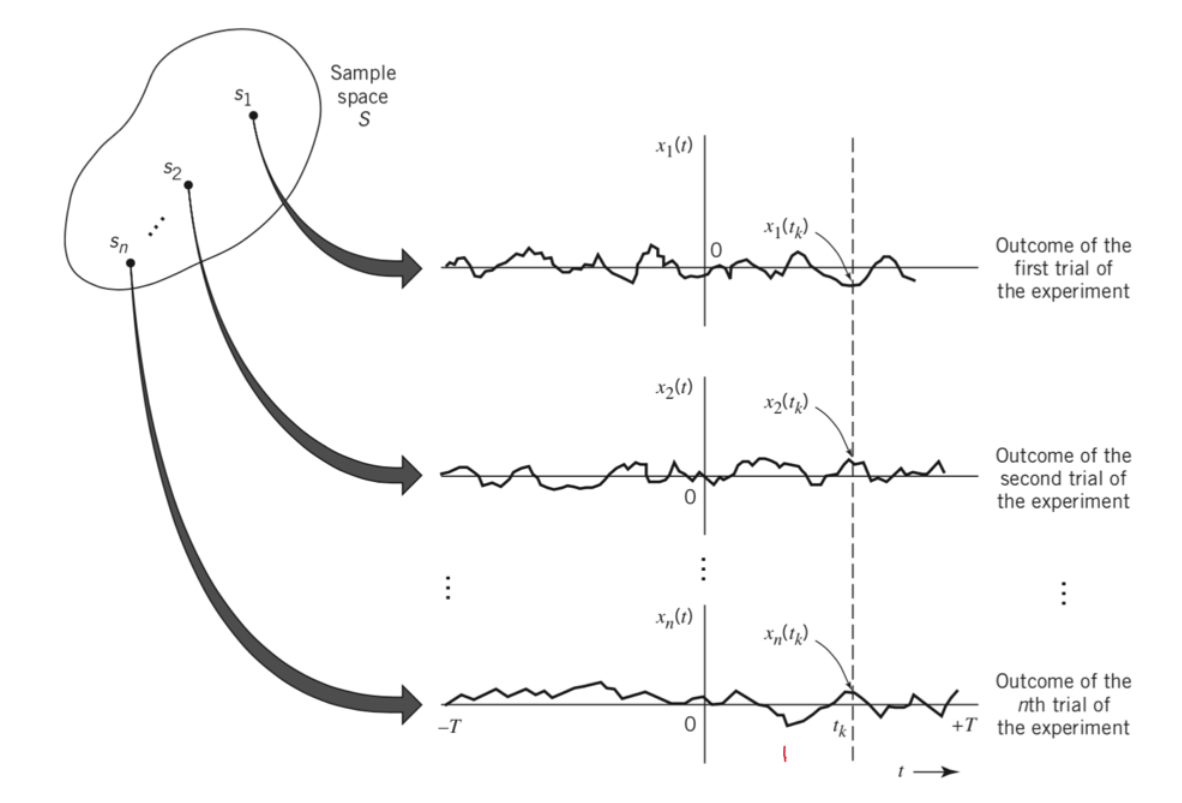
\includegraphics[width = 6cm]{media/processi stocastici.png}
        \end{figure}
        al campionamento $t_k$ ho un set di variabili aleatorie. L'aletorietá puó essere derivante da uno o piú fattori,
        ad esempio in una funzione cosinusoidale $Acos(2\pi f_ct+\Theta)$ possono essere aleatorie ampiezza, frequenza e fase.

    \subsection{Valore medio}
        Consideriamo un processo stocastico reale $X_{(t)}$, il valore medio é l'expectation della variabile aleatoria ottenuta campionando
        il processo al tempo $t$:
            \[
                \mu_{X(t)} = \mathbb{E}[X_{(t)}] = \int_{-\infty}^{\infty}xf_{X_{(t)}(t)}dt
            \]
        ad ogni istante di tempo $t$ ho una nuova variabile aleatoria per questo é funzione del tempo.
    \subsection{Autocorrelazione}
        Consideriamo un processo stocastico reale $X_{(t)}$ e due variabili aleatorie associate $X_{(t_1)}$ e $X_{(t_2)}$. 
        L'autocorrelazione é l'expectation del prodotto delle due variabili aleatorie:
        \[
            R_{XX(t_1,t_2)} = \mathbb{E}[X_{t_1}X_{t_2}] = \int_{-\infty}^{\infty}\int_{-\infty}^{\infty} x_1x_2f_{X_{(t_1)},X_{(t_2)}(x_1,x_2)}dx_1dx_2
        \]
        \subsubsection{Propietá della autocorrelazione $R_x$}
            \begin{itemize}
                \item {Paritá: $R_{X(\tau)} = R_{X(-\tau)}$}
                \item {$R_{X(0)}\geq \underset{Val.\ Massimo}{\underbrace{\left|R_{X(\tau)}\right|}}$: Cosa rappresenta?
                    \begin{align}
                        R_{X(\tau)} &= \mathbb{E}[X_{(t_1)}X_{(t_2)}]=\eval*{\mathbb{E}[X_{(t)}X_{(t-\tau)}] }_{\tau = 0} \nonumber \\
                        R_{X(0)}    &= \underset{Potenza}{\underbrace{\mathbb{E}[|X|^2]}} = \int_{-\infty}^{\infty} x^2f_{X_{(t)}(t)}dx \nonumber
                    \end{align}
                    coincide con la potenza del processo SSL.
                }
            \end{itemize}
        \subsubsection{Sigificato fisico dell'autocorrelazione}
            La funzione di autocorrelazione ci fornisce la possibilitá di descrivere l'indipendenza di due variabili aleatorie ottenute dal campionamento
            del processo stocastico $X_{(t)}$ a tempi divesti. Piú il processo stocastico $X_{(t)}$ cambia nel tempo, piú rapidamente la funzione di autocorrelazione 
            scenderá dal suo massimo $R_{XX(0)}$
            \begin{figure}[H]
                \centering
                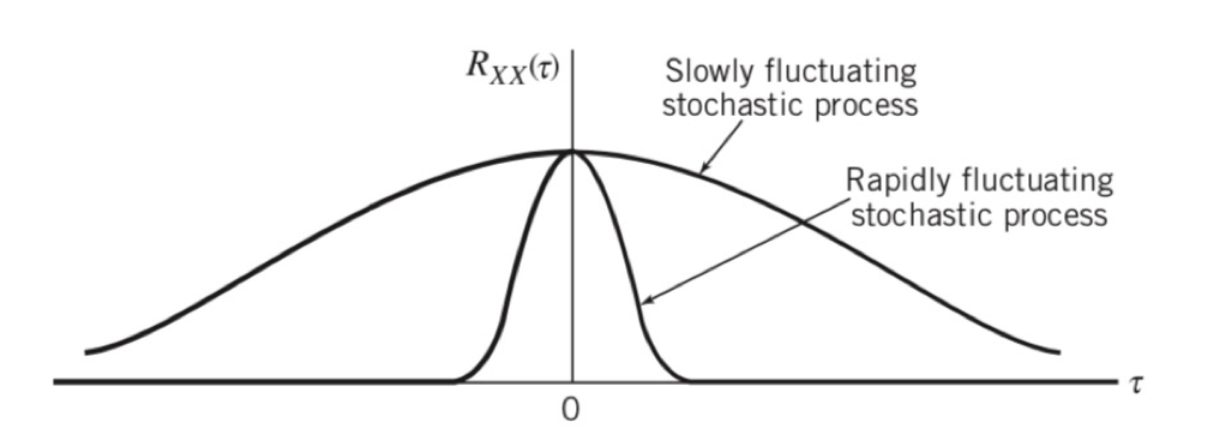
\includegraphics[width = 8cm]{media/autocorrelazione stocastica.png}
            \end{figure}
    \subsection{Sitemi Stazionari in Senso Lato (SSL)}\label{Sitemi Stazionari in Senso Lato (SSL)}
        Un processo stocastico $X_{(t)}$ si dice Stazionario in Senso Lato (SSL) se:
        \begin{itemize}
            \item {Il valore medio del processo $X_{(t)}$ é costante $\forall t$:
                \[
                    \mu_{X(t)} = \mathbb{E}[X_{(t)}] \overset{SSL}{\Rightarrow} \mu_{X}    
                \]
            }
            \item {La funzione di autocorrelazione del processo $X_{(t)}$ dipende solamente dalla differenza tra la differenza 
                tra due tempi qualsiasi al quale il processo é campionato:
                \[
                    R_{XX(t_1,t_2)} = \mathbb{E}[X_{(t_1)}X_{(t_2)}] \overset{SSL}{\Rightarrow} R_{X(t_1-t_2)} = R_{X(\tau)}      
                \]
                Se il processo dipende solo da $\tau$ posso farne la $TCF$ e analizzarne la densitá spettrale. 
                }
        \end{itemize} 
        \subsubsection{Trasmissione di un SSL in un sistema LTI-Filter}
            Supponiamo di avere un processo stocastico $X_{(t)}$ in ingresso ad un sistema LTI-Filter di risposta $h_{(t)}$,
            producendo un nuvo processo stocastico $Y_{(t)}$
            \begin{figure}[H]
                \centering
                \begin{tikzpicture}[
                        node distance=2cm,
                        >=latex
                    ]
                    % Blocks
                    \node [coordinate] (input) {};
                    \node [rectangle, draw,minimum height=3em, minimum width=3em,right of=input] (filter) {$LTI:\ h_{(t)}$};
                    \node [coordinate, right of=filter] (output) {$s_{(t)}$};
                
                    % Connections
                    \draw [->] (input) --node[above]{$X_{(t)}$} (filter);
                    \draw [->] (filter) --node[above]{$Y_{(t)}$} (output);
                \end{tikzpicture}    
            \end{figure}
            l'uscita $Y_{(t)}$ si calcola con la convoluzione:
            \[
                Y_{(t)} = X_{(t)} \otimes h_{(t)} = \int_{-\infty}^{\infty} X_{(\alpha)} h_{(t-\alpha)} d\alpha
            \]
            Calcoliamone gli indici:
            \begin{itemize}
                \item {
                    Valore medio:
                    \begin{align}
                        \mu_Y &= \mathbb{E}[Y_{(t)}] =\mathbb{E}[X_{(t)} \otimes h_{(t)}] = \mathbb{E}\left[\int_{-\infty}^{\infty} X_{(\alpha)} h_{(t-\alpha)} d\alpha\right]\nonumber \\
                              &\overset{\ref{linearita expectation}}{=} \int_{-\infty}^{\infty} \mathbb{E}[X_{(\alpha)}] h_{(t-\alpha)} d\alpha = \int_{-\infty}^{\infty} \mu_{X_{(\alpha)}} h_{(t-\alpha)} d\alpha  \nonumber \\
                              &=  \mu_{X_{(t)}} \otimes h_{(t)}\nonumber
                    \end{align}
                }
                \item {
                    Autocorrelazione:
                    \begin{align}
                        R_{YY(t_1,t_2)} &= \mathbb{E}[Y_{(t_1)}Y_{(t_2)}] = \mathbb{E}\left[\int_{-\infty}^{\infty} X_{(\alpha_1)} h_{(t-\alpha_1)} d\alpha_1\int_{-\infty}^{\infty} X_{(\alpha_2)} h_{(t-\alpha_2)} d\alpha_2\right]\nonumber \\
                                        &= \int_{-\infty}^{\infty}\int_{-\infty}^{\infty} \mathbb{E}[X_{(\alpha_1)}X_{(\alpha_2)}] h_{(t-\alpha_1)} h_{(t-\alpha_2)} d\alpha_1d\alpha_2\nonumber \\
                                        &\overset{C. Var.}{=} R_{X(t_1,t_2)} \otimes h_{(t_1)}\otimes h_{(t_2)}\nonumber
                    \end{align}
                }
            \end{itemize}
            Supponiamo adesso che il processo $X_{(t)}$ sia SSL, verifchiamo se anche $Y_{(t)}$ é SSL:
            \paragraph{Valore Medio:}
                \begin{align}
                    \mu_Y &= \mathbb{E}[Y_{(t)}] = \int_{-\infty}^{\infty} \mathbb{E}[X_{(\alpha)}] h_{(t-\alpha)} d\alpha = \int_{-\infty}^{\infty} \mu_{X_{(\alpha)}} h_{(t-\alpha)} d\alpha \nonumber \\
                            &= \mu_{X_{(\alpha)}} \int_{-\infty}^{\infty} h_{(t-\alpha)} d\alpha \overunderset{\beta = t-\alpha}{d\beta = -d\alpha}{=} \mu_{X_{(\alpha)}} \int_{-\infty}^{\infty} h_{(\beta)} d\beta\nonumber \\
                            &= \mu_X H_{(0)}\nonumber
                \end{align}
                si $H_{(0)}$ é proprio il grande ritorno di una $TCF$, viene fuori perché se calcoliamo la $TCF$ in $0$
                \[
                    \eval*{\int_{-\infty}^{\infty} h_{(\beta)} e^{-j2\pi f\beta} d\beta}_{f = 0} = \int_{-\infty}^{\infty} h_{(\beta)} d\beta = H_{(0)}
                \]
                il quale coincide con il valore medio.
            \paragraph{Autocorrelazione:}
                \begin{align}
                    R_{Y(t_1,t_2)} &= R_{X(\tau)}\otimes h_{(\tau)} \otimes h_{(-\tau)} \nonumber \\
                                    &= \int_{-\infty}^{\infty}\int_{-\infty}^{\infty} h_{(\tau_1)}h_{(\tau_2)} R_{XX(\tau+\tau_1-\tau_2)} d\tau_1d\tau_2\nonumber
                \end{align}    
        \subsubsection{Densitá di potenza spettrale}\label{Densita di potenza spettrale}
            Supponiamo di voler caratterizzare l'output di $Y_{(t)}$ usando il dominio della frequenza:
            \[
                \mathbb{E}[Y_{(t)}^2] = \int_{-\infty}^{\infty} \left|H_{(f)}\right|^2 S_{XX(f)} df  
            \]
            dove $S_{XX(f)}$ é la Densitá di potenza spettrale:
            \[
                S_{XX(f)} = \int_{-\infty}^{\infty} R_{XX(\tau)} e^{-j2\pi f\tau}d\tau
            \]
            ma perché menziona la potenza?
            \begin{align}
                P_x &= \mathbb{E}[X^2] = R_{X(0)} \overset{ATCF[S_{X(f)}]}{=} \eval*{\int_{-\infty}^{\infty} S_{X(f)} e^{j2\pi f\tau}df}_{\tau=0} \nonumber \\
                    &=  \int_{-\infty}^{\infty} S_{X(f)}df \nonumber
            \end{align}
            trovo la relazione per l'uscita $Y_{(t)}$:
            \begin{figure}[H]
                \centering
                \begin{tikzpicture}[
                        node distance=2cm,
                        >=latex
                    ]
                    % Blocks
                    \node [coordinate] (input) {};
                    \node [rectangle, draw,minimum height=3em, minimum width=3em,right of=input] (filter) {$LTI:\ h_{(t)}$};
                    \node [coordinate, right of=filter] (output) {$s_{(t)}$};
                
                    % Connections
                    \draw [->] (input) --node[above]{$X_{(t)}$} node[below]{$S_{X(t)}$} (filter);
                    \draw [->] (filter) --node[above]{$X_{(t)}$} node[below]{$S_{Y(t)}$} (output);
                \end{tikzpicture}    
            \end{figure}            
            \begin{align}
                S_{Y(f)} &= TCF[R_X] =TCF[ R_{X(\tau)}\otimes h_{(\tau)} \otimes h_{(-\tau)}] \overset{\ref{Conv. Distributiva}}{=}  S_{X(f)}H_{(f)} H_{(-f)}    \nonumber \\
                         &\overset{\ref{Simmetria Hermitiana}}{=} S_{X(f)}H_{(f)} H^\ast_{(f)} =  S_{X(f)}|H_{(f)}|^2\nonumber
            \end{align}
            trovo che la densitá spettrale di potenza di $Y_{(t)}$ é la densitá spettrale di potenza di $X_{(t)}$ per il modulo quadro della
            risposta del filtro e la sua misura é in watt per hertz ($W/Hz$).
    \subsection{Processo Gaussiano}
        Un processo $Y_{(t)}$ é detto processo Gaussiano se la variabile aleatoria $Y$ é una variabile aleatoria a distribuzione Gaussiana:
        \[
            f_{Y(y)} = \frac{1}{\sqrt{2\pi}\sigma}e^{\left(\displaystyle-\frac{(y-\mu)^2}{2\sigma^2}\right)}    
        \] 
        \paragraph{Propietá:}
        \begin{itemize}
            \item {
                Il processo stocastico creato da un fenomeno fisico solitamente é possibile ricondurlo a un modella Gaussiano.
            }
            \item {
                L'uso di un modello Gaussiano per un fenomeno fisico é spesso confermato dagli esperimenti.
            }
            \item {
                Il teorema del limite centrale (\ref{Teorema del Limite Centrale - Central Limit Theorem}) fornisce una giustificazione matematica per la 
                distribuzione Gaussiana.
            }
        \end{itemize}
        \subsubsection{Rumore Bianco}
            É una sorgente di rumore idealizzata in modo tale da rendere lo spettro di densitá di potenza costante ($\frac{N_0}{2}$), cioé indipendente
            dalla frequenza a cui operiamo. L'aggettivo "Bianco" deriva dall'ottica: un segnale di luce bianca contine in ugual maniera tutte le frequenze
             all'interno dello spettro visivo. Ne possiamo dare una definizione approssimativa:
             \begin{center}
                Il rumore bianco, identificato da $W_{(t)}$ é un processo stazionario con densitá di potenza spettrale $S_{W(f)}$ con valore
                costante in tutto l'intervallo delle frequenze:
                \[
                    S_{WW(f)} = \frac{N_0}{2}\ \forall f  
                \]
             \end{center}
             \begin{figure}[H]
                \centering
                \subfloat[Densitá di potenza spettrale]{
                    \begin{tikzpicture}
                        \begin{axis}[
                            xlabel=$f$,
                            ylabel=$S_{W(f)}$,
                            xmin=-4,
                            xmax=5,
                            ymin=-0.2,
                            ymax=2,
                            ytick = {1},
                            xtick={},
                            xticklabels={},
                            yticklabel style = {yshift=6pt,xshift=4pt}, 
                            yticklabels = {$\frac{N_0}{2}$},
                            axis lines=middle,
                            domain=-4:4,
                            samples=100,
                            width=6.5cm,
                            height=4cm
                        ]
                        \addplot [const plot, blue, thick] coordinates{(-4,1)(4,1)};
                        \end{axis}
                    \end{tikzpicture}
                }
                \hfill
                \subfloat[Autocorrelazione]{
                    \begin{tikzpicture}
                        \begin{axis}[
                            xlabel=$\tau$,
                            ylabel=$R_{X(\tau)}$,
                            xmin=-4,
                            xmax=5,
                            ymin=-0.2,
                            ymax=2,
                            ytick = {1},
                            xtick={},
                            xticklabels={},
                            yticklabel style = {yshift=5pt,xshift=4pt}, 
                            yticklabels = {$\frac{N_0}{2}\delta_{(\tau)}$},
                            axis lines=middle,
                            domain=-5:5,
                            samples=100,
                            width=6.5cm,
                            height=4cm
                        ]
                        \addplot+ [blue, thick,mark = triangle] coordinates{(0,0)(0,1)};
                        \end{axis}
                    \end{tikzpicture}
                }
            \end{figure}
            \paragraph{Propietá:}
            \begin{itemize}
                \item {Dato che $R_{W(\tau)}=0\ \forall \tau\neq 0$ ne segue che due differenti campionamenti del rumore bianco sono completamente
                incorrelati tra loro}
                \item {
                    Se il rumore bianco é Gaussiano allore due campioni sono statisticamente indipendenti.
                }
                \item {
                    Finché la banda di un processo del rumore in ingresso al sistema é ampiamente maggiore della banda del sistema stesso, allora possiamo modellare
                    il rumore come un processo a rumore bianco.
                }
            \end{itemize}
        \subsubsection{Filtro passa basso ideale per rumore bianco}
            Supponiamo di avere un ricevitore:
            \begin{figure}[H]
                \centering
                    \begin{tikzpicture}[
                            node distance=2cm,
                            >=latex
                        ]
                        % Blocks
                        \node [circle,draw] (RXant) {$r_{(t)}$};
                        \node [rectangle, draw,minimum height=1em, minimum width=2em,right of=RXant] (RX) {$RX$};
                        \node [rectangle, draw,minimum height=1em, minimum width=2em,right of=RX] (DC) {$LP_{(B)}$};
                        \node [rectangle, draw,minimum height=1em, minimum width=2em,right of=DC] (DS) {$kT$};
                        \node [coordinate,right of = DS] (output) {};
                    
                        % Connections
                        \draw [->] (RXant) --node[above]{} (RX);
                        \draw [->] (RX) --node[above]{$r_{(t)}$} (DC);
                        \draw [->] (DC) --node[above]{$x_{(t)}$} (DS);
                        \draw [-] (DS) --node[above]{$x_{[k]}$} (output);
                    \end{tikzpicture}    
            \end{figure}
            e un rumore additivo:
            \begin{figure}[H]
                \centering
                    \begin{tikzpicture}[
                            node distance=2.5cm,
                            >=latex
                        ]
                        % Blocks
                        \node [circle,draw] (TXant) {$s_{(t)}$};
                        \node [circle, draw,right of=TXant] (sum) {$+$};
                        \node [rectangle, draw,below of = sum,minimum height=1em, minimum width=2em] (error) {$n_{(t)}$};
                        \node [circle,draw,right of=sum] (RXant) {$r_{(t)}$};
                    
                        % Connections
                        \draw [->] (TXant) --node[above]{$s_{(t)}$} (sum);
                        \draw [->] (sum) --node[above]{$\scriptstyle r_{(t)} = s_{(t)}+ n_{(t)}$} (RXant);
                        \draw [->] (error) -- (sum);
                    \end{tikzpicture}    
            \end{figure}
            inviamo un segnale $s_{(t)}$ con banda $B$:
            \begin{figure}[H]
                \centering
                \subfloat[Trasmettitore]{
                    \begin{tikzpicture}
                        \begin{axis}[
                            xlabel=$f$,
                            ylabel=$S_{W(f)}$,
                            xmin=-5,
                            xmax=5,
                            ymin=-0.2,
                            ymax=1,
                            ytick = {1},
                            xtick={-2,2},
                            xticklabels={$-B$,$B$},
                            yticklabel style = {yshift=6pt,xshift=4pt}, 
                            yticklabels = {$\frac{N_0}{2}$},
                            axis lines=middle,
                            domain=-5:5,
                            samples=800,
                            width=6.5cm,
                            height=4cm
                        ]
                        \addplot [const plot, blue, thick, domain = -2:2] {gauss(0,0.8)-0.01};
                        \end{axis}
                    \end{tikzpicture}
                }
                \hfill
                \subfloat[Ricevitore: ${\color{blue}s_{(t)}}+ {\color{purple}n_{(t)}}$]{
                    \begin{tikzpicture}
                        \begin{axis}[
                            xlabel=$\tau$,
                            ylabel=$R_{X(\tau)}$,
                            xmin=-5,
                            xmax=5,
                            ymin=-0.2,
                            ymax=1,
                            ytick = {1},
                            xtick={-2,2},
                            xticklabels={$-B$,$B$},
                            yticklabel style = {yshift=5pt,xshift=4pt}, 
                            yticklabels = {$\frac{N_0}{2}\delta_{(\tau)}$},
                            axis lines=middle,
                            domain=-5:5,
                            samples=800,
                            width=6.5cm,
                            height=4cm
                        ]
                        \addplot [const plot, blue, thick, domain = -2:2] {gauss(0,0.8)-0.01};
                        \addplot [const plot, purple, thick] coordinates{(-5,0.2)(5,0.2)};
                    \end{axis}
                    \end{tikzpicture}
                }
                \
            \end{figure}
            il ricevitore si occupa adesso del filtraggio con un filtro passa basso di banda $B$ ($LP_{(B)}$), ritrovando il 
            segnale originale ma con il rumore additivo:
            \begin{figure}[H]
                \centering
                \begin{tikzpicture}
                    \begin{axis}[
                        xlabel=$\tau$,
                        ylabel=$R_{X(\tau)}$,
                        xmin=-5,
                        xmax=5,
                        ymin=-0.2,
                        ymax=1,
                        ytick = {0.6},
                        xtick={-2,2},
                        xticklabels={$-B$,$B$},
                        yticklabel style = {yshift=5pt,xshift=4pt}, 
                        yticklabels = {$1$},
                        axis lines=middle,
                        domain=-5:5,
                        samples=800,
                        width=8cm,
                        height=5cm
                    ]
                    \addplot [const plot, blue, thick, domain = -2:2] {gauss(0,0.8)-0.01};
                    \addplot [const plot, purple, thick] coordinates{(-5,0.2)(5,0.2)};
                    \addplot [const plot, orange, thick] coordinates{(-5,0)(-2,0)(-2,0.6)(2,0.6)(2,0)(5,0)};
                \end{axis}
                \end{tikzpicture}
                \caption{${\color{blue}s_{(t)}},{\color{purple}n_{(t)}},{\color{orange}LP-filter}$}
            \end{figure}
            in uscita dal filtro ho $x_{(t)} = s_{(t)} + n_{(t)} \otimes h_{(t)}$ con la densitá spettrale del rumore:
            \[
                S_{W(f)} = S_{n(f)} |H_{(f)}|^2 = S_{n(f)} 
            \]
            Per ricostruire il segnale devo campionare con una $f_s = \frac{1}{T_s} = 2B$ ($kT$):
            \[
                x_{[k]} = x_{(t=kT)} = s_{[k]}+w_{[k]}    
            \]
            Cosa succede al rumore?
            Nel dominio della frequenza lo spettro di rumore filtrato,$w_{[k]}$, é  una somma di delta di dirac ho quindi $S_{w(f)} = rect\left(\frac{f}{2B}\right)$
            trasformadola nel dominio del tempo, cioé calcolando la sua autocorrelazione per $ATCF[S_{w(f)}] = R_{w(\tau)}$ ottengo $R_{w(\tau)} = 2B\tau sinc(2B\tau)$,
            campionandola rispetto alla banda del filtro $B$ in $\frac{k}{2B}$ la $sinc$ é sempre $0$ rendendo le variabili del rumore Gaussiano statisticamente 
            indipendenti a valore medio nullo e varianza $N_0B$. 
            \[
                \eval*{R_{w(\tau)}}_{\tau=kT} =\eval*{\mathbb{E}[w_{(t)}w_{(t-\tau)}]}_{\tau=kT} \overset{T=\frac{1}{2B}}{=} 0  
            \]
            \begin{figure}[H]
                \centering
                \begin{tikzpicture}
                    \begin{axis}[
                        xlabel=$\tau$,
                        ylabel=$R_{X(\tau)}$,
                        xmin=-5,
                        xmax=5,
                        ymin=-1,
                        ymax=1.5,
                        ytick={1},
                        yticklabels = {$N_0B$},
                        yticklabel style = {yshift=5pt,xshift=4pt}, 
                        xtick={-4,-3,-2,-1,1,2,3,4},
                        xticklabels={$-\frac{4}{2B}$,$-\frac{3}{2B}$,$-\frac{2}{2B}$,$-\frac{1}{2B}$,$\frac{1}{2B}$,$\frac{2}{2B}$,$\frac{3}{2B}$,$\frac{4}{2B}$},
                        xticklabel style = {yshift=-3pt}, 
                        axis lines=middle,
                        domain=-5:5,
                        samples=800,
                        width=10cm,
                        height=6cm
                    ]
                    \addplot [blue, thick, samples = 800] {sin(deg(x*pi))/(x*pi)};
                \end{axis}
                \end{tikzpicture}
            \end{figure}
            per questo il modello $Y = S + n \sim \mathcal{N} (0,\sigma^2)$ é giusto per approssimare il rumore. Calcoliamone il valor medio e varianza:
            \begin{gather}
                w_{(t)} \sim \mathcal{N}(0,\sigma^2_w)  \nonumber \\
                \sigma^2_w = \mathbb{E}[X^2]-\mu_w = \mathbb{E}[X^2] = R_{w(0)} = N_0B\nonumber
            \end{gather}
            Ne segue che piú la banda é elevata piú rumore entra nel sistema.            







    \section{Sistemi di Comunicazione}
    Un sistema di comunicazione numerico puó essere approssimato a
    \begin{figure}[H]
        \centering 
        \begin{tikzpicture}[
            node distance=3cm,
            >=latex
            ]

            \node [coordinate] (input) {};
            \node [draw, rectangle,right of = input, minimum height=3em, minimum width=6em] (block) {$\substack{\text{Sistema di} \\ \text{Comunicazione Numerico}}$};
            \node [coordinate, right of = block] (output) {};
            
            \draw[draw,->] (input) --node[above]{$\{b_n$\}} (block);
            \draw[->] (block) --node[above]{$\{\hat{b}_n$\}} (output);
        \end{tikzpicture}    
    \label{sistema di comunicazione numerico}
    \end{figure}
    Dove all'interno del sistema sono racchiusi il Trasmettitore ($Tx$), il canale di trasmissione ($c$) e il Ricevitore ($Rx$).
    il sistema prende in ingresso dei bit, o un segnale analogico opportunamente numerizzato, e li trasmette su di un canale numerico inviandoli ad un ricevitore.
    Analizziamo la parte di trasmissione:
    \begin{figure}[H]
        \centering
            \begin{tikzpicture}[
                    node distance=2cm,
                    >=latex
                ]
                % Blocks
                \node [coordinate] (input) {};
                \node [rectangle, draw,minimum height=1em, minimum width=2em,right of=input] (AD) {$kT$};
                \node [rectangle, draw,minimum height=1em, minimum width=2em,right of=AD] (Q) {$Q$};
                \node [rectangle, draw,minimum height=1em, minimum width=2em,right of=Q] (CS) {$CdC$};
                \node [rectangle, draw,minimum height=1em, minimum width=2em,right of=CS] (CC) {$Map$};
                \node [rectangle, draw,minimum height=1em, minimum width=2em,right of=CC] (TX) {$Mod$};
                \node [circle,draw,right of=TX] (TXant) {$s_{T(t)}$};
            
                % Connections
                \draw [->] (input) --node[above]{\scriptsize$x_{(t)}$} (AD);
                \draw [->] (AD) --node[above]{\scriptsize$x_{[kT]}$} (Q);
                \draw [->] (Q) --node[above]{\tiny$\{b_n\}$}node[midway]{\tiny$/$} node[below]{\scriptsize$k$} (CS);
                \draw [->] (CS) --node[above]{\tiny$\{d_n\}$}node[midway]{\tiny$/$} node[below]{\scriptsize$n$} (CC);
                \draw [->] (CC) --node[above]{\tiny$\{a_i\}$} (TX);
                \draw [-] (TX) -- (TXant);
            \end{tikzpicture}    
        \label{fig:Sistema di comunicazione numerico trasmettitore}
        \caption{Esempio sistema di trasmettitore}
    \end{figure}
    \begin{itemize}
        \item {CdC: Codifica di Canale, si occupa di aggiungere ridondanza ai bit in ingresso per proteggerli da eventuali errori del canale di trasmissione ho di
            conseguenza che $k<n$, puó essere preceduto da un eventuale codifica di sorgente. 
            \begin{figure}[H]
                \centering 
                \begin{tikzpicture}[
                    node distance=3cm,
                    >=latex
                    ]
        
                    \node [coordinate] (input) {};
                    \node [draw, rectangle,right of = input, minimum height=3em, minimum width=6em] (block) {$\substack{\text{Codifica di} \\ \text{Canale}}$};
                    \node [coordinate, right of = block] (output) {};
                    
                    \draw[draw,->] (input) --node[above]{$\{b_n$\}} node[midway]{\tiny$/$} node[below]{\scriptsize$k,R_b$}(block);
                    \draw[->] (block) --node[above]{$\{d_n$\}} node[midway]{\tiny$/$} node[below]{\scriptsize$n,R_d$} (output);
                \end{tikzpicture}    
            \end{figure}
            $R_b = \frac{1}{T_b}$ é il Bit Rate a cui i bit sono generati in ingresso mentre, $R_d = \frac{1}{T_d}$ é il Bit Rate di uscita. Volendo trovare la relazione tra ingresso e uscita:
            \[
                kT_b = nT_d \Rightarrow \frac{R_b}{R_d} = \frac{k}{n}     
            \] 
            il quale é compreso tra $0<\frac{R_b}{R_d}\leq 1$ se cosí non fosse non introdurrei ridondanza, il rate in ingresso deve essere inferiore a quello di uscita o non 
            potrei introdurre bit aggiuntivi.
        }
        \item {Map: Mappatore ($M$), trasforma una \emph{sequenza} di bit di codice $\{d_n\}$ in una sequenza di simboli $\{a_i\}$ appartenenti ad un alfabeto $A$ costituito
            da $M$ diversi simboli, dove $M$ é tipicamente una potenza del $2$. Ponendo $M=2^q$ il mappatore associa un simbolo di modulazione a ciascun blocco di $Q$ bit di canale. 
            \begin{figure}[H]
                \centering 
                \begin{tikzpicture}[
                    node distance=3cm,
                    >=latex
                    ]
        
                    \node [coordinate] (input) {};
                    \node [draw, rectangle,right of = input, minimum height=3em, minimum width=6em] (block) {Mappatore};
                    \node [coordinate, right of = block] (output) {};
                    
                    \draw[draw,->] (input) --node[above]{$\{d_n$\}} node[below]{$R_d$} (block);
                    \draw[->] (block) --node[above]{$\{a_i$\}} node[below]{$f_s$} (output);
                \end{tikzpicture}    
            \end{figure}
            Ad esempio una mappa quaternaria:
            \begin{table}[H]
                \centering
                \begin{tabular}{c|c}
                $\{d_n\}$  & $\{a_i\}$ \\ \hline
                {00} & {-3}     \\
                {01} & {-1}     \\
                {10} & {1}     \\
                {11} & {3}    
                \end{tabular}
            \end{table}
            \begin{figure}[H]
                \centering
                \subfloat{
                    \begin{tikzpicture}
                        \begin{axis}[
                            xlabel=$t$,
                            ylabel=$d_n$,
                            xmin=-0.1,
                            xmax=5,
                            ymin=-0.2,
                            ymax=1,
                            ytick = {0,0.5},
                            xtick={0.5,1.5,2.5,3.5,4.5},
                            xticklabels={$1$,$0$,$1$,$1$},
                            % yticklabel style = {yshift=6pt,xshift=4pt}, 
                            yticklabels = {$0$,$1$},
                            axis lines=middle,
                            domain=-0.1:5,
                            samples=800,
                            width=6.5cm,
                            height=5cm
                        ]
                        \addplot [const plot, blue, thick] coordinates{(0,0.5)(1,0.5)(1,0)(2,0)(2,0.5)(4,0.5)(4,0)};
                        \addplot [const plot, dotted, blue] coordinates{(3,0)(3,0.5)};
                        \end{axis}
                    \end{tikzpicture}
                }
                \hfill
                \subfloat{
                    \begin{tikzpicture}
                        \begin{axis}[
                            xlabel=$t$,
                            ylabel=$a_i$,
                            xmin=-0.1,
                            xmax=5,
                            ymin=-1.5,
                            ymax=1.5,
                            ytick = {-1,-0.5,0.5,1},
                            yticklabels = {$-3$,$-1$,$1$,$3$,},
                            xtick={1,2},
                            xticklabels={$10$,$11$},
                            % yticklabel style = {yshift=6pt,xshift=4pt}, 
                            axis lines=middle,
                            domain=-0.1:5,
                            samples=800,
                            width=6.5cm,
                            height=6cm
                        ]
                        \addplot [const plot, blue, thick] coordinates{(0,0.5)(2,0.5)(2,1)(4,1)(4,-0.5)};
                    \end{axis}
                    \end{tikzpicture}
                }
            \end{figure}
            il periodo $T$ tra due \emph{simboli} adiacenti viene detto "Intervallo di Segnalazione". Se $M=2^q$ allora:
            \[
                T = qT_d =T_d log_{2}(M)  
            \]
            la velocitá di trasmissione dei simboli $f_s = \frac{1}{T}$ é legata al rate $R_d$ da:
            \[
                f_s = \frac{R_d}{Q} = \frac{R_d}{log_{2}(M)} 
            \] 
            devo caricare velocemente i simboli in ingresso al mappatore per poter completare la sequenza da mappare. Si nota anche come
            all'aumentare della cardinalitá $M$ la velocitá diminuisca, la sua misura é fatta in $BAUD = \frac{simboli}{sec}$
        }
        \item {Mod: Modulatore converte la sequenza dei simboli $\{a_i\}$ in un segnale analogico $s_{T(t)}$ in modo tale da poter essere trasmesso  
            sul canale di comunicazione. Puó essere una modulazione {\color{blue}BB} o {\color{red}BP}, in ogni caso la banda impiegata sará:
            \[
                B_T \simeq \frac{1}{T}  
            \]
            volendolo esprimere in relazione ai vari bit rate:
            \[
                B_T = \frac{1}{T} \overset{T = qT_d}{=} \frac{1}{qT_d} = \frac{1}{T_d log_2(M)} = \frac{nR_b}{klog_2(M)}     
            \]
            osserviamo come aumentando la cardinalitá $M$ della mappa riduco la banda, ció é molto utile per poter occupare uno spettro limitato ma ridurla troppo
            comporta un aumento dell'errore. Invece un rate del codice $\frac{n}{k}$ influenza sia la banda occupata che l'errore dei simboli, si tendono 
            a usare codici che abbiano un rate vicino all'$1$. 
        }
    \end{itemize}
    Analizziamo la parte del ricevitore:
    \begin{figure}[H]
        \centering
            \begin{tikzpicture}[
                    node distance=3cm,
                    >=latex
                ]
                % Blocks
                \node [circle,draw] (RXant) {$r_{(t)}$};
                \node [rectangle, draw,minimum height=2em, minimum width=2em,right of=RXant] (RX) {$\substack{\text{Demodulatore}\\\text{Numerico}}$};
                \node [rectangle, draw,minimum height=2em, minimum width=2em,right of=RX] (DC) {Demappatore};
                \node [rectangle, draw,minimum height=2em, minimum width=2em,right of=DC] (DS) {$\substack{\text{Decodifica di}\\\text{canale}}$};
                \node [coordinate,right of = DS] (output) {};
            
                % Connections
                \draw [->] (RXant) --node[above]{} (RX);
                \draw [->] (RX) --node[above]{$\{\hat{a}_i\}$} (DC);
                \draw [->] (DC) --node[above]{$\{\hat{d}_n\}$} (DS);
                \draw [->] (DS) --node[above]{$\{\hat{b}_n\}$} (output);
            \end{tikzpicture}    
        \caption{Esempio sistema ricevitore}
    \end{figure}
    Il segnale ricevuto $r_{(t)}$ viene demodulato dal demodulatore numerico, il quale ha il compito di fornire una stima dei simboli $\{\hat{a}_i\}$ trasmessi.
    In seguito vengono demappati in modo da ottenere una stima di $\{\hat{d}_n\}$ dei bit di codice. Infine passano nel decodificatore di canale la quale uscita 
    fornisce ua stima dei $\{\hat{b}_n\}$ bit di informazione.

    I vantaggi di un sistema di comunicazione numerico rispetto ad uno analogico sono:
    \begin{itemize}
        \item {
            Una maggiore resistenza al rumore, dovuta all'alfabeto dei simboli limitato, che consente di prendere decisioni affidabili.
        }
        \item {
            La possibilitá di utilizzare ripetizioni rigenerative anziché ripetizioni che amplificano semplicemente il segnale ricevuto, amplificando quindi sia il segnale
            utile che il rumore. 
        }
        \item {
            La possibilitá di utilizzare codici a correzione d'errore inserendo ridondanza nella sequenza di bit informativi.
        }
    \end{itemize}
    \subsection{Phase Amplitude Modulation - PAM}
        É una tipologia di sistema di comunicazione in {\color{blue}Banda Base}, il cui segnale trasmesso $s_{T(t)}$ ha densitá spettrale
        di potenza centrata in $0$. Il sistema PAM riceve in ingresso simboli di modulazione $\{a_i\}$ provenienti dal mappaggio dei bit $\{d_n\}$ 
        \subsubsection{Mappatore}
            Il mappatore ha come cardinalitá una potenza del $2$, abbiamo PAM con mappatura: binaria, quaternaria o ottale
            \begin{table}[H]
                \centering
                \subfloat[Mappa Binaria]{
                    \begin{tabular}{c|c}
                        $\{d_n\}$  & $\{a_i\}$ \\ \hline
                        {0} & {-1}     \\
                        {1} & {+1}     \\
                    \end{tabular}
                }
                \hfill
                \subfloat[Mappa Quaternaria]{
                    \begin{tabular}{c|c}
                        $\{d_n\}$  & $\{a_i\}$ \\ \hline
                        {00} & {-3}     \\
                        {01} & {-1}     \\
                        {10} & {+1}     \\
                        {11} & {+3}    
                    \end{tabular}
                }
                \hfill
                \subfloat[Mappa Ottale]{
                    \begin{tabular}{c|c}
                        $\{d_n\}$  & $\{a_i\}$ \\ \hline
                        {000} & {-7}\\
                        {001} & {-5}\\
                        {010} & {-3}\\
                        {011} & {-1}\\
                        {100} & {+1}\\
                        {101} & {+3}\\
                        {110} & {+5}\\
                        {111} & {+7}    
                    \end{tabular}
                }
            \end{table}
            \begin{figure}[H]
                \centering
                    \begin{tikzpicture}[
                            node distance=3cm,
                            >=latex
                        ]
                        % Blocks
                        \node [coordinate,draw] (RX) {};
                        \node [rectangle, draw,minimum height=3em, minimum width=2em,right of=RX] (DC) {$\substack{\text{Mappatore}\\\text{PAM}}$};
                        \node [rectangle, draw,minimum height=3em, minimum width=2em,right of=DC] (DS) {$\substack{\text{Modulatore}\\\text{PAM}}$};
                        \node [coordinate,right of = DS] (output) {};
                    
                        % Connections
                        \draw [->] (RX) --node[above]{$\{d_n\}$}node[below]{$R_d$} (DC);
                        \draw [->] (DC) --node[above]{$\{a_i\}$}node[below]{$f_s$} (DS);
                        \draw [->] (DS) --node[above]{$s_{T(t)}$} (output);
                    \end{tikzpicture}    
                \caption{Sistema PAM}
            \end{figure}
        \subsubsection{Modulatore}
            Il segnale PAM é una serie di impulsi che si susseguono in successione con un intervallo $T = \frac{1}{f_s}$ e modulatori in ampiezza dei simboli 
            $\{a_i\}$. Possiamo usare un qualsiasi impulso, che chiamiamo $g_{T(t)}$, basta che sia di durata finita:
            \begin{figure}[H]
                \centering
                \subfloat{
                    \begin{tikzpicture}
                        \begin{axis}[
                            xlabel=$t$,
                            ylabel=$g_{T(t)}$,
                            xmin=-0.1,
                            xmax=3,
                            ymin=-0.2,
                            ymax=1.5,
                            ytick = {1},
                            yticklabels = {$1$},
                            xtick={1},
                            xticklabels={$T$},
                            % yticklabel style = {yshift=6pt,xshift=4pt}, 
                            axis lines=middle,
                            domain=-0.1:3,
                            samples=800,
                            width=6.5cm,
                            height=5cm
                        ]
                        \addplot [const plot, blue, thick] coordinates{(0,1)(1,1)(1,0)};
                        \end{axis}
                    \end{tikzpicture}
                }
                \hfill
                \subfloat{
                    \begin{tikzpicture}
                        \begin{axis}[
                            xlabel=$t$,
                            ylabel=$g_{T(t)}$,
                            xmin=-0.1,
                            xmax=3,
                            ymin=-0.2,
                            ymax=1.5,
                            ytick = {1},
                            yticklabels = {$1$},
                            xtick={1},
                            xticklabels={$T$},
                            % yticklabel style = {yshift=6pt,xshift=4pt}, 
                            axis lines=middle,
                            domain=-0.1:3,
                            samples=800,
                            width=6.5cm,
                            height=5cm
                        ]
                        \addplot [const plot, blue, thick, domain = 0:1] {gauss(0.5,0.3)-0.35};
                        % \addplot [const plot, blue, thick,domain=0:1,samples = 500] {gauss(0.5,1)};
                    \end{axis}
                    \end{tikzpicture}
                }
            \end{figure}
            se il segnale non fosse di durata finita $T$ avrei sovrapposizione dei segnali (un po come nella $TDF$ \ref{Teorema del Campionamento - Nyquist Shannon} se campiono male), il modulatore calcola ad ogni istante il segnale
            \[
                s_{T(t)} = \sum_{i}a_ig_{T(t-iT)}  
            \]
            nello schema a blocchi si riduce a
            \begin{figure}[H]
                \centering
                    \begin{tikzpicture}[
                            node distance=3cm,
                            >=latex
                        ]
                        % Blocks
                        \node [coordinate,draw] (RX) {};
                        \node [rectangle, draw,minimum height=3em, minimum width=4em,right of=RX] (DC) {$g_{T(t)}$};
                        \node [coordinate,right of = DC] (output) {};
                    
                        % Connections
                        \draw [->] (RX) --node[above]{$\{a_i\}$} (DC);
                        \draw [->] (DC) --node[above]{$s_{T(t)}$} (output);
                    \end{tikzpicture}    
                \caption{Modulatore PAM}
            \end{figure}
            ne possiamo fare un esempio con una sequenza di simboli $\{a_i\} = \{+1,+3,-1,+1,-3\}$ e un impulso $g_{T(t)}$ del secondo tipo:
            \begin{figure}[H]
                \centering
                \subfloat[$\{a_i\}$]{
                    \begin{tikzpicture}
                        \begin{axis}[
                            xlabel=$t$,
                            ylabel=$\{a_i\}$,
                            xmin=-0.1,
                            xmax=5,
                            ymin=-0.2,
                            ymax=2.5,
                            ytick = {1},
                            yticklabels = {$1$},
                            xtick={1,2,3,4,5},
                            xticklabels={$T$,$2T$,$3T$,$4T$,$5T$},
                            % yticklabel style = {yshift=6pt,xshift=4pt}, 
                            axis lines=middle,
                            domain=-0.1:5,
                            samples=800,
                            width=10cm,
                            height=5cm
                        ]
                        \addplot [const plot, blue, thick] coordinates{(0,1)(1,1)(1,0)(1,1)(2,1)(2,0)(2,1)(3,1)(3,0)(3,1)(4,1)(4,0)(4,1)(5,1)(5,0)};
                        \node [] at (0.5,0.5) {$+1$};
                        \node [] at (1.5,0.5) {$+3$};
                        \node [] at (2.5,0.5) {$-1$};
                        \node [] at (3.5,0.5) {$+1$};
                        \node [] at (4.5,0.5) {$-3$};
                        \end{axis}
                    \end{tikzpicture}
                }
                \hfill
                \subfloat[$s_{T(t)}$]{
                    \begin{tikzpicture}
                        \begin{axis}[
                            xlabel=$t$,
                            ylabel=$s_{T(t)}$,
                            xmin=-0.1,
                            xmax=5,
                            ymin=-5,
                            ymax=5,
                            ytick = {1},
                            yticklabels = {$1$},
                            xtick={1,2,3,4,5},
                            xticklabels={$T$,$2T$,$3T$,$4T$,$5T$},
                            % yticklabel style = {yshift=6pt,xshift=4pt}, 
                            axis lines=middle,
                            domain=-0.1:5,
                            samples=800,
                            width=10cm,
                            height=8cm
                        ]
                        \addplot [const plot, orange, thick, domain = 0:1] {gauss(0.5,0.3)-0.34};
                        \addplot [const plot, orange, thick, domain = 1:2] {3*(gauss(1.5,0.3)-0.34)};
                        \addplot [const plot, orange, thick, domain = 2:3] {-gauss(2.5,0.3)+0.34};
                        \addplot [const plot, orange, thick, domain = 3:4] {gauss(3.5,0.3)-0.34};
                        \addplot [const plot, orange, thick, domain = 4:5] {-3*(gauss(4.5,0.3)-0.34)};
                        \addplot [const plot, dotted, thick] coordinates{(1,0)(1,5)};
                        \addplot [const plot, dotted, thick] coordinates{(2,0)(2,5)};
                        \addplot [const plot, dotted, thick] coordinates{(3,0)(3,5)};
                        \addplot [const plot, dotted, thick] coordinates{(4,0)(4,5)};
                        \addplot [const plot, dotted, thick] coordinates{(5,0)(5,5)};
                        \node [] at (0.5,3.5) {\small$a_0g_{T(t)}$};
                        \node [] at (1.5,3.5) {\small$a_1g_{T(t-T)}$};
                        \node [] at (2.5,3.5) {\small$a_2g_{T(t-2T)}$};
                        \node [] at (3.5,3.5) {\small$a_3g_{T(t-3T)}$};
                        \node [] at (4.5,3.5) {\small$a_4g_{T(t-4T)}$};

                        % \addplot [const plot, blue, thick,domain=0:1,samples = 500] {gauss(0.5,1)};
                    \end{axis}
                    \end{tikzpicture}
                }
            \end{figure}
            se invece utilizzassimo delle funzioni $g_{T(t)}$ rettangolari il segnale in uscita diventerebbe
            \begin{figure}[H]
                \centering
                \subfloat[$\{a_i\}$]{
                    \begin{tikzpicture}
                        \begin{axis}[
                            xlabel=$t$,
                            ylabel=$\{a_i\}$,
                            xmin=-0.1,
                            xmax=5,
                            ymin=-0.2,
                            ymax=2.5,
                            ytick = {1},
                            yticklabels = {$1$},
                            xtick={1,2,3,4,5},
                            xticklabels={$T$,$2T$,$3T$,$4T$,$5T$},
                            % yticklabel style = {yshift=6pt,xshift=4pt}, 
                            axis lines=middle,
                            domain=-0.1:5,
                            samples=800,
                            width=10cm,
                            height=5cm
                        ]
                        \addplot [const plot, blue, thick] coordinates{(0,1)(1,1)(1,0)(1,1)(2,1)(2,0)(2,1)(3,1)(3,0)(3,1)(4,1)(4,0)(4,1)(5,1)(5,0)};
                        \node [] at (0.5,0.5) {$+1$};
                        \node [] at (1.5,0.5) {$+3$};
                        \node [] at (2.5,0.5) {$-1$};
                        \node [] at (3.5,0.5) {$+1$};
                        \node [] at (4.5,0.5) {$-3$};
                        \end{axis}
                    \end{tikzpicture}
                }
                \hfill
                \subfloat[$s_{T(t)}$]{
                    \begin{tikzpicture}
                        \begin{axis}[
                            xlabel=$t$,
                            ylabel=$s_{T(t)}$,
                            xmin=-0.1,
                            xmax=5,
                            ymin=-5,
                            ymax=5,
                            ytick = {1},
                            yticklabels = {$1$},
                            xtick={1,2,3,4,5},
                            xticklabels={$T$,$2T$,$3T$,$4T$,$5T$},
                            % yticklabel style = {yshift=6pt,xshift=4pt}, 
                            axis lines=middle,
                            domain=-0.1:5,
                            samples=800,
                            width=10cm,
                            height=8cm
                        ]
                        \addplot [const plot, orange, thick] coordinates{(0,1)(1,1)(1,0)(1,3)(2,3)(2,0)(2,-1)(3,-1)(3,0)(3,1)(4,1)(4,0)(4,-3)(5,-3)(5,0)};
                        \addplot [const plot, dotted, thick] coordinates{(1,0)(1,5)};
                        \addplot [const plot, dotted, thick] coordinates{(2,0)(2,5)};
                        \addplot [const plot, dotted, thick] coordinates{(3,0)(3,5)};
                        \addplot [const plot, dotted, thick] coordinates{(4,0)(4,5)};
                        \addplot [const plot, dotted, thick] coordinates{(5,0)(5,5)};
                        \node [] at (0.5,3.5) {\small$a_0g_{T(t)}$};
                        \node [] at (1.5,3.5) {\small$a_1g_{T(t-T)}$};
                        \node [] at (2.5,3.5) {\small$a_2g_{T(t-2T)}$};
                        \node [] at (3.5,3.5) {\small$a_3g_{T(t-3T)}$};
                        \node [] at (4.5,3.5) {\small$a_4g_{T(t-4T)}$};

                        % \addplot [const plot, blue, thick,domain=0:1,samples = 500] {gauss(0.5,1)};
                    \end{axis}
                    \end{tikzpicture}
                }
            \end{figure}
            dovendo analizzare il dominio frequnziale di $s_{T(t)}$ sarebbero tutte delle $sinc$ in {\color{blue}BB}  
        \subsubsection{Densitá spettrale di potenza}\label{Densita spettrale di potenza - PAM}
            Volendo analizzare la banda del segnale in uscita al modulatore PAM potremmo pensare di utilizzare la $TCF$:
            \begin{gather}
                s_{T(t)} \overset{TCF\ref{TCF di segnali periodici}}{\rightleftharpoons} S_{T(f)}\nonumber\\
                s_{T(t)}  = \sum_{i}a_i g_{T(t-iT)} \overset{TCF\ref{TCF di segnali periodici}}{\rightleftharpoons} \sum_{i}a_i G_{T(f)} e^{-j2\pi fiT}  \nonumber
            \end{gather}
            ma non posso analizzare con la $TCF$ le variabili aleatorie $a_i$. Posso allora calcolare la Densitá spettrale di potenza (\ref{Densita di potenza spettrale}).
            Ammettiamo che la sequenza di simboli di modulazione $\{a_i\}$ sia SSL \ref{Sitemi Stazionari in Senso Lato (SSL)}. La sua media é
            \[
                \mu_a = \eta_a = \mathbb{E}[a_i]
            \]  
            e la sua funzione di autocorrelazione
            \[
                R_{a(m)} = \mathbb{E}[a_ia_{i+m}]    
            \]
            ho la densitá spettrale di potenza come 
            \begin{gather}
                S_{s(f)} = \frac{1}{T} S_{a(f)}\left|G_{T(f)}\right|^2 \nonumber \\
                S_{a(f)} = \sum_{m} R_{a(m)}e^{-j2\pi fmT} \nonumber
            \end{gather}
            la cui formula finale ricorda quella di un processo SSL $S_{Y(f)} = S_{X(f)}\left|H_{(f)}\right|^2$, in questo
            caso dipende dalla $TCF$ del segnale $g_{T(t)}$ e dalla autocorrelazione dei simboli.
            \subsubsection{Potenza}
                Possiamo esprimere la potenza del segnale PAM come 
                \[
                    P_s =\int_{-\infty}^{\infty} S_{s(f)}df = \frac{1}{T}\int_{-\infty}^{\infty}S_{a(f)}  \left|G_{T(f)}\right|^2 df  \nonumber \\
                \]
                se i simboli $\{a_i\}$ sono incorrelati ho:
                \[
                    R_{a(m)} = 
                    \begin{cases}
                        \mathbb{E}\{a^2_i\} = \sigma_a^2 + \eta_a^2           & se\ m=0\nonumber\\    
                        \mathbb{E}\{a_i\}\mathbb{E}\{a_{i+m}\} = \eta_a^2   & se\ m\neq0\nonumber    
                    \end{cases}  
                \]
                semplificando la notazione della funzione autocorrelazione diventa banalmente
                \[
                    R_{a(m)} =\eta_a^2 + \sigma_a^2\delta_{(m)} 
                \]
                \begin{figure}[H]
                    \centering
                    \begin{tikzpicture}
                        \begin{axis}[
                            xlabel=$t$,
                            ylabel=$s_{T(t)}$,
                            xmin=-4,
                            xmax=4,
                            ymin=-0.1,
                            ymax=2.5,
                            ytick = {1,2},
                            yticklabels = {$\eta_a^2$,$\sigma_a^2$},
                            xtick={},
                            xticklabels={},
                            yticklabel style = {yshift=6pt,xshift=4pt}, 
                            axis lines=middle,
                            domain=-4:4,
                            samples=800,
                            width=8cm,
                            height=5cm
                        ]
                        \addplot [const plot, orange, thick, samples = 500] {1};
                        \addplot+ [ycomb,mark = triangle, orange, thick, samples at = {0}] {2};
                    \end{axis}
                    \end{tikzpicture}
                \end{figure}
                dalla quale possiamo ricavare la densitá spettrale di potenza dei simboli
                \[
                    S_{a(f)} = \sigma_a^2 + \eta_a^2\sum_{m}e^{-j2\pi fmT} \overset{\ref{Relazione tra $TCF$ e $TDF$}}{=} \sigma_a^2 + \frac{\eta_a^2 }{T}\sum_{k} \delta_{(f-\frac{k}{T})}
                \]
                mentre la densitá spettrale di potenza del segnale 
                \begin{align}
                    S_{s(f)} &= \frac{1}{T} \left[\sigma_a^2 + \frac{\eta_a^2 }{T}\sum_{k} \delta_{(f-\frac{k}{T})}\right]\left|G_{T(f)}\right|^2 \nonumber \\
                            &= \frac{1}{T} \sigma_a^2\left|G_{T(f)}\right|^2 + \frac{\eta_a^2 }{T^2}\sum_{k} \delta_{(f-\frac{k}{T})}\left|G_{T(f)}\right|^2\nonumber \\
                            &\overset{\ref{Propietá del Delta di Dirac}}{=} \frac{1}{T} \sigma_a^2\left|G_{T(f)}\right|^2 + \frac{\eta_a^2 }{T^2}\sum_{k} \left|G_{T(\frac{k}{T})}\right|^2\nonumber
                \end{align}
                la potenza si calcola quindi con 
                \[
                    P_s  = \frac{\sigma_a^2}{T} E_{g_T} + \frac{\eta_a^2 }{T^2}\sum_{k} \left|G_{T(\frac{k}{T})}\right|^2
                \]
                dove $E_{g_T}$ per il Teorema di Parseval (\ref{Th. di Parseval}):
                \[
                    E_{g_T} = \int_{-\infty}^{\infty} \left|G_{T(f)}\right|^2 df 
                \]
                Possiamo osservare come una parte della potenza dipenda da una parte continua, $\frac{\sigma_a^2}{T} E_{g_T}$, e una parte discreta
                composta da un pettine di Delta di Dirac, $\frac{\eta_a^2 }{T^2}\sum_{k} \left|G_{T(\frac{k}{T})}\right|^2$. Nel caso di simboli incorrelati ($\eta_a = 0$)
                e la parte continua dipende dal filtro con banda dimensionata rispetto a $\frac{1}{T}$, la banda del segnale trasmesso sará quindi $B_T \simeq \frac{1}{T}$. 
                La densitá spettrale di potenza in caso $\eta_a = 0$ diventa
                \[
                    S_{s(f)} = \frac{\sigma_a^2}{T} \left|G_{T(f)}\right|^2 =  \frac{\mathbb{E}[a_i^2]}{T} \left|G_{T(f)}\right|^2 = \frac{R_{a(0)}}{T} \left|G_{T(f)}\right|^2
                \] \label{Potenza - PAM}
                e di conseguenza la potenza 
                \[
                    P_s  = \frac{\sigma_a^2}{T} E_{g_T} = \frac{\mathbb{E}[a_i^2]}{T} E_{g_T} = \frac{R_{a(0)}}{T} E_{g_T}
                \]
        \subsubsection{Potenza e Energia - caso IID}
            Consideriamo adesso un sistema PAM con simboli indipendenti ed identicamente distribuiti (IID)
            \[
                \eta_a = 0 \hspace{1cm} \sigma_a^2 = \mathbb{E}[a_i^2] = \frac{M^2-1}{3}    
            \]
            con $M$ la cardinalitá del mappatore, risultano 
            \begin{itemize}
                \item {Densitá spettrale di potenza:
                    \[
                        S_{s(f)} = \frac{M^2-1}{3T}\left|G_{T(f)}\right|^2
                    \]
                }
                \item {Potenza:
                    \[
                        P_s = \frac{M^2-1}{3T}E_{g_T}
                    \]
                }
                \item {Energia media per simbolo: dato che l'energia é calcolata in un $\Delta t$ posso ricavare l'energia del simbolo moltiplicando la potenza per $T$
                    \[
                        E_S = P_sT = \frac{M^2-1}{3}E_{g_T}
                    \]
                }
                \item {Energia media per bit: dato che l'energia é calcolata in un $\Delta t$ posso ricavare l'energia del bit da trasmettere
                moltiplicando la potenza per $T_d$
                    \[
                        E_d = P_sT_d = \frac{M^2-1}{3log_2(M)}E_{g_T}
                    \]
                }
            \end{itemize}
        \subsubsection{Schema completo di un sistema di comunicazione PAM}
            \begin{figure}[H]
                \centering
                    \begin{tikzpicture}[
                            node distance=3cm,
                            >=latex
                        ]
                        % Blocks
                        \node [coordinate,draw] (in) {};
                        \node [rectangle, draw,minimum height=3em, minimum width=4em,right of=in] (TX) {$TX$};
                        \node [rectangle, draw,minimum height=3em, minimum width=4em,right of=TX] (C) {$Channel$};
                        \node [rectangle, draw,minimum height=3em, minimum width=4em,right of=C] (RX) {$RX$};
                        \node [coordinate,right of = RX] (output) {};
                    
                        % Connections
                        \draw [->] (in) --node[above]{$\{a_i\}$} (TX);
                        \draw [->] (TX) --node[above]{$s_{T(t)}$} (C);
                        \draw [->] (C) --node[above]{$r_{t}$} (RX);
                        \draw [->] (RX) --node[above]{$\{\hat{a}_i\}$} (output);
                    \end{tikzpicture}    
                \caption{Sistema PAM generico}
            \end{figure}
            i singoli componenti racchiudono

            \begin{figure}[H]
                \centering
                \subfloat[TX]{
                    \begin{tikzpicture}[
                            node distance=2cm,
                            >=latex
                        ]
                        % Blocks
                        \node [coordinate,draw] (in) {};
                        \node [rectangle, draw,minimum height=3em, minimum width=4em,right of=in] (TX) {$g_{T(t)}$};
                        \node [coordinate,right of = TX] (output) {};
                    
                        % Connections
                        \draw [->] (in) --node[above]{$\{a_i\}$} (TX);
                        \draw [->] (TX) --node[above]{$s_{T(t)}$} (output);
                    \end{tikzpicture}    
                }
                \hfill
                \subfloat[Channel]{
                    \begin{tikzpicture}[
                            node distance=2cm,
                            >=latex
                        ]
                        % Blocks
                        \node [coordinate,draw] (in) {};
                        \node [rectangle, draw,minimum height=3em, minimum width=4em,right of=in] (TX) {$c_{(t)}$};
                        \node [circle, draw,right of=TX] (C) {$+$};
                        \node [circle,draw,below of=C] (error) {$w_{(t)}$};
                        \node [coordinate,right of = C] (output) {};
                    
                        % Connections
                        \draw [->] (in) --node[above]{$s_{T(t)}$} (TX);
                        \draw [->] (TX) --node[above]{$s_{R(t)}$} (C);
                        \draw [->] (error) -- (C);
                        \draw [->] (C) --node[above]{$r_{(t)}$} (output);
                    \end{tikzpicture}    
                }
                \hfill
                \subfloat[RX]{
                    \begin{tikzpicture}[
                            node distance=3cm,
                            >=latex
                        ]
                        % Blocks
                        \node [coordinate,draw] (in) {};
                        \node [rectangle, draw,minimum height=3em, minimum width=4em,right of=in] (TX) {$g_{R(t)}$};
                        \node [rectangle, draw,minimum height=3em, minimum width=4em,right of=TX] (C) {$t=kT$};
                        \node [rectangle, draw,minimum height=3em, minimum width=4em,right of=C] (RX) {$Decisore$};
                        \node [coordinate,right of = RX] (output) {};
                    
                        % Connections
                        \draw [->] (in) --node[above]{$r_{(t)}$} (TX);
                        \draw [->] (TX) --node[above]{$x_{(t)}$} (C);
                        \draw [->] (C) --node[above]{$x_{[kT]}$} (RX);
                        \draw [->] (RX) --node[above]{$\{\hat{a}_k\}$} (output);
                    \end{tikzpicture}    
                }
            \end{figure}
            \begin{itemize}
                \item {$\{a_i\}$: sequenza di simboli di modulazione, generati con frequenza $f_s=\frac{1}{T}$ e appartenenti all'alfabeto
                \[
                    A = \{\pm 1,\pm 3, \dots, \pm (M-1),\}  
                \]}
                \item {$g_{T(t)}$: impulso di trasmissione}
                \item {$c_{(t)}$: risposta impulsiva del canale}
                \item {$w_{(t)}$: rimore gaussiano bianco con densitá spettrale di potenza\[
                    S_{w(f)} = \frac{N_0}{2}  
                \]}
                \item {$g_{R(t)}$: filtro di ricezione}
                \item {$\{\hat{a}_k\}$: stima dei simboli}
            \end{itemize}
            Analizziamo come varia il segnale al passaggio dei vari stadi:
            \begin{itemize}
                \item {Segnale trasmesso:
                    \[
                        s_{T(t)} = \sum_{i}a_ig_{T(t-iT)}  
                    \]
                }
                \item {Segnale utile ricevuto:
                    \[
                        s_{R(t)} = s_{T(t)} \otimes c_{(t)} = \sum_{i}a_ig_{TC(t-iT)}  
                    \]
                    con 
                    \[
                        g_{TC(t)} = g_{T(t)} \otimes c_{(t)} 
                    \]
                }
                \item {Segnale ricevuto:
                    \[
                        r_{(t)} = s_{R(t)} + w_{(t)}  
                    \]
                }
                \item {Segnale in uscita dal filtro di ricezione:
                    \[
                        x_{(t)} = r_{(t)} \otimes g_{R(t)} = \sum_{i}a_ig_{(t-iT)}+n_{(t)}  
                    \]
                    dove $g_{(t)}$ é la risposta impulsiva globale del sistema
                    \[
                        g_{(t)} = g_{TC(t)} \otimes g_{R(t)} = g_{T(t)} \otimes c_{(t)} \otimes g_{R(t)}
                    \]
                    e la componente del rumore 
                    \[
                        n_{(t)} = w_{(t)} \otimes g_{R(t)}    
                    \]
                    esso é un processo Gaussiano a media nulla e densitá spettrale di potenza 
                    \[
                        S_{n(f)} = \frac{N_0}{2} \left|G_{R(f)}\right|^2  
                    \]
                }
                \item {Componente ricevuta:
                    \[
                        x_{[kT]} = \sum_{i}a_ig_{[(k-i)T]}+n_{[k]}  
                    \]
                    dove $n_{[k]}$ é una variabile aleatoria Gaussiana a media nulla e varianza 
                    \[
                        \sigma_n^2 = \frac{N_0}{2} \int_{-\infty}^{\infty}\left|G_{R(f)}\right|^2 df =\frac{N_0}{2} E_{g_R} 
                    \]
                    essendo $E_{g_R}$ l'energia di $g_{R(t)}$, con il cambio d'indice $k-i = m$ il campione in uscita dal filtro di ricezione
                    assume la forma 
                    \[
                        x_{[kT]} = \sum_{m}a_{k-m}g_{[mT]}+n_{[k]}
                    \]
                    isolando il termine relativo $m=0$
                    \[
                        x_{[kT]} = a_Kg_{(0)} + \sum_{m\neq 0}a_{k-m}g_{[mT]}+n_{[k]}      
                    \]
                    Il campione $x_{[kT]}$ viene utilizzato per prendere una decisione sul simbolo $a_k$ il termine utile nella espressione di $x_{[kT]}$
                    é 
                    \[
                        a_Kg_{(0)}
                    \]\label{ISI}
                    il secondo termine che appare é il contributo di tutti i simboli di modulazione diversi da $a_k$ e rappresenta un disturbo che si 
                    sovrappone al termine utile. Il disturbo descritto prende il nome di \emph{Interferenza Intersimbolica} (ISI)
                    \[
                        ISI =  \sum_{m\neq 0}a_{k-m}g_{[mT]}
                    \]
                    Notiamo come noi possiamo operare su:
                    \begin{itemize}
                        \item {
                            $g_T$ e $g_R$ per agire in modo congiunto sull'interferenza intersimbolica con l'obbiettivo di renderla nulla
                        }
                        \item {
                            $g_R$ agisce sul rumore termico $S_{n(f)} = \frac{N_0}{2} \left|G_{R(f)}\right|^2$
                        }
                    \end{itemize}
                    Infine $n_k$ é il contributo del rumore termico. Rispetto ai sistemi di comunicazione analogici nei sistemi di comunicazione numerici
                    é presente un'altra forma di disturbo l'ISI, normalmente l'ISI ha ordini di grandezza molto superiori al rumore termico per cui bisogna 
                    eliminarlo.
                }
            \end{itemize}
        \subsubsection{Rimozione dell'ISI}
            Riprendendo l'equazione dell'ISI
            \[
                ISI =  \sum_{m\neq 0}a_{k-m}g_{[mT]}
            \]
            si nota come il suo completo annullamento é possibile imponendo le condizioni di Nyquist \label{Condizioni di Nyquist} nel dominio del tempo
            \[
                g_{[mT]} = 
                \begin{cases}
                    1   &per \ m=0\nonumber \\
                    0   &per \ m\neq 0\nonumber
                \end{cases}  
            \]
            ricordiamo che $g_{(t)} = g_{T(t)} \otimes c_{(t)} \otimes g_{R(t)}$, allora l'espressione delle componenti 
            ricevute diventa
            \[
                x_{[kT]} = a_k+n_{[k]}  
            \]
            costituita dal simbolo trasmesso $a_k$ e dal rumore $n_k$. Un impulso che soddisfa tali condizioni si dice \emph{Impulso di Nyquist}.
            Sono quindi condizioni sufficienti, per $g_(t)$, che sia nullo agli estremi dell'intervallo $[-kT,kT]$ e che sia non nulla in $t=0$
            allora soddisfano le codizioni di Nyquist
            \begin{figure}[H]
                \centering
                    \begin{tikzpicture}
                        \begin{axis}[
                            xlabel=$t$,
                            ylabel=$g_{(t)}$,
                            xmin=-4,
                            xmax=4,
                            ymin=-0.1,
                            ymax=2.5,
                            ytick = {},
                            yticklabels = {},
                            xtick={-4,-3,-2,-1,1,2,3,4},
                            xticklabels={$-4T$,$-3T$,$-2T$,$-T$,$T$,$2T$,$3T$,$4T$},
                            axis lines=middle,
                            domain=-4:4,
                            samples=800,
                            width=9cm,
                            height=6cm
                        ]
                        \addplot+ [ycomb,red, thick, samples at = {-4,-3,-2,-1,0,1,2,3,4}] {gauss(0,0.3)};
                        \addplot [const plot, blue, thick, samples = 500] {gauss(0,0.3)};
                    \end{axis}
                    \end{tikzpicture}                
            \end{figure}
            ma le condizioni ci dicono che anche un segnale che si annulla a intervalli di $kT$ soddisfa le condizioni
            \begin{figure}[H]
                \centering
                    \begin{tikzpicture}
                        \begin{axis}[
                            xlabel=$t$,
                            ylabel=$g_{(t)}$,
                            xmin=-4,
                            xmax=4,
                            ymin=-2,
                            ymax=2,
                            ytick = {},
                            yticklabels = {},
                            xtick={-4,-3,-2,-1,1,2,3,4},
                            xticklabels={$-4T$,$-3T$,$-2T$,$-T$,$T$,$2T$,$3T$,$4T$},
                            axis lines=middle,
                            domain=-4:4,
                            samples=800,
                            width=9cm,
                            height=6cm
                        ]
                        \addplot [blue, thick, samples = 100] {sin(deg(x*pi))/(x*pi)};
                        \addplot+ [ycomb, blue, thick, samples at = {-4,-3,-2,-1,0,1,2,3,4}] {gauss(0,0.4)};
                    \end{axis}
                    \end{tikzpicture}                
            \end{figure}
            ad esempio prendiamo $g_R=g_T=rect\left(\frac{t}{T}\right)$ e il canale $c_{(t)} = \delta_{(t)}$
            \begin{figure}[H]
                \centering
                    \begin{tikzpicture}
                        \begin{axis}[
                            xlabel=$t$,
                            ylabel=$g_{(t)}$,
                            xmin=-4,
                            xmax=4,
                            ymin=-0.1,
                            ymax=2.5,
                            ytick = {},
                            yticklabels = {},
                            xtick={-1,1},
                            xticklabels={$-\frac{T}{2}$,$\frac{T}{2}$},
                            axis lines=middle,
                            domain=-4:4,
                            samples=800,
                            width=9cm,
                            height=6cm
                        ]
                        \addplot [const plot, blue, thick] coordinates{(-1,0)(-1,1)(1,1)(1,0)};
                        \addplot+ [ycomb, purple,mark = triangle, thick, samples at = {0}] {1.5};
                    \end{axis}
                    \end{tikzpicture}      
                    \caption{{\color{blue}$g_R=g_T$},{\color{purple}$c_{(t)}$}}          
            \end{figure}
            se ne calcolo il prodotto di convoluzione
            \begin{figure}[H]
                \centering
                    \begin{tikzpicture}
                        \begin{axis}[
                            xlabel=$t$,
                            ylabel=$g_{(t)}$,
                            xmin=-4,
                            xmax=4,
                            ymin=-0.1,
                            ymax=2.5,
                            ytick = {},
                            yticklabels = {},
                            xtick={-2,2},
                            xticklabels={$-T$,$T$},
                            axis lines=middle,
                            domain=-4:4,
                            samples=800,
                            width=9cm,
                            height=6cm
                        ]
                        \addplot [sharp plot, blue, thick] coordinates{(-2,0)(0,1)(2,0)};
                    \end{axis}
                    \end{tikzpicture}      
                    \caption{$g_{(t)}$}          
            \end{figure}
            la quale $g_{(t)}$ soddisfa le condizioni di Nyquist.
            \paragraph{Condizioni di Nyquist - Dominio della frequenza} Traduciamo le condizioni di Nyquist nel dominio della frequenza. Partendo
            dalla trasformata di Fourier di $g_{(t)}$
            \[
                G_{(f)} =\int_{-\infty}^{\infty}g_{(t)}e^{-j2\pi ft}    
            \]
            e la trasformata di $g_{[mT]}$
            \[
                \overline{G_{(f)}} \overset{\ref{TDF}}{\rightleftharpoons}\sum_{m}g_{[mT]}e^{-j2\pi fmT}    
            \]
            per le relazioni tra $TCF$ e $TDF$ (\ref{Relazione tra $TCF$ e $TDF$})
            \[
                \overline{G_{(f)}} \overset{\ref{TDF}}{\rightleftharpoons}\frac{1}{T}\sum_{k}G_{(f-\frac{k}{T})}    
            \]
            se sono valide le condizioni di Nyquist
            \[
                \begin{cases}
                    g_{(0)} & m=0\nonumber \\
                    0 &\nonumber
                \end{cases}  \Rightarrow \overline{G_{(f)}} = g_{(0)} 
            \]
            ho solo il termine per $m=0$ e di conseguenza ho ISI nullo. Questo vuol dire che finché la somma delle ripetizioni
            della $G_{(f)}$ a intervalli di $\frac{1}{T}$ é uguale a una costante su tutto l'asse delel frequenze l'ISI é nullo.
            Un esempio con $G_{(f)} = triangoli,\ g_{(t)} = sinc^2$ con turata $\frac{1}{2T}$
            \begin{figure}[H]
                \centering
                    \begin{tikzpicture}
                        \begin{axis}[
                            xlabel=$t$,
                            ylabel=$g_{(t)}$,
                            xmin=-6,
                            xmax=6,
                            ymin=-0.1,
                            ymax=2.5,
                            ytick = {},
                            yticklabels = {},
                            xtick={-4,-2,2,4},
                            xticklabels={$-\frac{2}{T}$,$-\frac{1}{T}$,$\frac{1}{T}$,$\frac{2}{T}$},
                            axis lines=middle,
                            domain=-6:6,
                            samples=800,
                            width=9cm,
                            height=6cm
                        ]
                        \addplot [sharp plot, red, thick] coordinates{(-6,1)(6,1)};
                        \addplot [sharp plot, blue, thick] coordinates{(-2,0)(0,1)(2,0)};
                        \addplot [sharp plot, blue, thick] coordinates{(-4,0)(-2,1)(0,0)};
                        \addplot [sharp plot, blue, thick] coordinates{(-6,0)(-4,1)(-2,0)};
                        \addplot [sharp plot, blue, thick] coordinates{(4,0)(2,1)(0,0)};
                        \addplot [sharp plot, blue, thick] coordinates{(6,0)(4,1)(2,0)};
                    \end{axis}
                    \end{tikzpicture}      
                    \caption{$g_{(t)}$}          
            \end{figure}
            ma non tutte le tipologie di triangoli ad esempio vanno bene, ad esempio se la durata fosse inferiore
            \begin{figure}[H]
                \centering
                    \begin{tikzpicture}
                        \begin{axis}[
                            xlabel=$t$,
                            ylabel=$g_{(t)}$,
                            xmin=-6,
                            xmax=6,
                            ymin=-0.1,
                            ymax=4,
                            ytick = {},
                            yticklabels = {},
                            xtick={-4,-2,2,4},
                            xticklabels={$-\frac{2}{T}$,$-\frac{1}{T}$,$\frac{1}{T}$,$\frac{2}{T}$},
                            axis lines=middle,
                            domain=-6:6,
                            samples=800,
                            width=9cm,
                            height=6cm
                        ]
                        \addplot [const plot, thick, green, samples = 800] {0.2*cos(deg(3.1*x))+0.8};
                        \addplot [sharp plot, blue, thick] coordinates{(-1.5,0)(0,1)(1.5,0)};
                        \addplot [sharp plot, blue, thick] coordinates{(-3.5,0)(-2,1)(-0.5,0)};
                        \addplot [sharp plot, blue, thick] coordinates{(-5.5,0)(-4,1)(-2.5,0)};
                        
                        \addplot [sharp plot, blue, thick] coordinates{(3.5,0)(2,1)(0.5,0)};
                        \addplot [sharp plot, blue, thick] coordinates{(5.5,0)(4,1)(2.5,0)};
                    \end{axis}
                    \end{tikzpicture}      
                    \caption{$g_{(t)}$}          
            \end{figure}
            \paragraph*{Banda Minima di Nyquist:} Le condizioni di Nyquist nel dominio della frequenza
            \[
                \sum_{k= -\infty}^{\infty} G_{(f-\frac{k}{T})} = T
            \]
            indicano che una condizione \emph{necessaria}, ma non sufficiente, affinché un impulso $g_{(t)}$ sia di Nyquist
            é che la sua trasformata di Fourier $G_{(f)}$ abbia banda almeno pari a $\frac{1}{2T}$. Se cosí non fosse
            le ripetizioni della trasformata $G_{(f)}$ nel dominio della frequenza sarebbe nulla in $f=\frac{1}{2T}$ e non sarebbero
            piú soddisfatte le condizioni di Nyquist nel dominio della frequenza come ad esempio
            \begin{figure}[H]
                \centering
                    \begin{tikzpicture}
                        \begin{axis}[
                            xlabel=$t$,
                            ylabel=$g_{(t)}$,
                            xmin=-6,
                            xmax=6,
                            ymin=-0.1,
                            ymax=1.5,
                            ytick = {},
                            yticklabels = {},
                            xtick={-4,-2,1,2,4},
                            xticklabels={$-\frac{2}{T}$,$-\frac{1}{T}$,$\frac{1}{2T}$,$\frac{1}{T}$,$\frac{2}{T}$},
                            axis lines=middle,
                            domain=-6:6,
                            samples=800,
                            width=9cm,
                            height=4cm
                        ]
                        \addplot [const plot, black, thick] coordinates{(-0.5,0)(-0.5,1)(0.5,1)(0.5,0)};
                        \addplot [const plot, blue, thick] coordinates{(1.5,0)(1.5,1)(2.5,1)(2.5,0)(3.5,0)(3.5,1)(4.5,1)(4.5,0)};
                        \addplot [const plot, blue, thick] coordinates{(-1.5,0)(-1.5,1)(-2.5,1)(-2.5,0)(-3.5,0)(-3.5,1)(-4.5,1)(-4.5,0)};
                    \end{axis}
                    \end{tikzpicture}      
                    \caption{$g_{(t)}$}          
            \end{figure}
            la banda $B_N =\frac{1}{2T}$ é detta banda minima di Nyquist, é un condizione necessara ma non sufficiente, per l'eliminazione di ISI,
            poiché se gli impulsi sono di banda maggiore a $B_N$ la somma delle ripetizioni di $G_{(f)}$ non é una costante
            \begin{figure}[H]
                \centering
                \subfloat[$g_{(t)}$]{
                    \begin{tikzpicture}
                        \begin{axis}[
                            xlabel=$t$,
                            ylabel=$g_{(t)}$,
                            xmin=-4,
                            xmax=4,
                            ymin=-0.1,
                            ymax=2,
                            ytick = {},
                            yticklabels = {},
                            xtick={-4,-2,-1,1,2,4},
                            xticklabels={$-\frac{2}{T}$,$-\frac{1}{T}$,$-\frac{1}{2T}$,$\frac{1}{2T}$,$\frac{1}{T}$,$\frac{2}{T}$},
                            axis lines=middle,
                            domain=-4:4,
                            samples=800,
                            width=10cm,
                            height=4cm
                        ]
                        \addplot [const plot, blue, thick] coordinates{(-1.5,0)(-1.5,1)(1.5,1)(1.5,0)};
                    \end{axis}
                    \end{tikzpicture}
                }
                \hfill
                \subfloat[{\color{green}$\sum G_{(f-\frac{k}{T})}$}]{
                    \begin{tikzpicture}
                        \begin{axis}[
                            xlabel=$t$,
                            ylabel=$g_{(t)}$,
                            xmin=-6,
                            xmax=6,
                            ymin=-0.1,
                            ymax=2,
                            ytick = {},
                            yticklabels = {},
                            xtick={-4,-2,1,2,4},
                            xticklabels={$-\frac{2}{T}$,$-\frac{1}{T}$,$\frac{1}{2T}$,$\frac{1}{T}$,$\frac{2}{T}$},
                            axis lines=middle,
                            domain=-6:6,
                            samples=800,
                            width=9cm,
                            height=4cm
                        ]
                        \addplot [const plot, blue, thick] coordinates{(-1.5,0)(-1.5,1)(1.5,1)(1.5,0)};
                        \addplot [const plot, orange, thick] coordinates{(0.5,0)(0.5,1)(3.5,1)(3.5,0)};
                        \addplot [const plot, orange, thick] coordinates{(2.5,0)(2.5,1)(5.5,1)(5.5,0)};

                        \addplot [const plot, orange, thick] coordinates{(-0.5,0)(-0.5,1)(-3.5,1)(-3.5,0)};
                        \addplot [const plot, orange, thick] coordinates{(-2.5,0)(-2.5,1)(-5.5,1)(-5.5,0)};

                        \addplot [const plot, green, thick] coordinates{(-5.5,1)(-3.5,1)(-3.5,2)(-2.5,2)(-2.5,1)(-1.5,1)(-1.5,2)(-0.5,2)(-0.5,1)(0.5,1)(0.5,2)(1.5,2)(1.5,1)(2.5,1)(2.5,2)(3.5,2)(3.5,1)(5.5,1)};
                    \end{axis}
                    \end{tikzpicture}
                }      
            \end{figure}
            l'impulso quindi deve avere banda minima di Nyquist di solito viene identificato da una funzione con trasformata di Fourier 
            rettangolare 
            \[
                G_{(f)} = g_{(0)} rect(fT)  
            \]
            e nel tempo
            \[
                g_{(t)} = g_{(0)}\frac{1}{T}sinc\left(\frac{t}{T}\right)
            \]
            \begin{figure}[H]
                \centering
                \subfloat[$G_{(f)}$]{
                        \begin{tikzpicture}
                        \begin{axis}[
                            xlabel=$f$,
                            ylabel=$G_{(f)}$,
                            xmin=-4,
                            xmax=4,
                            ymin=-0.1,
                            ymax=2,
                            ytick = {},
                            yticklabels = {},
                            xtick={-2,2},
                            xticklabels={$-\frac{1}{2T}$,$\frac{1}{2T}$},
                            axis lines=middle,
                            domain=-4:4,
                            samples=800,
                            width=6.5cm,
                            height=4cm
                        ]
                        \addplot [const plot, blue, thick] coordinates{(-2,0)(-2,1)(2,1)(2,0)};
                    \end{axis}
                    \end{tikzpicture}
                }
                \hfill
                \subfloat[$g_{(t)}$]{
                    \begin{tikzpicture}
                        \begin{axis}[
                            xlabel=$f$,
                            ylabel=$G_{(f)}$,
                            xmin=-4,
                            xmax=4,
                            ymin=-0.5,
                            ymax=1.5,
                            ytick = {},
                            yticklabels = {},
                            xtick={-4,-3,-2,-1,1,2,3,4},
                            xticklabels={$-\frac{4}{T}$,$-\frac{3}{T}$,$-\frac{2}{T}$,$-\frac{1}{T}$,$\frac{1}{T}$,$\frac{2}{T}$,$\frac{3}{T}$,$\frac{4}{T}$},
                            axis lines=middle,
                            domain=-4:4,
                            samples=800,
                            width=6.5cm,
                            height=5cm
                        ]
                        \addplot [blue, thick, samples = 100] {sin(deg(x*pi))/(x*pi)};
                    \end{axis}
                    \end{tikzpicture}
                }
                
            \end{figure}
        \paragraph{Dimensionaento di $g_{(t)}$}
            Riprendiamo il segnale in ricezione di un sistema PAM
            \[
                x_{[k]} = \sum_{m} a_{k-m}g_{[mT]} + n_{[k]}   
            \]
            con 
            \begin{gather}
                g_{(t)} = g_{T(t)} \otimes c_{(t)} \otimes g_{R(t)}\nonumber \\
                n_{[k]} = n_{(t=mT)}:\ S_{n(f)} = \frac{N_0}{2} \left|G_{R(f)}\right|^2\nonumber
            \end{gather}
            il decisore si basa sulla variabile $a_k$
            \[
                x_{[k]} = a_{k}g_{(0)} + \sum_{m\neq 0} a_{k-m}g_{[mT]}    
            \]
            dove:
            \begin{itemize}
                \item {$a_{k}g_{(0)}$ é la componente utile}
                \item {$\sum_{m\neq 0} a_{k-m}g_{[mT]}$ é l'ISI, il quale si annulla per le condizioni di Nyquist:
                        \begin{itemize}
                            \item {Nel tempo:
                                \[
                                    g_{(mT)} = 
                                    \begin{cases}
                                        g_{(0)} &m=0\nonumber \\
                                        0 &m\neq 0\nonumber 
                                    \end{cases}  
                                \]
                            }
                            \item {Nella Frequenza: faccio la $TDF$ delle condizioni nel tempo
                                \[
                                    \overline{G_{(f)}} = g_{(0)} = \sum_{k}\frac{1}{T}G_{(f-\frac{k}{T})}    
                                \]
                                la quale é vera se la banda minima, $B_{min}$, di $G_{(f)}$ é $\frac{1}{2T}$. La 
                                funzione che soddisfa tali condizioni é una $rect$ che nel dominio del tempo é una $sinc$
                            }
                        \end{itemize}
                }
            \end{itemize}
            in realtá non uso la $rect/sinc$ per realizzare il dimensionaemnto della $g_{(t)}$ 
            \begin{itemize}
                \item {In frequenza la $rect$ é discontinua, é difficile realizzare le 2 spike a $\pm\frac{1}{2T}$}
                \item {Nel dominio del tempo ho una $sinc$ che é infinita, ed un eventuale errore di sincronizzazione
                (\ref{Errore Sincronizzazione}) introduce ISI}
            \end{itemize}
            Le ipotesi che abbiamo fatto fino ad ora implicano che il riceviore riesca a campionare a istanti
            di tempo $T$, ma $T$ é un parametro che sceglie il trasmettitore, di conseguenza\label{Errore Sincronizzazione}
            i due dispositivi si devono sincronizzare e decidere un $T$. Il ricevitore comunque non riesce a campionare
            precisamente a $T$, per motivi di trasmissione o non si sincronizza perfettamente, avró un leggero delta di campionamento
            \[
                T_c = T+ \tau  
            \]
            \begin{figure}[H]
                \centering
                \begin{tikzpicture}
                    \begin{axis}[
                        xlabel=$f$,
                        ylabel=$G_{(f)}$,
                        xmin=-0.1,
                        xmax=5,
                        ymin=-0.5,
                        ymax=1.5,
                        ytick = {},
                        yticklabels = {},
                        xtick={1,1.4},
                        xticklabels={$t=T$,$t=T_c$},
                        axis lines=middle,
                        domain=0:5,
                        xticklabel style = {yshift=-6pt,font = \small}, 
                        samples=800,
                        width=12cm,
                        height=5cm
                    ]
                    \node [] at (0.2,1.1) {\small$a_0$};
                    \node [] at (1,1.1) {\small$a_1$};
                    \node [] at (2,1.1) {\small$a_2$};
                    \addplot [blue, thick, samples = 800,domain = 0:5] {sin(deg(x*pi))/(x*pi)};
                    \addplot [orange, thick, samples = 800,domain = 0:5] {sin(deg((x-1)*pi))/((x-1)*pi)};
                    \addplot [green, thick, samples = 800,domain = 0:5] {sin(deg((x-2)*pi))/((x-2)*pi)};
                    \addplot [black, dotted] coordinates{(1,0)(1,1)};
                    \addplot [black, dotted] coordinates{(1.4,-0.2 )(1.4,0.75)};
                \end{axis}
                \end{tikzpicture}
            \end{figure}
            se non campiono piú a $T$ ma a $T_c$ avró ISI. Per risolvere tali problemi si introduce l'impulso a coseno rialzato.
            
    \subsection{Impulso a coseno rialzato}
        Abbiamo visto come l'impulso rettangolare sia perfetto per soddisfare le Condizioni di Nyquist (\ref*{Condizioni di Nyquist}),
        in generale non viene realizzato tale impulso:
        \begin{itemize}
            \item {Non é facilmente implementabile vista la discontinuitá che $G_{(f)}$ presenta in $f=\pm \frac{1}{2T}$}
            \item {Ha lobi molto pronunciati nel dominio del tempo rendendo il sistema molto sensibile a errori di Sincronizzazione \ref{Errore Sincronizzazione}}
        \end{itemize}
        per rimediare a tali problemi si utilizzano gli impulsi a coseno rialzato o detti Raised Cosine Roll-off (RCR). Essi 
        costituiscono una famiglia di impulsi caratterizzati da un paramentro $\alpha\in [0,1]$ detto \emph{fattore di Roll-off}.
        La trasformata di Fourier si presenta cosí 
        \[
            G_{RCR} = 
            \begin{cases}
                T &|f| \leq \frac{1-\alpha}{2T}\nonumber \\
                \frac{T}{2} \left[1+cos\left(\frac{\pi T}{\alpha}\left[|f| - \frac{1-\alpha}{2T}\right]\right)\right] &\frac{1-\alpha}{2T}<|f|\leq \frac{1+\alpha}{2T}\nonumber \\
                0 &Altrove\nonumber
            \end{cases}    
        \]
        una parte piatta di valore $T$ che si estende fino alla frequenza $\pm \frac{1-alpha}{2T}$. Dopo la parte piatta
        segue una zona di Roll-off che si estende nell'intervallo $\frac{1-alpha}{2T}< f \leq \pm \frac{1+alpha}{2T}$ fino a scendere 
        a $0$. A $f=\frac{1}{2T}$ il valore é sempre indipendente da $\alpha$: $G_{RCR(f)} = \frac{T}{2}$, mentre al variare di $\alpha$:
        \[
            G_{RCR} = 
            \begin{cases}
                \alpha = 0 &\text{É una rect } B_{\alpha=0}=\frac{1}{2T} \nonumber\\
                \alpha=1 &\text{É un triangolo } B_{\alpha=1}=\frac{1}{T}\nonumber\\
                \alpha\neq \{0,1\} & Altro\nonumber
            \end{cases}
        \]
        \begin{figure}[H]
            \centering
            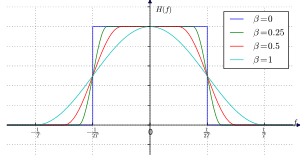
\includegraphics[width = 8cm]{media/Hf-Raised-cosine_filter.png}
            \caption{Funzione coseno rialzato: $G_{RCR(f)}$}
        \end{figure}
        all'aumentare di $\alpha$ la banda di nel dominio del tempo il coseno rialzato ha la forma
        \[
            g_{RCR(t)} = sinc(\frac{t}{T})\frac{cos(\alpha\pi\frac{t}{T})}{1-\frac{2\alpha t}{T}^2}  
        \]
        \begin{figure}[H]
            \centering
            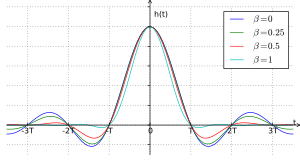
\includegraphics[width = 8cm]{media/ht-Raised-cosine-impulse.png}
            \caption{Funzione coseno rialzato: $g_{RCR(t)}$}
        \end{figure}
        ricordando una $sinc$ ma con lobi molto smorzati man mano che $\alpha$ tende a $1$. 

        Si sceglie il fattore di Roll-off tenendo conto sia della efficenza spettrale che migliora al decrescere di $\alpha$,
        dal dominio del tempo bisogna invece tener conto della sensibilitá all'ISI che diminuisce al crescere di $\alpha$.
        Inoltre una propietá del coseno rialzato é \label{propieta coseno rialzato} 
        \[
            g_{RCR(0)} = \int_{-\infty}^{\infty}G_{RCR(f)}df = 1
        \]
    \subsection{Filtro adattato}
        Ci poniamo adesso il problema del dimensionamento di $g_{(t)}$ in forma estesa, cioé
        dimensionando i filtri $g_{T(t)},g_{R(t)}$ nelle ipotesi che il canale sia $c_{(t)} = \delta_{(t)}$. 
        Il nostro obbiettivo é ridurre al minimo, se non eliminare, sia l'ISI che il rumore, per ottenere ció si introduce
        il fltro adattato (Matched Filter). Il filtro risolve il seguente problema: preso un impulso $p_{(t)}$ di forma nota,
        immerso in rumore additivo bianco $w_{(t)}$ (anche non Gaussiano) con densitá spettrale di potenza $S_{w(f)} = \frac{N_0}{2}$. 
        Il segnale é inviato in ingresso ad un sistema lineare e tempo invariante con risposta impulsiva $h_{(t)}$ e campionato ad un 
        istante $t_{0}$, ottenendo il campione $x_{(t_0)}$ come nel sistema di ricezione
        \begin{figure}[H]
            \centering
            \begin{tikzpicture}[
                    node distance=2cm,
                    >=latex
                ]
                % Blocks
                \node [coordinate,draw] (in) {};
                \node [circle, draw,right of=in] (TX) {$+$};
                \node [circle, draw,below of=TX] (WT) {$w_{(t)}$};
                \node [rectangle, draw,minimum height=3em, minimum width=4em,right of=TX] (C) {$h_{(t)}$};
                \node [rectangle, draw,minimum height=1em, minimum width=1em,right of=C] (RX) {$t_0$};
                \node [coordinate,right of = RX] (output) {};
            
                % Connections
                \draw [->] (in) --node[above]{$p_{(t)}$} (TX);
                \draw [->] (WT) -- (TX);
                \draw [->] (TX) --node[above]{$r_{(t)}$} (C);
                \draw [->] (C) --node[above]{$x_{(t)}$} (RX);
                \draw [->] (RX) --node[above]{$x_{(t_0)}$} (output);
            \end{tikzpicture}
        \end{figure}        
        Volgiamo quindi determinare $h_{(t)}$ in modo che sia massimo il rapporto segnale/rumore (SNR) sul campione $x_{t_0}$. Abbiamo 
        nel sistema
        \begin{gather}
            x_{(t)} = p_{(t)}\otimes h_{(t)}+w_{(t)}\otimes h_{(t)} = s_{(t)}+ n_{(t)}\nonumber \\
            \eval*{x_{(t)}}_{t=t_0} = s_{(t_0)} + n_{(t_0)}\nonumber
        \end{gather}
        esplicitando i valori
        \begin{gather}
            s_{(t_0)} = \int_{-\infty}^{\infty} h_{\tau} p_{(t_0-\tau)}d\tau \nonumber\\
            n_{(t_0)} = \int_{-\infty}^{\infty} h_{\tau} w_{(t_0-\tau)}d\tau \nonumber
        \end{gather}
        ricordiamo che $n_0$ é una variabile aleatoria e calcolando l'SNR:
        \[
            \frac{S_u}{N_u} = \frac{s^2_{t_0}}{\mathbb{E}[n^2_{(t_0)}]}  
        \]
        dove 
        \begin{align}
            \mathbb{E}[n^2_{(t_0)}] &= R_{n(0)} \overset{TCF}{=} S_{n(f)} = S_{w(f)}\left|H_{(f)}\right|^2 = \frac{N_0}{2}\left|H_{(f)}\right|^2 \nonumber \\
                                    &\overset{ATCF}{=} \int_{-\infty}^{\infty} S_{n(f)} df = \int_{-\infty}^{\infty} \frac{N_0}{2}\left|H_{(f)}\right|^2 df \nonumber            
        \end{align}
        essendo $H_{(f)}$ la trasformata di fourier di $h_{(t)}$ e tenendo conto del teorema di Parseval ho
        \[
            \mathbb{E}[n^2_{(t_0)}] = \frac{N_0}{2}\int_{-\infty}^{\infty} h_{(t)}^2 dt
        \]
        invece calcolando $s^2_{(t_0)}$ lo dobbiamo scegliere $h_{(t)}$ per massimizzare l'SNR e ridurre al minimo l'errore
        \begin{align}
            SNR &= \frac{s^2_{t_0}}{\frac{N_0}{2}\int_{-\infty}^{\infty} h_{(t)}^2 dt} = \frac{\int_{-\infty}^{\infty} h_{\tau} p_{(t_0-\tau)}d\tau}{\frac{N_0}{2}\int_{-\infty}^{\infty} h_{(t)}^2 dt} \nonumber \\
                &\overset{Dsg. Swartz}{\leq} \frac{\int_{-\infty}^{\infty} h_{\tau}d\tau \int_{-\infty}^{\infty} p_{(t_0-\tau)}d\tau}{\frac{N_0}{2}\int_{-\infty}^{\infty} h_{(t)}^2 dt} = \frac{2}{N_0}E_p \nonumber
        \end{align}        
        l'uguaglianza si ha se $h_{(t)} = kp_{(t_0-t)}$ con $k$ numero reale non nullo, ecco perché si chiama filtro adattato, poiché si adatta all'impulso $p_{(t)}$ e 
        massimizza il rapporto segnale rumore all'istante $t_0$ quando il rumore é bianco e la risposta impulsiva del filtro é 
        \[
            h_{(t)} = p_{(t_0-t)}  
        \]     
        cioé una versione del segnale $p_{(t)}$ ribaltata e traslata di $t_{0}$ come ad esempio 
        \begin{figure}[H]
            \centering
            \subfloat[$p_{(t)}$]{
                
\includegraphics[width=5.5cm]{media/uwu.png}
            }
            \hfill
            \subfloat[$p_{(t_0-t)}$]{
                
\includegraphics[width=5.5cm]{media/uwu.png}
            }
        \end{figure}
        Si puó ricavare la componente utile del segnale in uscita dal sistema
        \[
            s_{(t_0)} = \int_{-\infty}^{\infty} p{(t_0-t)}dt = E_p  
        \]
        e la risposta in frequenza del filtro adattato
        \[
            H_{(f)} = TCF[p_{(t_0-t)}] = P^*_{(f)}e^{-j2\pi ft_0}    
        \]
        con $P_(f) = TCF[p_{(t)}]$. Il modulo del filtro é 
        \[
            \left|H_{(f)}\right| = \left|P_{(f)}\right|   
        \] 
        si osserva come nel domino della frequenza il filtro adattato amplifichi le zone freqeunziali dove $ \left|P_{(f)}\right|$
        é maggiore (zona rapporto segnale rumore elevato) e attenui le zone freqeunziali dove $ \left|P_{(f)}\right|$ é minore 
        (zone a basso rapporto segnale romore), si adatta al segnale.

        \subsubsection{Progettazione dei filtri di ricezione e trasmissione}
            Nella raltá il canale $c_{(t)}$ é un canale distorcente diverso quindi da $\delta_{(t)}$, il dimensionamento di $g_{T(t)}$
            e $g_{R(t)}$. Tipicamente in pratica per il dimensionaemnto di $g_{T(t)}$ e $g_{R(t)}$ consiste nell'assumere il canale 
            come $c_{(t)} = \delta_{(t)}$ in modo tale che quando il canale non é distorcente il segnale venga trasmesso correttamente
            mentre se il canale diventa distorcente si prendereanno delle precauzioni al ricevitore per mitigare tali distorsioni.
            Supponiamo quindi che il canale sia $c_{(t)} = \delta_{(t)}$ gli impulsi in ingresso al filtro di ricezione saranno del tipo
            \[
                g_{TC(t)} = g_{T(t))} \otimes c_{(t)} =  g_{T(t))} 
            \]
            e la risposta impulsiva globale del sistema PAM
            \[
                g_{(t)} = g_{TC(t))} \otimes g_{R(t)} =  g_{T(t))} \otimes g_{R(t)}
            \]
            abbiamo 2 variabili, $g_{T(t)}$ e $g_{R(t)}$, e dobbiamo rispettare 2 condizioni (é un problema di ricerca dell'ottimo):
            \begin{enumerate}
                \item {
                    Annullamento dell'ISI: Dobbiamo fare in modo che $g_{(t)}$ sia un impulso che soddisfi le condizioni di Nyquist,
                    tipicamente un impulso a coseno rialzato
                    \[
                        G_{(f)} = G_{T(f)} G_{R(f)} = G_{RCR(f)} 
                    \]
                }
                \item {
                    Massimizzare il rapporto Segnale/Rumore sul campionatore in uscita dal filtro di ricezione:
                    si deve fare in modo che il filtro in ricezione $g_{R(t)}$ sia adattato agli impulsi presenti al suo ingresso
                    \[
                        g_{R(t)} = g_{T(-t)} \Rightarrow G_{R(f)} = G_{T(f)}^\ast
                    \]
                    in caso il canale fosse $c_{(t)} \neq \delta_{(t)}$ 
                    \[
                        G_{R(f)} = G_{T(f)}^\ast = \left[G_{T(f)} C_{(f)}\right]^\ast  
                    \]                
                }
            \end{enumerate}
            unendo le due condizioni 
            \[
                G_{RCR(f)} = G_{T(f)}G_{T(f)}^\ast = \left|G_{T(f)}\right|^2  
            \]
            dato che la funzione coseno rialzato é reale e non negativa posso esprimere la $G_{T(f)}$ come
            \[
                G_{T(f)} = \sqrt{G_{RCR(f)}} = G_{R(f)}    
            \] 
            cioé le risposte in frequenza dei filtri in trasmissione e ricezione coincidono cone la radice
            quadrata della funzione coseno rialzato. I corrispondenti impulsi nel dominio del tempo 
            $g_{T(t)}$ e $g_{R(t)}$ sono detti \emph{impulsi a radice di coseno rialzato} e con l'acronimo RRCR
            (Root raised cosine Roll-off). Si puó notare come non siano impulsi di Nyquist ma la loro convoluzione 
            invece si.
            \begin{figure}[H]
                \centering
                \subfloat[$g_{RRCR(t)}$]{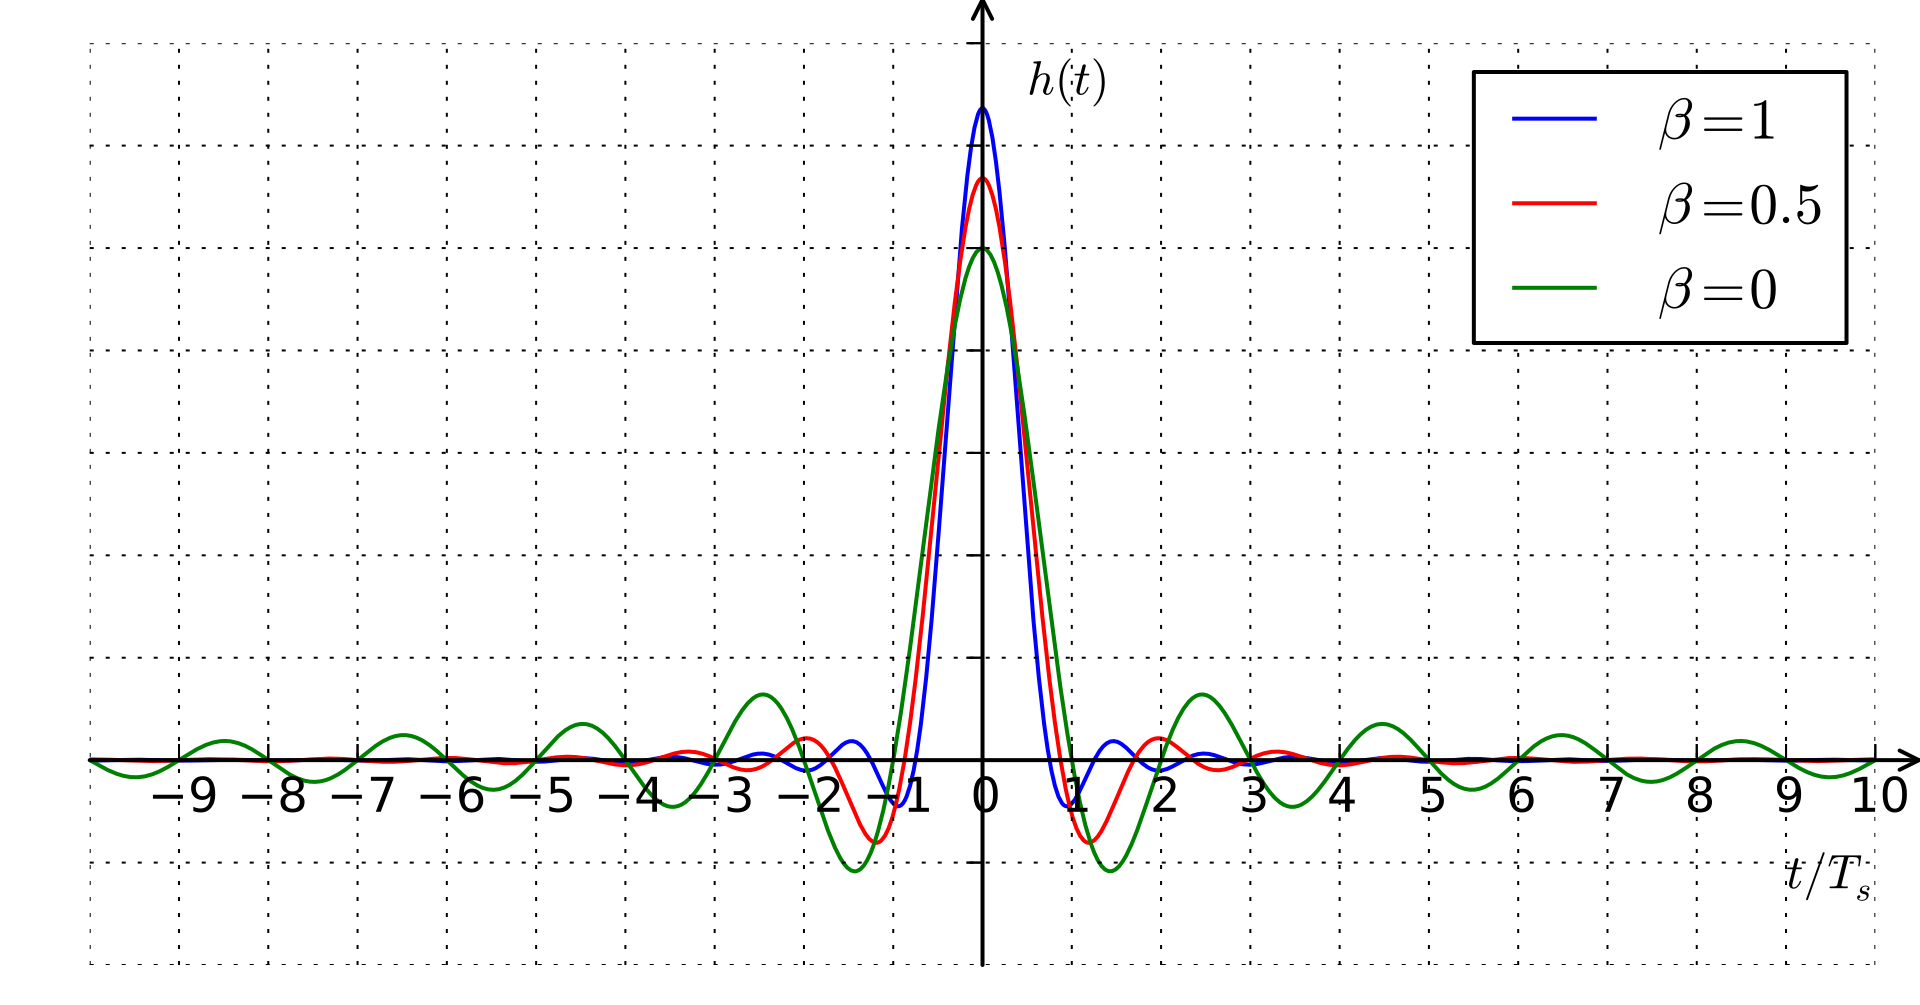
\includegraphics[width = 6cm]{media/Root-raised-cosine-impulse.png}}
                \hfill
                \subfloat[$G_{RRCR(f)}$]{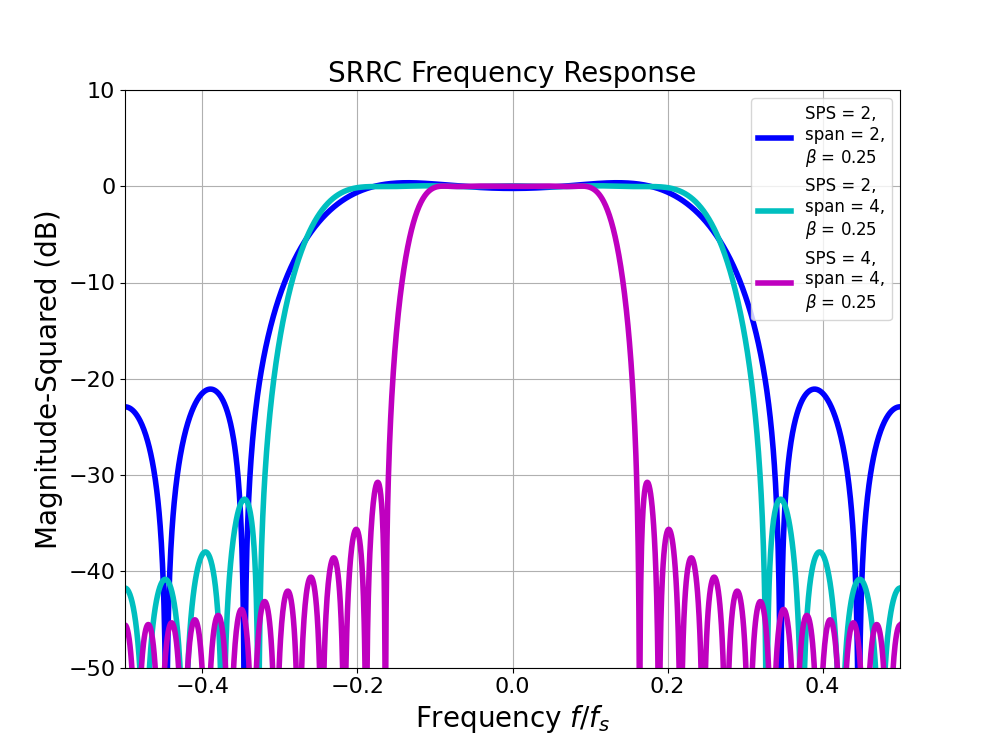
\includegraphics[width = 6cm]{media/srrcDesign_frequencyResponse-1.png}}
            \end{figure}           
            ha gli stessi punti di discesa e valori della funzione a coseno rialzato.
    \subsection{Circuito decisore}
        Siamo giunti al decisore del nostro sistema di comunicazione
        \begin{figure}[H]
            \centering
            \begin{tikzpicture}[
                    node distance=3cm,
                    >=latex
                ]
                % Blocks
                \node [coordinate,draw] (in) {};
                \node [rectangle, draw,right of=in] (C) {$kT$};
                \node [rectangle, draw,minimum height=1em, minimum width=1em,right of=C] (RX) {$Decisore$};
                \node [coordinate,right of = RX] (output) {};
            
                % Connections
                \draw [->] (in) --node[above]{$x_{(t)}$} (C);
                \draw [->] (C) --node[above]{$x_{[k]}$} (RX);
                \draw [->] (RX) --node[above]{$\hat{a}_{k}$} (output);
            \end{tikzpicture}
        \end{figure}        
        il decisore riceve al suo ingresso il campione $x_{[k]}$ e lo utilizza per prendere una decisione sul simbolo trasmesso
        $a_k$ usando il criterio di ottimalitá.
        \paragraph{Criterio MAP}
            Il criterio che minimizza la probabilitá di errore sul simbolo $a_k$ é detto criterio MAP (Maximum A-posterior Probability),
            secondo tale criterio il simbolo da scegliere all'interno dell'alfabeto $\mathcal{A} = \{a^{(1)},a^{(2)},\dots,a^{(M)}\}$
            é quello che ha il massimo probabiltá a posteriori di essere stato trasmesso, cioé dopo aver osservato il campione $x_{[k]}$.
            Il criterio MAP sancisce quindi 
            \[
                P_r[a_k = a^{(i)}|x_{[k]}]    
            \]
            la probabilitá di aver trasmesso $\hat{a}_{k}=a^{(i)}$ nell'ipotesi di aver ricevuto $x_{[k]}$, questa sará
            \[
                P_r[a_k = a^{(i)}|x_{[k]}] \leq P_r[a_k = a^{(\ell)}|x_{[k]}]\ \forall i\neq \ell\in \{1,2,\dots,M\}    
            \]
            é minore della probabilitá di scegliere un simbolo $a^{(\ell)}$ sbagliato. Voglio massimizzare la prbabilitá di 
            corretta ricezione 
            \[
                P_r[a_k = a^{(i)}|x_{[k]}] = \frac{f_x[x_{[k]}|a_k = a^{(i)}]P_r[a_k = a^{(i)}]}{f_x[x_{[k]}]}    
            \]
            dove $f_x[x_{[k]}]$ é la funzione densitá di probabilitá del campione $x_{[k]}$,
            é come la probabilitá di Bayes (\ref{Regola di Bayes}) ma con la densitá di probabilitá ($fdp$). Posso analizzare
            solo il numeratore poiché dipende dal simbolo trasmesso, definisco quindi 
            \[
                \gamma_{(a^{(i)},x_{[k]})} = f_x[x_{[k]}|a_k = a^{(i)}]P_r[a_k = a^{(i)}]
            \] 
            ho $\hat{a}_k = a^{(i)}$ se 
            \[
                \gamma_{(a^{(i)},x_{[k]})} > \gamma_{(a^{(\ell)},x_{[k]})}
            \]
            se il numeratore della probabilitá di corretta ricezione é maggiore di quello di sbagliata ricezione, 
            analizzo i due nuemratori nelle ipotesi di 
            \begin{itemize}
                \item {ISI$=0$}
                \item {$c_{(t)} = \delta_{(t)}$ oppure $c_{(t)} = A\delta_{(t-\tau)}$, non cambia tra i due il secondo tipo di canale campiona a $kT+\tau$
                    che é il segnale ritardato}
                \item {$g_{(t)} = g_{TxRCR(t)}\otimes g_{RxRCR(t)} + n_{[k]}$}
            \end{itemize}
            Ho quindi 
            \[
                x_{[k]} \overset{ISI=0}{=} a_kg_{(0)} + n_{[k]} = a_k + (n_{[k]} \sim \mathcal{N}(0,\sigma_n^2))
            \]
            dove 
            \[
                \sigma_n^2 = \int_{-\infty}^{\infty}S_{n(f)}df = \frac{N_0}{2} \int_{-\infty}^{\infty}\underset{\ref{propieta coseno rialzato}}{\left| G_{R(f)} \right|} df = \frac{N_0}{2}  
            \]
            e la funzione densitá di probabilitá 
            \begin{gather}
                f_x[x_{[k]}|a_k = a^{(i)}] = \frac{1}{\sqrt{2\pi}\sigma_n}e^{\left(\displaystyle -\frac{(x_{[k]}-a^{(i)})^2}{2\sigma_n^2}\right)} \nonumber \\
                x_{[k]} | a_k = a^{(i)} \sim \mathcal{N}(a^{(i)},\sigma_n^2)\nonumber \\
                f_x[x_{[k]}|a_k = a^{(i)}] = \Gamma_{(a^{(i)},x_{[k]})} \nonumber
            \end{gather}
            massimizziamo adesso $\gamma_{(a^{(i)},x_{[k]})}$ con l'ipotesi che i simboli siano equiprobabili $P_r[a^{(i)}] = \frac{1}{M}$. Allora anche il termine
            $P_r[a_k = a^{(i)}]$ diventa trascurabile per la massimizzazione, ne rimane quindi solo da massimizzare
            \[
                \Gamma_{(a^{(i)},x_{[k]})} > \Gamma_{(a^{(\ell)},x_{[k]})}    
            \]
            essendo funzioni monotone decrescenti posso farne il logaritmo naturale
            \begin{gather}
                ln\left(\Gamma_{(a^{(i)},x_{[k]})} \right)> ln\left(\Gamma_{(a^{(\ell)},x_{[k]})}\right) \nonumber\\
                \frac{-\left(x_{[k]}-a^{(i)}\right)^2}{2\sigma_n^2}-ln\left(\sqrt{2\pi}\sigma_n\right) >  \frac{-\left(x_{[k]}-a^{(\ell)}\right)^2}{2\sigma_n^2}-ln\left(\sqrt{2\pi}\sigma_n\right)\nonumber \\
                \left(x_{[k]}-a^{(i)}\right)^2<\left(x_{[k]}-a^{(\ell)}\right)^2\nonumber    
            \end{gather}
            il risultato trovato é la distanza euclidea del simbolo ricevuto minore della distanza euclidea da qualsiasi altro simbolo. Se
            questa disuguaglianza é vera, é il criterio chiamato a distanza minima euclidea o a massima verosomiglianza, valido solo se i simboli
            sono equiprobabili. Ho due criteri 
            \[
                MAP \overset{\text{Se equiprobabili}}{\Rightarrow} \text{Massima verosomiglianza}  
            \] 
            nel caso MAP massimizzo la funzione $\gamma_{(a^{(i)},x_{[k]})}$, nel caso a massima verosomiglianza massimizzo la $\Gamma_{(a^{(i)},x_{[k]})}$ 
            In caso di simboli non equiprobabili si arriva alla funzione 
            \[
                \Gamma_{(a^{(i)},x_{[k]})} = \left[x_{[k]}-a^{(i)}\right]^2-2\sigma^2ln(P_i)
            \]
            con $P_i$ probabilitá a priori del simbolo $a^{(i)}$
        \subsubsection{Zone di decisione}
            Il criterio MAP suddivide l'asse reale in \emph{zone di decisione}, ciascuna associata a un determinato simbolo dell'alfabeto $\mathcal{A}$.
            Indichiamo con $\mathcal{Z}^{(m)}$ la zona di decisione associata al simbolo $a^{(m)}\in\mathcal{A}$, essa é definita come
            \[
                \mathcal{Z}^{(m)} = \left\{ x\in\mathbb{R}: \Gamma_{(a^{(m)},x_{[k]})}<\Gamma_{(a^{(\ell)},x_{[k]})}, a^{(\ell)}\in\mathcal{A} \vee a^{(\ell)}\neq a^{(m)} \right\}
            \]   
            per cui la decisione $\hat{a}_{k}$ viene presa a favore del simbolo $a^{(i)}$ solo se $x_{[k]}\in \mathcal{Z}^{(i)}$. Il decisore altro non é 
            che un comparatore di $x_{[k]}$ con delle soglie in modo da individuare la zona di decisione di $x_{[k]}$. 
            \paragraph{Esempio PAM $\mathcal{A} = \{-1,+1\}$}{
                Prendiamo in esempio una PAM con alfabeto $\mathcal{A} = \{-1,+1\}$ e sia 
                \[
                    p=P_r[a_k=-1]\ e\ 1-p=P_r[a_k=+1]
                \]
                scegliamo il decisore sulla base del criterio MAP e ipotizziamo di dover scegliere per il simbolo $\hat{a}_k =+1$ se
                \[
                    \Gamma_{(+1,x_{[k]})} < \Gamma_{(-1,x_{[k]})} 
                \]  
                svolgendo i calcoli nel caso di simboli non equiprobabili
                \begin{gather}
                    \left[x_{[k]}-1\right]^2-2\sigma^2ln(1-p)<\left[x_{[k]}+1\right]^2-2\sigma^2ln(p)\nonumber \\
                    x_{[k]}> \frac{\sigma^2}{2}ln\left(\frac{p}{1-p}\right) = \lambda\nonumber
                \end{gather}
                \begin{figure}[H]
                    \centering
                    \begin{tikzpicture}
                        \begin{axis}[
                            xlabel=$x$,
                            % ylabel=$\lambda=\frac{\sigma^2}{2}ln\left(\frac{p}{1-p}\right)$,
                            xmin=-3,
                            xmax=3,
                            ymin=-1,
                            ymax=1.3,
                            % ytick = {},
                            % yticklabels = {},
                            xtick={-1.5,1.5},
                            xticklabels={$-1$,$+1$},
                            axis x line=middle,
                            axis y line=none,
                            domain=3:3,
                            samples=800,
                            width=12cm,
                            height=5cm
                        ]
                            \node [] at (-1.5,0.5) {\small\text{Zona di decisione }$\hat{a}_k =-1$};
                            \node [] at (1.5,0.5) {\small\text{Zona di decisione }$\hat{a}_k =+1$};
                            \node [] at (0.8,1) {\small$\lambda=\frac{\sigma^2}{2}ln\left(\frac{p}{1-p}\right)$};
                            \addplot [orange,thick, dotted] coordinates{(0,-1)(0,1.5)};

                        \end{axis}
                    \end{tikzpicture}
                    \caption{Zone di decisione PAM $\mathcal{A} = \{-1,+1\}$}
                \end{figure}
                l'asse é stato suddiviso in due zone di decisione e la soglia $\lambda$ dipende da $\sigma^2$ e $p$.
                Possiamo anche analizzare l'andamento di $\lambda$ al variare di $p$ fissato un valore di $\sigma$
                \begin{figure}[H]
                    \centering
                    \begin{tikzpicture}
                        \begin{axis}[
                            xlabel=$p$,
                            ylabel=$\lambda$,
                            xmin=-0.1,
                            xmax=1.5,
                            ymin=-3,
                            ymax=3,
                            ytick = {},
                            yticklabels = {},
                            xtick={0.5,1},
                            xticklabels={$\frac{1}{2}$,$1$},
                            axis lines=middle,
                            domain=0:5,
                            samples=800,
                            width=8cm,
                            height=10cm
                        ]
                        \addplot [black, const plot, thick,samples=1200] {0.5*ln(x/(1-x))};
                        \addplot [orange, dotted, thick] coordinates{(1,-3)(1,3)};
                    \end{axis}
                    \end{tikzpicture}
                \end{figure}
                come si vede nel caso di simboli equiprobabili $p=\frac{1}{2}$ la soglia vale $\lambda=0$, mentre
                assume valori positivi se la probabilitá del simbolo $\hat{a}_k = -1$ é $p>\frac{1}{2}$ ha maggiore 
                probabilitá a priori di essere trasmesso. Il decisore tende a privilegiare la decisione sul simbolo
                che ha maggiore probabilitá a priori di essere trasmesso, allargandone opportunemante la relativa
                zona di decisione.
            }
            
            Consideriamo il caso pratico in cui i simboli dall'alfabeto $\mathcal{A} = \{a^{(1)},\dots,a^{(M)}\}$ siano
            equiprobabili
            \[
                P_m=\frac{1}{M}\ m=1,\dots,M  
            \]
            in questo caso il termine $-2\sigma^2ln(P_m)$ non dipende da $a^{(m)}$ e diventa trascurabile per la decisione
            di $a_k$, il criterio di decisione si riduce alle distanze euclidee e il criterio a \emph{massima verosomiglianza}, $\hat{a}_k=a^{(i)}$ se
            \[
                \Gamma_{(a^{i},x_{[k]})} < \Gamma_{(a^{(\ell)},x_{[k]})}                    
            \]
            che diventano 
            \[
                \left(x_{[k]}-a^{(i)}\right)^2<\left(x_{[k]}-a^{(\ell)}\right)^2  
            \]
            in caso di simboli equiprobabili possiamo notare che le soglie di decisione siano posizionate esattamente a 
            metá tra i due simboli adiacenti dell'alfabeto, ad esempio in un sistema PAM quaternario
            \begin{figure}[H]
                \centering
                \begin{tikzpicture}
                    \begin{axis}[
                        xlabel=$x$,
                        % ylabel=$\lambda=\frac{\sigma^2}{2}ln\left(\frac{p}{1-p}\right)$,
                        xmin=-5,
                        xmax=5,
                        ymin=-1,
                        ymax=1,
                        % ytick = {},
                        % yticklabels = {},
                        xtick={-3,-1,1,3},
                        xticklabels={$-3$,$-1$,$+1$,$+3$},
                        axis x line=middle,
                        axis y line=none,
                        domain=5:5,
                        samples=100,
                        width=12cm,
                        height=5cm
                    ]
                        \node [] at (-1,0.5) {\small$\hat{a}_k =-1$};
                        \node [] at (-3,0.5) {\small$\hat{a}_k =-3$};
                        \node [] at (1,0.5) {\small$\hat{a}_k =+1$};
                        \node [] at (3,0.5) {\small$\hat{a}_k =+3$};
                        \addplot [orange,thick, dotted] coordinates{(0,-1)(0,1)};
                        \addplot [orange,thick, dotted] coordinates{(2,-1)(2,1)};
                        \addplot [orange,thick, dotted] coordinates{(-2,-1)(-2,1)};
                    \end{axis}
                \end{tikzpicture}
                \caption{Zone di decisione 4-PAM $\mathcal{A} = \{-3,-1,+1,+3\}$}
            \end{figure}
            il simbolo deciso dall'alfabeto $\mathcal{A}$ sará pertanto quello che ha distanza euclidea minore rispetto al 
            campione $x_{[k]}$ ricevuto. Il criterio a massima verosomiglianza quindi minimizza l'errore in caso 
            di simboli equiprobabili e a discapito della conoscenza di $\sigma$ e la probabilitá dei simboli,
            possiamo anche utilizzarlo in caso di simboli non equiprobabili fornendoci una soluzione sub-ottima. 
        \subsubsection{Calcolo della SER per un sistema PAM M-ario}
            Consideriamo un sistema PAM con alfabeto M-ario
            \[
                \mathcal{A} = \{\pm 1,\pm 3,\dots, \pm(M-1)\}  
            \]
            il sistema M-PAM ottiene $x_{[k]} = Aa_k + n_{[k]}$,
            vogliamo calcolare la probabilitá media di errore sul simbolo deciso ammettendo che i simboli 
            siano equiprbabili, in assenza di ISI all'ingresso del ricevitore cosí fatto
            \begin{figure}[H]
                \centering
                \begin{tikzpicture}[
                        node distance=3cm,
                        >=latex
                    ]
                    % Blocks
                    \node [coordinate,draw] (in) {};
                    \node [rectangle, draw,minimum height=2em, minimum width=2em,right of=in] (C) {$g_{R(t)}$};
                    \node [rectangle, draw,minimum height=2em, minimum width=2em,right of=C] (camp) {$kT$};
                    \node [rectangle, draw,minimum height=2em, minimum width=2em,right of=camp] (RX) {$Decisore$};
                    \node [coordinate,right of = RX] (output) {};
                
                    % Connections
                    \draw [->] (in) --node[above]{$r_{(t)}$} (C);
                    \draw [->] (C) --node[above]{$x_{(t)}$} (camp);
                    \draw [->] (camp) --node[above]{$x_{[k]}$} (RX);
                    \draw [->] (RX) --node[above]{$\hat{a}_{k}$} (output);
                \end{tikzpicture}
            \end{figure}                    
            supponiamo che i filtri in trasmissione e ricezione siano entrambi a radice di coseno rialzato. Il problema di questa 
            approssimazione del sistema é che si suppone un canale di trasmissioene $\delta_{(t)}$ quando in realtá si approssima
            meglio con $A\delta_{(t-\tau)}$, dobbiamo quindi campionare a $kT+\tau$ e scalare per $A$, valori che saranno 
            opportunamente ricevuti al momento della sincronizzazione, il sistema diventa 
            \begin{figure}[H]
                \centering
                \begin{tikzpicture}[
                        node distance=2cm,
                        >=latex
                    ]
                    % Blocks
                    \node [coordinate,draw] (in) {};
                    \node [circle, draw,right of=in] (scale) {$\times$};
                    \node [circle, draw,below of=scale] (factor) {$\frac{1}{A}$};
                    \node [rectangle, draw,minimum height=1em, minimum width=1em,right of=scale] (C) {$g_{R(t)}$};
                    \node [rectangle, draw,minimum height=1em, minimum width=1em,right of=C] (camp) {$kT+\tau$};
                    \node [rectangle, draw,minimum height=1em, minimum width=1em,right of=camp] (RX) {$Decisore$};
                    \node [coordinate,right of = RX] (output) {};
                
                    % Connections
                    \draw [->] (in) --node[above]{$r_{(t)}$} (scale);
                    \draw [->] (factor) -- (scale);
                    \draw [->] (scale) --node[above]{$\frac{r_{(t)}}{A}$} (C);
                    \draw [->] (C) --node[above]{$z_{(t)}$} (camp);
                    \draw [->] (camp) --node[above]{$z_{[k]}$} (RX);
                    \draw [->] (RX) --node[above]{$\hat{a}_{k}$} (output);
                \end{tikzpicture}
            \end{figure}                    
            dove $z_{[k]} = \frac{x_{[k]}}{A} = a_k + \frac{n_{[k]}}{A}$ il rumore é quindi $\simeq\mathcal{N}(0,\frac{\sigma^2_n}{A^2})$, se calcoliamo
            la varianza nel caso della PAM con simboli indipendenti 
            \[
                \sigma_n^2 = \frac{\sigma^2_n}{A^2} = \frac{N_0}{2}\frac{M^2-1}{3E_s}= \frac{M^2-1}{6(\frac{E_s}{N_0})}    
            \] 
            Se non scalassi per il fattore $A$ le zone di decisione dovrebebro adattarsi al valore di $A$.
            Il decisore suddivide l'asse $x$ in zone di decisione, come mostrato in figura 131, con le soglie poste esattamente
            a metá tra due simboli adiacenti nel caso di simboli equiprobabili
            \begin{figure}[H]
                \centering
                \begin{tikzpicture}
                    \begin{axis}[
                        xlabel=$x$,
                        % ylabel=$\lambda=\frac{\sigma^2}{2}ln\left(\frac{p}{1-p}\right)$,
                        xmin=-6,
                        xmax=6,
                        ymin=-1,
                        ymax=1,
                        % ytick = {},
                        % yticklabels = {},
                        xtick={-5,-3,-1,1,3,5},
                        xticklabels={$-(M-1)$,$-(M-3)$,$\dots$,$\dots$,$M-3$,$M-1$},
                        axis x line=middle,
                        axis y line=none,
                        domain=5:5,
                        samples=100,
                        width=12cm,
                        height=5cm
                    ]
                        \node [] at (-5,0.5) {\small$a^{(1)}$};
                        \node [] at (-3,0.5) {\small$a^{(2)}$};
                        \node [] at (-1,0.5) {\small$\dots$};
                        \node [] at (1,0.5) {\small$\dots$};
                        \node [] at (3,0.5) {\small$a^{(M-1)}$};
                        \node [] at (5,0.5) {\small$a^{(M)}$};
                        \addplot [orange,thick, dotted] coordinates{(0,-1)(0,1)};
                        \addplot [orange,thick, dotted] coordinates{(2,-1)(2,1)};
                        \addplot [orange,thick, dotted] coordinates{(4,-1)(4,1)};
                        \addplot [orange,thick, dotted] coordinates{(-2,-1)(-2,1)};
                        \addplot [orange,thick, dotted] coordinates{(-4,-1)(-4,1)};
                    \end{axis}
                \end{tikzpicture}
                \caption{Zone di decisione M-PAM $\mathcal{A} = \{\pm 1,\pm 3,\dots, \pm(M-1)\}$}
            \end{figure}
            usando il teorema della probabilitá totale possiamo esprimere la SER (Symbol Error Rate)
            \[
                SER = \sum_{i=1}^{M}P[e|a^{(m)}]P_r[a_k=a^{(i)}]    
            \]
            dove 
            \[
                P[e|a^{(m)}] = P_r[\hat{a}_k \neq a_k | a_k=a^{(m)}]
            \]
            nell'ipotesi di simboli equiprobabili
            \[
                SER = \frac{1}{M} \sum_{m=1}^{M}P[e|a^{(m)}]  
            \]
            restano quindi da calcolare le $M$ probabilitá condizionate $P[r|a^{(m)}]$ per $m = 1,\dots,M$.
            L'analisi dell'alfabeto $\mathcal{A}$ e le zone di decisione si puó eveincere come i simboli 
            nelle zone di decisione esterne ($\pm(M-1)$) abbiano la stessa probabilitá, come anche i 
            simboli interni $\{\pm 1,\dots,\pm (M-3)\}$ abbiano tra di loro la stessa probabilitá. Ne segue che 
            possiamo calcolare solo due probabilitá, ad esempio
            \begin{gather}
                P[e|a^{(m)}] = P[e|a_k = 1]\ se\ a^{(m)\in\{\pm 1,\dots,\pm (M-3)\}}\nonumber \\
                P[e|a_k =-M+1] = P[e|a_k = M-1]\ se\ a^{(m)\in\{\pm (M-1)\}}\nonumber
            \end{gather}
            da cui ricaviamo la SER finale del sistema
            \[
                SER =  \frac{M-2}{M}P[e|a_k = 1]+ \frac{2}{M}P[e|a_k = M-1]
            \]
            dove i coefficienti moltiplicativi sono quanti simboli hanno la relativa probabilitá, ricordiamoci
            che possiamo fare cosí solo perché la costellazione lo permette, magari in casi diversi potrei
            avere piú termini. Il nostro simbolo trasmesso é quindi caratterizzato da
            \[
                z_{[k]} = a_{[k]} + \eta_{[k]}
            \]
            con $\eta_{[k]} = \frac{n_{[k]}}{A} \sim \mathcal{N}(0,\frac{\sigma_n^2}{A^2})\sim \mathcal{N}(0,\sigma_\eta^2)$,
            per un generico simbolo la sua probabilitá di errore é espressa come 
            \[
                P_{err} = Q_{\displaystyle\left(\frac{\lambda - a^{(m)}}{\sigma}\right)}    
            \]
            dove $\lambda - a^{(m)}$ indica la distanza dalla soglia.
            Calcoliamo le probabilitá di errore condizionale:
            \begin{enumerate}
                \item {Calcolo di $P[e|a_k = 1]$
                    Supponiamo sia stato inviato il simbolo $a_k = 1$ il campione ricevuto é 
                    \[
                        z_{[k]} = 1 + \eta_{[k]}  
                    \]
                    \begin{figure}[H]
                        \centering
                        \begin{tikzpicture}
                            \begin{axis}[
                                xlabel=$x$,
                                ylabel=$a$,
                                xmin=-5,
                                xmax=5,
                                ymin=-1,
                                ymax=1,
                                ytick = {},
                                yticklabels = {},
                                xtick={-3,-1,1,3},
                                xticklabels={$\dots$,$-1$,$+1$,$\dots$},
                                axis x line=middle,
                                axis y line=middle,
                                domain=5:5,
                                samples=100,
                                width=12cm,
                                height=5cm
                            ]
                                \node [] at (-1,0.65) {\small$\hat{a}_k =-1$};
                                \node [] at (-3,0.65) {\small$\dots$};
                                \node [] at (1,0.65) {\small$\hat{a}_k =+1$};
                                \node [] at (3,0.65) {\small$\dots$};
                                \addplot [const plot,blue,thick, samples = 300, domain = -4:4] {gauss(1,0.8)};
                                \addplot [const plot,blue,name path = A, samples = 300, domain = -4:0] {gauss(1,0.8)};
                                \addplot [const plot,blue,name path = B, samples = 300, domain = 2:4] {gauss(1,0.8)};
                                \addplot [orange,thick, dotted] coordinates{(0,-1)(0,1)};
                                \addplot [orange,thick, dotted] coordinates{(2,-1)(2,1)};
                                \addplot [orange,thick, dotted] coordinates{(-2,-1)(-2,1)};
                                \addplot [black,const plot,name path = C] coordinates{(2,0)(4,0)};
                                \addplot [black,const plot,name path = D] coordinates{(0,0)(-4,0)};
                                \addplot[red,opacity = 0.3] fill between[of=A and D];
                                \addplot[red,opacity = 0.3] fill between[of=B and C];
                        \end{axis}
                        \end{tikzpicture}
                    \end{figure}
                    notiamo come l'errore é presente quando il simbolo non é compreso all'interno dell'intervallo
                    \begin{align}
                        P[e|a_k =1] &= P_r[z_{[k]}< 0 \cup z_{[k]}> 2] = P_r[1+\eta_{[k]}< 0 \cup 1+\eta_{[k]}> 2] \nonumber \\
                                    &= P_r[\eta_{[k]}< -1 \cup \eta_{[k]}> 1]\nonumber 
                    \end{align}
                    potremmo calcolare l'integrale della distribuzione di probabilitá ma utilizziamo la funzione $Q$,
                    gli intervalli di errore esterni sono uguali quindi possiamo calacolare $Q$ solo nel punto destro
                    \[
                        P[e|a_k =1] = 2Q_{\displaystyle\left(\frac{1}{\sigma_\eta}\right)}  
                    \]
                    
                }
                \item {Calcolo di $P[e|a_k = M-1]$
                    Supponiamo di aver trasmessio il simbolo $a_k = M-1$, il campione é caratterizzato da
                    \[
                        z_{[k]} = M-1+\eta_{[k]}    
                    \]
                    \begin{figure}[H]
                        \centering
                        \begin{tikzpicture}
                            \begin{axis}[
                                xlabel=$x$,
                                ylabel=$a$,
                                xmin=-5,
                                xmax=5,
                                ymin=-1,
                                ymax=1,
                                ytick = {},
                                yticklabels = {},
                                xtick={-3,-1,1,3},
                                xticklabels={$-M+1$,$\dots$,$\dots$,$M-1$},
                                axis x line=middle,
                                axis y line=middle,
                                domain=5:5,
                                samples=100,
                                width=12cm,
                                height=5cm
                            ]
                                \node [] at (-3,0.65) {\small$\hat{a}_k =-M+1$};
                                \node [] at (-1,0.65) {\small$\dots$};
                                \node [] at (3,0.65) {\small$\hat{a}_k =M-1$};
                                \node [] at (1,0.65) {\small$\dots$};
                                \addplot [orange,thick, dotted] coordinates{(0,-1)(0,1)};
                                \addplot [orange,thick, dotted] coordinates{(2,-1)(2,1)};
                                \addplot [orange,thick, dotted] coordinates{(-2,-1)(-2,1)};

                                \addplot [const plot,blue,thick, samples = 300, domain = 0:5] {gauss(3,0.8)};
                                \addplot [const plot,blue,name path = A, samples = 300, domain = 0:2] {gauss(3,0.8)};
                                \addplot [black,const plot,name path = B] coordinates{(0,0)(2,0)};
                                \addplot[red,opacity = 0.3] fill between[of=A and B];
                        \end{axis}
                        \end{tikzpicture}
                    \end{figure}
                    ho errore quando il simbolo non rientra nella semiretta $[M-2,+\infty]$
                    \begin{align}
                        P[e|a_k=M-1] &= P_r[z_{[k]}<M-2] = P_r[M-1+\eta_{[k]}<M-2] = P_r[\eta_{[k]}<-1] \nonumber \\
                                     &= P_r[\eta_{[k]}>1]\nonumber
                    \end{align}
                    dalla figura possiamo ricavare la probabilitá di errore 
                    \begin{align}
                        P[e|a_k=M-1] &= 1-Q_{\displaystyle \left(\frac{\lambda-a^{(m)}}{\sigma_\eta}\right)} = 1-Q_{\displaystyle\left(-\frac{1}{\sigma_\eta}\right)} \nonumber \\
                                     &= Q_{\displaystyle\left(\frac{1}{\sigma_\eta}\right)} \nonumber
                    \end{align}
                }
            \end{enumerate}
            Sostituiendo i risultati ottenuti nella formula della SER
            \begin{align}
                SER &= \frac{M-2}{M}2Q_{\displaystyle\left(\frac{1}{\sigma_\eta}\right)}+ \frac{2}{M}Q_{\displaystyle\left(\frac{1}{\sigma_\eta}\right)} \nonumber \\
                    &= \frac{2(M-1)}{M} Q_{\displaystyle\left(\frac{1}{\sigma_\eta}\right)} \nonumber
            \end{align}
            se la vogliamo esprimere in funzione del valore di $\sigma_\eta= \frac{\sigma_n^2}{A^2} = \frac{N_0}{2A^2}$
            \[
                SER = \frac{2(M-1)}{M} Q_{\displaystyle\left(\sqrt{\frac{2A^2}{N_0}}\right)} 
            \]
            Vogliamo adesso esprimere la SER in funzione dell energia del segnale ricevuto, prendiamo il segnale 
            ricevuto non filtrato 
            \[
                r_{(t)} = S_{R(t)} + w_{(t)} = \sum_{i}Aa_ig_{T(t-iT)}+w_{(t)}    
            \]
            la cui densitá spettrale di potenza é espressa come
            \[
                S_{R(f)} = \frac{A}{T}S_{a(f)}\left|G_{T(f)}\right|^2
            \]
            se i simboli sono independenti ed equiprobabili e sono nel caso di una PAM posso esprimere 
            densitá spettrale di potenza dei simboli come
            \begin{align}
                S_{a(f)} &= \sum_{m}R_{a(m)}e^{-j2\pi fmT} = R_{a(0)}\nonumber \\
                         &= E[a_m^2] = \frac{M^2-1}{3}\nonumber
            \end{align}
             
            allora $S_{R(f)}$ diventa
            \[
                S_{R(f)} = \frac{A}{T}\frac{M^2-1}{3}\left|G_{T(f)}\right|^2
            \]
            dalla quale possiamo calcolare l'energia dei simboli moltiplicando pet $T$ o dei bit 
            moltiplicando per $T_d$ 
            \[
                E_{simboli} = \int_{-\infty}^{\infty}S_{R(f)} df \overset{\ref{propieta coseno rialzato}}{=} A^2\frac{M^2-1}{3}  
            \]
            $A$ puó essere quindi espresso in funzione dell'energia dei simboli 
            \[
                A^2 = \frac{3E_{simboli}}{M^2-1} 
            \]  
            la SER espressa tramite l'energia del simbolo ricevuto é
            \[
                SER = \frac{2(M-1)}{M} Q_{\displaystyle\left(\sqrt{\frac{6E_{simboli}}{(M^2-1)N_0}}\right)} 
            \]
            nel caso di una PAM binaria 
            \[
                SER \overset{M=2}{=} Q_{\displaystyle\left(\sqrt{\frac{2E_{simboli}}{N_0}}\right)} 
            \]
        \subsubsection{Efficenza spettrale ed efficenza energetica}
            Abbiamo visto come l'impulso di trasmissione $g_{T(t)}$ impiegato in un sistema PAM sia tipicamente 
            un impulso a Radice di Coseno RIalzato (\ref{F. Coseno Rialzato}). Nel caso di simboli indipendenti
            ed equiprobabili, la densitá spettrale di potenza del segnale trasmesso é 
            \[
                S_{s(f)} = \frac{M^2-1}{3T}\left|G_{T(f)}\right|^2 = \frac{M^2-1}{3T} G_{RCR(f)}
            \]
            per cui la banda impiegata dal segnale PAM é 
            \[
                B_s = \frac{1+\alpha}{2T}
            \]
            e dipende sia dal fattore di Roll-off, $\alpha$, che dalla frequenza di segnalazione $f_s=\frac{1}{T}$
            \paragraph{Efficenza Spettrale: }\index{Efficenza Spettrale}\label{Efficenza Spettrale} l'efficenza spettrale del sistema PAM é definita da 
                \[
                    \eta_{sp} = \frac{R_d}{B_T} [\frac{bit}{Hz}]    
                \]
                dove $R_d=\frac{log_2(M)}{T}$ é il bit-rate, ho quindi nel caso di impulsi $RCR$ 
                nella PAM
                \[
                    \eta_{sp} = \frac{2log_2(M)}{1+\alpha} [\frac{bit}{Hz}]    
                \]
                questo indica come l'efficenza spettrale del sistema aumenta al crescere della cardinalitá $M$
                dell'alfabeto. 
            \paragraph{Efficenza Energetica: }\index{Efficenza Energetica}\label{Efficenza Energetica}
                Per valutare l'efficenza energetica del sistema occorre analizzare le curve della SER 
                al variare del rapporto $\frac{E_{simboli}}{N_0}$.
                \begin{figure}[H]
                    \centering
                    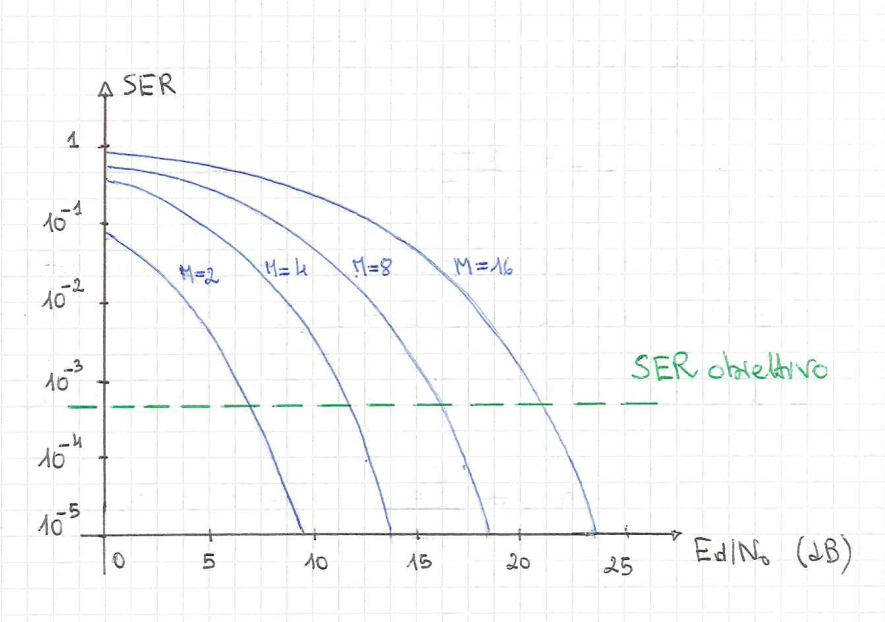
\includegraphics[width = 10cm]{media/scala_logaritmica_ser.png}
                    \caption{Scala logaritmica SER}
                \end{figure}
                La SER é espressa in scala logaritmica ed il rapporto $\frac{E_{simboli}}{N_0}$ é espresso in $db$.
                Viene solitamente fissata una probabilitá di errore obbiettivo stabilita in base all'applicazione, il
                rapporto $\frac{E_{simboli}}{N_0}$ richiesto per raggiungere la SER obbiettivo cresce al crescere della 
                cardinalitá $M$. Questo riduce come l'efficenza energetica del sistema diminuisca al crescere di $M$, entra piú rumore.
                Concludiamo che la scelta dell'alfabeto $\mathcal{A}$ é vincolata da due esigenze contrastanti:
                da un lato sarebbe bene scegliere una carinalitá $M$ elevata per aumentarne l'efficenza spettrale, dall'altro
                lato la scelta di un valore $M$ elevato peggiora l'efficenza energetica del sistema.
            \paragraph{Perdita Energetica: } Si definisce perdita energetica di un sistema di comunicazione numerico $A$ rispetto
                ad un sistema $B$ l'aumento (in $db$) del rapporto $\frac{E_{simboli}}{N_0}$ necessario al sistema $A$ per 
                raggiungere la stessa SER del sistema $B$. Un esempio mostrato in figura evince la perdita del sistema 
                4-PAM rispetto al sistema 2-PAM.
                \begin{figure}[H]
                    \centering
                    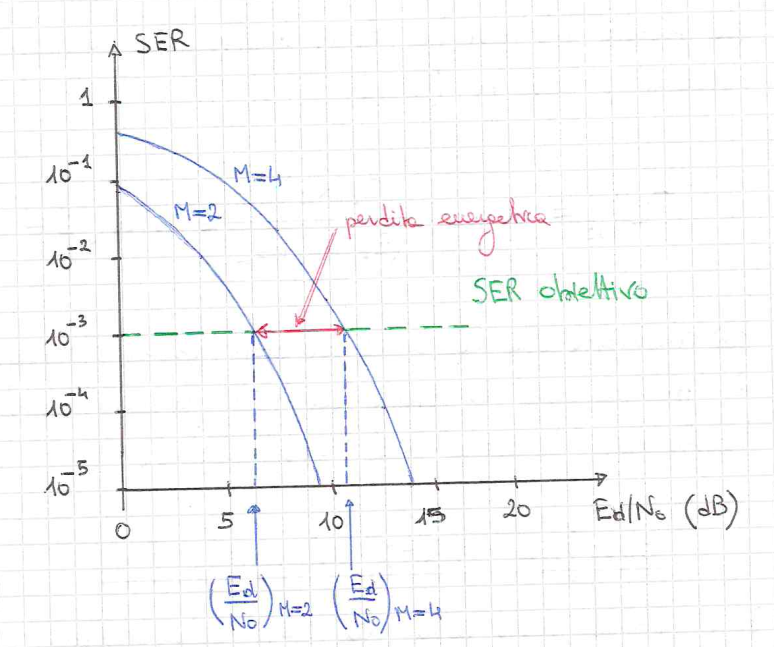
\includegraphics[width = 10cm]{media/comparazione errore ser.png}
                    \caption{differenza log 4PAM e 2PAM}
                \end{figure}  
                Calcoliamo la perdita in modo analitico basta eguagliare le SER della 4-PAM e della
                2-PAM ottenendo
                \[
                    \frac{3}{2}Q_{\displaystyle\left(\sqrt{\frac{4}{5}\left(\frac{E_s}{N_0}\right)_{M=4}}\right)} =Q_{\displaystyle\left(\sqrt{2\left(\frac{E_s}{N_0}\right)_{M=2}}\right)}      
                \]
                solitamente si tende a trascurare eventuali coefficienti moltiplicativi, potendo cosí confrontare direttamente
                l'argomento della funzione $Q$
                \[
                    \frac{4}{5}\left(\frac{E_s}{N_0}\right)_{M=4} =2\left(\frac{E_s}{N_0}\right)_{M=2}          
                \]
                la perdita del sistema 4-PAM rispetto al sistema 2-PAM é in $db$
                \[
                    \eval*{L}_{db} = 10log_{10}\left(\frac{\left(\frac{E_s}{N_0}\right)_{M=4}}{\left(\frac{E_s}{N_0}\right)_{M=2}}\right) = 10log_{10}\left(\frac{5}{2}\right) \simeq 4db    
                \]
                cioé comporta che la curva di SER per la 4-PAM é praticamente la stessa del sistema 2-PAM, salvo una traslazione di
                circa $4db$ verso destra.
            \paragraph{Esempio sistema 4-PAM}{

            }
        \subsubsection{Codifica GRAY nel sistema PAM}
            Abbiamo visto come la SER in un sistema PAM dipende dal rapporto $\frac{E_s}{N_0}$ e dalla cardinalitá 
            $M$ dell'alfabeto $\mathcal{A}$. Come sappiamo i simboli di modulazione $\{a_i\}$ in un sistema PAM sono
            il risultato della mappatura dei bit di codice $\{d_n\}$. Per l'utente finale sarebbe quindi piú utile 
            conoscere al posto della SER la probabilitá di errore sui bit $\{d_n\}$, chiamata Bit Error Rate (BER)
            \[
                BER = P_r[\hat{d}_n \neq d_n]    
            \] 
            in generale il calcolo della BER in un sistema PAM é un valore difficilmente calcolabile poiché oltre a dipendere
            dal rapporto $\frac{E_s}{N_0}$ e da $M$, dipende anche dalla legge di mappatura. É peró possibile 
            individuare facilmente un intervallo di valori entro quale siamo sicuri che si trovi la BER.
            Per individuare tale intervallo, supponiamo di utilizzare una trasmissione PAM usando un alfabeto
            M-ario e siano
            \begin{gather}
                N_s = \text{Numero di simboli trasmessi}\nonumber \\
                N_d = \text{Numero di bit trasmessi}\nonumber \\
                N_{se} = \text{Numero di simboli ricevuti errati}\nonumber \\
                N_{de} = \text{Numero di bit ricevuti errati}\nonumber 
            \end{gather}
            Si tenga presente che ogni simbolo PAM é ottenuto mappando un blocco di $log_2(M)$ bit, ho quindi
            \[
                N_d = N_slog_2(M)    
            \]
            inoltre ogni volta che un simbolo viene ricevuto con errore il numero dei corrispondenti bit sbagliati 
            varia da $1$ a $log_2(M)$. Si ha pertanto 
            \[
                N_{se} \leq N_{de} \leq N_{se} log_2(M)    
            \]
            dividendo i termini della precedente relazione per $N_d$ si trova
            \[
                \frac{N_{se}}{N_slog_2(M)} \leq \frac{N_{de}}{N_{d}} \leq \frac{N_{se} log_2(M)}{N_{s} log_2(M)}    
            \]
            e passando al limite per $N_s$ e $N_b$ tendendo all'infinito 
            \[
                \frac{SER}{log_2(M)} \leq BER \leq SER    
            \]
            da cui si vede che la BER non puó mai superare la SER. A seconda della legge di mappatura impiegata,
            la BER puó assumere valori piú vicini a $\frac{SER}{log_2(M)}$ o a SER. Vale la pena notare che la BER 
            coinciderebbe con il valore $\frac{SER}{log_2(M)}$ solo se, ogni volta che un simbolo ricevuto contiene 
            un errore, solo uno dei bit corrispondenti a quel simbolo é sbagliato. Questa osservazione é utile 
            per individuare quale sia la mappa ottima. Infatti, tenendo conto che quando un simbolo é ricevuto con errore
            molto probabilmente viene frainteso con un simbolo adiacente nell'alfabeto $\mathcal{A}$, la mappa ottima é 
            quella che associa a simboli adiacenti di $\mathcal{A}$ blocchi di $log_2(M)$ bit che differiscono per un solo bit. 
            Una tale mappa é nota come "Mappa GRAY", ed é quella che minimizza la BER per un prefissato valore della SER. 
            Se in un sistema PAM viene utilizzata la mappadi GRAY, la BER é espressa da 
            \[
                BER \simeq \frac{2(M-1)}{Mlog_2(M)}Q_{\displaystyle \left(\sqrt{\frac{6log_2(M)}{M^2-1}}\frac{E_d}{N_0}\right)}    
            \] 
    \subsection{QAM}
        É un sistema di comunicazione in {\color{red}banda passante} in cui il segnale trasmesso $s_{T(t)}$ ha densitá 
        spettrale di potenza di tipo passa-banda, centrate su una frequenza $f_0$ detta frequenza portante.
        \subsubsection{Inviluppo complesso}
            l'inviluppo complesso del segnale trasmesso é 
            \[
                \tilde{s}_{(t)} = I_{(t)} +j Q_{(t)}      
            \]
            e il segnale trasmesso
            \[
                  s_{T(t)} = \mathbb{R}e\{\tilde{s}_{(t)}e^{j\omega_0t}\}
            \]
            con $\omega_0 = 2\pi f_0$, $\tilde{s}_{(t)}\in \mathbb{C}$, $I_{(t)}\in \mathbb{R}$ detta parte in fase e 
            $Q_{(t)}\in \mathbb{R}$ detta parte in quadratura del segnale $s_{T(t)}$ il quale puó quindi essere espresso 
            come 
            \[
                s_{T(t)} =I_{(t)}\cos(\omega_0t)+jQ_{(t)}\sin(\omega_0t)  
            \]  
            e le singole parti possono essere espresse come 
            \begin{gather}
                I_{(t)} = \sum_{i}a_ig_{T(t-iT)}\nonumber \\
                Q_{(t)} = \sum_{i}b_ig_{T(t-iT)}\nonumber
            \end{gather}
            in cui $g_{T(t)}$ é l'impulso di trasmissione, $T$ é l'intervallo di segnalazione,
            $\{a_i\}$ e $\{b_i\}$ sono i simboli di modulazione, ottenuti dal mappaggio di bit del codice $\{d_n\}$.
            La mappa ha cardinalitá $M$ ed é di tipo bidimensionale, nel senso che ad ogni stringa di $log_2(M)$ bit di codice
            fa corrispondere una coppia $(a_i,b_i)$ disponibili nell'alafabeto impiegato. $M$ é il numero possibile di coppie $(a_i,b_i)$ 
            disponibili nell'alfabeto. Nel caso di mappe bidimensionali l'alfabeto é costituito da punti $(a_i,b_i)$ nel piano cartesiano,
            ed é detto \emph{costellazione}. Un esempio di costellazione quaternaria é mostrata nella figura seguente
            \begin{figure}[H]
                \centering
                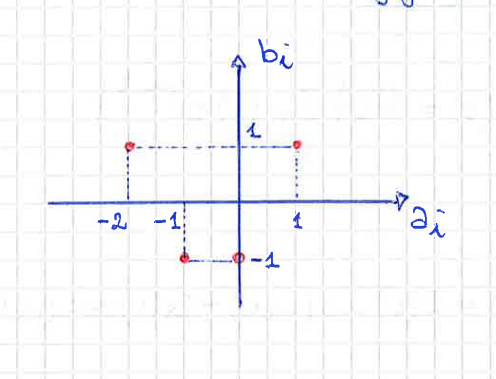
\includegraphics[width = 6.5cm]{media/costellazione quaternaria.png}
                \caption{Costellazione quaternaria}
            \end{figure}
        \subsubsection{Trasmettitore - QAM}
            Il trasmettitore usa un modulatore $I/Q$ come illustrato di seguito, dove $g_{T(t)}$ é un impulso a radice di coseno rialzato 
            come quello impiegato in un sistema PAM.
            \begin{figure}[H]
                \centering
                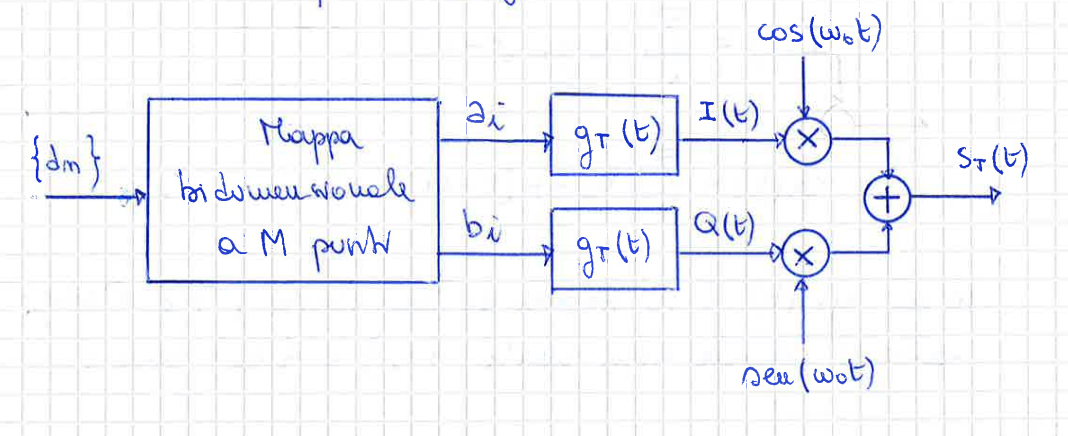
\includegraphics[width = 12cm]{media/trasmettitore qam.png}
                \caption{Trasmettitore QAM}
            \end{figure}
            L'inviluppo complesso del segnale trasmesso é espresso da
            \[
                \tilde{s}_{(t)} = I_{(t)} +jQ_{(t)} = \sum_{i}c_ig_{T(t-iT)}
            \]
            avendo definito i simboli complessi come 
            \[
                c_i = a_i+jb_i    
            \]
            e si vede che $\tilde{s}_{(t)}$ é in pratica un segnale PAM con simboli complessi. L'equivalente in banda base del trasmettitore é 
            \begin{figure}[H]
                \centering
                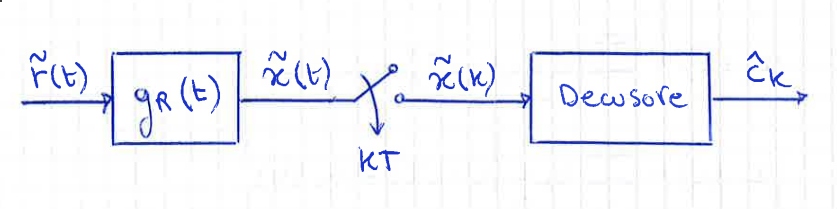
\includegraphics[width = 12cm]{media/equivalente ricevitore in banda base.png}
                \caption{Equivalente in Banda Base}
            \end{figure}
        \subsubsection{Densitá spettrale di potenza - QAM}
            Per il calcolo della densitá spettrale di potenza del segnale $s_{T(t)}$, si ricorda che essa é legata a quella dell'inviluppo
            complesso $\tilde{s}_{(t)}$ dalla relazione
            \[
                S_{s(f)} = \frac{1}{4}\left[S_{\tilde{s}{(f-f_0)}}+ S_{\tilde{s}{(-f-f_0)}}\right]    
            \]
            per cui é sufficiente calcolare la densitá spettrale di potenza $S_{\tilde{s}(f)}$. Ammettiamo che la sequenza dei 
            simboli $\{c_i\}$ sia stazionaria in senso lato con valore medio 
            \[
                \eta_c=\mathbb{E}[c_i]    
            \] 
            e funzione di autocorrelazione
            \[
                R_{c(m)} = \mathbb{E}[c_{i+m}c^\ast_i]    
            \]
            la densitá spettrale di potenza di $\tilde{s}_{T(t)}$ é la trasformata di Fourier di $R_{\tilde{s}{(f-f_0)}}$ ed é espressa da
            \[
                S_{\tilde{s}{(f)}} = \frac{1}{T} f_{c(f)}\left|G_{T(f)}\right|^2    
            \]
            dove 
            \[
                f_{c(f)} = \sum_{m}R_{c(m)}e^{-j2\pi fmT}
            \]
            é la densitá spettrale di potenza dei simboli complessi $\{c_i\}$. La potenza di $s_{T(t)}$ é quindi esprimibile come
            \[
                P_s=\frac{1}{2T} \int_{-\infty}^{\infty} f_{c(f)} \left|G_{T(f)}\right|^2 df
            \]
            Poiché $g_{T(t)}$ é un impulso tipicamente a radice di coseno rialzato, la banda di $\tilde{s}_{T(t)}$ é 
            \[
                B_{\tilde{s}}=\frac{1+\alpha}{2T}    
            \]
            la banda del segnale trasmesso $s_{T(t)}$ 
            \[
                B_{T}=2B_{\tilde{s}} =\frac{1+\alpha}{T}
            \]
            e l'efficenza spettrale del sistema risulta 
            \[
                \eta_{sp} = \frac{R_d}{B_T} = \frac{log_2(M)}{1+\alpha} 
            \]
            avendo tenuto conto che $R_d = \frac{log_2(M)}{T}$. Si osservi come l'efficenza spettrale del sistema aumenti all'aumentare 
            della cardinalitá $M$ della costellazione.
        \subsubsection{Ricevitore - QAM}
            Supponiamo che il canale sia non distorcente ed aggiunga solo rumore termico. In tale ipotesi, il segnale ricevuto 
            é espresso da
            \[
                r_{(t)} = s_{T(t)}+w_{(t)}    
            \]
            con $w_{(t)}$ rumore Gaussiano bianco avente densitá spettrale di potenza $\frac{N_0}{2}$. Il ricevitore ha la
            struttura mostrata in figura seguente 
            \begin{figure}[H]
                \centering
                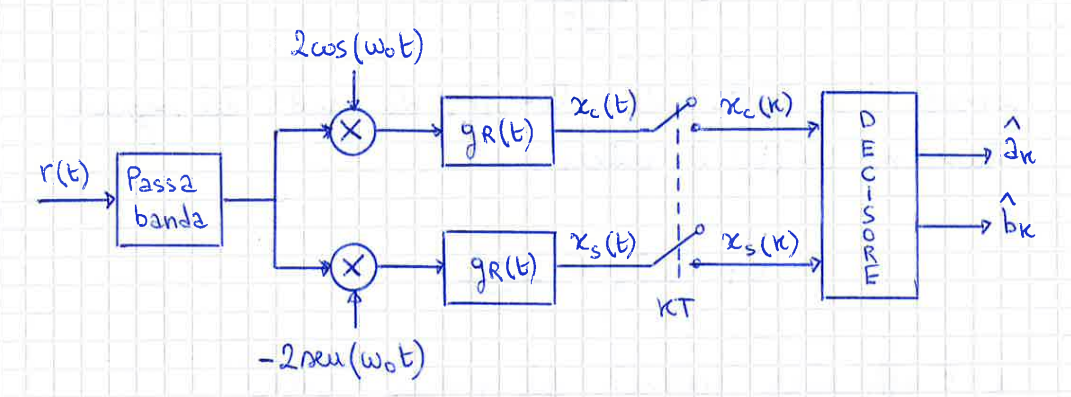
\includegraphics[width = 12cm]{media/ricevitore qam.png}
                \caption{Ricevitore QAM}
            \end{figure}            
            Il segnale ricevuto viene inviato a un filtro passa-banda(\ref{Filtro Passa Banda di banda B - Band Pass Filter (BP)})
            con frequenza centrale $f_0$ e tale da non distorcere il segnale utile. Esso serve a selezionare il segnale utile e ad 
            eleminare il rumore fuori banda. Dopo la demodulazione $I/Q$, il segnale passa attraverso il filtro di ricezione $g_{R(t)}$,
            tipicamente a radice di coseno rialzato, che sostituisce il passa-basso presente nel demodulatore di $I/Q$. I segnali 
            $x_{c(t)}$ e $x_{s(t)}$ in uscita dal filtro di ricezione sono espressi da 
            \begin{gather}
                x_{c(t)} = \sum_{i}a_ig_{(t-iT)}+n_{c(t)}\nonumber \\
                x_{s(t)} = \sum_{i}b_ig_{(t-iT)}+n_{s(t)}\nonumber
            \end{gather}
            dove $g_{(t)} = g_{(T(t))}\otimes g_{(R(t))}$ é un impulso a coseno rialzato, mentre $n_{c(t)}$ e $n_{s(t)}$ sono 
            processi di rumore Gaussiano, a media nulla e a densitá spettrale di potenza
            \[
                S_{n_c(f)} = S_{n_s(f)} = N_0\left|G_{R(f)}\right|^2   
            \]
            Qualora il filtro passa-banda sia simmetrico intorno a $f_0$ i processi $n_{c(t)}$ e $n_{s(t)}$ sono anche incorrelati, e quindi 
            indipendenti essendo congiuntamente Gaussiani. Dopo il campionatore abbimo i campioni $x_{c[k]}$ e $x_{s[k]}$ espressi da 
            \begin{gather}
                x_{c[k]} = a_{[k]}+n_{c[k]}\nonumber \\
                x_{s[k]} = b_{[k]}+n_{s[k]}\nonumber
            \end{gather}
            dove si é tenuto conto che $g_{(t)}$ sia un impulso di Nyquist. Le variabili aleatorie $n_{c[k]}$ e $n_{s[k]}$ sono 
            Gaussiane, a media nulla con varianza 
            \[
                \sigma^2 = N_0\int_{-\infty}^{\infty}\left|G_{R(f)}\right|^2df= N_0g_{RCR(0)} = N_0
            \]
            l'equivalente in banda base del ricevitore é 
            \begin{figure}[H]
                \centering
                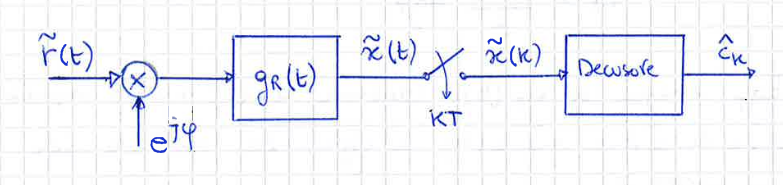
\includegraphics[width = 12cm]{media/equivalente in banda base ricevitore qam.png}
                \caption{Equivalente ricevitore in banda base}
            \end{figure}
            dove
            \begin{gather}
                \tilde{x}_{[k]} = c_{[k]}+\tilde{n}_{[k]} \nonumber \\
                \tilde{n}_{[k]} = n_{c[k]}+jn_{s[k]} \nonumber 
            \end{gather}
    \subsection{Modulazione Amplitude Shift Keyring - ASK}
        In questo tipo di modulazione, i simboli $b_i$ sono posti a zero, risolta quindi $Q_{(t)} = 0$. 
        Il segnale trasmesso risulta 
        \[
            s_{T(t)} = I_{(t)}\cos(\omega_0 t)
        \]
        dove $I_{(t)}$ é un segnale PAM
        \[
            I_{(t)} = \sum_{i}a_ig_{T(t-iT)}    
        \]
        con simboli $\{a_i\}$ appartenenti all'alfabeto M-ario $\mathcal{A} = \{\pm 1, \pm 3,\dots,\pm (M-1)\}$. Pertanto 
        il segnale ASK non é altro che un segnale PAM traslato in frequenza mediante modulazione classica. Lo schema trasmettitore 
        é riportato in figura 
        \begin{figure}[H]
            \centering
            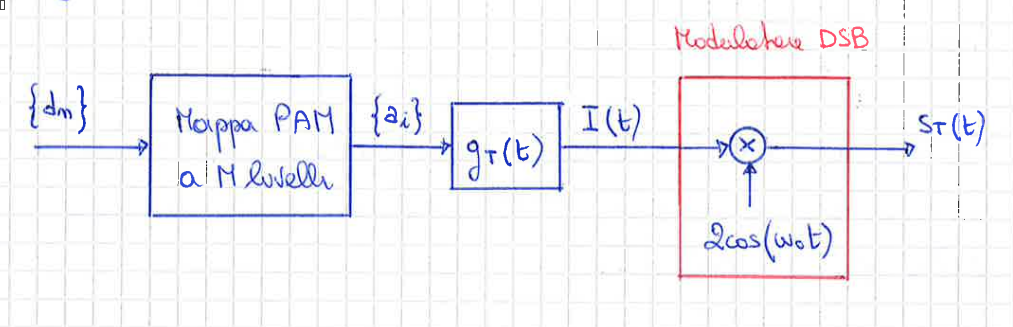
\includegraphics[width = 12cm]{media/trasmettitore ask.png}
            \caption{Trasmettitore ASK}
        \end{figure}        
        e si vede che é composto solo dal ramo relativo a $I_{(t)}$. Nel caso di simboli indipendenti ed equiprobabili, la densitá 
        spettrale di potenza dell'impulso complesso é 
        \[
            S_{\tilde{s}(f)} = \frac{M^2-1}{3T}\left|G_{T(f)}\right|^2
        \]
        e l'energia media per simbolo trasmesso é 
        \begin{align}
            E_s &= \frac{1}{2}T\int_{-\infty}^{\infty}S_{\tilde{s}(f)}df\nonumber \\
                &= \frac{M^2-1}{6}E_{g_T}\nonumber
        \end{align}
        essendo $E_{g_T}$ l'energia di $g_{T(t)}$. Qualora $g_{T(t)}$ sia un impulso a radice di coseno rialzato, l'efficenza spettrale
        del sistema ASK é 
        \[
            \eta_{sp} = \frac{log_2(M)}{1+\alpha}    
        \]
        ed é la metá di quella del corrispondente segnale PAM trasmesso in banda base. Il ricevitore é costituito da un demodulatore seguito da 
        un ricevitore per segnali PAM, secondo quanto riportato nella figura seguente
        \begin{figure}[H]
            \centering
            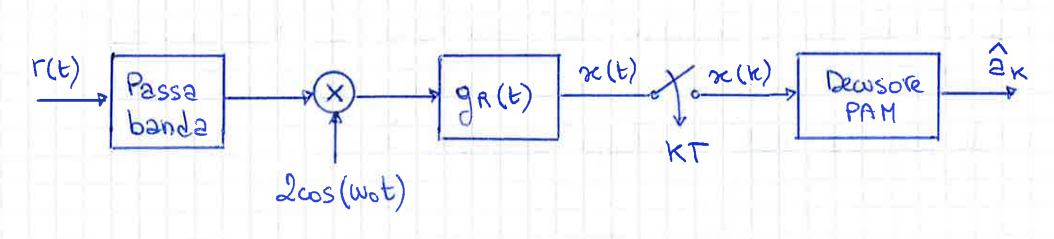
\includegraphics[width = 12cm]{media/ricevitore ask.png}
            \caption{Ricevitore ASK}
        \end{figure}
        Ricordando che il guadagno di demodulazione é pari a $1$, é facile capire che le prestazioni in termini di SER e BER per un sistema ASK
        M-ario coincidono con quelle di un sistema PAM. In particolare continua a valere che aumentando la cardinalitá $M$ dell'alfabeto 
        si ha una diminuzione dell'efficenza energetica a favore di un aumento in quella spettrale, a paritá di $M$ l'efficenza 
        spettrale del sistema ASK é la metá di quella del corrispondente sistema PAM. 
    \subsection{Modulazione Quadrature Amplitude Modulation - QAM}
        In questo tipo di modulazione, la cardinalitá $M$ della costellazione é una potenza di $4$, e i simboli $\{a_i\}$ e $\{b_i\}$
        vengono generati da due mappe PAM a $\sqrt{M}$ livelli che operano indipendentemente su bit diversi.
        \begin{figure}[H]
            \centering
            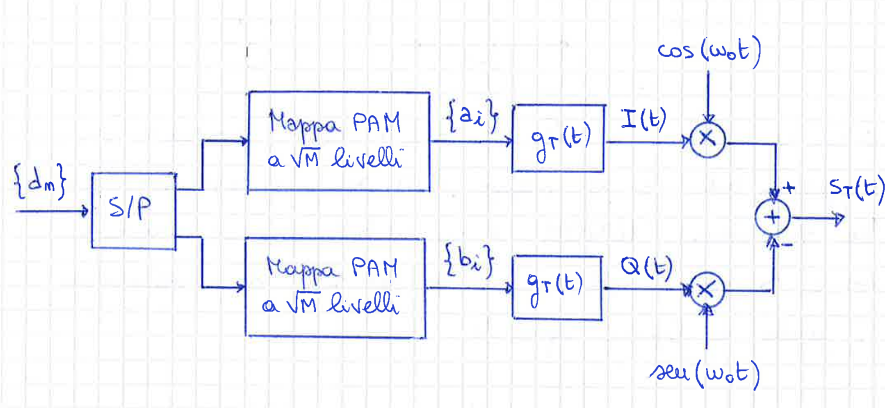
\includegraphics[width = 12cm]{media/modulatore qam.png}
            \caption{Modulatore QAM}
        \end{figure}
        \begin{sloppypar}
            come possiamo vedere in figura i bit $\{d_n\}$ entrano in un convertitore Serie/Parallelo ($S/P$) che divide il flusso in 
            due sottoflussi distinti. Ciascun sottoflusso entra in un mappatore PAM a $\sqrt{M}$ livelli con alfabeto
            ${\mathcal{A} = \{\pm 1, \pm 3,\dots, \pm(\sqrt{M}-1)\}}$ da cui escono i simboli $\{a_i\}$ e $\{b_i\}$, che vengono poi usati per generare 
            i segnali PAM $I_{(t)}$ e $Q_{(t)}$. Il segnale QAM equivale a una coppia di segnali PAM con simboli indipendenti trasmessi 
            contemporaneamente sul canale mediante due oscillazioni in quadratura. Nel caso di mappe PAM bianrie si ha un segnale 4-QAM aventi
            seguente costellazione
        \end{sloppypar}
        \begin{figure}[H]
            \centering
            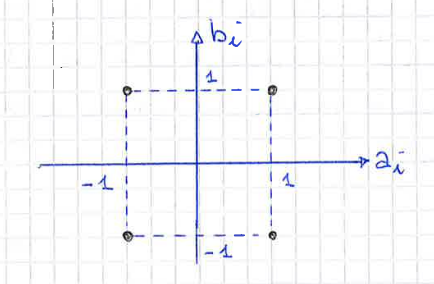
\includegraphics[width = 6.5cm]{media/costellazione qam.png}
            \caption{Costellazione QAM}
        \end{figure}
        in cui a ciascun simbolo $c_i = a_i +jb_i$ é associata una coppia di bit. Se le mappe PAM sono quaternarie si ha un sistema 
        16-QAM in cui 4 bit vengono mappati su di un simbolo complesso $c_i$, in tal caso la costellazione diventa la seguente
        \begin{figure}[H]
            \centering
            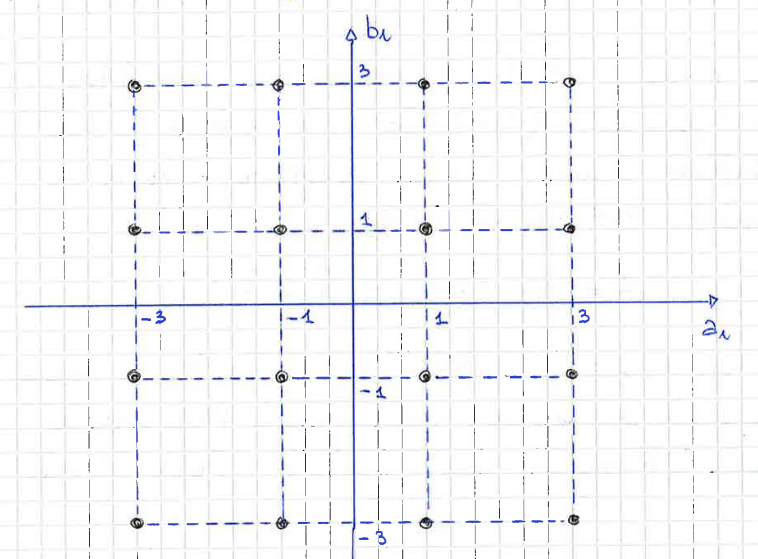
\includegraphics[width = 6.5cm]{media/costellazione 16qam.png}
            \caption{Costellazione 16-QAM}
        \end{figure}
        in caso di simboli indipendenti ed equiprobabili, la densitá spettrale di potenza dell'inviluppo complesso é 
        \[
            S_{\tilde{s}(f)} = \frac{C_2}{T}\left|G_{T(f)}\right|^2    
        \]
        dove 
        \[
            C_2 = \mathbb{E}[\left|c_i\right|^2] = \frac{2}{3}(M-1)    
        \]
        é la potenza media dei simboli trasmessi. Possiamo calcolare l'energia media per simbolo trasmesso
        \[
            E_s = \frac{1}{2}T\int_{-\infty}^{\infty}S_{\tilde{s}(f)} df = \frac{M-1}{3}E_{g_T}
        \]
        con $E_{g_T}$ energia di $g_{T(t)}$. Qualora $g_{T(t)}$ sia un impulso a radice di coseno rialzato, l'efficenza spettrale del 
        sistema QAM diventa 
        \[
            \eta_{sp} = \frac{log_2(M)}{1+\alpha}  
        \]
        ed é uguale a quella di ciascuno dei segnali PAM presenti sul ramo $I_{(t)}$ e sul ramo $Q_{(t)}$ del trasmettitore.
        Il ricevitore é costituito da un demodulatore $I/Q$ seguito da due ricevitori per segnali PAM
        \begin{figure}[H]
            \centering
            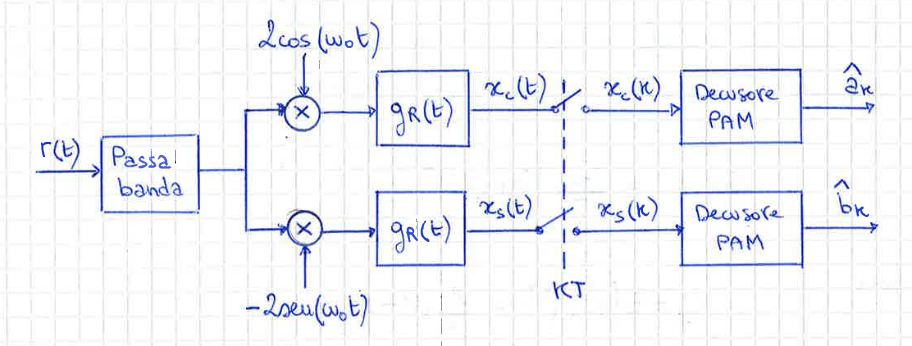
\includegraphics[width = 12cm]{media/ricevitore qam 2.png}
            \caption{Ricevitore QAM}
        \end{figure}
        Come possiamo vedere la decisione non é presa sul simbolo complesso $c_k$, ma sui simboli $a_k$ e $b_k$ in modo 
        indipendente mediante un decisore PAM a $\sqrt{M}$ livelli. Possiamo anche rappresentare il sistema nel suo
        equivalente in banda base nel caso sia presente un errore di fase $\phi$ durante la demodulazione $I/Q$
        \begin{figure}[H]
            \centering
            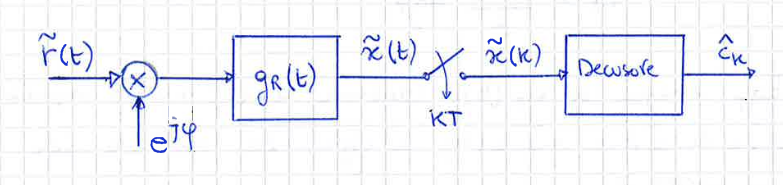
\includegraphics[width = 12cm]{media/equivalente in banda base ricevitore qam.png}
            \caption{Equivalente in banda base ricevitore QAM}
        \end{figure}
        In tal caso, assumendo l'assenza di ISI, il campione in uscita dal filtro di ricezione é 
        \[
            \tilde{x}_{[k]} = x_{c[k]}+ jx_{s[k]} = e^{j\phi}c_k+\tilde{n}_{[k]}  
        \]
        con le componenti 
        \begin{gather}
            x_{c[k]} = a_k cos(\phi) - b_k sin(\phi) + n_{c[k]}\nonumber \\
            x_{s[k]} = b_k cos(\phi) + a_k sin(\phi) + n_{s[k]}\nonumber
        \end{gather}
	    come si vede sul campione $x_{c[k]}$ é presente l'interferenza dovuta al simbolo $b_k$, mentre su $x_{x[k]}$ 
        é presente l'interferenza dovuta al simbolo $a_k$. É quindi necessario effettuare una buona sincronizzazione,  
        perché altrimenti sui campioni $x_{c[k]}$ e $x_{s[k]}$ avremo interferenza nonostante sia rispettata la condizione 
        di Nyquist per l'annullamento dell'ISI. L'errore di fase $\phi$ ha l'effetto di ruotare il campione ricevuto 
        $\tilde{x}_{[k]}$, con il rischio di portare $\tilde{x}_{[k]}$ fuori dalla zona di decisione relativa al simbolo 
        trasmesso. In figura mostra le zone di decisione per una 4-QAM e 16-QAM
        \begin{figure}[H]
            \centering
            \subfloat[4-QAM]{
                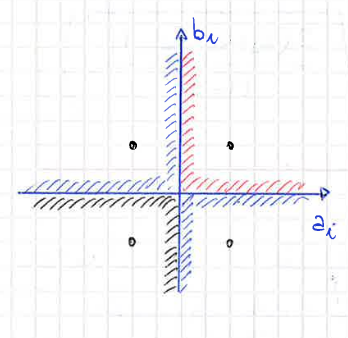
\includegraphics[width = 5cm]{media/4qam.png}
            }
            \hfill
            \subfloat[16-QAM]{
                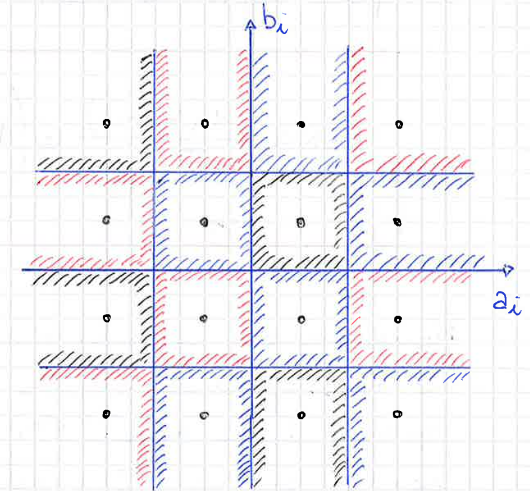
\includegraphics[width = 7cm]{media/16qam.png}
            }
        \end{figure}
        per quanto riguarda la costellazione 4-QAM, le zone di decisione sono i 4 quadranti del piano complesso, mentre
        la costellazione 16-QAM si ha una griglia di quadranti 4x4. La costellazione 16-QAM é piu sensibile all'errore 
        di fase rispetto alla costellazione 4-QAM. Per portare un simbolo fuori dalla propria zona di decisione 
        (in assenza di rumore) occorre una rotazione di $45^\circ$ per un sistema 4-QAM, mentre basta una rotazione di 
        meno di $20^\circ$ per un sistema 16-QAM.

        Nell'ipotesi di assenza di ISI e di perfetto sincronismo, le prestazioni di un sistema QAM in termini di BER 
        sono perfettamente analoghe a quelli di un sistema PAM a $\sqrt{M}$ livelli che costituiscono il segnale QAM.
        In presenza di codifica di GRAY, la BER é espressa approsimativamente da 
        \[
            BER \simeq \frac{4(\sqrt{M}-1)}{\sqrt{M}log_2(M)}Q_{\displaystyle \left(\sqrt{\frac{3log_2(M)}{M-1}\frac{E_d}{N_0}}\right)}  
        \]
        Possiamo pertanto concludere che il sistema QAM ha stessa efficenza energetica e stessa efficenza spettrale di due segnali PAM
        a $\sqrt{M}$ livelli che siano trasmessi sul ramo $I_{(t)}$ e $Q_{(t)}$. Rispetto al sistema ASK, ha la stessa efficenza energetica,
        ma efficenza spettrale doppia in quanto il segnale QAM é costituito da due segnali ASK modulati con frequenze portanti in 
        quadratura e trasmessi sulla stessa banda.

    \subsection{Modulazione Phase Shift Keyring - PSK}

        \subsubsection{Prestazioni di un sistema PSK}
    

    \section{Teoria Dei Codici}
    \subsection{Introduzione}
        Ci concentriamo adesso sul trattamento dell'informazione per poterla trasmettere.
        I messaggi che trasmettiamo possono essere codificati per vari motivi:
        \begin{itemize}
            \item {
                    Compressione:$\begin{cases}
                        \text{Lossy: con perdita dell'informazione} \nonumber\\
                        \text{Lossless: minima perdita dell'informazione} \nonumber
                    \end{cases}$\\
                    Comprimere l'informazione in elimenando ridondanza e salvando spazio di memoria e banda.
                    
                }
            \item {
                    Crittografia: per nascondere il messaggio ad utenti in ascolto sul canale che non siano il destinatario.
            }
            \item {
                    Rivelazione o correzione di errore: vieen aggiunta ridondanza ad hoc per aumentare l'affidabilitá del messaggio trasmesso. 
                    Si utilizzano \href{https://en.wikipedia.org/wiki/Checksum}{checksum} o \href{https://en.wikipedia.org/wiki/Reed-Solomon_error_correction}{Reed-Solomon(RS)}
            }
        \end{itemize}
        \paragraph{Capacitá del canale}\label{Capacita del canale}\index{Capacitá del canale}
            La capacitá del canale $C$ indica la massima quantitá d'informazione che puó essere trasmessain maniera affidabile su di un dato canale.
            La capacitá dipende dalla banda $B$ del canale e dal rapporto segnale rumore (signal-to-noise ratio,\href{https://en.wikipedia.org/wiki/Signal-to-noise_ratio}{$SNR$}):
            \[
                C = B\log(1 + SNR)  
            \] 
        \paragraph{Canale Gaussiano}\index{Canale Gaussiano}
            Il canale Gaussiano puó essere modellato come \href{https://en.wikipedia.org/wiki/Binary_symmetric_channel}{Binary Symmetric Channel (BSC)} con probabilitá di errore $p$. 
            Assumiamo gli errori tra loro indipendenti ($p_{(a,b)} = p_{(a)}\dotproduct p_{(b)}$):
        \begin{figure}[H]
            \centering
            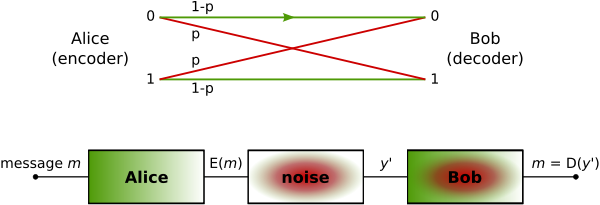
\includegraphics[width = 12cm]{media/600px-Binary_symmetric_channel_(en).svg.png}
            \label{BSC system}
            \caption{Sistema di trasmissione BSC}
        \end{figure}
        \begin{gather}
            E_{(x)}: \text{Funzione di codifica} \nonumber \\
            D_{(x)}: \text{Funzione di decodifica} \nonumber \\
            E_{(m)}: \text{Bit dell'informazione codificati} \nonumber \\
            y^\prime: E_{(m)}+ e \rightarrow \text{Informazioni con errore del canale} \nonumber \\
            m = D_{(y^\prime)}: \text{Informazione decodificata} \nonumber 
        \end{gather}
        Il canale é chiamato simmetrico perché ho la stessa probabilitá errore sulla trasmissione di uno dei due bit.
        Se $X$ é il bit inviato e Y quello ricevuto allora il canale é caratterizzato dalle probabilitá:
        \begin{align}
            P(Y=0|X=0) &= 1-p\nonumber \\
            P(Y=0|X=1) &= p\nonumber \\
            P(Y=1|X=0) &= p\nonumber \\
            P(Y=1|X=1) &= 1-p\nonumber 
        \end{align} 
        Assumiamo che $0\leq p \leq\frac{1}{2}$, se avessimo $p >\frac{1}{2}$ il ricevitore potrebbe scambiare l'informazione ricevuta
        (Quando riceve un $1$ lo interpreta come $0$ e viceversa) e ottenere un canale con probabilitá $1-p \leq\frac{1}{2}$. 
        
        Nel corso useremo delle simbologie diverse:
        \begin{figure}[H]
            \centering
            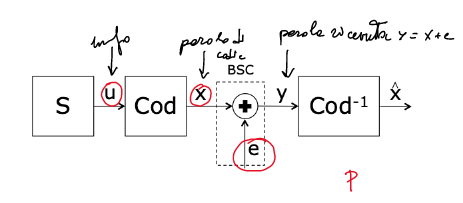
\includegraphics[width = 12cm]{media/BSC System.png}
            \label{BSC system moretti}
            \caption{Sistema di trasmissione BSC}
        \end{figure}
        \begin{gather}
            u: \text{Informazione} \nonumber \\
            x: \text{Parole di Codice} \nonumber \\
            e: \text{Errore del Canale} \nonumber \\
            y: x+e \rightarrow \text{Informazioni con errore del canale} \nonumber \\
            \overset{\wedge}{x}: \text{Informazione decodificata} \nonumber 
        \end{gather}
        \paragraph{Probabilitá di errore BSC}\label{Probabilita di errore BSC}\index{Probabilitá di errore BSC}
            La probabilitá, per una trasmissione BSC, di sbagliare $t$ bit in una parola di $n$ bit:
            \[
                p_{(t,n)} = \binom{n}{t} p^t (1-p)^{(n-t)}
            \]
            dove il coefficente binomiale:
            \[
                \binom{n}{t} = \frac{n!}{t!(n-t)!}
            \]
            indica tutte le possibili combinazioni di errori di $t$ bit su $n$ bit. 
        \paragraph{Tassonomia dei codici}
            \begin{itemize}
                \item {Codici lineari
                        \begin{itemize}
                            \item {
                                Codici a blocco
                                }
                            \item{
                                Codici convoluzionali
                            } 
                        \end{itemize}
                    }
                \item {
                    Definizione di un codice a blocco: 
                    \begin{figure}[H]
                        \centering 
                        \begin{tikzpicture}[
                            node distance=2cm,
                            >=latex
                            ]

                            \node [coordinate] (input) {};
                            \node [draw, rectangle,right of = input, minimum height=3em, minimum width=6em] (block) {$x_{(t)}$};
                            \node [coordinate, right of = block] (output) {};
                            
                            \draw[draw,->] (input) -- node[midway]{$/$} node[below]{$k$} (block);
                            \draw[->] (block) -- node[midway]{$/$} node[below]{$n$} (output);
                        \end{tikzpicture}    
                    \label{Def codice a blocco}
                    \end{figure}
                    \paragraph{Rate del Codice}:\index{Rate del Codice}
                        {
                            \[
                                R = \frac{k}{n}  
                            \]
                            La condizione é che $n>k$ senon fosse cosí avrei perdita d'informazione, da $k$ bit passo a $n$ aggiungendo
                            ridondanza e codificando i miei dati. Possiamo quindi stimare il valore tipico di $R$
                            \[
                                R = \frac{k}{n} <1  
                            \]
                        }
                }
                \item Rivelazione di errore:\index{Rivelazione di errore}{
                    Consiste nella capacità di scoprire la presenza di errori causati dal rumore o da altri fenomeni deterioranti 
                    durante una trasmissione di dati (es. tramite il \href{https://it.wikipedia.org/wiki/Bit_di_parit%C3%A0}{bit di paritá}).
                }
                \item {Correzione di errore:\index{Correzione di errore}{
                    Consiste invece nell'ulteriore abilità di ricostruire i dati originali, eliminando gli errori occorsi durante la trasmissione.
                    Vi sono due differenti schemi di base per la progettazione della codifica di canale e del protocollo per un sistema che corregge gli errori:
                    \begin{itemize}
                        \item {
                            ??\href{https://it.wikipedia.org/wiki/Automatic_repeat-request}{Automatic repeat-request} (ARQ): Il mittente invia i dati ed anche un codice a rilevazione d'errore, che sarà
                            utilizzato in ricezione per individuare gli eventuali errori, ed in tal caso chiedere la ritrasmissione dei dati
                            corrotti. In molti casi la richiesta è implicita; il destinatario invia un acknowledgement (ACK) di corretta 
                            ricezione dei dati, ed il mittente re-invia solo quei dati per i quali non ha ricevuto, entro un prefissato tempo 
                            limite (timeout), il corrispondente ACK.
                        }
                        \item{
                            ??\href{https://it.wikipedia.org/wiki/Forward_Error_Correction}{Forward Error Correction} (FEC): Il mittente codifica i dati con un codice a correzione d'errore 
                            (error correction code, ECC) ed invia il messaggio codificato. Il destinatario non invia mai alcun 
                            messaggio verso il mittente; esso decodifica ciò che riceve nella maniera più simile possibile a quella di un 
                            certo insieme prefissato di parole accettabili. Tali codici sono realizzati in modo tale che dovrebbe occorrere 
                            una quantità "irragionevole" di errori nei dati, affinché il destinatario decodifichi erroneamente, ottenendo 
                            finalmente dei dati diversi da quelli effettivamente inviatigli.
                        } 
                    \end{itemize}
                    In generale un codice a blocco che ha rate $\frac{k}{n}$ mappa $k$ bit su $n$ bit usando $2^k$ parole di codice di dimensione n
                }}
            \end{itemize}

        \subsubsection{Esempio codici a blocco: codici a ripetizione}
            É un esempio di codice a correzione d'errore: il funzionamento si basa sulal ripetizione dell'informazione piú volte. Il destinatario
            si accorge di un errore di trasmissione poiché il flusso di dati ricevuto non è la ripetizione di un singolo messaggio e, inoltre, 
            il destinatario può recuperare il messaggio originale guardando il messaggio ricevuto nel flusso di dati che si verifica più spesso.

            Nel caso di un codice binario di ripetizione, esistono due parole in codice - tutte uno e tutti zeri - che hanno una lunghezza n. 
            Pertanto, la distanza minima di Hamming (\ref{Distanza di Hamming}) del codice è uguale alla sua lunghezza. Ciò conferisce al codice 
            di ripetizione, con $R = \frac{1}{n}$,una capacità di rivelazione di errori pari a $n-1$ e correzione degli errori (cioè correggerà fino agli errori in qualsiasi parola del codice) di $\frac{n-1}{2}$ per n dispari(\ref{Probabilita di errore BSC}).\\
            Esempio:\\
            \indent{$R = \frac{1}{3} \rightarrow$ ha solo 2 parole di codice:}
            \begin{align}
                u=0 \rightarrow x = [000]\nonumber \\
                u=1 \rightarrow x = [111]\nonumber
            \end{align} 
            Il ricevitore effettua una decodifica a maggioranza: decide per il bit che comprare piú volte della parola ricevuta.
            \begin{align}
                y = [000] \rightarrow \overset{\wedge}{x} = [000] \rightarrow \overset{\wedge}{u} = 0 \nonumber \\
                y = [010] \rightarrow \overset{\wedge}{x} = [000] \rightarrow \overset{\wedge}{u} = 0 \nonumber \\
                y = [101] \rightarrow \overset{\wedge}{x} = [111] \rightarrow \overset{\wedge}{u} = 1 \nonumber
            \end{align}
            \paragraph{Evento errore:} l'evento errore per un codice a correzione di errore consiste nel non essere in grado di correggere
            tutti gli errori introdotti dal canale. Se la probabilitá di errore sul bit $p_{e,b}$ é piccola, la probabilitá di errore 
            $p_{e,W}$ per il codice puó essere approssimata dal primo evento che determina la ricezione errata (nel caso dei codici a ripetizione a $R = \frac{1}{3}$ 
            si verifichino $2$ errori).
            \begin{itemize}
                \item {$R = \frac{1}{3}$
                    \begin{itemize}
                        \item {
                            Se $p_{e,b} = 0.1 \Rightarrow p_{e,W} \approx 2.7\dotproduct 10^{-2} $ 
                        }
                        \item {
                            Se $p_{e,b} = 0.01 \Rightarrow p_{e,W} \approx 2.97\dotproduct 10^{-4} $ 
                        }
                    \end{itemize}
                }
                \item {$R = \frac{1}{5}$
                    \begin{itemize}
                        \item {
                            Se $p_{e,b} = 0.1 \Rightarrow p_{e,W} \approx 8.1\dotproduct 10^{-3} $ 
                        }
                        \item {
                            Se $p_{e,b} = 0.01 \Rightarrow p_{e,W} \approx 9.8\dotproduct 10^{-6} $, Sviluppiamo i calcoli come esempio: 
                            \[
                                P_r \{\text{codice }R=\frac{1}{5}\text{ non riesce a correggere gli errori introdotti dal canale}\}:
                            \]
                            \begin{align}
                                P_r &= \sum_{t=3}^{5} \binom{5}{t}p^t (1-p)^{5-t},\hspace{0.2cm} p=10^{-2} \nonumber \\
                                P_r &\{\text{3 errori su 5}\}= \binom{5}{3}p^3 (1-p)^{5-3} = 10\dotproduct 10^{-6} (0.99)^2 = 9.8\dotproduct 10^{-6} \nonumber \\
                                P_r &\{\text{3 errori su 5}\}= \binom{5}{4}p^4 (1-p)^{5-4} = 5\dotproduct 10^{-8} (0.99) = 5\dotproduct 10^{-8}\nonumber \\
                                P_r &\{\text{3 errori su 5}\}= \binom{5}{5}p^5 (1-p)^{5-5} = 1\dotproduct 10^{-10} = 10^{-10}\nonumber 
                            \end{align}
                        }
                    \end{itemize}
                }
            \end{itemize}

        \subsubsection{Esempio codici a blocco: codici a controllo di paritá}
        Il bit di parità è un codice di controllo d'errore, utilizzato nei calcolatori per prevenire errori nella trasmissione o nella memorizzazione dei dati. 
        Tale codice prevede l'aggiunta di un bit ridondante ai dati, calcolato a seconda che il numero di bit che valgono 1 sia pari o dispari. Ne esistono
        quindi 2 varitá: bit di paritá pari e bit di paritá dispari. Quando si usa il bit di paritá pari si aggiunge un bit con valore $1$ se nella parola inviata
        il numero di occorrenze di "$1$" é dispari(portando il numero di occorrenze di "$1$" a una quantitá pari).Quando si usa il bit di paritá dispari si
        aggiunge un bit con valore $1$ se nella parola inviata il numero di occorrenze di "$1$" é pari (portando il numero di occorrenze di "$1$" a una quantitá dispari).

        \noindent Il codice ha $R = \frac{k}{(k+1)}$: $k$ bit informativi piú il bit di paritá.
        
        \paragraph{Rilevazione dell'errore:}La rilevazione d'errore deriva dalla discordanza del numero di occorrenze di "$1$", eseguendo lo XOR bit a bit, nel caso del bit di paritá pari, se il risultato
        é $0$ non sono avvenuti errori, viceversa se ho un risultato uguale a $1$ posso dire che cé stato uno o una quantitá dispari di errori nella trasmissione, questo lo rende
        solo un codice a rilevazione d'errore e non un codice a correzione d'errore.
        
        Esempio:Trasmetto parole di $11bit$ con rate $R_b = 10Mb/s$ e probabilitá di errore sul bit trasmesso $p_{e,b} = 10^{-8}$:
        \begin{itemize}
            \item {
                Senza controllo di paritá é sufficiente che sia sbagliato anche un solo bit per sbagliare tutta la parola:
                \[
                    p_{e,W} = \sum_{j=1}^{11} \binom{11}{j}p_{e,b}^j (1-p_{e,b})^{11-j} = 11 p_{e,b} (1-p_{e,b})^{10} \simeq 11p_{e,b}
                \]
                ed il rate di parole sbagliate al secondo é:
                \[
                    R_{e,W} = \frac{R_b}{11}\dotproduct p_{e,W} \simeq \frac{10^7}{11}\dotproduct 11p_{e,b} = 0.1_\frac{w}{s}
                \]
            }
            \item {
                Aggiungendo un bit di paritá, la parola diventa di 12 bit e sbaglio quando faccio almeno 2 errori, il singolo errore
                viene corretto chiedendo nuovamente la trasmissione del dato:
                \[
                    p_{e,W} = \sum_{j=2}^{12} \binom{12}{j}p_{e,b}^j (1-p_{e,b})^{12-j} = 66 p_{e,b}^2 (1-p_{e,b})^{10} \simeq 66p_{e,b}^2
                \]
                ed il rate (frequenza) di parole sbagliate al secondo é:
                \[
                    R_{e,W} = \frac{R_b}{12}\dotproduct p_{e,W} \simeq \frac{10^7}{12}\dotproduct 66p_{e,b}^2 = 5.5\dotproduct 10^{-9} \frac{w}{s}
                \]
                possiamo anche calcolare il periodo $T_{e,W} = \frac{1}{R_{e,W}} =  1.82\dotproduct 10^{8} s$ che é una parola ogni sei anni circa.  
            }
        \end{itemize}
        \subsubsection{Esempio codici a blocco: codice ISBN}
            Il codice International Standard Book Number (ISBN) é un codice a controllo di paritá per un alfabeto di simboli nonbinari. 
            Ad ogni libro é assegnata una parola di codice di lunghezza $n=10$ cifre in base decimale. Le prime 9 cifre identificano il libro, 
            la decima é quella di controllo di paritá cosí calcolata:
            \begin{enumerate}
                \item {
                    Si calcola la grandezza $z = mod(S,11)$ con
                    \[
                        S = \sum_{j=1}^{9} (11-j)x_{(j)}
                    \]
                }
                \item {
                    La cifra di controllo di aritá é il complemento a 11 di $z$:
                    \[
                        x_{(10)} = mod(11-z,11)  
                    \]
                    E solo per la cifra di controllo di paritá se $x_{(10)} = 10$ si sostituisce con 
                    $x_{(10)} = X$
                }
            \end{enumerate}
            Quando un dispositivo legge il codice lo verifica come segue:
            \begin{enumerate}
                \item {
                    Moltiplica ogni cifra per il peso della posizione della stessa cifra e calcola $mod(S^\prime,11)$ con
                    \[
                        S^\prime = \sum_{j=1}^{10} (11-j)y_{(j)}
                    \]
                }
                \item {
                    Assumendo che non ci siano errori su $x_{(10)} = |11-z|_{11}$, si ha:
                    \begin{align}
                        mod(S^\prime,11) &= mod \left( \sum_{j=1}^{9} (11-j)y_{(j)} + mod(11-z,11),11\right) \nonumber \\
                                         &= mod \left( \sum_{j=1}^{9} (11-j)y_{(j)} + \left(11-\sum_{j=1}^{9} (11-j)x_{(j)}\right),11\right)\nonumber \\
                                         &= mod \left(\sum_{j=1}^{9} (11-j)(y_{(j)}-x_{(j)}),11\right)
                    \end{align}
                }
            \end{enumerate}
            Se non ci sono errori si ha $y=x$ e quindi il $mod(S^\prime,11) = 0$
            \paragraph{Rivalazione degli errori:} Il codice é in grado di rivelare tutti i singoli errori:
            sia $e_{(k)}$ l'errore in posizione $k$,$y_{(k)} = x_{(k)}+ e_{(k)}$:
            \[
                mod(S^\prime,11) = mod((y_{(k)}-x_{(k)})(11-k),11)+mod(e_{(k)}(11-k),11) \neq 0
            \]
            Il codice é in grado di rivelare tutti i casi in cui ci sia uno scambio di 2 cifre del codice. Siano 
            $k_1$ e $k_2$ le 2 posizioni scambiate:
            \begin{align}
                mod(S^\prime,11) &= mod \left((y_{(k_1)}-x_{(k_1)})(11-k_1)+(y_{(k_2)}-x_{(k_2)})(11-k_2),11\right) \nonumber \\
                                 &= mod \left((x_{(k_2)}-x_{(k_1)})(11-k_1)+(x_{(k_1)}-x_{(k_2)})(11-k_2),11\right)\nonumber \\
                                 &= mod \left((x_{(k_2)}-x_{(k_1)})(k_2-k_1),11\right) \neq 0 \nonumber
            \end{align}
            Esempi:
            \begin{itemize}
                \item {Senza errore:
                    \begin{align}
                        ISBN & = 01-333-5485-7 \nonumber \\
                        \left| S^\prime \right|_{11} &= 0\dotproduct 10 +1\dotproduct 9+3\dotproduct 8+3\dotproduct 7+3\dotproduct 6+5\dotproduct 5+4\dotproduct 4+8\dotproduct 3+5\dotproduct 2+7\dotproduct 1\nonumber \\
                        \left| S^\prime \right|_{11} &= \left| 154 \right|_{11} = 0 \nonumber 
                    \end{align}
                    Il codice é corretto 
                }
                \item {Con errore: Scambio le cifre
                    \begin{align}
                        ISBN & = 01-333-5458-7 \nonumber \\
                        \left| S^\prime \right|_{11} &= 0\dotproduct 10 +1\dotproduct 9+3\dotproduct 8+3\dotproduct 7+3\dotproduct 6+5\dotproduct 5+4\dotproduct 4+{\color{red}5\dotproduct 3}+{\color{red}8\dotproduct 2}+7\dotproduct 1\nonumber \\
                        \left| S^\prime \right|_{11} &= \left| 151 \right|_{11} = 8 \neq 0 \nonumber 
                    \end{align}
                    Il codice non é corretto 
                }
            \end{itemize}
        \subsection{Codici a blocco}
        \subsubsection{Introduzione ai codici lineari}
            \paragraph{Campo:} un campo é una struttura composta da un insieme non vuoto $F$ e da due operazioni binarie interne: $\forall \alpha,\beta,\gamma \in F$:
                \begin{itemize}
                    \item {
                        Somma ($XOR$):
                        \begin{itemize}
                            \item {
                                \[
                                    \alpha + \beta = \theta, \theta \in F  
                                \]
                            }
                            \item {Associativa:
                                \[
                                    (\alpha + \beta) + \gamma = \alpha +( \beta + \gamma)
                                \]
                            }
                            \item {Commutativa:
                                \[
                                    \alpha + \beta = \beta + \alpha
                                \]
                            }
                            \item {Elemento Neutro:
                                \[
                                    0\in F,\alpha + 0 = \alpha,\alpha-\alpha = 0
                                \]
                            }
                        \end{itemize}
                    }
                    \item {
                        Prodotto ($AND$):   
                        \begin{itemize}
                            \item {
                                \[
                                    \alpha \dotproduct \beta = \theta, \theta \in F  
                                \]
                            }
                            \item {Associativa:
                                \[
                                    (\alpha \dotproduct \beta) \dotproduct \gamma = \alpha \dotproduct( \beta \dotproduct \gamma)
                                \]
                            }
                            \item {Commutativa:
                                \[
                                    \alpha \dotproduct \beta = \beta \dotproduct \alpha
                                \]
                            }
                            \item {Distributiva:
                                \[
                                    (\alpha + \beta) \dotproduct \gamma = \alpha \dotproduct \gamma + \beta \dotproduct \gamma
                                \]
                            }
                            \item {Elemento Neutro:
                                \[
                                    1\in F,\alpha \dotproduct 1 = \alpha,\forall \alpha \neq 0\rightarrow \alpha\dotproduct\alpha^{-1} = 0
                                \]
                            }
                        \end{itemize}
                    }
                \end{itemize}
        \subsubsection{Campi di Galois}
            Un campo finito, detto anche campo di Galois, é un campo con un numero finito $q$ di elementi. Il numero di elementi di definisce la categoria del
            campo: $GF(2)$ é il campo definito su $\{0,1\}$ con somma modulo 2 ($XOR$) e prodotto modulo 2 ($AND$). Definito lo spazio $GF(2)$ si puó costruire
             lo spazio vettoriale $\mathcal{V}_n=GF(2)^2$, lo spazio di tutti i possibili $2^n$ vettori di $n$ cifre binarie su cui valgono le operazioni definite per 
             $GF(2)$.

        \subsubsection{Codici a blocco lineari su $GF(2)$}
            Sia $u = [u_1, \dots, u_k]$ una generica parola di $k$ cifre binarie. Il codice a blocco lineare $\mathcal{C}(k,n)\subset \mathcal{V}_n$ é l'insieme delle
            $2^k$ parole $x = [x_1, \dots, x_n]$ di $n$ cifre binarie ottenute con la trasformazione lineare:
            \[
                x = uG  
            \]
            Dove $G$ é la matrice generatrice del codice e ha dimensione $k \times n$ di cifre binarie con $n>k$ poiché al massimo
            aggiungo informazioni per la trasmissione, per la correzione o rivelazione d'errore.
            
            Siano $g_i, i = [1, \dots, k]$, le righe di $G$, $x$ é la combinazione lineare delle righe $g_i$:
            \[
                x = \sum_{i=1}^{k}u_ig_i  
            \]
            Per avere $2^k$ parole di codice distinte  é necessario che $G$ abbia rango $k$: le righe di $G$ devono essere linearmente indipendenti e costituiscono 
            una $base$ per il sottospazio vettoriale $\mathcal{C} \subset \mathcal{V}_n$.  

        \subsubsection{Propietá dei codici a blocco lineari}
            Le propietá derivano maggiormente dalla pripietá di linearit;a dei codici:
            \begin{itemize}
                \item {Ogni parola di codice é una combinazione lineare di righe della matrice generatrice.}
                \item {Il codice a blocchi é costituito da tutte le possibili combinazioni delle righe della matrice generatrice.}
                \item {La somma di due parle di codice é ancora una parola di codice.}
                \item {La $n-upla$ di tutti zeri é sempre una parola di codice.}
                \item {Se $x$ é una parola di codice, anche $-x$ é una parol di codice.}
            \end{itemize}

        \subsubsection{Distanza di Hamming}\label{Distanza di Hamming}\index{Distanza di Hamming}
            La distanza di Hamming tra due vettori, o stringhe, $d(x_1,x_2)$ di $n$ elementi é il nuemro di posizioni in cui le due parole
            sono diverse tra loro. Esempi:
            \begin{itemize}
                \item {
                    La distanza di Hamming tra 10{\color{red}1}1{\color{red}1}01 e 10{\color{red}0}1{\color{red}0}01 è 2.
                }
                \item {
                    La distanza di Hamming tra 2{\color{red}14}3{\color{red}8}96 e 2{\color{red}23}3{\color{red}7}96 è 3.
                }
            \end{itemize}
            \paragraph{Peso di Hamming:}\label{Peso di Hamming}\index{Peso di Hamming} Il peso di Hamming,$w(x)$, di una stringa i lunghezza $n$ é la sua distanza di Hamming dal vettore di $n$ zeri,
            $x_0\in \mathcal{V}_n$ é:
            \[
                w(x_0) = d(x_0,0_n)
            \]
            \paragraph{Distanza minima:}\label{Distanza minima}\index{Distanza minima}La distanza minima di un codice $\mathcal{C}$ é la minima distanza di Hamming calcolata fra tutte le possibili parole che appartengono a $\mathcal{C}$.
            \[
                d_{min} (\mathcal{C})= \underset{x_1,x_2 \in \mathcal{C}}{min}d(x_1,x_2)  
            \]
            Per i codici lineari vale che ciascuna parola di codice ha lo stesso insieme di distanze dalle altre parole di codice.
            La distanza minima di un codice si puó calcolare a partire da qualsiasi parola di codice. 
            La distanza di Hamming é una metrica:
            \begin{itemize}
                \item {}
                \item {}
                \item {}
                \item {}
            \end{itemize}
        \subsubsection{Codici a blocco in forma sistematica}
            Quando il codice é in forma sistematica la matrice generatrice del codice ha la seguente forma:
            \begin{gather}
                G = [I_k,P]\nonumber \\
                G\in k\times n,\ I\in k\times k,\ P\in k\times (n-k)\nonumber
            \end{gather}
            dove la matrice $P$ é la matrice di paritá, il suo contenuto dipende da quale algoritmo di paritá viene scelto.
            \begin{figure}[H]
                \centering 
                \begin{tikzpicture}[
                    node distance=2cm,
                    >=latex
                    ]

                    \node [coordinate] (input) {};
                    \node [draw, rectangle,right of = input, minimum height=3em, minimum width=6em] (block) {Coder};
                    \node [coordinate, right of = block] (output) {};
                    
                    \draw[draw,->] (input) -- node[midway]{$/$} node[below]{$k$} (block);
                    \draw[->] (block) -- node[midway]{$/$} node[below]{$n$} (output);
                \end{tikzpicture}    
            \label{Def codice forma sistematica}
            \end{figure}
            \begin{figure}[H]
                \centering 
                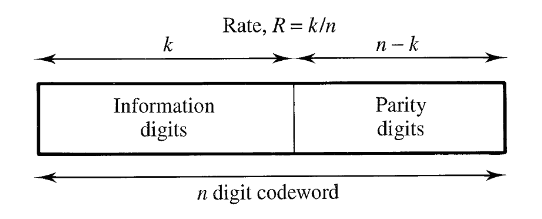
\includegraphics[width = 8cm]{media/forma sistematica.png}
            \label{matrice forma sistematica}
            \end{figure}
            \paragraph{Esempio Codice a ripetizione:}
            $R = \frac{1}{3},\ k=1,\ n=3$
            \begin{table}[H]
                \centering
                \begin{tabular}{|c|c|}
                \hline
                Bit i  ingresso & Parola codificata \\ \hline
                0               & {[}000{]}         \\ \hline
                1               & {[}111{]}         \\ \hline
                \end{tabular}
            \end{table}
            La matrice generatirce del codice é $G = [111]$, e la distanza minima $d_{min} = 3$\\

            \paragraph{Esempio Codice a controllo di paritá:}
            $R = \frac{7}{8},\ k=7,\ n=8$, ogni 7 bit ne aggiunge uno di controllo di paritá, 1 se il numero di "1" é diapari,
            0 se il numero di "1" é diapari.


            \noindent La matrice generatirce del codice:
            \[
                G = [I_7,1_7]
            \]
            \noindent La distanza minima é $d_{min} = 2$, se cambio uno dei 7 bit della parola
            cambio automaticamente il bit di paritá, quindi cambiare 1 bit in realtá ne cambia 2.\\

            \noindent Il prodotto $u\dotproduct 1_7 = \sum_{i=1}^{7}u_i$, puó essere scritto come una soma modulo 2, vale 0 se il numero di 
            occorrenze di "1" é pari e 1 altrimenti. Non facciamo altro che calcolare il bit di paritá della parola $u$.
            
            \paragraph{Definizione:} Due codici lineari $\mathcal{C}_1(k,n)$ e $\mathcal{C}_2(k,n)$ in $GF(2)$ sono equivalenti se uno é ottenuto dall'altro
            attraverso una permutazione delle posizioni del codice.

            \paragraph{Teorema:} Due matrici generatrici $G_1$ e $G_1$ in $GF(2)$ generano due codici equivalenti se una puó essere ottenuta dall'altra
            da una sequenza di operazioni come:
            \begin{itemize}
                \item Permutazione delle righe.
                \item Combinazione lineare delle righe.
                \item Permutazione delle colonne.
            \end{itemize}
            
            \paragraph{Teorema:} Qualsiasi codice lineare a blocchi é equivalente ad un codice in forma sistematica.

            \paragraph{Propietá degli spazi:}
            \begin{itemize}
                \item {
                    Dato il sottospazio $\mathcal{C} \subset \mathcal{V}_n$ di dimensione $k$, esiste un sottospazio ortogonale (null space)
                    $\mathcal{C}^\perp \subset \mathcal{V}_n$ di dimensione $n-k$ definito da una matrice $H\in (n-k) \times n$:
                    \[
                        GH^T = 0_{n-k}  
                    \]
                }
                \item {
                    La base di $\mathcal{C}^\perp$ é costituita dalle $n-k$ righe della matrice $H$, per cui ogni elemento $t\in \mathcal{C}^\perp$ puó 
                    essere rappresentato:
                    \[
                        t = vH = \sum_{i=1}^{n-k}v_ih_i  
                    \]
                }
                \item {
                    Per ogni $x\in \mathcal{C}$ e per ogni $t\in \mathcal{C}^\perp$ si ha:
                    \[
                        xt^T = uGH^Tv^T = 0
                    \]  
                }
            \end{itemize}
        \subsubsection{Matrice di controllo di paritá}\label{Matrice di controllo di parita}\index{Matrice di controllo di paritá}
            La matrice $H$ é la matrice di controllo di paritá del codice. Per costruzione $\forall x \in \mathcal{C}$ vale:
            \begin{gather}
                    xH^T = uGH^T = 0 \nonumber \\
                    H\in (n-k) \times n\nonumber 
            \end{gather}
            La matrice $H$ non é unica, ma se il codice é sistematico posso ricavarla in un'altra forma:
            \begin{gather}
                H = [P^T,I_{n-k}] = 0 \nonumber \\
                H\in (n-k) \times n,\ I\in (n-k)\times (n-k),\ P^T\in (n-k) \times k \nonumber
            \end{gather}
            Se fosse $\neq 0$ ció che é stato ricevuto non é una parola di codice.
            
            \paragraph{Esempio codice a ripetizione e controllo di paritá:}
                $R = \frac{1}{3},\ k=1,\ n=3,\ n-k=2$ ho la matrice a controllo di paritá:
                \[
                    H= [P^T,I_2] =
                        \begin{bmatrix}
                        1 & 1 & 0\\
                        1 & 0 & 1
                        \end{bmatrix}  
                \]  
                Per un codice con $R = \frac{7}{8},\ k=7,\ n=8,\ n-k=1$ la matrice a controllo di paritá:
                \[
                    H= [P^T,I_1] = 1_8^T
                \]
        \subsubsection{Propietá dei codici a blocco}
            \paragraph{Teorema:} La distanza minima del codice a blocco $\mathcal{C}(k,n)$ si puó calcolare come il 
            peso di Hamming minimo tra tutte le parole di codice:
            \begin{align}
                d_{min}(\mathcal{C}) &= \underset{x_i,x_j\in\mathcal{C}}{\min} d_H(x_i,x_j) = \underset{x_i,x_j\in\mathcal{C}}{\min} d_H(x_i+x_j,x_j+x_j)\nonumber \\
                                     &= \underset{x_i,x_j\in\mathcal{C}}{\min} d_H(x_i+x_j,0_{1,n}) \overset{[x_i+x_j\in\mathcal{C}]}{\Rightarrow} \underset{x_i\in\mathcal{C}}{\min}\ w(x_i)\nonumber
            \end{align}
            \paragraph{Capacitá di rivelare errori (Error Detection):}
                Su un canale $BSC$ senza memoria (\ref{BSC system moretti}), la $n-upla\ y$ a valle del decisore puó essere rappresentata:
                \[
                    y=x+e  
                \] 
                Dove $e$ é il vettore di errori introdotto dal canale, se il canale non introduce errori: $e = 0_{1,n}$
                Sia $x$ la parola di codice trasmessa e $y=x+e$ la corrispondente sequenza di $n$ bit ricevuta. supponiamo che il canale 
                introduca un numero di errori:$w(e) > 0$, si dice:
                \begin{itemize}
                    \item {
                        Errore Rivelabile\index{Errore Rivelabile}: se $y$ non é una parola di codice, $y\notin\mathcal{C}(k,n) $
                    }
                    \item {
                        Errore Non Rivelabile\index{Errore Non Rivelabile}: se $y$ é una parola di codice ma non quella trasmessa, $w(e) \geq d_{min}$ 
                    }
                \end{itemize} 
                \subparagraph{Teorema:} Il codice $\mathcal{C}(k,n)$ é in grado di rivelare con certezza fino a $d_{min}-1$ errori.
                \begin{itemize}
                    \item {
                        Se $d(x,y)<d_{min}$: $y$ non puó essere una parola di codice, altrimenti vorrebbe dire cge esistono due parole di codice la cui distanza 
                        é minore di $d_{min}$.
                    }
                    \item {
                        Se $d(x,y)=d_{min}$: esiste almeno una parola di codice $c\in\mathcal{C}(k,n),\ c \neq x$ tale che $d(x,c)=d_{min}$, se $y=c$ l'errore non 
                        puó essere rivelato. 
                    }
                \end{itemize}
            \paragraph{Strategia di decodifica a massima verosomiglianza:}
                Sia $y$ il vettore ricevuto a seguito della trasmissione su $BSC$ , la strategia di decodifica a massima verosomiglianza (ML, maximum likelihood) 
                consiste nel trovare il vettore $\hat{x}$ che, tra tutte le $2^k$ possibili parole di codice $x$, massimizza la probabilitá condizionata 
                $P(y|x)$:
                \[
                    \hat{x} = \arg \underset{x\in\mathcal{C}}{\max}\ P(y|x)
                \]
                Poiché gli eventi di errore sono indipendenti da bit a bit, posso riscrivere la probabilitá condizionata come il prodotto delle probabilitá condizionate
                ottenute per ciascun bit trasmesso:
                \[
                    P(y|x) = \prod_{\ell=1}^{n} P(y_\ell|x_\ell)
                \]
                Lavorando in $GF(2)$ la probabilitá $P(y_\ell|x_\ell)$ puó assumere solo 2 valori:
                \[
                    P(y_\ell|x_\ell) = 
                    \begin{cases}
                        1-p &se\ P(y_\ell =x_\ell|x_\ell)\nonumber \\    
                        p   &se\ P(y_\ell \neq x_\ell|x_\ell)\nonumber     
                    \end{cases}
                \] 
                Osservazione: La distanza di Hamming $d_H(x,y)$ misura il numero di posizione diverse tra $x$ e $y$, quindi $n-d_H(x,y)$ minura il numero di posizioni
                uguali tra $x$ e $y$.

                La probabilitá $P(y|x)$ si calcola:
                \[
                    P(y|x) = p^{d_H(x,y)}(1-p)^{n-d_H(x,y)} =(1-p)^{n}\left(\frac{p}{1-p}\right)^{d_H(x,y)} 
                \]
                Mi interessa scegliere un $x$ che massimizza $\left(\frac{p}{1-p}\right)^{d_H(x,y)}$, é un valore $<1$:
                \begin{itemize}
                    \item {
                        Se ho la $d_H(x,y)$ piccola ho la probabilitá minore di errore.
                    }
                    \item {
                        Se ho la $d_H(x,y)$ alta ho la probabilitá di errore alta.
                    }
                \end{itemize}
                
            \paragraph{Decisione a massima verosomiglianza:}\label{Decisione a massima verosomiglianza}\index{Decisione a massima verosomiglianza}
                La parola di codice decisa $\hat{x}$ é quella che minimizza la distanza dalla parola $y$ ricevuta:
                \[
                    \hat{x} = \arg \underset{x\in\mathcal{C}}{\max}\ P(y|x) = \arg \underset{x\in\mathcal{C}}{\min}\ d_H(y,x)
                \]
                Scelgo $x$ tale che mi dia la minima distanza
                \subparagraph{Ricevitore ML ottimo:}\index{Ricevitore ML ottimo} Il ricevitore ML ottimo é il ricevitore a distanza minima, il ricevitore
                che associa alla sequenza di $n$ bit ricevuta $y$, la parola di codice $x$ che minimizza la $d_H(y,x)$.
                \subparagraph{Ricevitore ML error correction:}\index{Ricevitore ML error correction} Il ricevitore ML é in grado di correggere cn successo tutti quegli errori
                $e$ per cui la parola ricevuta $y = x+e$ é comunque piú vicina alla parola trasmessa $x$ che a qualsiasi altra parola del codice.
                
                Per ogni vettore $v\in\mathcal{V}_n$ e un reggio $r$ esiste una "sfera" di raggio $r$ i cui elementi sono tutti quei vettori in $\mathcal{V}_n$ che hanno
                distanza di Hamming da $v$ minore o uguale a $r$

                \begin{figure}[H]
                    \centering 
                    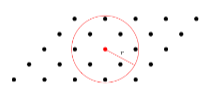
\includegraphics[width = 4cm]{media/sfera di amming.png}
                \label{sfera di Hamming}
                \end{figure}
                Se adottiamo un ricevitore ML, il numero massimo di errori che il codice $\mathcal{C}(k,n)$ é in grado di correggere é il massimo raggio $t$ per cui le sfere centrate nelle 
                parole di codice di $\mathcal{C}(k,n)$ sono tutte tra loro disgiunte.
            \paragraph{Capacitá di correggere errori (Error Correction):}
                \subparagraph{Teorema:}\begin{sloppypar}
                   Un codice lineare a blocco puó correggere fino a ${t_{max} = \left\lfloor \frac{d_{min}-1}{2} \right\rfloor}$ errori: $2t_{max}+1 \leq d_{min} \leq 2t_{max}+2$.
                \end{sloppypar}
                    
                \begin{sloppypar}
                    La condizione per cui le sfere di raggio $t$ che circondano le parole di codice siano disgiunte é che ${2t_{max} < d_{min}\Rightarrow t_{max} < \frac{d_min}{2}}$.
                    Altrimenti se fosse  ${2t_{max} \geq d_{min}}$ ci sarebbero almeno die parole $x_1$ e $x_2$ la cui distanza ${d_H(x_1,x_2) = d_{min} < 2t_{max} }$ e le que sfere di raggio
                    $t$ avrebbero almno un unto in comune.
                \end{sloppypar}
                
                \begin{sloppypar}
                    Consideriamo il codice $\mathcal{C}(k,n)$ che ha una certa $d_{min}$ e $t_{max}$ tale che ${2t_{max}+1 \leq d_{min}}$. Sia $x\in\mathcal{C}(k,n)$ la parola trasmessa,
                    ${y = x+e}$ la corrispondente sequenza di $n$ bit ricevuta e $c\in\mathcal{C}(k,n)$ un'altra generica parola di codice. Grazie alla disuguaglianza triangolare ho:
                    \[
                        d_H(x,y) + d_H(c,y) \geq d_H(x,c) \Rightarrow d_H(c,y) \leq d_H(x,c) - d_H(x,y)  
                    \]
                    per ipotesi ho anche:
                    \[
                        d_H(x,c) \geq d_{min} \geq 2t_{max}+1 
                    \]
                    Supponiamo che il canale introduca un certo numero di errori ${t\leq} t_{max}$, cosí da avere $d_H(x,y) = t$:
                    \[
                        d_H(c,y) \geq 2t_{max}+1 -t > t_{max} \geq t = d_H(x,y)   
                    \]   
                \end{sloppypar}
                
    \subsection{Codici di Hamming}
        I codici di Hamming $\mathcal{C}_H(m)$ sono definiti a partire da un parametro: $m \geq 2$
        \[
            n = 2^m-1,\ k = 2^m-m-1 = n-m
        \]
        \subparagraph{Matrice di controllo di paritá:} per definizione la matrice $H \in (n-k)\times n$, ma per i codici di Hamming la matrice $H$ ha dimensione:
        $H \in m\times (2^m-1)$.

        \subparagraph{Matrice di paritá:} Per un codice di Hamming sistematico la matrice di parità $P\in k \times m$ viene costruita cosí che le colonne di $H = [P^T,I_{n-k}]$
        siano tutte le possibili $2^m-1$ combinazioni di $m$ bit (esclusa la $n-upla$ di tutti 0)

        \subsubsection{Il codice $\mathcal{C}_H(2)$}
            \begin{sloppypar}
                Il codice a ripetizione ${R=\frac{1}{3}}$ con ${m=2\Rightarrow n=3,\ k=1}$ ha come matrice di controllo di paritá $H$:
                \[
                    H = \begin{bmatrix}
                            1  & 1 & 0 \\
                            1  & 0 & 1 \\
                        \end{bmatrix} 
                \]
                Che é la matrice corrispondente a un codice di Hamming $\mathcal{C}_H(2)$, poiché rappresenta tutte le possibili combinazioni di 2 bit
            \end{sloppypar}

        \subsubsection{Il codice $\mathcal{C}_H(3)$}
        \begin{gather}
            m=3,\ n=7,\ k=4,\ R=\frac{4}{7} \nonumber \\
            H = \begin{bmatrix}
                1 & 0 & 1 & 0 & 1 & 0 & 1\\
                0 & 1 & 1 & 0 & 0 & 1 & 1\\
                0 & 0 & 0 & 1 & 1 & 1 & 1
            \end{bmatrix}  \nonumber
        \end{gather}
        Posso ricavare la matrice generatrice $G$ scrivendo la matrice $H$ come se l'avessi ottenuta da una matrice $G\in k \times n$ di un codice sistematico (\ref{Matrice di controllo di parita}):
        \[
            H = [P^T,I_{n-k}] =\begin{bmatrix}
                                 1  & 1 & 0 & 1 & | & 1  & 0 & 0\\
                                 1  & 0 & 1 & 1 & | & 0  & 1 & 0\\
                                 0  & 1 & 1 & 1 & | & 0  & 0 & 1
                            \end{bmatrix} 
        \]
        La cui matrice generatrice con $I \in k \times k$ é:
        \[
            G = [I_{k},P] =\begin{bmatrix}
                                 1  & 0 & 0 & 0 & | & 1  & 1 & 0\\
                                 0  & 1 & 0 & 0 & | & 1  & 0 & 1\\
                                 0  & 0 & 1 & 0 & | & 0  & 1 & 1\\
                                 0  & 0 & 0 & 1 & | & 1  & 1 & 1
                            \end{bmatrix} 
        \]
        Possiamo vedere come la matrice di paritá faccia conrolli su combinazioni diverse di bit in ingresso $p = uP$:
        \begin{gather}
            p_1 = u_1+u_2+u_4 \nonumber\\
            p_2 = u_1+u_3+u_4 \nonumber\\
            p_3 = u_2+u_3+u_4 \nonumber
        \end{gather}
        Il vettore di uscita dal codificatore sará quindi $x = uG = [u,p_1,p_2,p_3]$, tale matrice di paritá ci permette di aumentare la distanza di Hamming
        tra le parole
        \subparagraph{Distanza minima:} La distanza minima di un qualsiasi codice di Hamming $\mathcal{C}_H(m)$ é $d_{min}(\mathcal{C}_H(m)) = 3$.

        \noindent Dimostrazione: 
        \begin{enumerate}
            \item {
                $d_{min} = \underset{x\in\mathcal{C}}{\min}\ w(x)$  
            }
            \item {
                $x\in\mathcal{C}\ se\ xH^T= 0$ e le colonne di $H$ sono tutte le possibili combinazioni dei bit $m$ bit
            }
        \end{enumerate}
        Perché $3$ é il numero minimo di colonne che mi permette di ottenere $0$ ($2$), quindi $d_{min}(\mathcal{C}_H(m)) = 3$.
        
        %Ne consegue che aumentando il numero di bit trasmessi diminuisco la ridondanza, ma la mia distanza di Hamming rimane sempre la stessa.
    \subsection{Decodifica per codici a blocco}
        Dato il vettore ricevuto:
        \[
            y = x+e
        \]
        Il decisore ottimo selezione la parola di codice $\hat{x}$:
        \[
            \hat{x} = \arg \underset{x\in\mathcal{C}}{\max}\ P(y|x) = \arg \underset{x\in\mathcal{C}}{\min}\ d_H(y,x)   
        \]
        Per ottenere $\hat{x}$ é necessario fare $2^k$ confronti tra il vettore ricevuto $y$ e tutte le parole di codice $\mathcal{C}(k,n)$, 
        la complessitá cresce esponenzialmente con $k$.

        Un approccio alternativo é quello di osservare il vettore errore e la probabilitá condizionata:
        \begin{gather}
            y= x+e \Rightarrow x = y+e,\ e = y-x\nonumber\\
            P(x|y) = P(x+e|x) = P(e|y+e\in\mathcal{C})\nonumber
        \end{gather}
        Posso ottenera la stima di $x$ come:
        \[
            \hat{x} = \arg \underset{x\in\mathcal{C}}{\max}\ P(y|x) =y+ \arg \underset{e}{\max}\ P(e|y+e\in\mathcal{C})   
        \]
        Invece di stimare $\hat{x}$ si stima il vettore $\hat{e}$ piú probabile
        \begin{align}
            \hat{e} &= \arg \underset{e}{\max}\ P(e|y+e\in\mathcal{C}) = \arg \underset{e|y+e\in\mathcal{C}}{\max}\ p^{w(e)}(1-p)^{n-w(e)} \nonumber \\
                    &= \arg \underset{e|y+e\in\mathcal{C}}{\max}\ \left(\frac{1-p}{p}\right)^{-w(e)} = \arg \underset{e|y+e\in\mathcal{C}}{\min}\ w(e)  \nonumber 
        \end{align}
        La decodifica sceglie tra tutti i possibili vettori errore $e$ tali che $y+e\in\mathcal{C}$ quello che ha il peso di Hamming minimo, cioé il minimo numero di 
        errori (Massima Verosomiglianza). Una volta stimato $\hat{e}$:
        \[
            \hat{x} = y-\hat{e} = y+\hat{e} = x+(\hat{e}+e)=
            \begin{cases}
                x &se\ \hat{e} = e\nonumber\\    
                x_1\neq x &se\ \hat{e} \neq e\nonumber    
            \end{cases}     
        \]
        \subsubsection{Coset}
            Sia $\mathcal{C}(k,n)$ un codice a blocco e sia $v\in \mathcal{V}_n$ un vettore di $n$ cifre binarie, si definisce $coset$ di
            $\mathcal{C}(k,n)$ individuato da $v$ l'insieme:
            \[
                C_v = C+v=\{ x+v: x\in\mathcal{C} \}
            \]
        \subsubsection{Propietá dei coset}
            \begin{enumerate}
                \item {Qualsiasi vettore in $\mathcal{V}_n$ appartiene a un coset di $\mathcal{C}(k,n)$}
                \item {Ciascun coset contiene $2^k$ elementi}
                \item {Due coset o sono coincidenti o hanno intersezione nulla}
                \item {Ci sono $2^{n-k}$ coset distinti}
                \item {Se $v_1$ e $v_2$ appartengono all ostesso coset, $v_1 + v_2 \in \mathcal{C}(k,n)$ é una parola di codice}
            \end{enumerate}
            \paragraph{Esempio di coset:}
                \begin{sloppypar}
                    Sia ${\mathcal{C}(2,3) = \{000,101,010,111\}}$. I coset di ${\mathcal{C}(2,3)}$: 
                \end{sloppypar}
                \begin{align}
                    \mathcal{C} + 000 = \{000,101,010,111\} = \mathcal{C}_0 \\
                    \mathcal{C} + 001 = \{001,100,011,110\} = \mathcal{C}_1 \\
                    \mathcal{C} + 010 = \{010,111,000,101\} = \mathcal{C}_0 \\
                    \mathcal{C} + 011 = \{011,110,001,100\} = \mathcal{C}_1 \\
                    \mathcal{C} + 100 = \{100,001,110,011\} = \mathcal{C}_1 \\
                    \mathcal{C} + 101 = \{101,000,111,010\} = \mathcal{C}_0 \\
                    \mathcal{C} + 110 = \{110,011,100,001\} = \mathcal{C}_1 \\
                    \mathcal{C} + 111 = \{111,010,101,000\} = \mathcal{C}_0 
                \end{align}
                Il numero di coset é $2^{n-k} = 2^{3-2} =2$.

            Si possono applicare i coset per la decodifica: $y=x+e$ dalla definizione di coset discende che i vettori $e$ e $y$
            appartengono allo stesso coset $\mathcal{C}_y$ e che i coset $\mathcal{C}_e$ e $\mathcal{C}_x$ sono coincidenti. Grazie alla propietá
            dei coset la somma di qualsiasi elemento di $\mathcal{C}_y$ con $y$ individua una parola di codice. Il vettore $e$ va scelto fre gli elementi
            di $\mathcal{C}_y$, la regola di decisione diveta:
            \[
                \hat{e} = \arg \underset{e}{\max}\ P(e|y+e\in\mathcal{C}) = \arg \underset{e\in\mathcal{C}_y }{\max}\ P(e) =\arg \underset{v\in\mathcal{C}_y }{\max}\ w(v)
            \] 
            Tra tutti i $2^k$ possibili vettori di $\mathcal{C}_y$, il principio di massima verosomiglianza dice che devo scegliere quello di peso minimo.
        \subsubsection{Algoritmo di decodifica}
            \begin{enumerate}
                \item Avendo ricevuto il vettore $y$ si trova un coset di appartenenza $\mathcal{C}_y$.
                \item {Si identifica il coset leader, la parola di peso minimo del coset $\mathcal{C}_y$, che é anche la parola di peso minimo del 
                coset di $\mathcal{C}_e$.}
                \item Il coset leader é la stima del vettore di errore $\hat{e}$
            \end{enumerate}
            \paragraph{Esempio di decodifica utilizzando i coset:}
                    Sia ${\mathcal{C}(2,4) = \{0000,1011,0101,1110\}}$ con $d_{min} = 2$, ho i coset: 
                \begin{align}
                    \mathcal{C} + 0000 = \{0000,1011,0101,1110\} \\
                    \mathcal{C} + 0001 = \{0001,1010,0100,1111\} \\
                    \mathcal{C} + 0010 = \{0010,1001,0111,1100\} \\
                    \mathcal{C} + 1000 = \{1000,0011,1101,0110\} 
                \end{align}
                Il numero di coset é $2^{n-k} = 2^{4-2} =4$. Il coset (2) non so quale coset leader scegliere hanno lo stesso peso di Hamming, ci
                troviamo in questo poiché la $d_{min}$ é molto bassa e ho il $50\%$ di possibilitá di sbagliare se il codice ricevuto capita in questo coset.
                Decodifichiamo:
                \begin{itemize}
                    \item {$y=[1101]\Rightarrow y\in (4),\text{coset leader:} [1000]\ \hat{x}=y+1000=0101$}
                    \item {$y=[1111]\Rightarrow y\in (2),\text{coset leader:} [0001] \vee [0100] \ \hat{x}=y+0001=1110$}
                \end{itemize}
        \subsubsection{Decodifica mediante sindrome}
            Si definisce sindrome di $y$ il vettore $s$ ottenuto dal prodotto di $y$ con la matrice di controllo di paritá:
            \[
                s = yH^T = (x+e)H^T = xH^T+eH^T = eH^T    
            \]
            \paragraph{Propietá:}
                \begin{itemize}
                    \item {
                        Tutti i membri di uno stesso coset hanno la stessa sindrome
                    }
                    \item {
                        $s \in 1 \times (n-k)$
                    }
                    \item {
                        Le $2^{n-k}$ sindromi sono associate ai $2^n-k$ diversi coset del codice $\mathcal{C}(k,n)$
                    }
                    \item {
                        Ciascuna sindrome é associata ai $2^k$ pattern di errore apparteenti allo stesso coset.
                    }
                \end{itemize}
            \paragraph{Procedura di decodifica:}
                \begin{enumerate}
                    \item {Calcola la sindrome $s = yH^T$}
                    \item {Associa la sindrome al coset leader corrispondente $s\rightarrow e_{CL}(s)$}
                    \item {Corregge l'errore sommando il coset leader alla $n-upla\ y$}
                \end{enumerate}
                La parola $\hat{x}$ é una parola di codice:
                \[
                    \hat{x}H^T= (y+e_{CL}(s))H^T = s+s =0   
                \]
                e per costruzione la parola di codice $\hat{x}$ minimizza la distanza di Hamming da $y$
        \subsubsection{Decodifica a sindrome: Codici di Hamming $m=3$}
            \begin{sloppypar}
                Il codice ha $d_{min} = 3$ ed é in grado di correggere esattamente un errore: ${t_{max} = \left\lfloor \frac{d_{min}-1}{2}\right\rfloor = 1}$. Si sceglie la matrice $H$
                in maniera che la tabella di decodifica associ alla sindrome il pattern di errore a peso 1 in cui il bit
                messo a 1 sia nella posizione corrispondente alla conversione della sindrome in decimale.
            \end{sloppypar}
            \begin{table}[H]
                \subfloat[Codice non sistematico]{
                    \begin{tabular}{cc}
                        \hline
                        Sindrome  & Coset Leader  \\ \hline
                        {[}000{]} & {[}0000000{]} \\
                        {[}100{]} & {[}1000000{]} \\
                        {[}010{]} & {[}0100000{]} \\
                        {[}110{]} & {[}0010000{]} \\
                        {[}001{]} & {[}0001000{]} \\
                        {[}101{]} & {[}0000100{]} \\
                        {[}011{]} & {[}0000010{]} \\
                        {[}111{]} & {[}0000001{]} \\ \hline
                        \end{tabular}
                }
                \hfill
                \subfloat[Codice sistematico]{
                    \begin{tabular}{cc}
                        \hline
                        Sindrome  & Coset Leader  \\ \hline
                        {[}000{]} & {[}0000000{]} \\
                        {[}100{]} & {[}0000100{]} \\
                        {[}010{]} & {[}0000010{]} \\
                        {[}110{]} & {[}1000000{]} \\
                        {[}001{]} & {[}0000001{]} \\
                        {[}101{]} & {[}0100000{]} \\
                        {[}011{]} & {[}0010000{]} \\
                        {[}111{]} & {[}0001000{]} \\ \hline
                    \end{tabular}
                }
            \end{table}
        \subsubsection{Esempio di decodifica}
            Un codice lineare a blocchi ha la seguente matrice di controllo di parità:
            \[
                H=
                    \begin{bmatrix}
                    1 & 0 & 1 & 1 & 0 & 0\\
                    1 & 1 & 0 & 0 & 1 & 0\\
                    0 & 1 & 1 & 0 & 0 & 1
                    \end{bmatrix}  
            \]  
            \begin{enumerate}
                \item {Determinare la matrice generatrice:
                    \begin{itemize}
                        \item{ 
                            Ci accorgiamo che il codice é in forma sistematica: abbiamo la matrice identica 
                            \[
                                H=
                                    \begin{bmatrix}
                                    1 & 0 & 1 & | & 1 & 0 & 0\\
                                    1 & 1 & 0 & | & 0 & 1 & 0\\
                                    0 & 1 & 1 & | & 0 & 0 & 1
                                    \end{bmatrix}  
                            \]  
                            Allora la forma $H = [P^T,I_{n-k}]$, e la matrice paritá ha forma $G = [I_k,P]$:
                            \[
                                G=
                                    \begin{bmatrix}
                                    1 & 0 & 0 & | & 1 & 1 & 0 \\
                                    0 & 1 & 0 & | & 0 & 1 & 1 \\
                                    0 & 0 & 1 & | & 1 & 0 & 1 
                                    \end{bmatrix}  
                            \]
                        }
                    \end{itemize}
                }
                \item {Decodificare la parola $y = [110110]$ ed identificare la parola di codice trasmessa:
                    \begin{itemize}
                        \item {Verifichiamo se é stato introdotto errore, calcoliamo la sindrome $s = yH^T$ e calcoliamone il prodotto in $G(2)$:
                        \[
                            yH^T=
                                \begin{bmatrix}
                                1 & 1 & 0 & 1 & 1 & 0
                                \end{bmatrix}
                                \begin{bmatrix}
                                1 & 1 & 0 \\ 
                                0 & 1 & 1 \\ 
                                1 & 0 & 1 \\ 
                                1 & 0 & 0 \\
                                0 & 1 & 0 \\
                                0 & 0 & 1 
                                \end{bmatrix} =
                                    \begin{bmatrix}
                                    0 & 1 & 1 
                                    \end{bmatrix}   
                        \]
                        }
                        \item {Essendo il codice diverso da $0$ é stato introdotto un errore, devo trovare la stima dell'errore: $y=x+e$ sia una parola di codice. 
                            La sindrome identifica un coset e di conseguenza l'errore a esso associato. Ma mi accorgo che $[011]$ (sindrome) corrisponde a una riga della matrice di controllo di paritá $H$, quindi posso solezionare la riga moltiplicandola per un vettore 
                            riga composto da zeri tranne un uno per la riga che voglio selezionare (questo avrá peso 1):
                            
                            \begin{align}
                                    \hat{x} &= y + \hat{e} =  (y + \hat{e})H^T=y H^T+ \hat{e}H^T= s+s =0 \nonumber \\
                                    &\begin{bmatrix}
                                        0 & 1 & 0 & 0 & 0 & 0
                                        \end{bmatrix}
                                        \begin{bmatrix}
                                        1 & 1 & 0 \\ 
                                        0 & 1 & 1 \\ 
                                        1 & 0 & 1 \\ 
                                        1 & 0 & 0 \\
                                        0 & 1 & 0 \\
                                        0 & 0 & 1 
                                        \end{bmatrix} = 0  \nonumber
                            \end{align}  
                        }
                        \item {Abbiamo quindi 
                        \begin{gather}
                            \hat{y} =\begin{bmatrix}
                                1 & 1 & 0 & 1 & 1 & 0
                                \end{bmatrix} \nonumber \\
                            \hat{e} = \begin{bmatrix}
                                0 & 1 & 0 & 0 & 0 & 0
                                \end{bmatrix}\nonumber \\
                            \hat{x} = \begin{bmatrix}
                                1 & 0 & 0 & 1 & 1 & 0
                                \end{bmatrix}\nonumber \\
                            xH^T=
                                \begin{bmatrix}
                                1 & 0 & 0 & 1 & 1 & 0
                                \end{bmatrix}
                                \begin{bmatrix}
                                1 & 1 & 0 \\ 
                                0 & 1 & 1 \\ 
                                1 & 0 & 1 \\ 
                                1 & 0 & 0 \\
                                0 & 1 & 0 \\
                                0 & 0 & 1 
                                \end{bmatrix} =
                                    \begin{bmatrix}
                                    0 & 0 & 0 
                                    \end{bmatrix}\nonumber   
                    \end{gather}
                        }
                        \item {Abbiamo decodificato e siamo arrivati a una parola di codice. Evviva! UwU ti meriti un bacino.}
                    \end{itemize}
                }
            \end{enumerate}
            \paragraph{Esempio con codici di Hamming:} 

    \subsection{Codici Ciclici}
        \paragraph{Shift Cicliclo:}\label{shift ciclico}
            \begin{sloppypar}
                Dato il vettore ${v = [v_0,\dots,v_{n-1}]\in \mathcal{V} = G(2)^n}$ indichiamo con $v^{(i)}$ il vettore ottenuto da $v$ applicando uno 
                \emph{shift ciclico} di $i$ posizioni a destra:
                \[
                    v^{(i)} = [v_{n-i},v_{n-i+1}, \dots, v_{n-1},v_0,v_1,\dots, v_{n-i-1}]    
                \]     
            \end{sloppypar}
        \subsubsection{Definizione di Codice Cicliclo}
            Un codice lineare $\mathcal{C}(k,n)$ si definisce \emph{ciclico} se data una generica parola di codice $x\in \mathcal{C}(k,n)$ ogni suo
            shift ciclico $x^{(i)}\in \mathcal{C}(k,n)$. Sono codici a correzione d'errore che hanno propietá algebriche che rendono sia la rivelazione che la correzione
            di errore efficenti.
            \paragraph{Esempi - Codici Ciclici:}
                \begin{itemize}
                    \item {
                        $\mathcal{C}(2,3) = \{000,110,101,011\}$
                    }
                    \item {
                        $\mathcal{C}(2,4) = \{0000,1010,0101,1111\}$ 
                    }
                    \item {
                        $\mathcal{C}(4,7)$:\label{codice 47}
                        \begin{table}[H]
                            \centering
                            \begin{tabular}{ccl}
                            \cline{1-3}
                            Messaggio  & Vettori di Codice & Polinomi di codice \\ \cline{1-3}
                            {[}0000{]} & {[}0000000{]}     &$0=                                    0\dotproduct g_{(D)}$\\
                            {[}1000{]} & {[}1101000{]}     &$1+D+D^3 =1                             \dotproduct g_{(D)}$\\
                            {[}0100{]} & {[}0110100{]}     &$D+D^2+D^4 =                           D\dotproduct g_{(D)}$\\
                            {[}1100{]} & {[}1011100{]}     &$1+D^2+D^3+D^4 =                   (1+D)\dotproduct g_{(D)}$\\
                            {[}0010{]} & {[}0011010{]}     &$D^2+D^3+D^5 =                       D^2\dotproduct g_{(D)}$\\
                            {[}1010{]} & {[}1110010{]}     &$1+D+D^2+D^5 =                   (1+D^2)\dotproduct g_{(D)}$\\
                            {[}0110{]} & {[}0101110{]}     &$D+D^3+D^4+D^5 =                 (D+D^2)\dotproduct g_{(D)}$\\
                            {[}1110{]} & {[}1000110{]}     &$1+D^4+D^5 =                   (1+D+D^2)\dotproduct g_{(D)}$\\ 
                            {[}0001{]} & {[}0001101{]}     &$D^3+D^4+D^6 =                       D^3\dotproduct g_{(D)}$\\
                            {[}1001{]} & {[}1100101{]}     &$1+D+D^4+D^6 =                   (1+D^3)\dotproduct g_{(D)}$\\
                            {[}0101{]} & {[}0111001{]}     &$D+D^2+D^3+D^6 =                 (D+D^3)\dotproduct g_{(D)}$\\
                            {[}1101{]} & {[}1010001{]}     &$1+D^2+D^6 =                   (1+D+D^3)\dotproduct g_{(D)}$\\
                            {[}0011{]} & {[}0010111{]}     &$D^2+D^4+D^5+D^6 =             (D^2+D^3)\dotproduct g_{(D)}$\\
                            {[}1011{]} & {[}1111111{]}     &$1+D+D^2+D^3+D^4+D^5+D^6 =   (1+D^2+D^3)\dotproduct g_{(D)}$\\
                            {[}1111{]} & {[}1001011{]}     &$1+D^3+D^5+D^6 =           (1+D+D^2+D^3)\dotproduct g_{(D)}$
                            \end{tabular}
                        \end{table}
                    }
                \end{itemize}
        \subsubsection{Rappresentazione algebrica di un codice ciclico}
            A ciascun vettore $v = [v_0,\dots,v_{n-1}]\in \mathcal{V}$ é possibile associare un polinomo definito in $GF(2)$:
            \[
                v_{(D)} = v_0 + v_1 D+\dots+ v_{n-1}D^{n-1}    
            \]
            \paragraph{Definizione:} se $x_{(D)} \leftrightharpoons x\in \mathcal{C}(k,n) \Rightarrow$ si dice
            che $x_{(D)}$ é in $\mathcal{C}(k,n)$
            \paragraph{Propietá:} Uno \emph{shift ciclico} \ref{shift ciclico} di $i$ posizioni del vettore $v$ é equivalente a moltiplicare
            il polinomio $v_{(D)}$ per $D^i$ modulo $(D^n-1)$:
            \[
                v^{(i)} \rightleftharpoons \mod\{D^iv_{(D)},(D^n-1)\}    
            \]
            il modulo tra polinomi é il resto della divisione tra polinomi, il grado quindi sará sempre minore o uguale a $n$. Fissando 
            $i=1$ il polinomio diventa:
            \begin{align}
                Dv_{(D)} &= v_0D+v_1D^2+ \dots +v_{n-1}D^n \nonumber \\
                         &\overset{\pm v_{n-1}}{=} v_{n-1}+v_0D+v_1D^2+ \dots +\underset{v_{n-1}(D^n-1)}{\underbrace{v_{n-1}D^n - v_{n-1}}}\nonumber \\
                         &= v_{n-1}+v_0D+v_1D^2+ \dots + v_{n-2}D^{n-1}+v_{n-1}(D^n-1)\nonumber 
            \end{align}        
            facendone il modulo:
            \[
                \mod\{D^iv_{(D)},(D^n-1)\}=v_{n-1}+v_0D+v_1D^2+ \dots + v_{n-2}D^{n-1} \rightleftarrows v^{(1)}
            \]
            ho ottenuto il codice shiftato di una posizione, analogamente si puó dimostrare che:
            \[
                D^iv_{(D)} = q_{(D)}(D^n-1) +v_{n-i}+v_0D+v_1D^2+ \dots +v_{n-i-1}D^{n-1}\nonumber \\
            \]
            quindi il modulo ci fornisce lo shift:
            \[
                \mod\{D^iv_{(D)},(D^n-1)\} \rightleftarrows v^{(i)}
            \]
            \paragraph{Teorema:} 
                \begin{sloppypar}
                    Sia ${g_{(D)} = g_0+ g_1D+ \dots + g_rD^r}$ il polinomio di grado minimo associato ad una parola di codice ciclico ${\mathcal{C}(k,n)}$ allora:
                    $g_0 =1$ e $g_{(D)}$ é unico. Dimostrazione:
                \end{sloppypar}
                Supponiamo per assurdo che $g_0 =0$:
                \[
                    g_{(D)} = g_1D+ \dots + g_rD^r = D\left(g_1+ \dots + g_rD^{r-1} \right) = Dg^\prime_{(D)}\nonumber \\
                \]
                ma questo entra in contraddizione con le ipotesi: $\mathcal{C}(k,n)$ é ciclico e quindi $g^\prime_(D)$ é 
                in $\mathcal{C}(k,n)$ ma il grado di $g^\prime_{(D)}$ é minore di $r$. Un ragionamento analogo simile si puó fare per 
                $g_r =0$. Supponiamo che esistano due polinomi di grado minimo $g_{1(D)}$ e $g_{2(D)}$ in  $\mathcal{C}(k,n)$ allora:
                $g_{3(D)} = g_{1(D)}g_{2(D)}$ é ancora in $\mathcal{C}(k,n)$ e per quanto visto il grado di $g_{3(D)}$ sarebbe minore di $r$
                e questo é impossibile.
        \subsubsection{Polinomio generatore di un codice ciclico}
            Il polinomio generatore di un codice ciclico $\mathcal{C}(k,n)$ é il polinomio
            \[
                g_{(D)} = 1+g_1D+ \dots + D^r    
            \]
            non nullo e di grado minimo in $\mathcal{C}(k,n)$.
            \paragraph{Esempi:}
            \begin{itemize}
                \item {
                    \[
                        \mathcal{C}(2,3) = \{000,\underset{1+D}{\underbrace{110}},\underset{1+D^2}{\underbrace{101}},\underset{D+D^2}{\underbrace{011}}\}\rightarrow g_{(D)} = 1+D  
                    \]
                }
                \item {
                    \[
                        \mathcal{C}(2,4) = \{0000,\underset{1+D^2}{\underbrace{1010}},\underset{D+D^2}{\underbrace{0101}},\underset{1+D+D^2+D^3}{\underbrace{1111}}\}\rightarrow g_{(D)} = 1+D^2 
                    \]
                }
                \item {
                    Il codice $\mathcal{C}(4,7)$ dalla tabella sopra costruita (\ref{codice 47}) scegliamo il polinomio generatore:
                    \[
                        g_{(D)} = 1+D+D^3
                    \]   
                }
            \end{itemize}
            \paragraph{Teorema:}
                \begin{sloppypar}
                    Un polinomio $x_{(D)}$ é in ${\mathcal{C}(k,n)\Leftrightarrow x_{(D)}}$ é un multiplo di $g_{(D)}$. Dimostrazione:
                    Ogni multiplo di $g_{(D)}$ é in $\mathcal{C}(k,n)$. Poiché $\mathcal{C}(k,n)$ é ciclico i polinomi ${Dg_{(D)},D^g_{(D)},\dots,D^{n-r-1}g_{(D)}}$
                    sono in $\mathcal{C}(k,n)$ e lo é anche qualsiasi loro combinazione lineare:
                    \[
                        x_{D} = u_{(D)}g_{(D)}=u_0g_{(D)}+u_1Dg_{(D)}+ \dots + u_{n-r-1}D^{n-r-1}g_{(D)}
                    \]
                    Ogni polinomio in $\mathcal{C}(k,n)$ puó essere espresso come multiplo di $g_{(D)}$. Per assurdo assumiamo che $x_{(D)}$ sia in $\mathcal{C}(k,n)$
                    ma non multiplo di $g_{(D)}$ allora:
                    \[
                        x_{(D)} =a_{(D)}g_{(D)}+b_{(D)}\Rightarrow b_{(D)} =b_{(D)}-a_{(D)}g_{(D)}  
                    \]
                    poiché sia $x_{(D)}$ che $a_{(D)}g_{(D)}$ appartengono a $\mathcal{C}(k,n)$, per la linearitá del codice anche $b_{(D)}$ é in $\mathcal{C}(k,n)$
                    ma questo é impossibile perché $b_{(D)}$ essendo il resto della divisione tra $x_{(D)}$ e $g_{(D)}$ é di grado minore di $g_{(D)}$.
                \end{sloppypar}
            \paragraph{Corollario:} l'insieme degli $n-r$ polinomi
            \[
                \{g_{(D)},Dg_{(D)},\dots,D^{n-r-1}g_{(D)}\}    
            \]
            costituisce una base per $\mathcal{C}(k,n)$
            
            \paragraph{Corollario:} Se il polinomio generatore $g_{(D)}$ del codice $\mathcal{C}(k,n)$ ha grado $r$ allora
            il numero di parole del codice é $2^{n-r}$ e $r=n-k$. Dimostrazione:
            Tutte le possibili combinazioni in $GF(2)$ degli $n-r$ polinomi che costituiscono una base per $\mathcal{C}(k,n)$ sono $2^{n-r}$
            e quindi le parole di codice sono $2^{n-r}\Rightarrow k=n-r$.

            \paragraph{Corollario:} Il grado del polinomio generatore $g_{(D)}$ del codice $\mathcal{C}(k,n)$ é uguale al numero di bit di controllo di paritá.

        \subsubsection{Teorema fondamentale generatore di un codice ciclico}
            Un polinomio $g_{(D)}$, il cui grado é $n-k$, é un generatore di un codice ciclico $\mathcal{C}(k,n) \Leftrightarrow g_{(D)}$ é un divisore di 
            $D^n-1$. Dimostrazione:
            Il polinomio $g_{(D)}$ é un generatore di $\mathcal{C}(k,n)$ allora $g_{(D)}$ é un divisore di 
            $D^n-1$, poiché $g_{(D)}$ é di grado $n-k$ si ha che:
            \begin{gather}
                D^kg_{(D)}=(D^n-1)+g^{(k)}_{(D)} \nonumber \\ 
                (D^n-1)=D^kg_{(D)}-g^{(k)}_{(D)} = \left(D^k-a_{(D)}\right)g_{(D)}\nonumber
            \end{gather}
            Se il polinomio $g_{(D)}$ di grado $n-k$ é divosore di $D^n-1$ allora $g_{(D)}$ é generatore di un codice ciclico
            $\mathcal{C}(k,n)$. Qualsiasi polinomio nella forma:
            \[
                x_{(D)} = u_0g_{(D)}+u_1Dg_{(D)}+\dots+u_{k-1}D^{k-1}g_{(D)} = u_{(D)}g_{(D)}  
            \]
            ha grado pari o inferiore a $n-1$ ed é multiplo di $g_{(D)}$. Poiché $u_{(D)}$ puó assumere $2^{k}$ valori
            allora línsieme dei $2^k$ vettori forma un codice lineare $\mathcal{C}(k,n)$. Sia
            \[
                v_{(D)} = v_0+v_1D+\dots+v_{n-1}D^{n-1} = a_{(D)}g_{(D)} \in \mathcal{C}(k,n)  
            \]
            allora:
            \begin{align}
                Dv_{(D)}&= v_0D+v_1D^2+\dots+v_{n-1}D^{n}\nonumber \\
                        &= v_{n-1}(D^{n}-1)+(v_{n-1}+v_0D+v_1D^2+\dots+v_{n-2}D^{n-1})\nonumber \\
                        &= v_{n-1}(D^{n}-1)+v^{(1)}_{(D)}\nonumber
            \end{align}
            Poiché $g{(D)}$ é divisore di $D^n-1$ per ipotesi e di $Dv_{(D)}=Da_{(D)}g_{(D)}$ anche 
            $v^{(1)}_{(D)}$ é multiplo di $g{(D)}$ allora $\mathcal{C}(k,n)$ é ciclico.
            \paragraph{Esempi di divisione tra polinomi in $GF(2)$}
                Ricordiamoci in $GF(2)$ aggiungere o togliere é la stessa cosa il risulatto non varia
                \begin{itemize}
                    \item {
                        $\mathcal{C}(2,3) = \{000,110,101,011\} \Rightarrow g_{(D)} = 1+D$
                        \[
                            \frac{D^3-1}{1+D} = D^2+D+1
                        \]
                        \polylongdiv[style=D]{x^3+1}{x+1}
                    }
                    \item {
                        $\mathcal{C}(2,4) = \{0000,1010,0101,1111\} \Rightarrow g_{(D)} = 1+D^2$
                        \[
                            \frac{D^4-1}{1+D^2} = D^2+1
                        \]
                        \polylongdiv[style=D]{x^4+1}{x^2+1}
                    }
                    \item {
                        $\mathcal{C}(2,4) \Rightarrow g_{(D)} = 1+D+D^3$
                        \[
                            \frac{D^7-1}{1+D+D^3} = D^4+D^2+D+1
                        \]
                        \polylongdiv[style=D]{x^7+1}{x^3+x+1}
                    }
                    \item {
                        Il polinomio $D^6-1$ puó essere fattorizzato in molte maniere diverse. Ad ogni fattore corrisponde un polinomio
                        generatore $g_{(D)}$ diverso e quindi un codice ciclico diverso.
                        \[
                            D^6-1 = (1+D^2)^2(1+D+D^2)^2s
                        \]
                    }
                \end{itemize}
        \subsubsection{Matrice generatrice di un codice ciclico}
            Dato il codice ciclico $\mathcal{C}(k,n)$ con polinomio genratore $g_{(D)}$ dal momento che l'insieme dei polinomi
            \[
                \{g_{(D)},Dg_{(D)},\dots,D^{k-1}g_{(D)}\}  
            \]
            costituisce una base per il codice, la matrice generatrice del codice é 
            \[
                G = 
                \begin{bmatrix}
                g_0 & g_1 & \dots & g_{n-k} & 0 & \dots & 0\\ 
                0 & g_0 & g_1 & \dots & g_{n-k} & \dots & 0\\ 
                \vdots &  &  &  &  &  & \vdots\\ 
                0 & \dots & 0 & g_{0} & \dots & g_{n-k-1} & g_{n-k}
                \end{bmatrix}
            \]
            considerato che $g_0 = 1$ le righe possono essere sommate tra loro per ottenere la matrice generatrice del codice 
            equivalente in forma sistematica $G = [I_k,P]$.
        \subsubsection{Controllo di paritá per un codice ciclico}
            Dato il codice cilclico $\mathcal{C}(k,n)$ con polinomio generatore $g_{(D)}$ esiste sempre un polinomio 
            $h_{(D)} = h_0+h_1D+\dots+h_{(k)}D^k$ tale che 
            \[
                h_{(D)} = \frac{(D^n-1)}{g_{(D)}} \Rightarrow g_{(D)}h_{(D)} = D^n-1    
            \]
            Sia $x_{(D)} = u_{(D)}g_{(D)}\in \mathcal{C}(k,n)$ allora:
            \begin{align}
                v_{(D)} &= x_{(D)}h_{(D)} = u_{(D)}g_{(D)}h_{(D)}\nonumber \\
                        &= u_{(D)}(D^n-1) = D^nu_{(D)}-u_{(D)}\nonumber
            \end{align}
            Poiché $u_{(D)}$ é un polinomio di grado massimo $k-1$ e $D^nu_{(D)}$ é d igrado minimo $n$,
            sappiamo per certo che, se $x_{(D)}$ é in $\mathcal{C}(k,n)$, gli $n-k$ coefficienti con indici
            $k,k+1,\dots,n-1$ del polinomio $v_{(D)}$ devono essere $0$.

            Poiché é $v_{(D)} = x_{(D)}h_{(D)}$ il coefficente m-esimo del polinomio $v_{(D)}$ si 
            ottiene come la somma di tutti i coefficienti che moltiplicano $D^m$
            \[
                D^m = v_m = x_0h_m+x_1h{m-1}+\dots+x_mh_0 = \sum_{j=0}^{n-1}x_{(j)}h_{(m-j)}  
            \] 
            Abbiamo un set di $n-k$ equazioni del tipo 
            \[
                v_m =  \sum_{j=0}^{n-1}x_{(j)}h_{(m-j)} = 0\ m=k,k+1,\dots,n-1  
            \]
            le equazioni possono essere riassunte nella forma matriciale
            \[
                xH^T=0_{n-k}  
            \]
            dove la matrice $H$ di dimensioni $(n-k)\times n$ é la matrice controllo di paritá del codice ciclico $\mathcal{C}(k,n)$ 
            \[
                H^T = 
                \begin{bmatrix}
                h_k & h_{k-1} & \dots & h_{0} & 0 & \dots & 0\\ 
                0 & h_k & h_{k-1} & \dots & h_{0} & \dots & 0\\ 
                \vdots &  &  &  &  &  & \vdots\\ 
                0 & \dots & 0 & h_{k}& h_{k-1} & \dots  & h_0
                \end{bmatrix}
            \]
            il calcolo della sindrome puó essere effettuato mediante:
            \[
                s = yH^T    
            \]
            \paragraph{Esempio calcolo di matrice generatrice e controllo di paritá}
                Dato il codice ciclico $\mathcal{C}(k=4,n=7)$ con polinomio generatore $g_{(D)} = 1+D+D^3$
                con coefficienti
                \[
                    g_0=1,\ g_1=1,\ g_2=0,\ g_3=1,\
                \]
                la matrice generatrice é
                \[
                    G = 
                    \begin{bmatrix}
                    1 & 1 & 0 & 1 & 0 & 0 & 0\\ 
                    0 & 1 & 1 & 0 & 1 & 0 & 0\\ 
                    0 & 0 & 1 & 1 & 0 & 1 & 0\\ 
                    0 & 0 & 0 & 1 & 1 & 0 & 1
                    \end{bmatrix}
                \] 
                in forma sistematica\[
                    G = [I_k,P] =
                    \begin{bmatrix}
                    1 & 0 & 0 & 0 & 1 & 1 & 0\\ 
                    0 & 1 & 0 & 0 & 0 & 1 & 1\\ 
                    0 & 0 & 1 & 0 & 0 & 1 & 0\\ 
                    0 & 0 & 0 & 1 & 1 & 0 & 1
                    \end{bmatrix}
                \] 
                calcoliamo la matrice di controllo paritá, il vettore 
                \[
                    h_{(D)} = \frac{D^n-1}{g_{(D)}} = 1+D+D^2+D^4
                \]
                i coefficienti del polinomio sono 
                \[
                    h_0=1,\ h_1=1,\ h_2=1,\ h_3=0,\ h_4=1,\
                \]
                da cui la matrice di controllo di paritá
                \[
                    H = 
                    \begin{bmatrix}
                    1 & 0 & 1 & 1 & 1 & 0 & 0\\ 
                    0 & 1 & 0 & 1 & 1 & 1 & 0\\ 
                    0 & 0 & 1 & 0 & 1 & 1 & 1
                    \end{bmatrix}
                \]
                in forma sistematica
                \[
                    H =[P^T,I_{n-k}]= 
                    \begin{bmatrix}
                    1 & 0 & 0 & 1 & 0 & 1 & 1\\ 
                    0 & 1 & 0 & 1 & 1 & 1 & 0\\ 
                    0 & 0 & 1 & 0 & 1 & 1 & 1
                    \end{bmatrix}
                \]
        \subsubsection{Metodo alternativo per il calcolo della sindrome}
            La sindrome associara alla matrice di controllo di paritá sistematica si puó calcolare
            usando un metodo alternativo. Al ricevitore si ha 
            \[
                y=x+e\Rightarrow y_{(D)} = x_{(D)}+e_{(D)}
            \]
            la sindrome puó essere calcolata come il resto della divisione tra polinomi
            \[
                \frac{y_{(D)}}{g_{(D)}}\Rightarrow y_{(D)} = a_{(D)}g_{(D)} + s_{(D)} 
            \]
            poiché il grado di $s_{(D)}$ é \emph{minore} del grado di $g_{(D)}$, il grado massimo di $s_{(D)}$ é $n-k-1$
            \begin{itemize}
                \item {
                    Se $e_{(D)} = 0$ il canale non introduce errori ed é 
                    \[
                        s_{(D)} = mod\{x_{(D)},g_{(D)}\} =mod\{u_{(D)}g_{(D)},g_{(D)}\} = 0
                    \]
                }
                \item {
                    Se $e_{(D)} \neq 0$ la sindrome diventa
                    \begin{align}
                        s_{(D)} &= mod\{x_{(D)}+e_{(D)},g_{(D)}\} = mod\{x_{(D)},g_{(D)}\}+mod\{e_{(D)},g_{(D)}\} \nonumber \\
                                &= mod\{e_{(D)},g_{(D)}\} \overset{deg(e_{(D)})<deg(g_{(D)})}{=} e_{(D)}\nonumber 
                    \end{align}
                }
            \end{itemize}
            $s_{(D)}$ corrisponde alla sindrome ottenuta con la matrice di controllo paritá in forma sistematica.
        \subsubsection{Decodifica a sindrome per codici ciclici}
            Esistono due metodi possibili per effettuare la decodifica dei codici ciclici:
            \begin{itemize}
                \item {Utilizzando l'approccio classico dei codici a blocco: la sindrome $s_{(D)}$ mappa un polinomio di
                    grado $n-1$ su uno di grad $n-k-1$. Una volta calcolata la sindrome, si identifica un coset ed il pattern di errore 
                    dal coset leader. É svantaggioso la complessitá di associare tutti i vettori in $\mathcal{V}$ ad uno specifico
                    coset
                }
                \item {Posso sfruttare le propietá dei codici ciclici per derivare un metodo alternativo}
            \end{itemize}
            \paragraph{Teorema:} Dato il codice ciclico $\mathcal{C}(k,n)$ con polinomio generatore $g_{(D)}$ e distanza minima 
            $d_{min}$, sia $s_{(D)}$ la sindrome associata al vettore ricevuto $y$, se 
            \[
                w_{(s_{(D)})}\leq \left\lfloor \frac{d_{min}-1}{2}\right\rfloor \Rightarrow \hat{e}_{(D)} = s_{(D)} 
            \]
            Dimostrazione: 
            Per costruzione $s_{(D)}$ e $y_{(D)}$ sono nello stesso coset $C_y= C_s = \{\mathcal{C}+s_{(D)}\}$ poiché si ha
            \[
                w_{(s)}\leq \left\lfloor \frac{d_{min}-1}{2}\right\rfloor \Rightarrow s_{(D)} \rightleftharpoons [s,0 \dots,0]   
            \]
            é il coset leader e quindi la stima dell'errore. In altre parole poiché $s_{(D)} = mod\{e_{(D)},g_{(D)}\}$, se il grado di
            $deg(e_{(D)})<n-k\Rightarrow s_{(D)} = e_{(D)}$ 
            \paragraph{Esempio decodifica di codici ciclici}
                Sia $x = [0110100]$ una parola del codice ciclico $\mathcal{C}(4,7)$ con polinomio generatore 
                $g_{(D)} = 1+D+D^3$. Sia $e = [0100000]$ l'errore introdotto dal canale. Il vettore ricevuto é 
                \[
                    y= x+e = [0010100]\rightleftharpoons y_{(D)} = D^2+D^4 
                \]
                da cui calcoliamo la sindrome 
                \[
                    s_{(D)} = mod\{y_{(D)},g_{(D)}\}=D
                \]
                ho quindi 
                \[
                    w_{(s_{(D)})} = 1\Rightarrow s_{(D)} =e_{(D)} = \hat{e} = [0100000]  
                \]
                Sia ora $e = [0000010]$ l'errore introdotto dal canale. il vettore ricevuto é 
                \[
                    y= x+e = [0110110]\rightleftharpoons y_{(D)} = D+D^2+D^4+D^5 
                \]
                da cui calcoliamo la sindrome 
                \[
                    s_{(D)} = mod\{y_{(D)},g_{(D)}\}=D^2+D+1
                \]
                ho quindi 
                \[
                    w_{(s_{(D)})} = 3\Rightarrow s_{(D)} \neq \hat{e}_{(D)}
                \]
                per trovare l'errore bisogna trovare un'altro metodo.
            \paragraph{Teorema:} Dato il codice ciclico $\mathcal{C}(k,n)$ sia $s_{(D)}$ la sindrome del vettore ricevuto
                $y$ allora la sindrome $s_{1(D)}$ della parola $y^{(1)}$ ottenuta dallo shift ciclico di $y$ di una posizione 
                si calcola:
                \[
                    s_{1(D)} = mod\left\{y^{(1)}_{(D)},g_{(D)}\right\} = Ds_{(D)}-s_{n-k-1}g_{(D)}    
                \]
                Dimostrazione: Poiché vale la relazione $y_{(D)} = u_{(D)}g_{(D)} + s_{(D)}$ la relazione relativa a $y^{(1)}_{(D)}$ é \
                \begin{align}
                    Dy_{(D)} &= Du_{(D)}g_{(D)} + Ds_{(D)}\nonumber \\
                            &= (Du_{(D)}g_{(D)} +s_{n-k-1})g_{(D)} + Ds_{(D)}-s_{n-k-1}g_{(D)}\nonumber
                \end{align}
                poiché il grado massimo di $Ds_{(D)}-s_{n-k-1}g_{(D)}$ é $n-k-1$ allora $s_{1(D)} = Ds_{(D)}-s_{n-k-1}g_{(D)}$ é il 
                resto della divisione di $Dy_{(D)}$ per $g_{(D)}$ ed é quindi la sindrome di $y^{(1)}_{(D)}$.
            \paragraph{Esempio decodifica a sindrome di codici ciclici}
                Sia $x=[0110100]$ una parola del codice ciclico $\mathcal{C}(4,7)$ con polinomio generatore $g_{(D)} = 1 + D + D^3$
                ed $e=[0000010]$ l'errore introdotto dal canale. Il vettore ricevuto é 
                \[
                    y= x+e = [0110110]\rightleftharpoons y_{(D)} = D+D^2+D^4+D^5 
                \]
                da cui calcoliamo la sindrome 
                \[
                    s_{(D)} = mod\{y_{(D)},g_{(D)}\}=D^2+D+1
                \]
                Lo shift ciclico di $y$:
                \[
                    y^{(1)} = [001011] \rightleftharpoons y^{(1)}_{(D)} = D^2+D^3+D^5+D^6   
                \]
                \begin{align}
                    s_{1(D)} &= mod\left\{y^{(1)}_{(D)},g_{(D)}\right\}= D^2+1  \nonumber \\
                             &= D(D^2+D+1)-D^3+D+1 \nonumber
                \end{align}
                Lo shift ciclico di $y^{(1)}$:
                \[
                    y^{(2)} = [100101] \rightleftharpoons y^{(2)}_{(D)} = 1+D^3+D^4+D^6   
                \]
                \begin{align}
                    s_{2(D)} &= mod\left\{y^{(2)}_{(D)},g_{(D)}\right\}= 1 = D^2+1  \nonumber \\
                             &= D(D^2+D+1)-D^3+D+1 \nonumber
                \end{align}
            \paragraph{Definizione:} Dato un vettore $v$ di $n$ componenti, una sequenza ciclica \label{sequenza ciclica}\index{Sequenza ciclica}
             di zeri di lunghezza $\ell$ é una successione di $\ell$ zeri consecutivi in senso ciclico.
                \subparagraph{Esempi:}
                    \begin{itemize}
                        \item {$n=7,\ {\color{red}\ell}=3,\ v=[1{\color{red}000}101]$}
                        \item {$n=7,\ {\color{red}\ell}=4,\ v=[{\color{red}00}101{\color{red}00}]$}
                        \item {$n=15,\ {\color{red}\ell}=9,\ v=[{\color{red}000000}110001{\color{red}000}]$}
                    \end{itemize}
            \paragraph{Teorema:} Dato il codice ciclico $\mathcal{C}(k,n)$, con polinomio generatore $g_{(D)}$ e distanza 
                minima $d_{min}$, tale che tutti i pattern di errore correggibili abbiano sequenza ciclica di almeno $k$ zeri,
                ricevuto il vettore $y=x+e$ con $w_{(e)}\leq\left\lfloor \frac{d_{min}-1}{2}\right\rfloor$, l'algoritmo di decodifica a massima
                verosomiglianza ;e composto dai seguenti passi:
                \begin{itemize}
                    \item {Calcolo iterativamente le sindromi $s_{i(D)}$ per tutti gli shift ciclici di $y_{(D)}$ e computo $w_{s_{i(D)}}$}
                    \item {trovo $m$ per cui $w_{s_{m(D)}}\leq \left\lfloor \frac{d_{min}-1}{2}\right\rfloor $}
                    \item {stimo $\hat{e}_{(D)} = mod\left\{D^{n-m}s_{m(D)},D^{n-1}\right\} $}
                \end{itemize}
                Dimostrazione:
                \begin{itemize}
                    \item {
                        Esistenza di $m$: Poiché $w_{(e)}\leq\left\lfloor \frac{d_{min}-1}{2}\right\rfloor$ e tutti i pattern di errore
                        correggibili hanno una sequenza ci ciclica di almeno $k$ zeri, esiste uno shift ciclico di $m$ posizioni di $y$
                        tale che tutti gli $1$ di $e$ siano compresi nelle prime $n-k$ posiioni di
                        \[
                            y^m\Rightarrow s_{m(D)} = e_{(D)}^{(m)}    
                        \]
                    }
                    \item {
                        Stima dell'errore
                        \begin{align}
                            D^m &(y_{(D)}+D^{n-m}s_{m(D)}) = \nonumber \\
                                &= D^my_{(D)}+D^ns_{m(D)} = y^{(m)}_{(D)}+ D^ns_{m(D)}\nonumber \\
                                &= u_{(D)}g_{(D)}+s_{m(D)}+D^ns_{m(D)} = u_{(D)}g_{(D)}+(D^n-1)s_{m(D)}\nonumber \\
                                &= (u_{(D)}+h_{(D)}s_{m(D)})g_{(D)}\nonumber
                        \end{align}
                    }
                \end{itemize}
    \subsection{Codici Convoluzionali}
        Rispetto ai codici visti fino ad ora i codici convoluzionali sono in generale in forma non sistematica.
        In un codice convoluzionale viene trasmesso solo il bit di paritá. Ad ogni tempo di bit il codificatore combina i bit
        all'interno di una finestra mobile di lunghezza $L$, chiamata \emph{constraint length} del codice, per generare gli $n$ 
        bit in uscita. Il processo di codifica puó essere interpretato come una convoluzione in $GF(2)$ ed il codificatore di
        un codice convoluzionale $(n,k,L)$ si puó rappresentare come $n$ filtri lineari in $GF(2)$ in parallelo.
        \subsubsection{Codificatore codice convoluzionale}
            Un codificatore convoluzionale é costituito da uno shift register e da sommatori: 
            \begin{itemize}
                \item {
                    \begin{sloppypar}
                        Ad ogni periodo di clock (definito dall'intero $i$) nel codificatore entrano $k$ (tipicamente $1$) cifre binarie 
                        rappresentate dal vettore ${u^{i} = [u^{i}_1,u^{i}_2,\dots,u^{i}_k]}$ ed escono $n$ bit raccolti nel vettore di uscita
                        ${x^{i} = [x^{i}_1,x^{i}_2,\dots,x^{i}_n]}$
                    \end{sloppypar}
                }
                \item {
                    All'interno del codificatore $u^{(i)}$ é combinato con i precedenti $L-1$ vettori di ingresso $u^{(i-1)},u^{(i-2)},\dots,u^{(i-L+1)}$
                    per formare l'uscita $x^{(i)}$
                }
            \end{itemize}
            \begin{figure}[H]
                \centering
                
\includegraphics[width = 4cm]{media/uwu.png}
                \caption{Esempio codificatore}
            \end{figure}
            La principale differenza rispetto ai codici a blocco é costituita dal fatto che l'uscita attuale non dipende solo dalla parola attuale ma anche dalla 
            storia passata contenuta nelle $L-1$ parole precedenti. La storia é composta da $L-1$ parole perché rimuoviamo quella in ingresso, il numero $L$ di parole
            che contribuiscono all'uscita attuale é la \emph{constraint length} del codice. Il numero complessivo di celle di memoria del codificatore é $kL-1:(L-1)\times k$
            per memorizzare la memoria del sistema piú $k-1$ per memorizzare i bit della parola attuale.
        \subsubsection{Generatori di un codice convoluzionale}
            I generatori definiscono completamente un codice convoluzionale, cosí come la matrice generatrice o il polinomio generatore definiscono
            definiscono i codici a blocco e i codici ciclici. Per i codici convoluzionali 
            \begin{itemize}
                \item {
                    A ciascuna delle $n$ uscite corrisponde generatore e a ciascun generatore corrisponde un sommatore in $GF(2)$.
                }
                \item {
                    Ciascun generatore ha $kL$ elementi uno per ciascun ingresso che contribuisce all'uscita del codificatore.
                }
                \item {
                    Quando un elemento é $1$ significa che il corrispondente ingresso é connesso al sommatore altrimenti se é $0$
                    non cé connessione.
                }
            \end{itemize}
            I vettori generatori rappresentano la risposta impulsiva degli $n$ filtri lineari in $GF(2)$. Assumendo che $k=1$ il 
            generatore per il bit $m-esimo$ é $g_m = [g^{(0)}_m,g^{(1)}_m,\dots,g^{(L-1)}_m]$ e l'$m-esimo$ bit di uscita $x^{(i)}_m$ 
            si ottiene con 
            \[
                x_m^{(i)} = \sum_{\ell = 0}^{L-1} g_m^{(\ell)}u^{(i-\ell)}  
            \]
            \begin{sloppypar}
                l'uscita $m-esima$ é la convoluzione discreta in $GF(2)$ tra i vettori ${[u^{(i)},u^{(i-1)},\dots,u^{(i-L+1)}]}$ e 
                $g_m$ da cui il nome di \emph{codice convoluzionale}.
            \end{sloppypar}
            \paragraph{Esempio generatore:}
            \begin{figure}[H]
                \centering
                
\includegraphics[width = 8cm]{media/uwu.png}
                \caption{Immagini generatori slide}
            \end{figure}

            \paragraph{Esempio generatore - Diagramma a Blocchi:}
            Consideriamo il codice con $k=1$ e $R=\frac{1}{2}$ con generatori $g_1 = [1,1,1] = 7_8$ e $g_2 = [1,0,1] = 5_8$.
            La constraint length é $L=3$.
            Le due uscite sono 
            \begin{gather}
                x_1^{(i)} = u_1^{(i)} + u_1^{(i-1)}+u_1^{(i-2)}\nonumber \\
                x_2^{(i)} = u_1^{(i)} + u_1^{(i-2)}\nonumber
            \end{gather}
            il diagramma a blocchi del codificatore é 
            \begin{figure}[H]
                \centering
                
\includegraphics[width = 8cm]{media/uwu.png}
                \caption{Codificatore a blocchi}
            \end{figure}
            
        \subsubsection{Rappresentazione come macchina a stati}
            Ad ogni istante di segnalazione l'uscita dal codificatore convoluzoinale dipende 
            dall'ingresso attuale e dalla memoria. Le ultime $k(L-1)$ celle dello shift register memorizzano la 
            storia passata del codificatore che é riassunta nel vettore di stato 
            \[
                \sigma = \left(u^{(i-1)},u^{(i-2),\dots, u^{(i-L+1)}}\right)  
            \]
            \begin{figure}[H]
                \centering
                
\includegraphics[width = 8cm]{media/uwu.png}
                \caption{Status register}
            \end{figure}
            Il codificatore puó presentarsi come una macchina a stati finiti la cui evoluzione nel tempo
            é descritta da equazioni di stato 
            \begin{gather}
                x^{(i)} = \delta\left(u^{(i)},\sigma^{(i)}\right)\nonumber \\
                \sigma^{(i+1)} = \lambda\left(u^{(i)},\sigma^{(i)}\right)\nonumber 
            \end{gather}
            La prima é detta \emph{equazione di uscita}, la seconda equazione é detta \emph{equazione di transizione di stato}. 
            Il numero di stati complessivo é $2^{k(L-1)}$ con celle di memoria pari a $k(L-1)$. Il funzionamento del
            codificatore si puó esprimere come un diagramma di stato nel quale sono indicate le transizioni da uno stato all'atro sotto effetto dei 
            diversi ingressi.
        \subsubsection{Diagramma di Stato}
            Consideriamo il codice con $k=1$ e $R=\frac{1}{2}$ con generatori $g_1 = [1,1,1] = 7_8$ e $g_2 = [1,0,1] = 5_8$.
            La constraint length é $L=3$. Il numero di stati é pari a $2^{3-1}=4$ ed il relativo diagramma di stato 
            \begin{figure}[H]
                \centering
                
\includegraphics[width = 8cm]{media/uwu.png}
                \caption{Diagramma di stato}
            \end{figure}
            Il diagramma di stato non ha un indicatore temporale. Introducendo un indicatore temporale il diagramma di stato si trasforma
            nel \emph{diagramma a traliccio}, su cui é possibile seguire l'evoluzione degli stati e delle uscite del codificatore in seguito ad una 
            determinata sequenza di vettori di ingresso. Partendo da un qualsiasi stato si puó raggiungere qualsiasi altro
            stato del traliccio in un numero massimo di $L-1$ passi

            metti le cose che sono nella slide dopo l'esempio e gli apppunti 
        \subsubsection{Diagramma a traliccio}
            Il diagramam a traliccio per il codice con $k=1$ e $R=\frac{1}{2}$ con generatori $g_1 = [1,1,1] = 7_8$ e $g_2 = [1,0,1] = 5_8$ é 
            \begin{figure}[H]
                \centering
                
\includegraphics[width = 6cm]{media/uwu.png}
                \caption{Diagramma a traliccio}
            \end{figure}
            Il diagramma a traliccio permette di osservare l'evoluzione del codificatore in risposta ad una determinata sequenza di ingresso.
            Per esempio per il codice con $k=1$ e generatori $g_1 = 7_8$ e $g_2 = 5_8$ se $\sigma^{(0)} = 00$ e in ingresso si ha la 
            sequenza $u^{(0)} = 0,u^{(1)} = 1,u^{(2)} = 1,u^{(3)} = 1$ il percorso sul traliccio sará  
            \begin{figure}[H]
                \centering
                
\includegraphics[width = 6cm]{media/uwu.png}
                \caption{Percorso con ingresso $u^{(0)} = 0,u^{(1)} = 1,u^{(2)} = 1,u^{(3)} = 1$}
            \end{figure}
        \subsubsection{Distanza colonna}
            Sia dato un codice convoluzionale $\mathcal{C}(n,k,L)$. Consideriamo $\mathcal{X}_\mathcal{C}(\ell,\sigma)$, l'insieme
            di tutte le possibili sequenze che originano dallo stato $\sigma$ e hanno lunghezza pari a $\ell n$, ottenute cioé dopo 
            $\ell$ passi sul traliccio. La \emph{distanza colonna} del codice $\mathcal{C}$ al passo $\ell$ é la minima distanza di Hamming
            fra due sequenze $x$ e $x^\prime$ in $\mathcal{X}_\mathcal{C}(\ell,\sigma)$ che siano differenti nei primi $n$ bit, in corrispondenza
            quindi della prima parola di uscita del codificatore 
            \[
                d_{c(\ell)} = \underset{\substack{x,x^\prime \in \mathcal{X}_\mathcal{C}(\ell,\sigma) \\ x^{(1)}\neq x^{\prime(1)} }}{min} d(x,x^\prime)  
            \]
            come nel caso del calcolo della $d_{min(\mathcal{C})}$ dei codici a blocco lineari, non fa nessuna differenza la particolare
            sequenza di riferimento e quindi il calcolo della $d_{c(\ell)}$ si sceglie lo stato $\sigma$ in modo che una delle due 
            sequenze sia il vettore di tutti zeri
        \subsubsection{Distanza libera}
            La distanza libera di un codice convoluzionale $\mathcal{C},d_{free}$ é il limite della distanza colonna per $\ell$ che tende 
            all'infinito
            \[
                d_{free} = \lim_{x\rightarrow \infty} d_{c(\ell)}  
            \]
            In pratica la distanza libera coincide con la distanza colonna quando i due percorsi sul traliccio a massima distanza confluiscono.
            La distanza libera, come la $d_{min}$ nei codici a blocco, é una misura della bontá del codice: tanto maggiore é la distanza libera 
            tanto piú é difficile confondere due sequenze che originano dallo stesso stato.
        \subsubsection{Strategia di decodifica a massima verosomiglianza}
            Si consideri una trasmissione su $N$ intervalli di segnalazione. La trasmissione é codificata con il codice convoluzionale 
            $\mathcal{X}_\mathcal{C}(\ell,\sigma)$, che ad ogni segnalazione associa $k$ bit di informazione a $n$ bit codificati. Sia 
            $y$ la sequenza ricevuta di lunghezza $nN$ bit, la strategia di decodifica a massima verosomiglianza consiste nel trovare 
            la sequenza $\hat{x}$ che, fra tutte le $2^{kN}$ possibili sequenze di tentativo $\tilde{x}$, massimizza la probabilitá 
            condizionata $P[y|\tilde{x}]$
            \[
                \hat{x} = arg\ \underset{\tilde{x}}{max}P[y|\tilde{x}]   
            \]
            Poiché gli eventi di errore sono indipendenti da bit a bit é conveniente riscrivere la probabilitá condizionata come il 
            prodotto delle probabilitá condizionata ottenute per ciascuna parola di codice trasmessa
            \[
                P[y|\tilde{x}] = \prod_{\ell=1}^{N}P\left[y^{(\ell)}|\tilde{x}\right] = \prod_{\ell=1}^{N}P\left[y^{(\ell)}|\tilde{x}^{(\ell)}\right]  
            \]\label{eventi indipendenti}
            Assumiamo che la probabilitá di ricevere un bit errato sia $p$
            \begin{figure}[H]
                \centering
                
\includegraphics[width = 6cm]{media/uwu.png}
                \caption{Sistema BSC}
            \end{figure}
            la probabilitá condizionata $P\left[y^{(\ell)}|\tilde{x}^{(\ell)}\right]$ si ottiene a partire dal calcolo della distanza di Hamming 
            $\lambda^{(\ell)}_{\tilde{x}} = d_H(y^{(\ell)},\tilde{x}^{(\ell)})$, infatti per ogni bit diverso tra le due parole di assume che ci sia stato errore e quindi 
            \[
                P\left[y^{(\ell)}|\tilde{x}^{(\ell)}\right] = p^{\lambda^{(\ell)}_{\tilde{x}}}(1-p)^{n-\lambda^{(\ell)}_{\tilde{x}}} = (1-p)^n\left(\frac{p}{1-p}\right)^{\lambda^{(\ell)}_{\tilde{x}}}
            \]
            Poiché la funzione logaritmo é crescente la sequenza di tentativi che massimizza $P[y|\tilde{x}]$ che massimizza anche $log\left(\lambda^{(\ell)}_{\tilde{x}}\right)$.
            Sostituendo la funzione \ref{eventi indipendenti} in quella appena calcolata e prendendone il logaritmo
            \[
                log\left(P\left[y^{(\ell)}|\tilde{x}^{(\ell)}\right]\right) =nNlog \left((1-p)^n\right) + log\left(\frac{p}{1-p}\right)\sum_{\ell=1}^{N}\lambda^{(\ell)}_{\tilde{x}}
            \]
            trascurando i termini ininfluenti e considerando che é lecito assumere $log\left(\frac{p}{1-p}\right)<0$ si ottiene la regola di decisione 
            \[
                \hat{x} = arg\ \underset{\tilde{x}}{max}P[y|\tilde{x}] = arg\ \underset{\tilde{x}}{min}\sum_{\ell=1}^{N}\lambda^{(\ell)}_{\tilde{x}}
            \]
            La strategia a massima verosomiglianza consiste nello scegliere la sequenza $\hat{x}$ che minimizza la distanza di Hamming dalla sequenza 
            ricevuta 
            \[
                d_H(y,\hat{x}) = \sum_{\ell=1}^{N}\lambda^{(\ell)}_{\tilde{x}}
            \]
            osserviamo che la trasmissione dura $N$ intervalli di segnalazione, in cui ogni volta vengono inviati al codificatore $k$ bit, 
            il numero di sequenza da considerare é $2^{kN}$. !! La complessitá della decodifica cresce esponenzialmente con $k$ e $N$.
        \subsubsection{Algoritmo di Viterbi}
            Consideriamo il codice  $\mathcal{C}(n,k,L)$ e assumiamo che si effettui uan trasmissione di $N$ parole di codice ciascuna composta da $n$
            bit e che lo stato iniziale $\sigma^{(0)}$ e quello finale sia $\sigma^{(N)}$ del codificatore siano conosciuti anche al ricevitore.
            Data la sequenza ricevuta $y$ di $nN$ bit, l'obbiettivo del decodificatore é individuare sul traliccio il percorso $\hat{x}$ piú breve
            (a minima distanza di Hamming) che partendo da $\sigma^{(0)}$ arrivi a $\sigma^{(N)}$. La sequenza $\hat{x}$ deve minimizzare la metrica 
            \[
                d_H(y,\hat{x}) = \wedge(y,\hat{x}) = \sum_{\ell=1}^{N}\lambda^{(\ell)}_{\tilde{x}}    
            \]
            l'algoritmodi Viterbi permette di trovare il percorso piú breve su di un traliccio a bassa complessitá.
            Definiamo:
            \begin{itemize}
                \item {Metrica di Ramo:$\sigma_j\rightarrow\sigma_k$ al passo $\ell$, a distanza di Hamming
                    $\lambda^{(\ell)}= d_H(y^{(\ell)},\tilde{x}_{\sigma_j\rightarrow\sigma_k})$. La metrica é 
                    calcolata come distanza tra la sequenza ricevuta al passo $\ell$ e l'uscita corrispondente
                    alla transizione sul traliccio dallo stato $\sigma_j$e lo stato $\sigma_k$.
                }
                \item {Metrica Cumulata: al passo $f$ allo stato $\sigma_k$, la grandezza $\wedge_{x(\sigma_k)}^{(f)}$ ottenuta 
                    sommando tutte le $f$ metriche di ramo calcolate su gli $f$ rami sul traliccio di un percorso $x$ che si fermi allo stato 
                    $\sigma_k$ al passo $f$.
                }
            \end{itemize}
            L'algoritmo di viterbi si basa sulla seguente intuizione:
            \begin{itemize}
                \item {Supponiamo che due diversi percorsi $x_1$ e $x_2$ confluiscano al passo $f$ nello stesso nodo $\sigma_k$
                    sul traliccio e siano $\wedge_{x_1 (\sigma_k)}^{(f)}<\wedge_{x_2 (\sigma_k)}^{(f)}$ le metriche cumulate dei due
                    percorsi calcolate al passo $f$.
                }
                \item {Supponiamo che al passo successivo $f+1$, i percorsi $x_1$ e $x_2$ seguano lo stesso
                    ramo sul traliccio, ad esempio $\sigma_k\rightarrow\sigma_q$, in questo caso la metrica di ramo é la stessa per i due 
                    percorsi $\lambda^{(f+1)}_{(\sigma_k,\sigma_q)}$. 
                }
                \item {Per le nuove metriche sará ancora $\wedge_{x_1 (\sigma_q)}^{(f+1)}<\wedge_{x_2 (\sigma_q)}^{(f+1)}$
                    infatti si ha 
                    \begin{align}
                        \wedge_{x_1 (\sigma_q)}^{(f+1)} &= \wedge_{x_1 (\sigma_k)}^{(f)}+\lambda^{(f+1)}_{(\sigma_k,\sigma_q)} < \wedge_{x_2 (\sigma_k)}^{(f)}+\lambda^{(f+1)}_{(\sigma_k,\sigma_q)} \nonumber\\
                                                        &= \wedge_{x_2 (\sigma_q)}^{(f+1)}\nonumber
                    \end{align}
                }
            \end{itemize}
            Generlizzando questa intuizione possiamo dire che:
            \begin{enumerate}
                \item {In un traliccio arrivto alla sua piena espansione ad ogni nuovo istante di segnalazione arrivano $2^k$ percorsi a ciascun nodo.}
                \item {I valori delle metriche di ramo in uscita da un nodo sono uguali per tutti i percorsi che arrivano a quel nodo.}
                \item {A paritá di percorso futuro, il percorso in ingresso al nodo con la metrica cumulata minore continuerá ad avere metrica cumulata piú bassa di tutti gli altri}
                \item {Ai fini della minimizzazione della metrica cumulata complessiva ad ogni nodo si possono scartare i $2^{k-1}$ percorsi con la metrica cumulata 
                    piú alta e conservare quello con la metrica cumulata minima
                }
                \item {l'unico percorso rimasto viene definito sopravvissuto}
            \end{enumerate}
            \paragraph{Esempio applicativo}
            Consideriamo il codice convoluzionale con rate $R=\frac{1}{2}$ constraint length $L=3$ e generatori $g_1=7_8$ e $g_2=5_8$.
            Assumiamo che la sequenza di $N=6$ bit informativi sia $u = [0,1,0,0,0,0]$ a cui corrisponde la sequenza codificata 
            $x = [00,11,10,11,00,00]$ e supponiamo che la sequenza ricevura sia $y = [00,1{\color{red}1},10,11,00,00]$ in cui ho il secondo bit 
            della seconda parola di codice errato. In un sistema reale, $N\gg 6, N= 6$ é solo a scopo illustrativo.
            Le metriche di ramo sono indicate in rosso e quelle cumulate in nero. la trasmissione inizia nello stato $\sigma^{(0)}=[0,0]$ e
            dopo $N=6$ segnalazioni torna nello stato $\sigma^{(N)}=[0,0]$.
            \begin{figure}[H]
                \centering
                
\includegraphics[width = 6cm]{media/uwu.png}
                \caption{Passi di Viterbi}
            \end{figure}
            \begin{figure}[H]
                \centering
                
\includegraphics[width = 6cm]{media/uwu.png}
                \caption{Passi di Viterbi}
            \end{figure}
            \begin{figure}[H]
                \centering
                
\includegraphics[width = 6cm]{media/uwu.png}
                \caption{Passi di Viterbi}
            \end{figure}
            \begin{figure}[H]
                \centering
                
\includegraphics[width = 6cm]{media/uwu.png}
                \caption{Passi di Viterbi}
            \end{figure}
            \begin{figure}[H]
                \centering
                
\includegraphics[width = 6cm]{media/uwu.png}
                \caption{Passi di Viterbi}
            \end{figure}
            \begin{figure}[H]
                \centering
                
\includegraphics[width = 6cm]{media/uwu.png}
                \caption{Passi di Viterbi}
            \end{figure}
            \begin{figure}[H]
                \centering
                
\includegraphics[width = 6cm]{media/uwu.png}
                \caption{Passi di Viterbi}
            \end{figure}
            \begin{figure}[H]
                \centering
                \includegraphics[width = 6cm]{media/uwu.png}
                \caption{Passi di Viterbi}
            \end{figure}
            \begin{figure}[H]
                \centering
                \includegraphics[width = 6cm]{media/uwu.png}
                \caption{Passi di Viterbi}
            \end{figure}
            \begin{figure}[H]
                \centering
                \includegraphics[width = 6cm]{media/uwu.png}
                \caption{Passi di Viterbi}
            \end{figure}
            \begin{figure}[H]
                \centering
                \includegraphics[width = 6cm]{media/uwu.png}
                \caption{Passi di Viterbi}
            \end{figure}
            La trasmissione inizia nello stato $[0,0]$ e dopo $N = 6$ segnalazioni torna nello stato $[0,0]$
            Una volta identificato il percorso a distanza minima sul traliccio, identificare la sequenza $\hat{u}$
            informativa é semplice: é sufficiente associare ad ogni transizione sul traliccio la sequenza di bit in ingresso corrispondente.
            Nel nostro caso di ha $\hat{u} = [0,1,0,0,0,0]$, ció vuol dire che il decodificatore ha corretto l'errore introdotto dal canale.
            \paragraph{Considerazioni}
                A partire del momento in cui il traliccio ha raggiunto il suo pieno sviluppo, ad ogni passo l'algoritmo deve:
                \begin{enumerate}
                    \item {Calcolare le metriche di ramo per tutte le transizioni possibili}
                    \item {Calcolare per ogni nodo le metriche cumulate dai percorsi in ingresso}
                    \item {Per ogni nodo trovare il percorso sopravvissuto assoiato alla metrica cumulata minima}
                \end{enumerate}
                La complessitá dell'algoritmo di Viterbi cresce linearmente con la lunghezza della sequenza da 
                decodificare e non esponenzialmente, come avviene con la ricerca esaustiva.

                \begin{figure}[H]
                    \centering
                    \includegraphics[width = 6cm]{media/uwu.png}
                    \caption{considerazione Passi di Viterbi}
                \end{figure}
                Osservando il traliccio al passo $\ell$, si trova che andando a ritroso di $D$ passi, i sopravvissuti
                tendono a fondersi in un unico percorso. Poiché si é visto empiricamente che $D$ é una quantitá fissa
                dell'ordine di $kL$ possiamo trarre le seguenti conclusioni:
                \begin{enumerate}
                    \item {Il decodificatore di Viterbi non deve necessariamente attendere di essere arrivato
                        alla fine della segnalazione per produrre decisioni ma é sufficiente introdurre un ritardo di decodifica
                        pari a $D$ e poi prendere decisioni di decodifica ad ogni nuovo istante di segnalazione   
                    }
                    \item {La parte comune dei sopravvissuti (quella su cui sono giá state prese le decisioni)
                        non ha bisogno di essere memorizzata. É sufficiente memorizzare i sopravvissuti nell'ultimo tratto da 
                        $\ell -D$ a $\ell$, questo riduce enormemente l'esigenza di memoria dell'algoritmo
                    }
                \end{enumerate}
    \subsection{Prestazioni sistemi codificati}
        \subsection{Codici a blocco}
            \paragraph{Calcolo della probabilitá di errore sulle parole di codice}
                Un codice a blocco $\mathcal{C}(k,n)$ con $d_{min}=2t+1$ é in grado di correggere fino a $t$ errori.
                Una parola ricevuta $y=x+e$ é errata quando il canale introduce un numero di errori maggiore di $t$.
                La probabilitá di errore si calcola
                \[
                    P_w(e)= P_r[w_{(e)}>t] = \sum_{j=t+1}^{n}\binom{n}{j}p^j(1-p)^{n-j}
                \]
                $P_w(e)$ puó essere limitato inferiormente dalla probabilitá dell'evento piu probabile: aver commesso $t+1$
                errori
                \[
                    P_w(e) \simeq \binom{n}{t+1}p^{t+1}(1-p)^{n-(t+1)}
                \]
                mentre la $P_w(e)$ si riesce a calcolare con precisione, nel caso del calcolo della probabilitá di errore 
                su bit codificato si deve per forza ricorrere ad approssimazioni. Il numero di bit errati in $\hat{x}$ dopo la 
                decodifica dipende dal vettore di errore $e$ e da come agisce la decodifica a sindrome, che in presenza di un numero 
                di errori maggiore di $t$ aggiunge altri errori a quelli introdotti dal canale. La decodifca a sindrome restituisce
                sempre una parola di codice, quindi ogni volta che al ricevitore c'é un errore nella decodifica i bit errati sono almeno
                $d_{min}$ negli $n$ trasmessi. in questo caso la $P_b(e)$ si approssima a
                \[
                    P_b(e) \simeq\frac{d_{min}}{n}P_w(e)\simeq\frac{d_{min}}{n}\binom{n}{t+1}p^{t+1}(1-p)^{n-(t+1)}  
                \] 
            \paragraph{Confronto delle prestazioni su sistemi codificati e non codificati}
                La ridondanza introdotta dal codice comporta una maggiore spesa energetica, infatti si utilizzano $n$ bit codificati 
                per trasmettere $k$ bit di informazione. Il budget energetico di $k$ bit viene distribuito su $n$ bit 
                \[
                    kE_b = nE_{b,c}\Rightarrow E_{b,c} = \frac{k}{n}E_b 
                \]
                la probabilitá di errore sul bit per una BPSK non codificata é 
                \[
                    p_b^{(BPSK)}(e) = Q_{\displaystyle\left(\sqrt{\frac{2E_b}{N_0}}\right)}  
                \]
                nel caso codificato bisogna considerare che la probabilitá di errrore $p$ dipende dal valore di SNR dei bit codificati
                \[
                    \frac{E_{b,c}}{N_0} = \frac{k}{n} \frac{E_b}{N_0}    
                \]
                la probabilitá $P_b(e)$ del codice va calcolata 
                \[
                    p = Q_{\displaystyle\left(\sqrt{\frac{2E_{b,c}}{N_0}}\right)} = Q_{\displaystyle\left(\sqrt{2\frac{k}{n}\frac{E_{b,c}}{N_0}}\right)} 
                \]
                In figura viene rappresentato il confronto delle prestazioni su canale Gaussiano di un sistema BPSK senza codifica
                con le prestazioni di un sistema codificato con codice di Hamming con $m=3$ e $m=4$.
                \begin{figure}[H]
                    \centering
                    \includegraphics[width = 5cm]{media/uwu.png}
                    \caption{Confronto dei sistemi}
                \end{figure}
        \subsection{Codici convoluzionali}
            \paragraph{Generatori per codici convoluzionali}
                La bontá di un codice convoluzionale dipende dalla sua $d_{free}$. La $d_{free}$ dipende
                dai codici generatori, dal rate $R= \frac{k}{n}$ e dalla constraint length $L$. Tipicamente i 
                codici convoluzionali hanno $k=1$ per limitare la complessitá di codificatore e decodificatore. 
                Fissato $R$ e $L$ i generatori ottimi sono quelli che massimizzano la $d_{free}$ e possono essere trovati 
                tramite una ricerca esaustiva fra tutte le possibili $\left(2^L\right)^n = 2^{nL}$ combinazioni.
                \subparagraph*{Generatori ottimi per $R = \frac{1}{2}$}
                    Generatori ottimi (in ottale) per codici convoluzionali a rate $R=\frac{1}{2}$ al variare 
                    della constraint length $L$ e $d_{free}$ corrispondente.
                    \begin{table}[H]
                        \centering
                        \begin{tabular}{cccc}
                        \cline{1-4}
                        Constraint length & \multicolumn{2}{l}{Generatori ottimi}& Distanza libera \\ \cline{1-4}
                        $L$        & $g_1$ &  $g_2$  &$d_{free}$\\\cline{1-4}
                        $3$ & $7$ &  $5$  &$5$\\
                        $4$ & $17$ &  $15$  &$6$\\
                        $5$ & $35$ &  $23$  &$7$\\
                        $6$ & $75$ &  $53$  &$8$\\
                        $7$ & $171$ &  $133$  &$10$\\
                        $8$ & $371$ &  $247$  &$10$\\
                        $9$ & $763$ &  $561$  &$12$\\ 
                        $10$ & $1537$ &  $1131$  &$12$
                        \end{tabular}
                    \end{table}
            \paragraph{Puncturing per codici convoluzionali}
                In teoria non c'é flessibilitá nella scelta del rate dei codici convoluzionali
                che assume sempre valori del ripo $R=\frac{1}{n}$. In realtá la tecnica chiamata 
                \emph{Puncturing} permette di costruire con codici con rate maggiori partendo da un codice
                a rate $R=\frac{1}{n}$. Il puncturing consiste nel cancellare alcuni bit all'uscita del codificatore.
                I bit vengono cancellati secondo un pattern preciso, espresso da una \emph{puncturing table}, condiviso
                con il ricevitore, che quindi conosce esattamente la posizione dei bit cancellati. \\
                Il trasmettitore e il ricevitore si accordano sui bit codificati da omettere attraverso la 
                puncturing table, che contiene $n$ righe (una per bit in uscita) e $M$ colonne. La matrice 
                contiene un certo numero $P$ di $1$ e un numero $P-nM$ di $0$. Dopo il puncturing il rate del codice
                diventa
                \[
                    R^\prime = \frac{1}{n} \frac{nM}{P}=\frac{M}{P}  
                \]
                \subparagraph{Esempio:} $n=2,\ M=2,\ P=3,\ R=\frac{1}{3}$
                    \begin{figure}[H]
                        \centering
                        \includegraphics[width = 4cm]{media/uwu.png}
                        \caption{Esempio rate}
                    \end{figure}
                Tabella di puncturing per il codice convoluzionale a rate $R=\frac{1}{2}$, $L=7$ al variare della 
                constraint length del rate $R=\frac{M}{P}$ in uscita e $d_{free}$ corrispondente.
                Il puncturing ottimo é stato trovato con una ricerca esaustiva su tutti i possibili pattern 
                \begin{table}[H]
                    \centering
                    \begin{tabular}{ccl}
                    \cline{1-3}
                    Rate $\frac{M}{P}$ & Puncturing matrix & $d_{free}$ \\ \cline{1-3}
                    $\frac{1}{2}$ &  $\begin{bmatrix}1\\1\end{bmatrix}$ &$10$\\
                    $\frac{2}{3}$ &  $\begin{bmatrix}11\\10\end{bmatrix}$ &$6$\\
                    $\frac{3}{4}$ &  $\begin{bmatrix}101\\110\end{bmatrix}$ &$5$\\
                    $\frac{5}{6}$ &  $\begin{bmatrix}10101\\11010\end{bmatrix}$ &$4$\\
                    $\frac{7}{8}$ &  $\begin{bmatrix}1000101\\1111010\end{bmatrix}$ &$3$
                    \end{tabular}
                \end{table}
            \paragraph{Bound per le prestazioni dei codici convoluzionali}
                Ad alti rapporti segnale/rumore si trova la seguente approssimazione: BPSK codificata con 
                decodifica hard
                \[
                    P_e^{(b)} \simeq Q_{\displaystyle \left(\sqrt{2\frac{E_b}{N_0}\frac{R^\prime}{2}}\right)}  
                \] 
    \section{Formulario}
    \subsection{Trigonometria}\label{Trigonometria}
        \begin{enumerate}
            \item {
                $\sin^2(\alpha) + \cos^2(\alpha) = 1$
            }
            \item {
                $\cos(\alpha)=\pm\frac{1}{\sqrt{1+\tan^2(\alpha)}}$
            }
            \item {
                $\sin(\alpha)=\pm\frac{\tan(\alpha)}{\sqrt{1+\tan^2(\alpha)}}$
            }
            \item {
                $sinc(\alpha)\triangleq\frac{\sin(\pi\alpha)}{\pi\alpha}$ 
                É un $\sin(\alpha)$ smorzato secondo $\frac{1}{x}$ che si annulla in $k\pi: k\in\mathbb{Z}$
                \begin{figure}[H]
                    \centering
                    \begin{tikzpicture}
                        \begin{axis}[
                            domain=-6:6,
                            samples=200,
                            axis lines=middle,
                            xlabel=$x$,
                            ylabel=$y$,
                            ymin=-1.5,
                            ymax=1.5,
                            xtick={-5,-4,-3,-2,-1,0,1,2,3,4,5},
                            xticklabels={$-5$,$-4$,$-3$,$-2$,$-1$,$0$,$1$,$2$,$3$,$4$,$5$},
                            ytick={-1, 1},
                            yticklabels={$-1$, $1$},
                            width=12cm,
                            height=6cm
                        ]
                        \addplot [blue, thick] {sin(deg(x*pi))/(x*pi)};
                        \end{axis}
                    \end{tikzpicture}
                    \caption{grafico $sinc(\alpha)$}
                    \label{fig:grafico sinc}
                \end{figure}
            }
        \end{enumerate}
        \subsubsection{Formule di addizione}\label{Trigonometria_Addizione}
            \begin{enumerate}
                \item {
                    $\cos(\alpha \pm \beta) = \cos(\alpha)\cos(\beta) \mp \sin(\alpha)\sin(\beta)$
                }
                \item {
                    $\sin(\alpha \pm \beta) = \sin(\alpha)\cos(\beta) \pm \sin(\beta)\cos(\alpha)$
                }
                \item {
                    $\tan(\alpha \pm \beta) = \frac{\tan(\alpha) \pm \tan(\beta)}{1 \mp \tan(\alpha)\tan(\beta)} $
                }
            \end{enumerate}
        \subsubsection{Formule di duplicazione}\label{Trigonometria_Duplicazione}
            \begin{enumerate}
                \item {
                    $\sin(2\alpha) =2\sin(\alpha)\cos(\alpha)$ 
                }
                \item {
                    $
                        \cos(2\alpha)
                        \begin{cases}
                            \cos^2(\alpha) - \sin^2(\alpha) \\
                            2\cos^2(\alpha)-1\\
                            1-2\sin^2(\alpha)
                        \end{cases}
                    $
                }
                \item {
                    $\tan(2\alpha) =\frac{2\tan(\alpha)}{1-\tan^2(\alpha)}$ 
                }
            \end{enumerate}
            \subsubsection{Formule di bisezione}\label{Trigonometria_Bisezione}
                \begin{enumerate}
                    \item {
                        $\sin(\frac{\alpha}{2}) =\pm\sqrt{\frac{1-\cos(\alpha)}{2}}$ 
                    }
                    \item {
                        $\cos(\frac{\alpha}{2}) =\pm\sqrt{\frac{1+\cos(\alpha)}{2}}$ 
                    }
                    \item {
                        $
                            \tan(\frac{\alpha}{2})
                            \begin{cases}
                                \sqrt{\frac{1-\cos(\alpha)}{1+\cos(\alpha)}} \\
                                \frac{1-\cos(\alpha)}{\sin(\alpha)}\\
                                \frac{\sin(\alpha)}{1+\cos(\alpha)}
                            \end{cases}
                        $
                    }
                \end{enumerate}
    \subsection{Segnali Notevoli}\label{Segnali Notevoli}
    \begin{enumerate}
        \item {
            $x_R\triangleq A\hspace{0.1cm}rect\left(\frac{t}{T}\right)\hspace{0.7cm} T = durata $
                \begin{figure}[H]
                    \centering
                    \begin{tikzpicture}
                        \begin{axis}[
                            xlabel=$x$,
                            ylabel=$y$,
                            xmin=-5,
                            xmax=5,
                            ymin=-0.5,
                            ymax=4,
                            ytick = {1.5},
                            xtick={-3,-1.5, 0, 1.5,3},
                            xticklabels={$-\frac{T_0}{2}$,$-\frac{T}{2}$, $0$, $\frac{T}{2}$, $\frac{T_0}{2}$},
                            yticklabels = {$A$},
                            yticklabel style = {yshift=5pt,xshift=4pt}, 
                            axis lines=middle,
                            thick,
                            domain=-5:5,
                            samples=100,
                            width=10cm,
                            height=4cm
                        ]
                        \addplot [const plot,red, thick] coordinates{(-1.5,1.5)(1.5,1.5)};
                        \addplot [const plot,red, thick] coordinates{(-1.5,0)(-1.5,1.5)};
                        \addplot [const plot,red, thick] coordinates{(1.5,0)(1.5,1.5)};
                        \addplot [const plot,red, thick] coordinates{(5,0)(1.5,0)};
                        \addplot [const plot,red, thick] coordinates{(-5,0)(-1.5,0)};
                        \end{axis}
                      \end{tikzpicture}
                    \caption{Rappresentazione di $A\hspace{0.1cm}rect\left(\frac{t}{T}\right)$}
                    \label{fig:grafico rect}
            \end{figure}                
        }
        \item {
            $sinc(\alpha)\triangleq\frac{\sin(\pi\alpha)}{\pi\alpha}$\\ 
            É un $\sin(\alpha)$ smorzato secondo $\frac{1}{x}$ che si annulla in $k\pi: k\in\mathbb{Z}$
            \begin{figure}[H]
                \centering
                \begin{tikzpicture}
                    \begin{axis}[
                        domain=-6:6,
                        samples=200,
                        axis lines=middle,
                        xlabel=$x$,
                        ylabel=$y$,
                        ymin=-1.5,
                        ymax=1.5,
                        xtick={-5,-4,-3,-2,-1,0,1,2,3,4,5},
                        xticklabels={$-5$,$-4$,$-3$,$-2$,$-1$,$0$,$1$,$2$,$3$,$4$,$5$},
                        ytick={-1, 1},
                        yticklabels={$-1$, $1$},
                        width=12cm,
                        height=6cm
                    ]
                    \addplot [blue, thick] {sin(deg(x*pi))/(x*pi)};
                    \end{axis}
                \end{tikzpicture}
                \caption{grafico $sinc(\alpha)$}
                \label{fig:grafico sinc2}
            \end{figure}
            La banda di una sinc é l'intervallo in cui si annulla $[-\frac{1}{T},\frac{1}{T}]$,es: se $banda\ =1\ se\ T=1$
            \begin{figure}[H]
                \centering
                \begin{tikzpicture}
                    \begin{axis}[
                        domain=-4:4,
                        samples=200,
                        axis lines=middle,
                        xlabel=$x$,
                        ymin=-0.2,
                        ymax=0.2,
                        xtick={-2,0,2},
                        xticklabels={$-\frac{1}{T}$,$0$,$\frac{1}{T}$},
                        ytick={},
                        width=10cm,
                        height=4cm
                    ]
                    \addplot [const plot,red, thick] coordinates{(-2,0)(2,0)};
                    \end{axis}
                \end{tikzpicture}
                \caption{banda}
                \label{fig:banda sinc}
            \end{figure} 
        }
        \item {Filtro a Coseno Rialzato \label{F. Coseno Rialzato}
            \[
                  H_{(f)} = 
                  \begin{cases}
                    T     &|f|\leq \frac{1-\beta}{2T} \nonumber \\
                    \frac{T}{2}\left[1+cos\left(\frac{\pi T}{\beta}\left[|f|-\frac{1-\beta}{2T}\right]\right)\right],\frac{1-\beta}{2T}&<|f|\leq\frac{1+\beta}{2T}\nonumber \\
                    0 &altrove\nonumber  
                  \end{cases}
            \]
            $0\leq\beta\leq 1$
            \[
                  h_{(t)} = 
                  \begin{cases}
                    \frac{\pi}{4}sinc\left(\frac{1}{2\beta}\right)    &t=\pm \frac{T}{2\beta} \nonumber \\
                    sinc\left(\frac{t}{T}\right)\frac{cos\left(\frac{\pi\beta t}{T}\right)}{1-\left(\frac{2\beta t}{T}\right)^2} &altrove\nonumber 
                  \end{cases}
            \]
            Banda: $B=\frac{1-\beta}{2T}$
            \begin{figure}[H]
                \centering
                \subfloat[$H_{(f)}$]{
                    \includegraphics[width=5.8cm]{media/Hf-Raised-cosine_filter.png}    
                }
                \hfill
                \subfloat[$h_{(t)}$]{
                    \includegraphics[width=5.8cm]{media/ht-Raised-cosine-impulse.png}    
                }
            \end{figure}

        }
        \item {
        }
    \end{enumerate}
    \subsection{Grandezze Energetiche}\label{Grandezze Fisiche}
        \textbf{Segnali tempo continui}
        \begin{itemize}
            \item {Potenza Istantanea
                \begin{align}
                    P_{x} & \triangleq |x_{(t)}|^2 \nonumber \\   
                    Se\ x_{(t)} \in &\ \mathbb{R} \rightarrow P_{x} \triangleq x_{(t)}^2 \nonumber
                \end{align}
            }
            \item {Energia
                \[
                    E_{x} \triangleq \int_{-\infty}^{\infty} P_{x}(t) \,dt = \int_{-\infty}^{\infty} |x_{(t)}|^2 \,dt    
                \]
                \begin{itemize}
                    \item Se $x_{(t)}$ ha $E_x < \infty \Rightarrow P_x = 0$
                    \item Se $x_{(t)}$ ha $P_x = k \neq 0 < \infty \Rightarrow E_x = \infty$
                \end{itemize}
                Parseval:\ref{Th. di Parseval}
                \[
                    E_{x} = \int_{-\infty}^{\infty}|x_{(t)}|^2 dt = \int_{-\infty}^{\infty}|X_{(f)}|^2 df =\int_{-\infty}^{\infty} S_{x(f)} df
                \]
            }
            \item {Potenza Media
                \[
                    P_{x} \triangleq \lim_{T\rightarrow\infty} \frac{E_{x_{T}}}{T} =\lim_{T\rightarrow\infty} \frac{1}{T} \int_{-\frac{T}{2}}^{\frac{T}{2}}  |x_{(t)}|^2 \,dt    
                \]  
            }
            \item {Valore Efficace
                \[    
                    x_{eff} \triangleq \sqrt{P_{x}}
                \]
            }
            \item {Valore Medio
                \[
                    x_{m} \triangleq \lim_{T\rightarrow\infty} \frac{1}{T} \int_{-\infty}^{\infty}  x_{(t)_T} \,dt = \lim_{T\rightarrow\infty} \frac{1}{T} \int_{-\frac{T}{2}}^{\frac{T}{2}}  x_{(t)} \,dt 
                \]
            }
        \end{itemize}
    \subsection{TSF}
        \[
            X_k =\frac{1}{T_0}\int_{-\frac{T_0}{2}}^{\frac{T_0}{2}} x_{(t)} e^{-j2\pi kf_0t} dt \hspace{1cm} x_{(t)} = \sum_{k = -\infty}^{\infty} X_{k} e^{j2\pi kf_0t} 
        \]
    \subsection{TCF}
        \[X_{(f)} = \int_{-\infty}^{\infty} x_{(t)} e^{-j2\pi ft} dt\hspace{1cm} x_{(t)} = \int_{-\infty}^{\infty} X_{(f)} e^{j2\pi ft} df\]
        \subsection{Propietá}
            \begin{itemize}
                \item {Simmetria Hermitiana
                    \begin{align}
                        Ip&: x_{(t)}\ reale \nonumber \\
                        Th&: X_{(f)}\ hermitiana \nonumber \\ 
                        X_{(-f)} &= X_{(f)}^{*} \rightarrow
                            \begin{cases}
                                |X_{(f)}| = |X_{(-f)}| \hspace{0.3cm} & Simmetria\ Pari \\
                                \angle X_{(-f)} = -\angle X_{(f)}\hspace{0.3cm} & Simmetria\ Dispari
                            \end{cases} \nonumber
                    \end{align}
                }
                \item {Paritá
                    \begin{align}
                        Ip&: x_{(t)}\ reale\ e\ pari  \nonumber \\
                        Th&: X_{(f)}\ reale\ e\ pari \nonumber  
                    \end{align}
                    }
                \item {Disparitá
                    \begin{align}
                        Ip&: x_{(t)}\ reale\ e\ dispari  \nonumber \\
                        Th&: X_{(f)}\ immaginaria\ e\ dispari \nonumber 
                    \end{align}
                }
                \item{Linearitá\\
                    $Ip: x_{(t)} = \alpha x_{1(t)} + \beta x_{2(t)}$\\        
                    $Th: X_{(f)} = \alpha X_{1(f)} + \beta X_{2(f)}$\\ 
                    Dimostrazione:
                    \begin{align}
                        X_{(f)} & = \int_{-\infty}^{\infty} (\alpha x_{1(t)} + \beta x_{2(t)}) e^{-j2\pi ft} dt \nonumber \\
                                & = \alpha \int_{-\infty}^{\infty} x_{1(t)} e^{-j2\pi ft} dt + \beta \int_{-\infty}^{\infty}  x_{2(t)} e^{-j2\pi ft} dt  \nonumber \\
                                & = \alpha X_{1(f)} + \beta X_{2(f)} \nonumber
                    \end{align}
    
                }
                \item{Dualitá\\
                    $Ip: x_{(t)} \overunderset{TCF}{ATCF}{\leftrightharpoons} X_{(f)}$\\        
                    $Th: X_{(t)} \overunderset{TCF}{ATCF}{\leftrightharpoons} x_{(-f)}$ \\
                    Dimostrazione:
                    \begin{align}
                        X_{(f)} & = \int_{-\infty}^{\infty} x_{(t)} e^{-j2\pi ft} dt = Sost. \begin{cases}
                            t \rightarrow f\\
                            f \rightarrow t
                        \end{cases} \Rightarrow  X_{(t)} = \int_{-\infty}^{\infty} x_{(f)} e^{-j2\pi tf} df \nonumber \\
                                & =Sost.\ (f^\prime = -f) \Rightarrow  X_{(t)} = \int_{-\infty}^{\infty} x_{(-f^\prime)} e^{-j2\pi t(-f^\prime)} df^\prime\nonumber \\
                                & =\int_{-\infty}^{\infty} x_{(-f^\prime)} e^{j2\pi tf^\prime} df^\prime= ACTF[x_{(-f)}] = c.v.d.  \nonumber
                    \end{align}
                }
                \item{Ritardo\\
                    $Ip: \begin{cases}
                        x_{(t)} \overunderset{TCF}{ATCF}{\leftrightharpoons} X_{(f)} \nonumber \\
                        y_{(t)} = x_{(t-to)} \nonumber
                    \end{cases}$\\
                    $Th: Y_{(f)} \overunderset{TCF}{ATCF}{\leftrightharpoons} y_{(t)} = X_{(f)}e^{-j2\pi ft_0}$\\ 
                    Dimostrazione:
                    \begin{align}
                        Y_{(f)} & = \int_{-\infty}^{\infty} y_{(t)} e^{-j2\pi ft} dt = \int_{-\infty}^{\infty} x_{(t-t_0)} e^{-j2\pi tf} dt \nonumber \\
                                & =Sost.\ (t^\prime = t-t_0) \Rightarrow  Y_{(f)} = \int_{-\infty}^{\infty} x_{(t^\prime)} e^{-j2\pi f(t^\prime+t_0)} dt^\prime \nonumber \\
                                & =\int_{-\infty}^{\infty} x_{(t^\prime)} e^{-j2\pi ft^\prime}e^{-j2\pi ft_0} dt^\prime= X_{(f)}e^{-j2\pi ft_0}\ c.v.d.  \nonumber
                    \end{align}
                }
                \item{Derivazione\\
                    $Ip:\begin{cases}
                        x_{(t)}\overunderset{TCF}{ATCF}{\leftrightharpoons} X_{(f)}\\
                        y_{(t)}= \derivative{}{t} x_{(t)}        
                    \end{cases}$\\
                    $Th: Y_{(f)} = j2\pi f X_{(f)} $ \\
                    Dimostrazione:\\
                    \begin{align}
                        y_{(t)} &= \derivative{}{t} x_{(t)} = \derivative{}{t} ACTF[x_{(t)}] =\derivative{}{t} \int_{-\infty}^{\infty} X_{(f)}e^{j2\pi ft} df = \nonumber\\
                                &= \int_{-\infty}^{\infty} X_{(f)}\derivative{}{t}e^{j2\pi ft} df = \int_{-\infty}^{\infty} X_{(f)}j2\pi fe^{j2\pi ft} df \nonumber
                    \end{align}
                    Posso Scrivere $y_{(t)}$ come $ACTF[y_{(t)}] = \int_{-\infty}^{\infty} Y_{(f)}e^{j2\pi ft} df $, se quindi $Y_{(f)} = j2\pi f X_{(f)}$ l'ugaglianza é valida:
                    \[
                        y_{(t)} =\int_{-\infty}^{\infty} Y_{(f)}e^{j2\pi ft} df
                    \]
                    L'operazione di derivata nel dominio della frequenza si traduce in una semplice operazione algebrica, nel tempo avrei dovuto calcolare il 
                    rapporto incrementale. Per derivare un segnale posso quindi:
                    \begin{gather}
                        x_{(t)} \rightarrow TCF \rightarrow j2\pi fX_{(f)} \rightarrow ACTF \rightarrow y_{(t)}\nonumber
                    \end{gather}
                }
                \item{Integrazione\\
                    $Ip:\begin{cases}
                        x_{(t)} \overunderset{TCF}{ATCF}{\leftrightharpoons} X_{(f)}\ (1)\\
                        y_{(t)} = \int_{-\infty}^{t} x_{(\alpha)} d\alpha\ (2) \\
                        \int_{-\infty}^{\infty} x_{(t)} dt\ oppure\ \eval*{X_{(f)}}_{f=0} = 0 \ oppure\ y{(+\infty)} = 0\ (3) \\
                    \end{cases}$\\
                    $Th: Y_{(f)} =\frac{X_{(f)}}{j2\pi f}$ \\
                    Dimostrazione:\\
                    \begin{gather}
                        y_{(t)} = \int_{-\infty}^{t} x_{(\alpha)} d\alpha \Rightarrow {\color{purple}\derivative{}{t}} x_{(t)} = {\color{purple}\derivative{}{t}} y_{(t)} \overset{Th. \ref{Derivazione}}{\Rightarrow}  X_{(f)} = j2\pi f Y_{(f)} \nonumber\\
                                Y_{(f)} =\frac{X_{(f)}}{j2\pi f}\nonumber
                    \end{gather}
        
                    L'ipotesi 3 é conseguenza della divisione per $f$ e che devo mantenere l'uguaglianza $X_{(f)} = j2\pi f Y_{(f)}$, si nota come nella dimostrazione usando il Th della Derivazione (\ref{Derivazione})
                    quando $f=0$ la funzione nella frequenza deve essere $0,\ X_{(f)} = j2\pi f Y_{(f)} = 0$ 
                
                }
                \item{Integrazione Completo\\
                    $Ip:\begin{cases}
                        x_{(t)} \overunderset{TCF}{ATCF}{\leftrightharpoons} X_{(f)}\\
                        y_{(t)} = \int_{-\infty}^{t} x_{(\alpha)} d\alpha
                    \end{cases}$\\
                    $Th: Y_{(f)} =\frac{X_{(0)}}{2}\delta_{(f)} +\frac{X_{(f)}}{j2\pi f}$ \\
                    
                    Prende la nominazione di completo perché risolve il problema di mantenere l'uguaglianza $j2\pi fY_{(f)} = X_{(f)}$
                    
                }
                \item{Convoluzione\\
                    \[
                        z_{(t)} = x_{(t)} \otimes  y_{(t)} \triangleq \int_{-\infty}^{\infty} x_{(\tau)}y_{(t-\tau)} d\tau
                    \] 
                    $Ip:\begin{cases}
                        x_{(t)}\overunderset{TCF}{ATCF}{\leftrightharpoons} X_{(f)} \\
                        x_{(t)}\overunderset{TCF}{ATCF}{\leftrightharpoons} X_{(f)} \\
                        z_{(t)} = x_{(t)} \otimes  y_{(t)}   
                    \end{cases}$\\
                    $Th: Z_{(f)} = X_{(f)}Y_{(f)} $ \\
                    Dimostrazione:
                        \begin{align}
                            Z_{(f)} &= \int_{-\infty}^{\infty} z_{(t)} e^{-j2\pi ft} dt = \int_{-\infty_{t}}^{\infty}\int_{-\infty_{\tau}}^{\infty} x_{(\tau)}y_{(t-\tau)} e^{-j2\pi ft} dt\ d\tau \nonumber \\
                                    &= \int_{-\infty_{t}}^{\infty}x_{(\tau)}\int_{-\infty_{\tau}}^{\infty} y_{(t-\tau)}e^{-j2\pi ft}  dt\ d\tau \overset{Th. \ref{Ritardo}}{\Rightarrow} \int_{-\infty}^{\infty}Y_{(f)}x_{(\tau)}e^{-j2\pi f\tau} d\tau  \nonumber \\
                                    &= X_{(f)}Y_{(f)} \nonumber
                        \end{align}
                    Propietá della convoluzione:
                    \begin{itemize}
                        \item {
                                Commutativa:
                                \[
                                    z_{(t)} = x_{(t)} \otimes  y_{(t)} = y_{(t)} \otimes  x_{(t)}  
                                \]
                                Dimostrazione:
                                \begin{align}
                                    z_{(t)} &= \int_{-\infty}^{\infty} x_{(\tau)}y_{(t-\tau)} d\tau \Rightarrow \tau=t-\tau^\prime\Rightarrow \int_{-\infty}^{\infty} x_{(t-\tau^\prime)}y_{(\tau^\prime)} d\tau^\prime \nonumber \\
                                            &= \int_{-\infty}^{\infty} y_{(\tau^\prime)}x_{(t-\tau^\prime)} d\tau^\prime = y_{(t)} \otimes  x_{(t)}\nonumber 
                                \end{align}
                            }
                        \item {
                                Associativa:
                                \[
                                    (x_{(t)} \otimes  y_{(t)}) \otimes z_{(t)}  =x_{(t)} \otimes  (y_{(t)} \otimes z_{(t)})   
                                \]
                            }
                        \item {
                                Distributiva:
                                \[
                                    x_{(t)} \otimes  (y_{(t)}+z_{(t)}) = x_{(t)}\otimes  y_{(t)} +x_{(t)}\otimes  z_{(t)}  
                                \]
                                Dimostrazione:
                                \begin{align}
                                    z_{(t)} &= \int_{-\infty}^{\infty} x_{(\tau)}(y_{(t-\tau)}+z_{(t-\tau)}) d\tau = \int_{-\infty}^{\infty}x_{(\tau)}y_{(t-\tau)} +x_{(\tau)}z_{(t-\tau)} d\tau \nonumber \\
                                            &= \int_{-\infty}^{\infty}x_{(\tau)}y_{(t-\tau)} d\tau +\int_{-\infty}^{\infty}x_{(\tau)}z_{(t-\tau)} d\tau = x_{(t)}\otimes  y_{(t)} +x_{(t)}\otimes  z_{(t)} \nonumber 
                                \end{align}
                            }
                    \end{itemize}
                }
            \end{itemize}
        \subsection{Relazione TCF-TSF Poisson}
            \[
                y_{(t)} \overset{TSF}{\rightleftharpoons}\overunderset{+\infty}{k = -\infty}{\sum} \frac{1}{T_0} X_{(kf_0)} e^{j2\pi kf_0t}    
            \]
        \subsection{Relazione TCF-TDF}
            la $TDF$ si ottiene periodicizzando la $TCF$ con periodo $\frac{1}{T}$:
            \[
                \overline{X}_{(f)} = \frac{1}{T} \sum_{n=-\infty}^{\infty} X_{(f-\frac{k}{T})} 
            \] 
    \subsection{Trasformate notevoli}
        \begin{itemize}
            \item {Gradino:\\
                \[
                    U_{(f)} = TCF[u_{(t)}] = \frac{1}{2}\delta_{(f)}+\frac{1}{2j\pi f}
                \]
            }
            \item {Delta di Dirac\\
                \begin{gather}
                    A\delta_{(t)} \overunderset{TCF}{ATCF}{\leftrightharpoons} A \nonumber \\
                    Per\ la\ dualita\ \ref{Dualita}: \nonumber \\
                    A \overunderset{TCF}{ATCF}{\leftrightharpoons} A\delta_{(-f)} = A\delta_{(f)}  \nonumber 
                \end{gather}
                Caso con ritardo:
                \begin{align}
                    A\delta_{(t-t_0)} &\overunderset{TCF}{ATCF}{\leftrightharpoons} Ae^{-j2\pi ft_0} \nonumber \\
                    Per\ la\ &dualita\ \ref{Dualita}: \nonumber \\
                    Ae^{-j2\pi f_0t} &\overunderset{TCF}{ATCF}{\leftrightharpoons} A\delta_{(-f-f_0)} =  A\delta_(f+f_0) \nonumber 
                \end{align}
            }
            \item {$cos$
                \[
                    \cos(2\pi f_0t) \overunderset{TCF}{ATCF}{\rightleftharpoons} \frac{\delta_{(f-f_0)}}{2} +\frac{\delta_{(f+f_0)}}{2}
                \]
            }
            \item {$sin$
                \[
                    \sin(2\pi f_0t) \overunderset{TCF}{ATCF}{\rightleftharpoons} \frac{\delta_{(f-f_0)}}{2j} -\frac{\delta_{(f+f_0)}}{2j}
                \]
            }
            \item{
                \[
                    A\hspace{0.1cm}rect\left(\frac{t}{T}\right) \overunderset{TCF}{ATCF}{\leftrightharpoons} AT sinc(fT)
                \]
            }
            \item {
                \begin{gather}
                    A\left(1-\left(\frac{|t|}{T}\right)\right)rect \left(\frac{t}{2T}\right) \rightleftharpoons ATsinc^2(fT)\nonumber\\
                    per\ la\ dualita \ref{Dualita}: \nonumber \\
                    ABsinc^2(Bt) \rightleftharpoons A\left(1-\left(\frac{|f|}{B}\right)\right)rect \left(\frac{f}{2B}\right) \nonumber
                \end{gather}                
            }
            \item {Funzione $sgn$\\
                \begin{align}
                    \frac{1}{t} &\overunderset{TSF}{ATSF}{\rightleftharpoons}  sgn(f) \nonumber \\
                    \text{Per la }&\text{Dualitá \ref{Dualita}}\nonumber \\
                    sgn(t) &\overunderset{TSF}{ATSF}{\rightleftharpoons} \frac{1}{j\pi f} \nonumber
                \end{align}
            }
            \item{
                \[\sum_{n=-\infty}^{\infty}\delta_{(t-nT)} \overset{TDF}{\rightleftharpoons} \frac{1}{T} \sum_{k=-\infty}^{\infty} \delta_{(f-\frac{k}{T})}\nonumber\]
            }
        \end{itemize} 
    \subsection{TDF}
        \[
            \overline{X}_{(f)} = \sum_{n=-\infty}^{\infty} x_{[nT]}e^{-j2\pi fnT} \hspace{1cm} x_{[nT]} = \frac{1}{2\pi} \int_{2\pi} \overline{X}_{(f)}e^{j2\pi fnT} df
        \]
    \subsection{Modulazione in ampiezza}    
        \begin{itemize}
            \item {Con $cos$\\
                $Ip:\begin{cases}
                    y_{(t)}= x_{(t)}\cos(2\pi f_0t)\\        
                    x_{(t)}\overunderset{TCF}{ATCF}{\leftrightharpoons} X_{(f)}
                \end{cases}$\\
                \[ Y_{(f)} = \frac{1}{2} X_{(f-f_0)} + \frac{1}{2} X_{(f+f_0)}\]
            }
            \item {Con $sin$\\
                $Ip:\begin{cases}
                    y_{(t)}= x_{(t)}\sin(2\pi f_0t)\\        
                    x_{(t)}\overunderset{TCF}{ATCF}{\leftrightharpoons} X_{(f)}
                \end{cases}$\\
                \[Y_{(f)} = \frac{1}{2j} X_{(f-f_0)} - \frac{1}{2j} X_{(f+f_0)} \]
            }
            \item {Con $cos+\phi$\\
                $Ip: \begin{cases}
                    y_{(t)}= x_{(t)}\cos(2\pi f_0t + \phi)\\        
                    x_{(t)}\overunderset{TCF}{ATCF}{\leftrightharpoons} X_{(f)}
                    \end{cases}$\\
                \[Y_{(f)} = \frac{e^{j\phi}}{2} X_{(f-f_0)} + \frac{e^{-j\phi}}{2} X_{(f+f_0)} \]
            }
            \item {Con $complex$\\
                $Ip: \begin{cases}
                    y_{(t)}= x_{(t)}e^{j2\pi f_0t}\\        
                    x_{(t)}\overunderset{TCF}{ATCF}{\leftrightharpoons} X_{(f)}
                    \end{cases}$\\
                \[Y_{(f)} = X_{(f-f_0)} \]
            }
        \end{itemize}
    \subsection{Delta di dirac}
        \[
            u_{(t)} = \int_{-\infty}^{\infty} \delta_{(t)} dt \rightarrow U_{(t)}
        \]
        \begin{itemize}
            \item {
                $\int_{-\infty}^{\infty} \delta_{(t)} dt = 1$
            }
            \item {
                Propietá Campionatrice:\\
                $Ip:\ x_{(t)}\ continua\ in\ t_0$
                \[
                    \int_{-\infty}^{\infty}x_{(t)}\delta_{(t-t_0)} dt = x_{(t_0)}  
                \]
            }
            \item {
                Paritá: $\delta_{(t)} = \delta_{(-t)}$
            }
            \item {
                $x_{(t)}\delta_{(t-t_0)} dt = x_{(t_0)}\delta_{(t-t_0)}$
            }
            \item {
                $x_{(t)} \otimes \delta_{(t)} = x_{(t)}$
            }
            \item {
                $x_{(t)} \otimes \delta_{(t-t_0)} = x_{(t-t_0)}$
            }
            \item {
                $U_{(f)} = TCF[u_{(t)}] = \frac{1}{2}\delta_{(f)}+\frac{1}{2j\pi f}$
            }
        \end{itemize}
    \subsection{Sistemi Monodimensionali}
        Il sistema applica la trasformazione $T[\ ]: y_{(t)} = T[x_{(t)}]$ in generale \\ $y_{(t)} = T[x_{(\alpha)},t]$. 
        Propietá dei Sistemi Lineari Tempo Invarianti (LTI):
        \begin{itemize}
            \item {Linearitá:
                \[
                    x_{(t)} = ax_{1(t)}+bx_{2(t)} \overset{T[\ ]}{\Rightarrow} y_{(t)} = aT[x_{1(t)}]+b T[x_{2(t)}]
                \]
                Oppure separando la variabile del tempo:
                \[
                    x_{(t)} = ax_{1(t)}+bx_{2(t)} \overset{T[\ ]}{\Rightarrow} y_{(t)} = aT[x_{1(\alpha)},t]+b T[x_{2(\alpha)},t]
                \]
                É il principio di linearitá o sovrapposizione degli effetti visto a elettrotecnica.
            }
            \item {Stazionarietá:
                \[
                    y_{(t)} = T[x_{(t)}] \rightarrow y_{(t-t_0)} = T[x_{(t-t_0)}]  
                \]
            }
            \item {Causalitá:
                \[
                    y_{(t)} = T[x_{(\alpha)},\alpha\leq t]
                \]
                L'uscita all'istante $t$ dipende dall'ingresso ad instanti precedenti o al piú uguali a $t$, si basa su valori precendenti a 
                $t$ non puó prevedere il futuro. Ne derivano 2 distinzioni di trasformazioni:
            }
            \item {Stabilitá BIBO:
                Se il segnale $x_{(t)}$ ha ampiezza limitata $\rightarrow$ l'uscita ha ampiezza limitata:
                    \[
                        |x_{(t)}|\leq M \rightarrow |y_{(t)}|\leq K 
                    \]
            }
            \item {Invertibilitá:
                \[
                    y_{(t)} = T[x_{(\alpha)},t] \overset{\text{Se} \exists}{\Rightarrow} x_{(t)} = T^{-1}[y_{(\alpha)},t]
                \]
            }
            \item {Memoria:
                Un sistema é:
                \begin{itemize}
                    \item {Senza memoria: se $y_{(t)} = T[x_{(\alpha)},\alpha=t]$}
                    \item {Con Memoria: $y_{(t)} =\int_{-\infty}^{t}x_{(\alpha)} d\alpha$ l'uscita all'istante $t$ dipende anche da valori dell'ingresso 
                          ad istanti diversi da $t$. Nota bene é l'integrale di convoluzione di $x_{(t)} \otimes u_{(t)}$ 
                    }
                \end{itemize}
            }
        \end{itemize}
        \subsubsection{Risposta impulsiva}
            $h_{(t)} \triangleq T[\delta_{(t)}]$\\
            $h_{(t)} \triangleq T[x_{(t)}] = x_{(t)}\ast h_{(t)} = \int_{-\infty}^{\infty}x_{(\alpha)}h_{(t-\alpha)}d\alpha$\\
            SLS causale se $h_{(t)} = h_{(t)}\ast u_{(t)}$ 
            SLS stabile se $\int_{-\infty}^{\infty}|h_{(t)}| dt < +\infty$ 
        \subsubsection{Risposta frequnza}
            l'uscita del sistema é quindi 
            \[
                Y_{(f)} = X_{(f)}\otimes H_{(f)}
            \]
            $H_{(f)}$ posso calcolarla in 3 modi:
            \begin{itemize}
                \item {
                    Utilizzando un impulso di Dirac e le sue propietá, ma l'impulso di dirac é difficile da realizzare. 
                }
                \item {
                    Calcolo $H_{(f)}$ mandando in ingresso un segnale del quale sia nota la sua risposta e calcolo il rapporto uscita/ingresso 
                    $H_{(f)} = \frac{Y_{(f)}}{X_{(f)}}$
                }
                \item {
                    Mandando in ingresso un esponenziale:
                    \[
                        y_{(t)} = x_{(t)}\otimes h_{(t)},\ x_{(t)} = e^{j2\pi f_0t}
                    \]
                    \begin{align}
                        y_{(t)} &= \int_{-\infty}^{\infty}x_{(t-\alpha)}h_{(t)}d\alpha = \int_{-\infty}^{\infty}h_{(\alpha)} e^{j2\pi f_0(t-\alpha)}d\alpha \nonumber \\
                                &= e^{j2\pi f_0t}\int_{-\infty}^{\infty}h_{(\alpha)} e^{j2\pi f_0\alpha}d\alpha = x_{(t)}H_{(f_0)} \nonumber 
                    \end{align}
                    \[
                        H_{(f_0)} = \frac{y_{(t)}}{x_{(t)}}
                    \]  
                    Posso calcolare la risposta in $f_0$, posso variare la frequenza e calcolare $H_{(f)} = \eval*{\frac{y_{(t)}}{x_{(t)}}}_{x_{(t)} = e^{j2\pi ft}}$
                }
            \end{itemize}

        \subsubsection{Sistemi in cascata}
            \[
                \text{Risposta Impulsiva}: h_{(t)} = h_{1(t)}\otimes h_{2(t)}
            \]
            \[
                \text{Risposta in Frequenza}: H_{(f)} = H_{1(f)} H_{2(f)}
            \]
        \subsubsection{Sistemi in parallelo}
            \[
                \text{Risposta Impulsiva}: h_{(t)} = h_{1(t)}+h_{2(t)}
            \]
            \[
                \text{Risposta in Frequenza}: H_{(f)} = H_{1(f)} + H_{2(f)}
            \]
    \subsection{Filtri}
        \begin{itemize}
            \item {LP
                \paragraph{Risposta in frequenza:}
                    $H_{LP(f)}\triangleq rect\left(\frac{f}{2B}\right)  $
                \paragraph{Risposta impulsiva:}
                    $h_{LP(t)}\triangleq 2Bsinc(2Bt)  $
            }
            \item {HP
                \paragraph{Risposta in frequenza:}
                   $ H_{HP(f)}\triangleq 1 - rect\left(\frac{f}{2B}\right)  $
                \paragraph{Risposta impulsiva:}
                    $h_{HP(t)}\triangleq \delta_{(t)} - 2Bsinc(2Bt)  $
            }
            \item {BP
                \paragraph{Risposta in frequenza:}
                  $  H_{BP(f)}\triangleq H_{LP(f+f_0)} +H_{LP(f-f_0)} =  rect\left(\frac{f-f_0}{2B}\right) + rect\left(\frac{f+f_0}{2B}\right)  $
                \paragraph{Risposta impulsiva:}
                    $h_{BP(t)}\triangleq 2Bsinc(2Bt) \cos(2\pi f_0t) = h_{LP(t)}\cos(2\pi f_0t)   $
            }
            \item {BS
                \paragraph{Risposta in frequenza:}
                  $  H_{BS(f)}\triangleq 1 -(H_{BP(f+f_0)} +H_{BP(f-f_0)}) = 1- \left[ rect\left(\frac{f-f_0}{2B}\right) + rect\left(\frac{f+f_0}{2B}\right)\right]  $
                \paragraph{Risposta impulsiva:}
                    $h_{BS(t)}\triangleq \delta_{(t)} - h_{BP(t)} = \delta_{(t)} - 2Bsinc(2Bt) \cos(2\pi f_0t)$
            }
        \end{itemize}
        \subsubsection{Filtro non distorcente}
            \begin{itemize}
                \item {Tempo: $H_{(f)} = k\delta_{(t-t_0)}$}
                \item {Frequenza: $H_{(f)} = ke^{-j2\pi ft_0}$}
            \end{itemize}
    \subsection{Teorema del campionamento}
        Consideriamo un segnale $x_{(t)}$ strettamente limitato in banda, cioè $X_{(f)} = 0 \forall |f|>B$, allora
        $x_{(t)}$ è completamente noto quando lo sono i valori
        \[
            x_{(nT)} \hspace{0.5cm} n\in\mathbb{Z},\ T\leq \frac{1}{T}  
        \]
        Le quantità $x_{(nT)}$ sono i campioni del segnale, mentre $T$ è il periodo di campionamento. La frequenza di
        campionamento limite F = 2B è la frequenza di Nyquist.

    \subsection{Teoria della probabilitá}
        \begin{itemize}
            \item {P. Condizionata:\\
                Prendiamo in esempio un esperimento che implica due eventi $A$ e $B$: $P[A|B]$ sia la probabilitá che un evento $A$ si verifichi
                dato il verificarsi dell'evento $B$, $P[A|B]$ é detta probabilitá condizionata di $A$ dato $B$, assumendo $P[B]\neq 0$:
                \[
                    P[A|B] = \frac{P[A\cap B]}{P[B]}
                \]
            }
            \item {Regola di Bayes:\\
                Supponiamo che si possano ricavare facilmente le probabilitá $P[A|B]$, $P[A]$ e $P[B]$ e vogliamo trovare la probabilitá condizionata $P[B|A]$:
                \[
                    P[B|A] = \frac{P[A|B]P[B]}{P[A]}   
                \]
            }
            \item {Indipendenza:\\
                Supponiamo che l'occorrenza  di un evento $A$ non fornisca nessuna informazione sull'evento $B$, $P[B|A] = 0$. Dalla regola di Bayes abbiamo $P[A|B] = P[A]$,
                i due eventi sono indipendenti e occorre che:
                \[
                    P[A\cap B] = P[A]P[B]    
                \]
            }
            \item {Legge della probabilitá totale:\\
                Supponiamo $\{ A_n = 1,\dots N\}$ é un insieme di eventi disgiunti:
                \[
                    P[B] = \sum_{n=1}^{N}P[B\cap A_n]    
                \]
            }
        \end{itemize}
    \subsection{Varabili aleatorie}
        \subsubsection{Funzione di distribuzione}
            Considera la variabile aleatoria $X$ e la probabilitá dell'evento $X\leq x$, per convenzione si indica con $P[X\leq x]$,
            che puó essere scritto come:
            \[
                F_{X(x)} \triangleq P[X\leq x]\ \forall x    
            \]
            La funzione $F_{X(x)}$ é chiamata la \emph{funzione distribuzione} della variabile $X$, si puó notare che é funizone di $x$ non di 
            $X$.
        \subsubsection{Funzione di densitá di probabilitá}
            La variabile aleatoria $X$ é continua se la funzione distribuzione $F_{X(x)}$ é differenziabile:
            \[
                f_{X(x)} = \derivative{}{x}F_{X(x)}\ \forall x    
            \]
            $f_{X(x)}$ é detta \emph{funzione di densitá di probabilitá} (pdf).
        \subsubsection{Funzione Probabilitá di massa - Probability Mass Function (pmf)}
            Consideriamo il caso di una variabile aleatoria discreta $X$, la quale puó assumere un numero finito o infinito di valori. La funzione 
            distribuzione $F_{X(x)}$ si applica anche alle variabili discrete, ma non é differenziabile per come l'abbiamo definita. Definiamo 
            la funzione probabilitá di massa $p_{X(x)}$:
            \[
                p_{X(x)} \triangleq P[X = x]    
            \]
            é la probabilitá di un evento $X=x$, che consiste in tutti i possibili risultati di un esperimento i quali hanno un valore di 
            $X$ uguale a $x$.
        \subsubsection{Variabili multiple}
            Consideriamo due variabili aleatorie $X$ e $Y$:
            \begin{itemize}
                \item {
                    La funzione distribuzione $F_{X,Y (x,y)}$ é la probabilitá che $X$ sia minore o uguale a un valore specifico $x$ e che $Y$
                    sia minore o uguale a un'altro valore specifico $y$:
                    \[
                        F_{X,Y (x,y)} = P[X\leq x,Y\leq y]    
                    \]
                }
                \item {
                    La funzione densitá di probabilitá $f_{X,Y (x,y)}$ contiene tutto quello che ci serve per fare una completa analisi della probabilitá
                    di piú variabili aleatorie:
                    \[
                        f_{X,Y (x,y)} = \frac{d^2 F_{X,Y (x,y)}}{dxdy}     
                    \]

                }
            \end{itemize}
        \subsubsection{Funzione probabilitá condizionata}
            Supponendo che $X$ e $Y$ siano due variabili aleatorie continue con $f_{X,Y (x,y)}$, la funzione densitá di probabilitá condizionata di $Y$ con $X=x$,
            é definita da:
            \[
                f_{Y (y|x)} = \frac{f_{X,Y (x,y)}}{f_{X(x)}}     
            \]
            Supponendo che le due variabili siano indipendenti: allora $f_{Y (y|x)}$ si riduce alla densitá marginale $f_{Y (y)}$ e la funzione densitá di
            probabilitá diventa $f_{X (x)}f_{Y (y)}$, se cosí fosse le due variabili si dicono \emph{statisticamente indipendenti}.
        \subsubsection{Somma di variabili aleatorie indipendenti}
            Consideriamo due variabili aleatorie $X$ e $Y$ statisticamente indipendenti e continue con funzioni di densitá di probabilitá $f_{X (x)}$ e $f_{Y (y)}$ si 
            definisce $Z = X+Y$ la cui $pdf$ $f_{Z (z)}$ é:
            \[
                f_{Z (z)} = \int_{-\infty}^{\infty}f_{X (x)}f_{Y (z-x)} dx =  f_{X (x)} \otimes f_{Y (y)}
            \]
            La somma di due variabili aleatorie indipendenti e continue é la convoluzione delle funzioni di densitá di probabilitá.
        \subsubsection{Valore medio - Expectation}
            L'expectation o il valore medio di ua variabile aleatoria continua $X$ é formalemnte definito da:
            \begin{itemize}
                \item {Caso Continuo:
                    \[
                        \mu_X = \mathbb{E}[X] = \int_{-\infty}^{\infty} xf_{X(x)}dx
                    \]
                }
                \item {Caso Discreto:
                    \[
                        \mathbb{E}[X] = \sum_{x}xp_{X(x)}
                    \]
                }
            \end{itemize}
            é la media pesata delle variabili aleatorie, puó anche essere un valore che non gli appartiene.
        \subsubsection{Varianza}
            La varianza $\sigma^2_x$ di una variabile aleatoria $X$ é definita:
            \[
                var[X] = \mathbb{E}[(X-\mu_X)^2] = \int_{-\infty}^{\infty} (X-\mu_X)^2f_{X(x)}dx
            \]  
            \begin{align}
                var[X] &= \sigma^2_x \overset{\ref{linearita expectation}}{=} \mathbb{E}[X^2-2\mu_XX+\mu_X^2] = \mathbb{E}[X^2]-2\mu_X\mathbb{E}[X]+\mu_X^2 \nonumber \\
                        &= \mathbb{E}[X^2]-\mu_X^2 \nonumber 
            \end{align}\index{Valore quadratico medio}
            $\mathbb{E}[X] = \int_{-\infty}^{\infty} xf_{X(x)}dx$ mentre $\mathbb{E}[X^2] = \int_{-\infty}^{\infty} x^2f_{X(x)}dx$, l'expectation é il peso che diamo alla funzione $f_{X(x)}$.  
            Misura la "randomicitá" di una variabile aleatoria, meno é randomica piú sono vicino al mio valor medio.
            \[
                P[|X-\mu_X|\geq \mathcal{E}]\leq \frac{\sigma^2_X}{\mathcal{E}^2}
            \]
        \subsubsection{Deviazione standard}
            $\sigma_X = \sqrt[2]{\sigma^2_X}$
        \subsubsection{Covarianza}  
            Siano $X$ e $Y$ due variabili aleatorie, si definisce covarianza:
            \begin{gather}
                cov[XY] = \mathbb{E}[(X-\mathbb{E}[X])(Y-\mathbb{E}[Y])]\nonumber\\
                = \mathbb{E}[XY]-\mu_X\mu_Y\nonumber
            \end{gather}
        \subsubsection{Coefficiente di correlazione}
            Il \emph{coefficiente di correlazione} di $X$ e $Y$ é:
            \[
                \rho_{(X,Y)} = \frac{cov[XY]}{\sigma_X\sigma_Y}
            \]
            misura la somiglianza tra $X$ e $Y$. Le due variabili si dicono:
            \begin{itemize}
                \item {
                    Incorrelate: se la $cov[XY] =0$, ció non implica l'indipendenza delle variabili.
                }
                \item {
                    Ortogonali: se $\mathbb{E}[XY] = 0$
                }
            \end{itemize}
    \subsection{Distribuzione Gaussiana}
        Una variabile aleatoria $X$ é detta Gaussiana se la funzione distribuzione di probabilitá ,$pdf$, ha la forma:
        \[
            f_{X(x)} = \frac{1}{\sqrt{2\pi}\sigma_X}e^{\left[\displaystyle -\frac{(x-\mu_X)^2}{2\sigma^2_X}\right]}  
        \]
        \paragraph{Propietá:}\label{propieta distr gaussiana}
        \begin{itemize}
            \item {Definita unicamente dal valore medio di $X$ e la varianza $\mathcal{N}(\mu_X,\sigma_X^2)$.}
            \item {\begin{sloppypar}
                La propietá di Gaussianitá é preservata dalle trasformazioni lineari. ${X \sim \mathcal{N}(\mu_X,\sigma_X^2): Y = \alpha X+\beta}$, calcoliamo come variano 
                valor medio e varianza:
            \end{sloppypar}
                \begin{itemize}
                    \item {Valor medio:
                        \[
                            \mathbb{E}[Y] = \mu_Y = \mathbb{E}[\alpha X+\beta]  \overset{\ref{linearita expectation}}{=} \alpha \mathbb{E}[X] + \beta
                        \]
                    }
                    \item {Varianza:
                        \begin{align}
                            \sigma_Y^2  &= \mathbb{E}[Y^2] -\mathbb{E}[Y]^2 =\mathbb{E}[(\alpha X + \beta)^2] -(\alpha \mathbb{E}[X] + \beta)^2 \nonumber \\
                                        &= \mathbb{E}[\alpha^2 X^2 + \beta^2 +2\alpha\beta X] -(\alpha^2 \mathbb{E}[X]^2 + \beta^2 +2\alpha\beta\mathbb{E}[X])\nonumber \\
                                        &= \alpha^2 \mathbb{E}[X^2] + \beta^2 +2\alpha\beta \mathbb{E}[X] -\alpha^2 \mathbb{E}[X]^2 - \beta^2 -2\alpha\beta\mathbb{E}[X]\nonumber \\
                                        &= \alpha^2 \mathbb{E}[X^2] -\alpha^2 \mathbb{E}[X]^2 = \alpha^2 (\mathbb{E}[X^2] -\mathbb{E}[X]^2)\nonumber \\
                                        &= \alpha^2 (\mathbb{E}[X^2] -\mu_X^2)=\alpha^2 \sigma_X^2\nonumber
                        \end{align}                         
                        la costante $\beta$ non influisce la varianza.  
                    }
                \end{itemize}}
            \item {La somma $Z = X+Y$ di variabili aleatorie Gaussiane indipendenti é anche essa una variabile aleatoria
                Gaussiana, con:
                    \begin{itemize}
                        \item {$\mathbb{E}[Z] = \mathbb{E}[X] +\mathbb{E}[Y] $}
                        \item {$var[Z] = var[X] +var[Y] $}
                    \end{itemize}}
        \end{itemize}
        \subsubsection{Gaussiana Standard}
            Si dice forma Gaussiana Standard se: $\mathbb{E}[X] = 0$ e $var[X] = 1$, $\mathcal{N}(0,1)$:
            \begin{gather}
                f_{X(x)} = \frac{1}{\sqrt{2\pi}} e^{\displaystyle\left(-\frac{x^2}{2}\right)}\nonumber \\
                F_{X(x)} =P[X\leq x] = \int_{-\infty}^{\infty}f_{X(x)} =\frac{1}{\sqrt{2\pi}} \int_{-\infty}^{x}e^{\displaystyle\left(-\frac{t^2}{2}dt\right)}\nonumber 
            \end{gather}
        \subsubsection{Funzione $Q$}
            \[
                Q_{(x)} = 1-F_{X(x)} = P[X\geq x]  
            \]
            formalmente é cosi definita:
            \[
                Q_{(x)} = 1-F_{X(x)} = 1 - \frac{1}{\sqrt{2\pi}} \int_{-\infty}^{x}e^{\left(-\frac{t^2}{2}dt\right)} = \frac{1}{\sqrt{2\pi}} \int_{x}^{\infty}e^{\left(-\frac{t^2}{2}dt\right)}  
            \]
            é l'area sottesa dalla funzione di distribuzione Gaussiana da $x$ all'infinito
            \paragraph{Propietá:}
            \begin{itemize}
                \item {$Q_{(x)} = 1-Q_{(-x)}$
                }
                \item {$Q_{(\infty)} = 0$}
                \item {$Q_{(-\infty)} = 1$}
                \item {$Q_{(0)} = \frac{1}{2}$}
            \end{itemize}
            \subsubsection{Errore sul simbolo}
                \[
                    Q_{\displaystyle\left(\frac{\lambda -\mu_Y}{\sigma_Y}\right)} = P_r[n>\lambda + \mu_Y]
                \]
        \subsubsection{Th. del valore centrale}
            Siano $X_1,\dots,X_n$ una sequenza di variabili aleatorie indipendenti e identicamente distribuite con valore medio $\mu$ e varianza $\sigma$:
            \[
                Y_n = \frac{1}{\sigma\sqrt{n}}\left(\sum_{i=1}^{n}X_i-n\mu\right)    
            \]
            al tendere di $n$ all'infinito, $Y_n$ converge alla variabile aleatoria Gaussiana standard:
            \[
                F_{Y(y)} =P[Y\leq y] = \frac{1}{\sqrt{2\pi}} \int_{-\infty}^{y}e^{\left(-\frac{x^2}{2}\right)}dx    
            \]
    \subsection{Processi stocastici}
        \subsubsection{Valore medio}
            \[
                \mu_{X(t)} = \mathbb{E}[X_{(t)}] = \int_{-\infty}^{\infty}xf_{X_{(t)}(t)}dt
            \]
        \subsubsection{Autocorrelazione}
            \[
                R_{XX(t_1,t_2)} = \mathbb{E}[X_{t_1}X_{t_2}] = \int_{-\infty}^{\infty}\int_{-\infty}^{\infty} x_1x_2f_{X_{(t_1)},X_{(t_2)}(x_1,x_2)}dx_1dx_2
            \]  
            Propietá:
            \begin{itemize}
                \item {$R_{X(0)}=P_x = \underset{Potenza}{\underbrace{\mathbb{E}[|X|^2]}} = \int_{-\infty}^{\infty} x^2f_{X_{(t)}(t)}dx$}
            \end{itemize}
        \subsubsection{Densitá spettrale di potenza}
            \[
                S_{XX(f)} = \lim_{T\rightarrow+\infty}\frac{1}{T}|X_{(f)}|^2 \overset{TCF[R_{XX}]}{=} \int_{-\infty}^{\infty} R_{XX(\tau)} e^{-j2\pi f\tau}d\tau
            \]
            Propietá:
            \begin{itemize}
                \item {$P_x = \int_{-\infty}^{\infty} S_{XX(f)} df$}
                \item {$S_{Y} = \frac{1}{T} S_{XX(f)} |H_{(f)}|^2$}
            \end{itemize}
    \subsection{Sistemi SSL}
        Un processo stocastico $X_{(t)}$ si dice Stazionario in Senso Lato (SSL) se:
        \begin{itemize}
            \item {Il valore medio del processo $X_{(t)}$ é costante $\forall t$:
                \[
                    \mu_{X(t)} = \mathbb{E}[X_{(t)}] \overset{SSL}{\Rightarrow} \mu_{X}    
                \]
            }
            \item {La funzione di autocorrelazione del processo $X_{(t)}$ dipende solamente dalla differenza tra la differenza 
                tra due tempi qualsiasi al quale il processo é campionato:
                \[
                    R_{XX(t_1,t_2)} = \mathbb{E}[X_{(t_1)}X_{(t_2)}] \overset{SSL}{\Rightarrow} R_{X(t_1-t_2)} = R_{X(\tau)}      
                \]
                Se il processo dipende solo da $\tau$ posso farne la $TCF$ e analizzarne la densitá spettrale. 
                }
        \end{itemize}
        \subsubsection{Uscita del sistema SSL}
            \begin{itemize}
                \item {Valor medio: $\mu_Y= \mu_X H_{(0)}$}
                \item {Autocorrelazione: $R_{YY(t_1,t_2)} = R_{X(\tau)} \otimes h_{(t_1)}\otimes h_{(t_2)}$
                }
                \item {$S_{Y} = \frac{1}{T} S_{XX(f)} |H_{(f)}|^2$}
                \item {$P_{Y} = \frac{1}{T} \int_{-\infty}^{\infty} S_{XX(f)} |H_{(f)}|^2$}
            \end{itemize}
    \subsection{Processo Gaussiano}
        Un processo $Y_{(t)}$ é detto processo Gaussiano se la variabile aleatoria $Y$ é una variabile aleatoria a distribuzione Gaussiana:
        \[
            f_{Y(y)} = \frac{1}{\sqrt{2\pi}\sigma}e^{\left(\displaystyle-\frac{(y-\mu)^2}{2\sigma^2}\right)}    
        \]
    \subsection{Modello sistema di comunicazione}
        Trasmissione:
        \begin{figure}[H]
            \centering
                \begin{tikzpicture}[
                        node distance=2cm,
                        >=latex
                    ]
                    % Blocks
                    \node [coordinate] (input) {};
                    \node [rectangle, draw,minimum height=1em, minimum width=2em,right of=input] (AD) {$kT$};
                    \node [rectangle, draw,minimum height=1em, minimum width=2em,right of=AD] (Q) {$Q$};
                    \node [rectangle, draw,minimum height=1em, minimum width=2em,right of=Q] (CS) {$CdC$};
                    \node [rectangle, draw,minimum height=1em, minimum width=2em,right of=CS] (CC) {$Map$};
                    \node [rectangle, draw,minimum height=1em, minimum width=2em,right of=CC] (TX) {$Mod$};
                    \node [circle,draw,right of=TX] (TXant) {$s_{T(t)}$};
                
                    % Connections
                    \draw [->] (input) --node[above]{\scriptsize$x_{(t)}$} (AD);
                    \draw [->] (AD) --node[above]{\scriptsize$x_{[kT]}$} (Q);
                    \draw [->] (Q) --node[above]{\tiny$\{b_n\}$}node[midway]{\tiny$/$} node[below]{\scriptsize$k$} (CS);
                    \draw [->] (CS) --node[above]{\tiny$\{d_n\}$}node[midway]{\tiny$/$} node[below]{\scriptsize$n$} (CC);
                    \draw [->] (CC) --node[above]{\tiny$\{a_i\}$} (TX);
                    \draw [-] (TX) -- (TXant);
                \end{tikzpicture}    
            \caption{Esempio sistema di trasmettitore}
        \end{figure}
        Al livello di codificatore ho:\\
        $R_b = \frac{1}{T_b}$ é il Bit Rate a cui i bit sono generati in ingresso mentre, $R_d = \frac{1}{T_d}$ é il Bit Rate di uscita. Volendo trovare la relazione tra ingresso e uscita:
        \[
            kT_b = nT_d \Rightarrow \frac{R_b}{R_d} = \frac{k}{n}     
        \] 
        al mappatore:\\
        il periodo $T$ tra due \emph{simboli} adiacenti viene detto "Intervallo di Segnalazione". Se $M=2^q$ allora:
        \[
            T = qT_d =T_d log_{2}(M)  
        \]
        la velocitá di trasmissione dei simboli $f_s = \frac{1}{T}$ é legata al rate $R_d$ da:
        \[
            f_s = \frac{R_d}{Q} = \frac{R_d}{log_{2}(M)} 
        \]
        al modulatore:\\
        la banda impiegata sará:
        \[
            B_T \simeq \frac{1}{T}  
        \]
        volendolo esprimere in relazione ai vari bit rate:
        \[
            B_T = \frac{1}{T} \overset{T = qT_d}{=} \frac{1}{qT_d} = \frac{1}{T_d log_2(M)} = \frac{R_b}{\frac{n}{k} log_2(M)}     
        \]
    \subsection{PAM}
        \begin{itemize}
            \item {Modulatore:$s_{T(t)} = \sum_{i}a_ig_{T(t-iT)}$}
            \item {Densitá spettrale di potenza:
                \begin{gather}
                    S_{s(f)} = \frac{1}{T} S_{a(f)}\left|G_{T(f)}\right|^2 \nonumber \\
                    S_{a(f)} = \sum_{m} R_{a(m)}e^{-j2\pi fmT} \nonumber
                \end{gather}  
            }
            \item {Potenza:
                \begin{gather}
                    P_s = \frac{1}{T}\int_{-\infty}^{\infty}S_{a(f)} \left|G_{T(f)}\right|^2 df \nonumber\\
                    S_{a(f)} = \sigma_a^2 + \frac{\eta_a^2 }{T}\sum_{k} \delta_{(f-\frac{k}{T})} \nonumber \\
                    S_{s(f)} \overset{\eta_a^2 = 0}{=} \frac{\sigma_a^2}{T} \left|G_{T(f)}\right|^2 = \frac{\mathbb{E}[a_i^2]}{T} \left|G_{T(f)}\right|^2 = \frac{R_{a(0)}}{T} \left|G_{T(f)}\right|^2 \nonumber
                \end{gather}
                e la potenza:
                \[
                    P_s  = \frac{\sigma_a^2}{T} E_{g_T} = \frac{\mathbb{E}[a_i^2]}{T} E_{g_T} = \frac{R_{a(0)}}{T} E_{g_T}
                \]
            }
            
            \item {Caso IID:
                \begin{itemize}
                    \item {Densitá spettrale di potenza:
                        \[
                            S_{s(f)} = \frac{M^2-1}{3T}\left|G_{T(f)}\right|^2
                        \]
                    }
                    \item {Potenza:
                        \[
                            P_s = \frac{M^2-1}{3T}E_{g_T}
                        \]
                    }
                    \item {Energia media per simbolo: dato che l'energia é calcolata in un $\Delta t$ posso ricavare l'energia del simbolo moltiplicando la potenza per $T$
                        \[
                            E_S = P_sT = \frac{M^2-1}{3}E_{g_T}
                        \]
                    }
                    \item {Energia media per bit: dato che l'energia é calcolata in un $\Delta t$ posso ricavare l'energia del bit da trasmettere
                    moltiplicando la potenza per $T_d$
                        \[
                            E_d = P_sT_d = \frac{M^2-1}{3log_2(M)}E_{g_T}
                        \]
                    }
                \end{itemize}
            }
            \item {Ricevitore:\\
                Componente Ricevuta:$x_{[kT]} = \sum_{i}a_ig_{[(n-i)T]}+n_{[k]}$
                isolando il termine $m=0$
                \[
                    x_{[kT]} = a_Kg_{(0)} + \sum_{m\neq 0}a_{k-m}g_{[mT]}+n_{[k]}    
                \]
            }
            \item {Annullamento ISI:\\ 
                $g_{[mT]} = 
                \begin{cases}
                    1   &per \ m=0\nonumber \\
                    0   &per \ m\neq 0\nonumber
                \end{cases}$
                in frequenza\\
                $
                \begin{cases}
                    g_{(0)} & m=0\nonumber \\
                    0 &\nonumber
                \end{cases}  \Rightarrow \overline{G_{(f)}} = g_{(0)} 
                $
                con banda massima pari a $B=\frac{1}{2T}$
            }
        \end{itemize}
    \subsection{Filtro adattato}
        \[
            H_{(f)} = TCF[p_{(t_0-t)}] = P^*_{(f)}e^{-j2\pi ft_0}    
        \]
        applicandolo ai filtri in trasmissione e ricezione con annullamento di ISI e massimizzazione dell'SNR
        \[
            g_{R(t)} = g_{T(-t)} \Rightarrow G_{R(f)} = G_{T(f)}^\ast
        \]
        \[
            G_{(f)} = G_{T(f)} G_{R(f)} = G_{RCR(f)} 
        \]
        il filtro deve quindi essere
        \[
            G_{T(f)} = \sqrt{G_{RCR(f)}} = G_{R(f)}    
        \] 
    \subsection{Criterio MAP}
        Voglio massimizzare la prbabilitá di 
        corretta ricezione 
        \[
            P_r[a_k = a^{(i)}|x_{[k]}] = \frac{f_x[x_{[k]}|a_k = a^{(i)}]P_r[a_k = a^{(i)}]}{f_x[x_{[k]}]}    
        \]
        se i simboli non sono equiprobabili
        \[
            \Gamma_{(a^{(i)},x_{[k]})} = \left[x_{[k]}-a^{(i)}\right]^2-2\sigma^2ln(P_i)
        \]
        In caso di simboli equiprobabili diventa il criterio a massima verosomiglianza
        \[
            \left(x_{[k]}-a^{(i)}\right)^2<\left(x_{[k]}-a^{(\ell)}\right)^2  
        \]
    \subsection{Efficenza Spettrale}
        \[
            \eta_{sp} = \frac{R_d}{B_T} [\frac{bit}{Hz}]    
        \]
        dove $R_d=\frac{log_2(M)}{T}$ é il bit-rate
    \subsection{Codifica di GRAY}
        \[
            BER \simeq \frac{2(M-1)}{Mlog_2(M)}Q_{\displaystyle \left(\sqrt{\frac{6log_2(M)}{M^2-1}}\frac{E_d}{N_0}\right)}    
        \] 
    \subsection{QAM}
        \begin{itemize}
            \item {Trasmettitore:
                l'inviluppo complesso del segnale trasmesso é 
                \[
                    \tilde{s}_{(t)} = I_{(t)} +j Q_{(t)}      
                \]
                e il segnale trasmesso
                \[
                    s_{T(t)} = \mathbb{R}e\{\tilde{s}_{(t)}e^{j\omega_0t}\}
                \]
                Densitá spettrale: $S_{s(f)} = \frac{1}{4}\left[S_{\tilde{s}{(f-f_0)}}+ S_{\tilde{s}{(-f-f_0)}}\right]$
                \[
                    S_{\tilde{s}{(f)}} = \frac{1}{T} f_{c(f)}\left|G_{T(f)}\right|^2    
                \]
                dove 
                \[
                    f_{c(f)} = \sum_{m}R_{c(m)}e^{-j2\pi fmT}
                \]
                é la densitá spettrale di potenza dei simboli complessi $\{c_i\}$. La potenza di $s_{T(t)}$ é quindi esprimibile come
                \[
                    P_s=\frac{1}{2T} \int_{-\infty}^{\infty} f_{c(f)} \left|G_{T(f)}\right|^2 df
                \]
                Poiché $g_{T(t)}$ é un impulso tipicamente a radice di coseno rialzato, la banda di $\tilde{s}_{T(t)}$ é 
                \[
                    B_{\tilde{s}}=\frac{1+\alpha}{2T}    
                \]
                la banda del segnale trasmesso $s_{T(t)}$ 
                \[
                    B_{T}=2B_{\tilde{s}} =\frac{1+\alpha}{T}
                \]
                e l'efficenza spettrale del sistema risulta 
                \[
                    \eta_{sp} = \frac{R_d}{B_T} = \frac{log_2(M)}{1+\alpha} 
                \]
            }
            \item {Ricevitore:

            }
        \end{itemize}
            
    \subsection{Modulazione ASK}
        la densitá spettrale di potenza dell'impulso complesso é 
        \[
            S_{\tilde{s}(f)} = \frac{M^2-1}{3T}\left|G_{T(f)}\right|^2
        \]
        e l'energia media per simbolo trasmesso é 
        \begin{align}
            E_s &= \frac{1}{2}T\int_{-\infty}^{\infty}S_{\tilde{s}(f)}df\nonumber \\
                &= \frac{M^2-1}{6}E_{g_T}\nonumber
        \end{align}
        essendo $E_{g_T}$ l'energia di $g_{T(t)}$. Qualora $g_{T(t)}$ sia un impulso a radice di coseno rialzato, l'efficenza spettrale
        del sistema ASK é 
        \[
            \eta_{sp} = \frac{log_2(M)}{1+\alpha}    
        \]
    \subsection{Modulazione QAM}
        la densitá spettrale di potenza dell'inviluppo complesso é 
        \[
            S_{\tilde{s}(f)} = \frac{C_2}{T}\left|G_{T(f)}\right|^2    
        \]
        dove 
        \[
            C_2 = \mathbb{E}[\left|c_i\right|^2] = \frac{2}{3}(M-1)    
        \]
        é la potenza media dei simboli trasmessi. Possiamo calcolare l'energia media per simbolo trasmesso
        \[
            E_s = \frac{1}{2}T\int_{-\infty}^{\infty}S_{\tilde{s}(f)} df = \frac{M-1}{3}E_{g_T}
        \]
        con $E_{g_T}$ energia di $g_{T(t)}$. Qualora $g_{T(t)}$ sia un impulso a radice di coseno rialzato, l'efficenza spettrale del 
        sistema QAM diventa 
        \[
            \eta_{sp} = \frac{log_2(M)}{1+\alpha}  
        \]
        In presenza di codifica di GRAY, la BER é espressa approsimativamente da 
        \[
            BER \simeq \frac{4(\sqrt{M}-1)}{\sqrt{M}log_2(M)}Q_{\displaystyle \left(\sqrt{\frac{3log_2(M)}{M-1}\frac{E_d}{N_0}}\right)}  
        \]
    \subsection{Codice ISBN}
        \begin{itemize}
            \item {Codifica:
                \begin{enumerate}
                    \item {
                        Si calcola la grandezza $z = mod(S,11)$ con
                        \[
                            S = \sum_{j=1}^{9} (11-j)x_{(j)}
                        \]
                    }
                    \item {
                        La cifra di controllo di aritá é il complemento a 11 di $z$:
                        \[
                            x_{(10)} = mod(11-z,11)  
                        \]
                        E solo per la cifra di controllo di paritá se $x_{(10)} = 10$ si sostituisce con 
                        $x_{(10)} = X$
                    }
                \end{enumerate} 
            }
            \item {Decodifica:
                \begin{enumerate}
                    \item {
                        Moltiplica ogni cifra per il peso della posizione della stessa cifra e calcola $mod(S^\prime,11)$ con
                        \[
                            S^\prime = \sum_{j=1}^{10} (11-j)y_{(j)}
                        \]
                    }
                    \item {
                        Assumendo che non ci siano errori su $x_{(10)} = |11-z|_{11}$, si ha:
                        \begin{align}
                            mod(S^\prime,11) &= mod \left( \sum_{j=1}^{9} (11-j)y_{(j)} + mod(11-z,11),11\right) \nonumber \\
                                            &= mod \left( \sum_{j=1}^{9} (11-j)y_{(j)} + \left(11-\sum_{j=1}^{9} (11-j)x_{(j)}\right),11\right)\nonumber \\
                                            &= mod \left(\sum_{j=1}^{9} (11-j)(y_{(j)}-x_{(j)}),11\right)
                        \end{align}
                    }
                \end{enumerate}
                Se non ci sono errori si ha $y=x$ e quindi il $mod(S^\prime,11) = 0$
                \paragraph{Rivalazione degli errori:} Il codice é in grado di rivelare tutti i singoli errori:
                sia $e_{(k)}$ l'errore in posizione $k$,$y_{(k)} = x_{(k)}+ e_{(k)}$:
                \[
                    mod(S^\prime,11) = mod((y_{(k)}-x_{(k)})(11-k),11)+mod(e_{(k)}(11-k),11) \neq 0
                \]
            }
        \end{itemize}
    \subsection{Distanza di Hamming}
        La distanza di Hamming tra due vettori, o stringhe, $d(x_1,x_2)$ di $n$ elementi é il nuemro di posizioni in cui le due parole
        sono diverse tra loro
    \subsection{Peso di Hamming}
        Il peso di Hamming,$w(x)$, di una stringa i lunghezza $n$ é la sua distanza di Hamming dal vettore di $n$ zeri,
        $x_0\in \mathcal{V}_n$ é:
        \[
            w(x_0) = d(x_0,0_n)
        \]
    \subsection{Distanza minima}    
        La distanza minima di un codice $\mathcal{C}$ é la minima distanza di Hamming calcolata fra tutte le possibili parole che appartengono a $\mathcal{C}$.
        \[
            d_{min} (\mathcal{C})= \underset{x_1,x_2 \in \mathcal{C}}{min}d(x_1,x_2)  
        \]
        \paragraph{Teorema:} La distanza minima del codice a blocco $\mathcal{C}(k,n)$ si puó calcolare come il 
            peso di Hamming minimo tra tutte le parole di codice:
            \begin{align}
                d_{min}(\mathcal{C}) &= \underset{x_i,x_j\in\mathcal{C}}{\min} d_H(x_i,x_j) = \underset{x_i,x_j\in\mathcal{C}}{\min} d_H(x_i+x_j,x_j+x_j)\nonumber \\
                                        &= \underset{x_i,x_j\in\mathcal{C}}{\min} d_H(x_i+x_j,0_{1,n}) \overset{[x_i+x_j\in\mathcal{C}]}{\Rightarrow} \underset{x_i\in\mathcal{C}}{\min}\ w(x_i)\nonumber
            \end{align}
    \subsection{Codici a blocco}
        Sia $u = [u_1, \dots, u_k]$ una generica parola di $k$ cifre binarie. Il codice a blocco lineare $\mathcal{C}(k,n)\subset \mathcal{V}_n$ é l'insieme delle
        $2^k$ parole $x = [x_1, \dots, x_n]$ di $n$ cifre binarie ottenute con la trasformazione lineare:
        \[
            x = uG  
        \]
        \subsubsection{Forma sistematica}
            Quando il codice é in forma sistematica la matrice generatrice del codice ha la seguente forma:
            \begin{gather}
                G = [I_k,P]\nonumber \\
                G\in k\times n,\ I\in k\times k,\ P\in k\times (n-k)\nonumber
            \end{gather}
            dove la matrice $P$ é la matrice di paritá
        \subsubsection{Matrice di controllo di paritá}
            La matrice $H$ é la matrice di controllo di paritá del codice. Per costruzione $\forall x \in \mathcal{C}$ vale:
            \begin{gather}
                    xH^T = uGH^T = 0 \nonumber \\
                    H\in (n-k) \times n\nonumber 
            \end{gather}
            La matrice $H$ non é unica, ma se il codice é sistematico posso ricavarla in un'altra forma:
            \begin{gather}
                H = [P^T,I_{n-k}] = 0 \nonumber \\
                H\in (n-k) \times n,\ I\in (n-k)\times (n-k),\ P^T\in (n-k) \times k \nonumber
            \end{gather}
            Se fosse $\neq 0$ ció che é stato ricevuto non é una parola di codice.
        \subsubsection{Error detection}
            Sia $x$ la parola di codice trasmessa e $y=x+e$ la corrispondente sequenza di $n$ bit ricevuta. supponiamo che il canale 
            introduca un numero di errori:$w(e) > 0$, si dice:
            \begin{itemize}
                \item {
                    Errore Rivelabile\index{Errore Rivelabile}: se $y$ non é una parola di codice, $y\notin\mathcal{C}(k,n) $
                }
                \item {
                    Errore Non Rivelabile\index{Errore Non Rivelabile}: se $y$ é una parola di codice ma non quella trasmessa, $w(e) \geq d_{min}$ 
                }
            \end{itemize}
        \subsubsection{Decodifica a massima verosomiglianza}
            \paragraph{Strategia}
                $\hat{x}$ che, tra tutte le $2^k$ possibili parole di codice $x$, massimizza la probabilitá condizionata 
                $P(y|x)$:
                \[
                    \hat{x} = \arg \underset{x\in\mathcal{C}}{\max}\ P(y|x)
                \]
                Poiché gli eventi di errore sono indipendenti da bit a bit, posso riscrivere la probabilitá condizionata come il prodotto delle probabilitá condizionate
                ottenute per ciascun bit trasmesso:
                \[
                    P(y|x) = \prod_{\ell=1}^{n} P(y_\ell|x_\ell)
                \]
                La probabilitá $P(y|x)$ si calcola:
                \[
                    P(y|x) = p^{d_H(x,y)}(1-p)^{n-d_H(x,y)} =(1-p)^{n}\left(\frac{p}{1-p}\right)^{d_H(x,y)} 
                \]
                Mi interessa scegliere un $x$ che massimizza $\left(\frac{p}{1-p}\right)^{d_H(x,y)}$, é un valore $<1$:
                \begin{itemize}
                    \item {
                        Se ho la $d_H(x,y)$ piccola ho la probabilitá minore di errore.
                    }
                    \item {
                        Se ho la $d_H(x,y)$ alta ho la probabilitá di errore alta.
                    }
                \end{itemize}
            \paragraph{Decisione}
                La parola di codice decisa $\hat{x}$ é quella che minimizza la distanza dalla parola $y$ ricevuta:
                \[
                    \hat{x} = \arg \underset{x\in\mathcal{C}}{\max}\ P(y|x) = \arg \underset{x\in\mathcal{C}}{\min}\ d_H(y,x)
                \]
                Scelgo $x$ tale che mi dia la minima distanza
                \subparagraph{Ricevitore ML ottimo:}\index{Ricevitore ML ottimo} Il ricevitore ML ottimo é il ricevitore a distanza minima, il ricevitore
                che associa alla sequenza di $n$ bit ricevuta $y$, la parola di codice $x$ che minimizza la $d_H(y,x)$.
                \subparagraph{Ricevitore ML error correction:}\index{Ricevitore ML error correction} Il ricevitore ML é in grado di correggere cn successo tutti quegli errori
                $e$ per cui la parola ricevuta $y = x+e$ é comunque piú vicina alla parola trasmessa $x$ che a qualsiasi altra parola del codice.
                
                Per ogni vettore $v\in\mathcal{V}_n$ e un reggio $r$ esiste una "sfera" di raggio $r$ i cui elementi sono tutti quei vettori in $\mathcal{V}_n$ che hanno
                distanza di Hamming da $v$ minore o uguale a $r$

            \paragraph{Capacitá di correggere errori (Error Correction):}
                \subparagraph{Teorema:}\begin{sloppypar}
                Un codice lineare a blocco puó correggere fino a ${t_{max} = \left\lfloor \frac{d_{min}-1}{2} \right\rfloor}$ errori: $2t_{max}+1 \leq d_{min} \leq 2t_{max}+2$.
                \end{sloppypar}
    \subsection{Codici di Hamming}
        I codici di Hamming $\mathcal{C}_H(m)$ sono definiti a partire da un parametro: $m \geq 2$
        \[
            n = 2^m-1,\ k = 2^m-m-1 = n-m
        \]
        \subparagraph{Matrice di controllo di paritá:} per definizione la matrice $H \in (n-k)\times n$, ma per i codici di Hamming la matrice $H$ ha dimensione:
        $H \in m\times (2^m-1)$.

        \subparagraph{Matrice di paritá:} Per un codice di Hamming sistematico la matrice di parità $P\in k \times m$ viene costruita cosí che le colonne di $H = [P^T,I_{n-k}]$
        siano tutte le possibili $2^m-1$ combinazioni di $m$ bit (esclusa la $n-upla$ di tutti 0)
        \subsubsection{Decodifica codici a blocco}
            Dato il vettore ricevuto:
            \[
                y = x+e
            \]
            Il decisore ottimo selezione la parola di codice $\hat{x}$:
            \[
                \hat{x} = \arg \underset{x\in\mathcal{C}}{\max}\ P(y|x) = \arg \underset{x\in\mathcal{C}}{\min}\ d_H(y,x)   
            \]
            Invece di stimare $\hat{x}$ si stima il vettore $\hat{e}$ piú probabile
            \begin{align}
                \hat{e} &= \arg \underset{e}{\max}\ P(e|y+e\in\mathcal{C}) = \arg \underset{e|y+e\in\mathcal{C}}{\max}\ p^{w(e)}(1-p)^{n-w(e)} \nonumber \\
                        &= \arg \underset{e|y+e\in\mathcal{C}}{\max}\ \left(\frac{1-p}{p}\right)^{-w(e)} = \arg \underset{e|y+e\in\mathcal{C}}{\min}\ w(e)  \nonumber 
            \end{align}
            La decodifica sceglie tra tutti i possibili vettori errore $e$ tali che $y+e\in\mathcal{C}$ quello che ha il peso di Hamming minimo, cioé il minimo numero di 
            errori (Massima Verosomiglianza). Una volta stimato $\hat{e}$:
            \[
                \hat{x} = y-\hat{e} = y+\hat{e} = x+(\hat{e}+e)=
                \begin{cases}
                    x &se\ \hat{e} = e\nonumber\\    
                    x_1\neq x &se\ \hat{e} \neq e\nonumber    
                \end{cases}     
            \]
        \subsubsection{Coset}
            Sia $\mathcal{C}(k,n)$ un codice a blocco e sia $v\in \mathcal{V}_n$ un vettore di $n$ cifre binarie, si definisce $coset$ di
            $\mathcal{C}(k,n)$ individuato da $v$ l'insieme:
            \[
                C_v = C+v=\{ x+v: x\in\mathcal{C} \}
            \]
            \paragraph{Propietá dei coset}
            \begin{enumerate}
                \item {Qualsiasi vettore in $\mathcal{V}_n$ appartiene a un coset di $\mathcal{C}(k,n)$}
                \item {Ciascun coset contiene $2^k$ elementi}
                \item {Due coset o sono coincidenti o hanno intersezione nulla}
                \item {Ci sono $2^{n-k}$ coset distinti}
                \item {Se $v_1$ e $v_2$ appartengono all ostesso coset, $v_1 + v_2 \in \mathcal{C}(k,n)$ é una parola di codice}
            \end{enumerate}
            \paragraph{Algoritmo di decodifica}
            \begin{enumerate}
                \item Avendo ricevuto il vettore $y$ si trova un coset di appartenenza $\mathcal{C}_y$.
                \item {Si identifica il coset leader, la parola di peso minimo del coset $\mathcal{C}_y$, che é anche la parola di peso minimo del 
                coset di $\mathcal{C}_e$.}
                \item Il coset leader é la stima del vettore di errore $\hat{e}$
            \end{enumerate}
        \subsubsection{Decodifica mediante sindrome}
            Si definisce sindrome di $y$ il vettore $s$ ottenuto dal prodotto di $y$ con la matrice di controllo di paritá:
            \[
                s = yH^T = (x+e)H^T = xH^T+eH^T = eH^T    
            \]
            \paragraph{Procedura di decodifica:}
                \begin{enumerate}
                    \item {Calcola la sindrome $s = yH^T$}
                    \item {Associa la sindrome al coset leader corrispondente $s\rightarrow e_{CL}(s)$}
                    \item {Corregge l'errore sommando il coset leader alla $n-upla\ y$}
                \end{enumerate}
                La parola $\hat{x}$ é una parola di codice:
                \[
                    \hat{x}H^T= (y+e_{CL}(s))H^T = s+s =0   
                \]
                e per costruzione la parola di codice $\hat{x}$ minimizza la distanza di Hamming da $y$
    \subsection{Codici ciclici}
        \paragraph{Shift Cicliclo:}
            \begin{sloppypar}
                Dato il vettore ${v = [v_0,\dots,v_{n-1}]\in \mathcal{V} = G(2)^n}$ indichiamo con $v^{(i)}$ il vettore ottenuto da $v$ applicando uno 
                \emph{shift ciclico} di $i$ posizioni a destra:
                \[
                    v^{(i)} = [v_{n-i},v_{n-i+1}, \dots, v_{n-1},v_0,v_1,\dots, v_{n-i-1}]    
                \]     
            \end{sloppypar}
            Un codice lineare $\mathcal{C}(k,n)$ si definisce \emph{ciclico} se data una generica parola di codice $x\in \mathcal{C}(k,n)$ ogni suo
            shift ciclico $x^{(i)}\in \mathcal{C}(k,n)$. Sono codici a correzione d'errore che hanno propietá algebriche che rendono sia la rivelazione che la correzione
            di errore efficenti.
        \subsubsection{Rappresentazione codici ciclici}
            A ciascun vettore $v = [v_0,\dots,v_{n-1}]\in \mathcal{V}$ é possibile associare un polinomo definito in $GF(2)$:
            \[
                v_{(D)} = v_0 + v_1 D+\dots+ v_{n-1}D^{n-1}    
            \]
            \paragraph{Propietá:} Uno \emph{shift ciclico} di $i$ posizioni del vettore $v$ é equivalente a moltiplicare
            il polinomio $v_{(D)}$ per $D^i$ modulo $(D^n-1)$:
            \[
                v^{(i)} \rightleftharpoons \mod\{D^iv_{(D)},(D^n-1)\}    
            \]
        \subsubsection{Polinomio generatore}
            Il polinomio generatore di un codice ciclico $\mathcal{C}(k,n)$ é il polinomio
            \[
                g_{(D)} = 1+g_1D+ \dots + D^r    
            \]
            non nullo e di grado minimo in $\mathcal{C}(k,n)$.
        \subsubsection{Matrice generatrice di un codice ciclico}
            Dato il codice ciclico $\mathcal{C}(k,n)$ con polinomio genratore $g_{(D)}$ dal momento che l'insieme dei polinomi
            \[
                \{g_{(D)},Dg_{(D)},\dots,D^{k-1}g_{(D)}\}  
            \]
            costituisce una base per il codice, la matrice generatrice del codice é 
            \[
                G = 
                \begin{bmatrix}
                g_0 & g_1 & \dots & g_{n-k} & 0 & \dots & 0\\ 
                0 & g_0 & g_1 & \dots & g_{n-k} & \dots & 0\\ 
                \vdots &  &  &  &  &  & \vdots\\ 
                0 & \dots & 0 & g_{0} & \dots & g_{n-k-1} & g_{n-k}
                \end{bmatrix}
            \]
            considerato che $g_0 = 1$ le righe possono essere sommate tra loro per ottenere la matrice generatrice del codice 
            equivalente in forma sistematica $G = [I_k,P]$.
        \subsubsection{Matrice controllo paritá di un codice ciclico}
            Dato il codice cilclico $\mathcal{C}(k,n)$ con polinomio generatore $g_{(D)}$ esiste sempre un polinomio 
            $h_{(D)} = h_0+h_1D+\dots+h_{(k)}D^k$ tale che 
            \[
                h_{(D)} = \frac{(D^n-1)}{g_{(D)}} \Rightarrow g_{(D)}h_{(D)} = D^n-1    
            \]
            Abbiamo un set di $n-k$ equazioni del tipo 
            \[
                v_m =  \sum_{j=0}^{n-1}x_{(j)}h_{(m-j)} = 0\ m=k,k+1,\dots,n-1  
            \]
            le equazioni possono essere riassunte nella forma matriciale
            \[
                xH^T=0_{n-k}  
            \]
            dove la matrice $H$ di dimensioni $(n-k)\times n$ é la matrice controllo di paritá del codice ciclico $\mathcal{C}(k,n)$ 
            \[
                H = 
                \begin{bmatrix}
                h_k & h_{k-1} & \dots & h_{0} & 0 & \dots & 0\\ 
                0 & h_k & h_{k-1} & \dots & h_{0} & \dots & 0\\ 
                \vdots &  &  &  &  &  & \vdots\\ 
                0 & \dots & 0 & h_{k}& h_{k-1} & \dots  & h_0
                \end{bmatrix}
            \]
            il calcolo della sindrome puó essere effettuato mediante:
            \[
                s = yH^T    
            \]
        \subsubsection{Metodo per il calcolo della sindrome}
            La sindrome associara alla matrice di controllo di paritá sistematica si puó calcolare
            usando un metodo alternativo. Al ricevitore si ha 
            \[
                y=x+e\Rightarrow y_{(D)} = x_{(D)}+e_{(D)}
            \]
            la sindrome puó essere calcolata come il resto della divisione tra polinomi
            \[
                \frac{y_{(D)}}{g_{(D)}}\Rightarrow y_{(D)} = a_{(D)}g_{(D)} + s_{(D)} 
            \]
            \paragraph{Esempio decodifica di codici ciclici}
                Sia $x = [0110100]$ una parola del codice ciclico $\mathcal{C}(4,7)$ con polinomio generatore 
                $g_{(D)} = 1+D+D^3$. Sia $e = [0100000]$ l'errore introdotto dal canale. Il vettore ricevuto é 
                \[
                    y= x+e = [0010100]\rightleftharpoons y_{(D)} = D^2+D^4 
                \]
                da cui calcoliamo la sindrome 
                \[
                    s_{(D)} = mod\{y_{(D)},g_{(D)}\}=D
                \]
                ho quindi 
                \[
                    w_{(s_{(D)})} = 1\Rightarrow s_{(D)} =e_{(D)} = \hat{e} = [0100000]  
                \]
            \paragraph{Teorema:} Dato il codice ciclico $\mathcal{C}(k,n)$ sia $s_{(D)}$ la sindrome del vettore ricevuto
                $y$ allora la sindrome $s_{1(D)}$ della parola $y^{(1)}$ ottenuta dallo shift ciclico di $y$ di una posizione 
                si calcola:
                \[
                    s_{1(D)} = mod\left\{y^{(1)}_{(D)},g_{(D)}\right\} = Ds_{(D)}-s_{n-k-1}g_{(D)}    
                \]
                \paragraph{Esempio decodifica a sindrome di codici ciclici}
                Sia $x=[0110100]$ una parola del codice ciclico $\mathcal{C}(4,7)$ con polinomio generatore $g_{(D)} = 1 + D + D^3$
                ed $e=[0000010]$ l'errore introdotto dal canale. Il vettore ricevuto é 
                \[
                    y= x+e = [0110110]\rightleftharpoons y_{(D)} = D+D^2+D^4+D^5 
                \]
                da cui calcoliamo la sindrome 
                \[
                    s_{(D)} = mod\{y_{(D)},g_{(D)}\}=D^2+D+1
                \]
                Lo shift ciclico di $y$:
                \[
                    y^{(1)} = [001011] \rightleftharpoons y^{(1)}_{(D)} = D^2+D^3+D^5+D^6   
                \]
                \begin{align}
                    s_{1(D)} &= mod\left\{y^{(1)}_{(D)},g_{(D)}\right\}= D^2+1  \nonumber \\
                             &= D(D^2+D+1)-D^3+D+1 \nonumber
                \end{align}
                Lo shift ciclico di $y^{(1)}$:
                \[
                    y^{(2)} = [100101] \rightleftharpoons y^{(2)}_{(D)} = 1+D^3+D^4+D^6   
                \]
                \begin{align}
                    s_{2(D)} &= mod\left\{y^{(2)}_{(D)},g_{(D)}\right\}= 1 = D^2+1  \nonumber \\
                             &= D(D^2+D+1)-D^3+D+1 \nonumber
                \end{align}
    \subsection{Codici convoluzionali}
        Ad ogni tempo di bit il codificatore combina i bit
        all'interno di una finestra mobile di lunghezza $L$, chiamata \emph{constraint length} del codice, per generare gli $n$ 
        bit in uscita. Il processo di codifica puó essere interpretato come una convoluzione in $GF(2)$ ed il codificatore di
        un codice convoluzionale $(n,k,L)$ si puó rappresentare come $n$ filtri lineari in $GF(2)$ in parallelo.
        \subsubsection{Codificatore codice convoluzionale}
            Un codificatore convoluzionale é costituito da uno shift register e da sommatori: 
            \begin{itemize}
                \item {
                    \begin{sloppypar}
                        Ad ogni periodo di clock (definito dall'intero $i$) nel codificatore entrano $k$ (tipicamente $1$) cifre binarie 
                        rappresentate dal vettore ${u^{i} = [u^{i}_1,u^{i}_2,\dots,u^{i}_k]}$ ed escono $n$ bit raccolti nel vettore di uscita
                        ${x^{i} = [x^{i}_1,x^{i}_2,\dots,x^{i}_n]}$
                    \end{sloppypar}
                }
                \item {
                    All'interno del codificatore $u^{(i)}$ é combinato con i precedenti $L-1$ vettori di ingresso $u^{(i-1)},u^{(i-2)},\dots,u^{(i-L+1)}$
                    per formare l'uscita $x^{(i)}$
                }
            \end{itemize}
        \subsubsection{Generatore di un codice convoluzionale}
            I generatori definiscono completamente un codice convoluzionale, cosí come la matrice generatrice o il polinomio generatore definiscono
            definiscono i codici a blocco e i codici ciclici. Per i codici convoluzionali 
            \begin{itemize}
                \item {
                    A ciascuna delle $n$ uscite corrisponde generatore e a ciascun generatore corrisponde un sommatore in $GF(2)$.
                }
                \item {
                    Ciascun generatore ha $kL$ elementi uno per ciascun ingresso che contribuisce all'uscita del codificatore.
                }
                \item {
                    Quando un elemento é $1$ significa che il corrispondente ingresso é connesso al sommatore altrimenti se é $0$
                    non cé connessione.
                }
            \end{itemize}
            I vettori generatori rappresentano la risposta impulsiva degli $n$ filtri lineari in $GF(2)$. Assumendo che $k=1$ il 
            generatore per il bit $m-esimo$ é $g_m = [g^{(0)}_m,g^{(1)}_m,\dots,g^{(L-1)}_m]$ e l'$m-esimo$ bit di uscita $x^{(i)}_m$ 
            si ottiene con 
            \[
                x_m^{(i)} = \sum_{\ell = 0}^{L-1} g_m^{(\ell)}u^{(i-\ell)}  
            \]
        \subsubsection{Rappresentazione come macchina a stati}
            Ad ogni istante di segnalazione l'uscita dal codificatore convoluzoinale dipende 
            dall'ingresso attuale e dalla memoria. Le ultime $k(L-1)$ celle dello shift register memorizzano la 
            storia passata del codificatore che é riassunta nel vettore di stato 
            \[
                \sigma = \left(u^{(i-1)},u^{(i-2),\dots, u^{(i-L+1)}}\right)  
            \]
            Il codificatore puó presentarsi come una macchina a stati finiti la cui evoluzione nel tempo
            é descritta da equazioni di stato 
            \begin{gather}
                x^{(i)} = \delta\left(u^{(i)},\sigma^{(i)}\right)\nonumber \\
                \sigma^{(i+1)} = \lambda\left(u^{(i)},\sigma^{(i)}\right)\nonumber 
            \end{gather}
            Il numero di stati complessivo é $2^{k(L-1)}$ con celle di memoria pari a $k(L-1)$.
        \subsubsection{Distanza colonna}
            Sia dato un codice convoluzionale $\mathcal{C}(n,k,L)$. Consideriamo $\mathcal{X}_\mathcal{C}(\ell,\sigma)$, l'insieme
            di tutte le possibili sequenze che originano dallo stato $\sigma$ e hanno lunghezza pari a $\ell n$, ottenute cioé dopo 
            $\ell$ passi sul traliccio. La \emph{distanza colonna} del codice $\mathcal{C}$ al passo $\ell$ é la minima distanza di Hamming
            fra due sequenze $x$ e $x^\prime$ in $\mathcal{X}_\mathcal{C}(\ell,\sigma)$ che siano differenti nei primi $n$ bit, in corrispondenza
            quindi della prima parola di uscita del codificatore 
            \[
                d_{c(\ell)} = \underset{\substack{x,x^\prime \in \mathcal{X}_\mathcal{C}(\ell,\sigma) \\ x^{(1)}\neq x^{\prime(1)} }}{min} d(x,x^\prime)  
            \]
        \subsubsection{Distanza libera}
            La distanza libera di un codice convoluzionale $\mathcal{C},d_{free}$ é il limite della distanza colonna per $\ell$ che tende 
            all'infinito
            \[
                d_{free} = \lim_{x\rightarrow \infty} d_{c(\ell)}  
            \]
            In pratica la distanza libera coincide con la distanza colonna quando i due percorsi sul traliccio a massima distanza confluiscono.
            La distanza libera, come la $d_{min}$ nei codici a blocco, é una misura della bontá del codice: tanto maggiore é la distanza libera 
            tanto piú é difficile confondere due sequenze che originano dallo stesso stato.
        \subsubsection{Decodifica a massima verosomiglianza}
            fra tutte le $2^{kN}$ possibili sequenze di tentativo $\tilde{x}$, massimizza la probabilitá 
            condizionata $P[y|\tilde{x}]$
            \[
                \hat{x} = arg\ \underset{\tilde{x}}{max}P[y|\tilde{x}]   
            \]
            la probabilitá condizionata $P\left[y^{(\ell)}|\tilde{x}^{(\ell)}\right]$ si ottiene a partire dal calcolo della distanza di Hamming 
            $\lambda^{(\ell)}_{\tilde{x}} = d_H(y^{(\ell)},\tilde{x}^{(\ell)})$, infatti per ogni bit diverso tra le due parole di assume che ci sia stato errore e quindi 
            \[
                P\left[y^{(\ell)}|\tilde{x}^{(\ell)}\right] = p^{\lambda^{(\ell)}_{\tilde{x}}}(1-p)^{n-\lambda^{(\ell)}_{\tilde{x}}} = (1-p)^n\left(\frac{p}{1-p}\right)^{\lambda^{(\ell)}_{\tilde{x}}}
            \]
            Poiché la funzione logaritmo é crescente la sequenza di tentativi che massimizza $P[y|\tilde{x}]$ che massimizza anche $log\left(\lambda^{(\ell)}_{\tilde{x}}\right)$.
            Sostituendo la funzione \ref{eventi indipendenti} in quella appena calcolata e prendendone il logaritmo
            \[
                log\left(P\left[y^{(\ell)}|\tilde{x}^{(\ell)}\right]\right) =nNlog \left((1-p)^n\right) + log\left(\frac{p}{1-p}\right)\sum_{\ell=1}^{N}\lambda^{(\ell)}_{\tilde{x}}
            \]
            trascurando i termini ininfluenti e considerando che é lecito assumere $log\left(\frac{p}{1-p}\right)<0$ si ottiene la regola di decisione 
            \[
                \hat{x} = arg\ \underset{\tilde{x}}{max}P[y|\tilde{x}] = arg\ \underset{\tilde{x}}{min}\sum_{\ell=1}^{N}\lambda^{(\ell)}_{\tilde{x}}
            \]
            La strategia a massima verosomiglianza consiste nello scegliere la sequenza $\hat{x}$ che minimizza la distanza di Hamming dalla sequenza 
            ricevuta 
            \[
                d_H(y,\hat{x}) = \sum_{\ell=1}^{N}\lambda^{(\ell)}_{\tilde{x}}
            \]
    \subsection{Algoritmo di viterbi}
        \begin{itemize}
            \item {Metrica di Ramo:$\sigma_j\rightarrow\sigma_k$ al passo $\ell$, a distanza di Hamming
                $\lambda^{(\ell)}= d_H(y^{(\ell)},\tilde{x}_{\sigma_j\rightarrow\sigma_k})$. La metrica é 
                calcolata come distanza tra la sequenza ricevuta al passo $\ell$ e l'uscita corrispondente
                alla transizione sul traliccio dallo stato $\sigma_j$e lo stato $\sigma_k$.
            }
            \item {Metrica Cumulata: al passo $f$ allo stato $\sigma_k$, la grandezza $\wedge_{x(\sigma_k)}^{(f)}$ ottenuta 
                sommando tutte le $f$ metriche di ramo calcolate su gli $f$ rami sul traliccio di un percorso $x$ che si fermi allo stato 
                $\sigma_k$ al passo $f$.
            }
        \end{itemize}
        L'algoritmo di viterbi si basa sulla seguente intuizione:
        \begin{itemize}
            \item {Supponiamo che due diversi percorsi $x_1$ e $x_2$ confluiscano al passo $f$ nello stesso nodo $\sigma_k$
                sul traliccio e siano $\wedge_{x_1 (\sigma_k)}^{(f)}<\wedge_{x_2 (\sigma_k)}^{(f)}$ le metriche cumulate dei due
                percorsi calcolate al passo $f$.
            }
            \item {Supponiamo che al passo successivo $f+1$, i percorsi $x_1$ e $x_2$ seguano lo stesso
                ramo sul traliccio, ad esempio $\sigma_k\rightarrow\sigma_q$, in questo caso la metrica di ramo é la stessa per i due 
                percorsi $\lambda^{(f+1)}_{(\sigma_k,\sigma_q)}$. 
            }
            \item {Per le nuove metriche sará ancora $\wedge_{x_1 (\sigma_q)}^{(f+1)}<\wedge_{x_2 (\sigma_q)}^{(f+1)}$
                infatti si ha 
                \begin{align}
                    \wedge_{x_1 (\sigma_q)}^{(f+1)} &= \wedge_{x_1 (\sigma_k)}^{(f)}+\lambda^{(f+1)}_{(\sigma_k,\sigma_q)} < \wedge_{x_2 (\sigma_k)}^{(f)}+\lambda^{(f+1)}_{(\sigma_k,\sigma_q)} \nonumber\\
                                                    &= \wedge_{x_2 (\sigma_q)}^{(f+1)}\nonumber
                \end{align}
            }
        \end{itemize}
        Generlizzando questa intuizione possiamo dire che:
        \begin{enumerate}
            \item {In un traliccio arrivto alla sua piena espansione ad ogni nuovo istante di segnalazione arrivano $2^k$ percorsi a ciascun nodo.}
            \item {I valori delle metriche di ramo in uscita da un nodo sono uguali per tutti i percorsi che arrivano a quel nodo.}
            \item {A paritá di percorso futuro, il percorso in ingresso al nodo con la metrica cumulata minore continuerá ad avere metrica cumulata piú bassa di tutti gli altri}
            \item {Ai fini della minimizzazione della metrica cumulata complessiva ad ogni nodo si possono scartare i $2^{k-1}$ percorsi con la metrica cumulata 
                piú alta e conservare quello con la metrica cumulata minima
            }
            \item {l'unico percorso rimasto viene definito sopravvissuto}
        \end{enumerate}
    \subsection{Calcolo di errore sui bit}
        \subsubsection{Errore sul bit per una BPSK}
            $P_w(e)$ puó essere limitato inferiormente dalla probabilitá dell'evento piu probabile: aver commesso $t+1$
            errori
            \[
                P_w(e) \simeq \binom{n}{t+1}p^{t+1}(1-p)^{n-(t+1)}
            \]
            mentre la $P_w(e)$ si riesce a calcolare con precisione, nel caso del calcolo della probabilitá di errore 
            su bit codificato si deve per forza ricorrere ad approssimazioni. Il numero di bit errati in $\hat{x}$ dopo la 
            decodifica dipende dal vettore di errore $e$ e da come agisce la decodifica a sindrome, che in presenza di un numero 
            di errori maggiore di $t$ aggiunge altri errori a quelli introdotti dal canale. La decodifca a sindrome restituisce
            sempre una parola di codice, quindi ogni volta che al ricevitore c'é un errore nella decodifica i bit errati sono almeno
            $d_{min}$ negli $n$ trasmessi. in questo caso la $P_b(e)$ si approssima a
            \[
                P_b(e) \simeq\frac{d_{min}}{n}P_w(e)\simeq\frac{d_{min}}{n}\binom{n}{t+1}p^{t+1}(1-p)^{n-(t+1)}  
            \] 
            \paragraph{Senza codifica}
                \[
                    p_b^{(BPSK)}(e) = Q_{\displaystyle\left(\sqrt{\frac{2E_b}{N_0}}\right)}  
                \]
            \paragraph{Con codifica}
                nel caso codificato bisogna considerare che la probabilitá di errrore $p$ dipende dal valore di SNR dei bit codificati
                \[
                    \frac{E_{b,c}}{N_0} = \frac{k}{n} \frac{E_b}{N_0}    
                \]
                \[
                    p = Q_{\displaystyle\left(\sqrt{\frac{2E_{b,c}}{N_0}}\right)} = Q_{\displaystyle\left(\sqrt{2\frac{k}{n}\frac{E_{b,c}}{N_0}}\right)} 
                \]
        \subsubsection{Errore sul bit codici convoluzionali}
            La bontá di un codice convoluzionale dipende dalla sua $d_{free}$. La $d_{free}$ dipende
            dai codici generatori, dal rate $R= \frac{k}{n}$ e dalla constraint length $L$. Tipicamente i 
            codici convoluzionali hanno $k=1$ per limitare la complessitá di codificatore e decodificatore. 
            Fissato $R$ e $L$ i generatori ottimi sono quelli che massimizzano la $d_{free}$ e possono essere trovati 
            tramite una ricerca esaustiva fra tutte le possibili $\left(2^L\right)^n = 2^{nL}$ combinazioni.
            \paragraph{Puncturing}
                la tecnica chiamata \emph{Puncturing} permette di costruire con codici con rate maggiori partendo da un codice
                a rate $R=\frac{1}{n}$. Il puncturing consiste nel cancellare alcuni bit all'uscita del codificatore.
                I bit vengono cancellati secondo un pattern preciso, espresso da una \emph{puncturing table}, condiviso
                con il ricevitore.
                \[
                    R^\prime = \frac{1}{n} \frac{nM}{P}=\frac{M}{P}  
                \]
            \paragraph{Errore sul bit}
                Ad alti rapporti segnale/rumore si trova la seguente approssimazione: BPSK codificata con 
                decodifica hard
                \[
                    P_e^{(b)} \simeq Q_{\displaystyle \left(\sqrt{2\frac{E_b}{N_0}\frac{R^\prime}{2}}\right)}  
                \] 
    \subsection{Varie}\label{Varie}
        \begin{itemize}
            \item {
                Calcolo della TCF su MATLAB:\\
                $X_{(f)} = \int_{-\infty}^{\infty} x_{(t)} e^{-j2\pi ft } dt$

                MATLAB calcola un'approssimazione dell'integrale della TCF con un periodo $T$:
                \begin{figure}[H]
                    \centering
                    \begin{tikzpicture}
                        \begin{axis}[
                            domain=0:6,
                            samples=300,
                            axis lines=middle,
                            xlabel=$f$,
                            ylabel=$y$,
                            ymin=-0.5,
                            ymax=5,
                            xtick={0,0.2,1,2,3,4,5},
                            xticklabels={$0$,$T$,$1$,$2$,$3$,$4$,$5$},
                            ytick={1},
                            yticklabels={$1$},
                            width=12cm,
                            height=6cm
                        ]
                        \addplot [blue, thick,samples = 500] {(sin(deg(x*pi))/(x*pi))+3};
                        \addplot+ [ycomb,blue, thick, samples at = {0.1,0.3,0.5,0.7,0.9,1.1}] {(sin(deg(x*pi))/(x*pi))+3};
                        \end{axis}
                    \end{tikzpicture}
                    \caption{Campionamento MATLAB}
                    \label{fig:campionamento MATLAB xt}
                \end{figure}    
                \[
                    X_{(f)} \cong  T\sum_{n} x_{(nT)}e^{-j2\pi fnT}
                \]
                Ma nella $f$ é una variabile continua, quindi a sua volta bisogna variare $f$:\\
                \[X_{(fk)} =X_{(k\Delta f)} = \sum_{n} x_{(nT)}e^{-j2\pi \Delta fnT}T\]
                e la condizione sul $\Delta f$ é che $\Delta f<<BB$.
                \begin{figure}[H]
                    \centering
                    \begin{tikzpicture}
                        \begin{axis}[
                            domain=0:6,
                            samples=300,
                            axis lines=middle,
                            xlabel=$f$,
                            ylabel=$y$,
                            ymin=-0.5,
                            ymax=1.5,
                            xtick={0,0.2,1,2,3,4,5},
                            xticklabels={$0$,$\Delta f$,$1$,$2$,$3$,$4$,$5$},
                            ytick={1},
                            yticklabels={$1$},
                            width=12cm,
                            height=6cm
                        ]
                        \addplot [blue, thick,samples = 500] {sin(deg(x*pi))/(x*pi)};
                        \addplot+ [ycomb,blue, thick, samples at = {0.1,0.3,0.5,0.7,0.9,1.1}] {sin(deg(x*pi))/(x*pi)};
                        \end{axis}
                    \end{tikzpicture}
                    \caption{ $\Delta f$}
                    \label{fig:campionamento MATLAB sinc}
                \end{figure}
                Si puó utilizzare anche la $FFT$ = Fast Fourier Transform
            }
            \item{
                Scala Logarimica: $\eval*{x}_{db}= 10log_{10}(x)$
                \begin{table}[H]
                    \centering
                    \begin{tabular}{l|l}
                        x   & db  \\ 
                        \hline
                        2   & 3   \\
                        4   & 6   \\
                        8   & 9   \\
                        10  & 10  \\
                        1   & 0   \\
                        100 & 20  \\
                        200 & 23  \\
                        50  & 17 
                    \end{tabular}
                \end{table}
                Possiamo calcolare :
                \begin{itemize}
                    \item $\eval*{100}_{db} = 10log_{10}(100) =10log_{10}(10\dotproduct 10) = 10log_{10}(10)+10log_{10}(10) = 20db $
                    \item $\eval*{200}_{db} = 10log_{10}(100\dotproduct 2) = 10log_{10}(100)+10log_{10}(2) = 23db $
                    \item $\eval*{50}_{db} = 10log_{10}(10\dotproduct 5) = 10log_{10}(10)+10log_{10}(5) = 17db $
                \end{itemize}
            }
        \end{itemize}

        \begin{figure}[H]
            \centering
            \includegraphics[width = \textwidth]{media/tabella funzione q.png}
        \end{figure}

    \printindex
\end{document}